%!TeX root = 3-fastsim.tex
\documentclass[main]{subfiles}

\begin{document}

\chapter{Adsorption Energies Sampling}
\vspace*{-1\baselineskip}

This chapter will introduce three distinct energy sampling techniques that can be used to determine an adsorption enthalpy, and, in some cases, deduce Henry constant values.

\section{Voronoi Sampling}

The first technique to be discussed has been previously studied for mcalculating geometric descriptors and, more recently, for deriving energy-based descriptors\autocite{Simon_2015}. This sampling method is relatively biased as it relies on a sparse sampling approach based on Voronoi decomposition, which is limited in terms of incorporating prior physical knowledge. A more detailed explanation of this method will be provided in the subsequent discussion. A detailed explanation of this method will follow.

\subsection{Theoretical considerations}

In mathematics, a tessellation of a given space refers to the partitioning of this space into non-overlapping subspaces. In the Voronoi tessellation, named after Georgy Feodosevich Voronoy, a set of points (seeds) corresponds to a tessellation of regions (Voronoi cells). These cells are designed such that each seed possesses a cell wherein all points are closer to that seed than any other seeds.\autocite{Rycroft_2009} When applied to materials science, the Voronoi cells attributed to each atom of the framework can be leveraged to determine key geometric descriptors (void volume, accessible surface area, pore sizes). This decomposition can also be used to sample adsorption energies, as introduced by Simon et al. --- an average of the interaction energies was calculated on the accessible vertices of each Voronoi cell.\autocite{Simon_2015}

\subsubsection{Equal radii}

In a tridimensional space, consider the positions ${(\vect{x}_k)}_{k\in\{1,\ldots,n\}}$ of the $n$ points in a box $B$ that could be periodically propagated in the whole space. For each $k\in\{1,\ldots,n\}$, a subspace $S_{k}$ (also called Voronoi cell) can be defined around the atom $k$, encompassing all points $\vect{x}$ within this subspace that are closer to the position $\vect{x}_k$ than to any other points $\vect{x}_l$ ($l\neq k$). 

\begin{equation}\label{eq:voronoi_partition}
  S_{k} = \left\{\vect{x} \in B\ \ |\ \ \forall\ l\neq k,\ {\lVert \vect{x}-\vect{x}_k \rVert}_2 \leq {\lVert \vect{x}-\vect{x}_l \rVert}_2 \right\}
\end{equation}

The set of all these 3D polyhedral subspaces $S_{k}$ is termed the Voronoi partition of the space $B$. The edges and vertices of these polyhedra offer valuable information regarding the void space between adjacent the Voronoi cells associated with them. By leveraging this information, it becomes feasible to determine the accessible and inaccessible points within the void space. For instance, a vertex $\vect{v}$ of $p$ subspaces $\left\{V_{i_1},\ldots,V_{i_p}\right\}$ is the point closest to the atomic positions $\vect{x}_{i_1},\ldots,\vect{x}_{i_p}$ --- this can be easily demonstrated by combining different conditions outlined in the equation~\ref{eq:voronoi_partition}. The same assessment can be performed for any point located on an edge adjacent to certain subspaces, as it will be closer to the atoms associated with these subspaces than to any other atoms. 


\begin{figure}[ht]
  \centering
  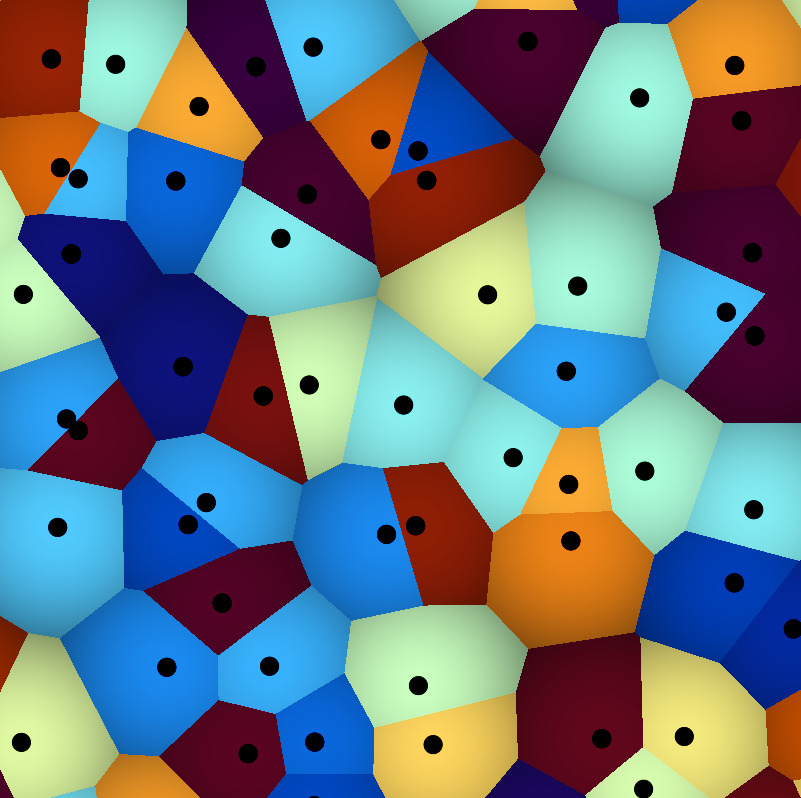
\includegraphics[width=0.32\textwidth]{figures/3-fastsim/voronoi.jpg}
  
\includegraphics[width=0.32\textwidth]{figures/3-fastsim/voronoi_apollonian.jpg}
  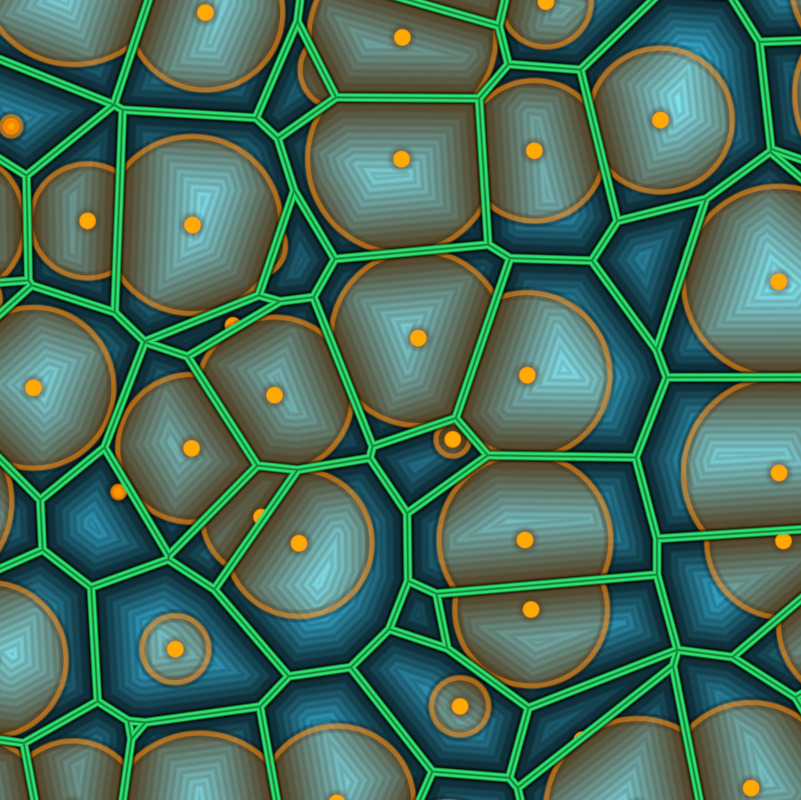
\includegraphics[width=0.32\textwidth]{figures/3-fastsim/voronoi_radical.jpg}
  \caption{Bidimensional illustrations of a Voronoi decomposition using three types of algorithm: (i) for equally sized circles using the equation~\ref{eq:voronoi_partition} (\url{www.shadertoy.com/view/MslGD8}) (ii) for unequally sized circles using the Apollonian Voronoi decomposition condition~\ref{eq:r_voronoi_apollonian} (\url{www.shadertoy.com/view/4sd3D7}) and (iii) another algorithm for unequally sized circles using the radical Voronoi condition~\ref{eq:r_voronoi_radical} (\url{www.shadertoy.com/view/4tV3z3}). Note that the second picture shows the curved boundaries between the Voronoi cells, while the switch to the radical Voronoi decomposition gives straight line boundaries.}\label{fgr:voronoi_illustration}
\end{figure}

This regular Voronoi tessellation is suitable only for separating space among equally sized atoms, as it sets the boundaries at equidistance from all the surrounding atoms, as shown in Figure~\ref{fgr:voronoi_illustration}. For atoms with unequal sizes, this type of definition may not be desirable, as the boundary could be closer to the surface of an atom compared to another. The initial rationale behind using a Voronoi decomposition is to delimit a region for each atom that is closer to that specific atom than any other. The ambiguity of this definition arises from the definition of ``closeness''. In this regular Voronoi decomposition, closeness is determined based on the distance between the center of mass of different atoms, which poses challenge for unequally distributed radii.

\subsubsection{Unequal radii}

To address this limitation, an alternative approach called the Apollonian Voronoi diagram can be implemented to model the atomic radii The definition of the Voronoi decomposition, as previously discussed, is limited to equal-sized atoms, as the closest region to an atom is also the closest to its center of mass. This limitation does not apply to the complex atomic structures found in nanoporous frameworks. To overcome this, the Apollonian Voronoi diagram\autocite{voronoi_apollonian} can be utilized to model the atomic radii $r_1,\ldots,r_n$ of points $\vect{x}_1,\ldots,\vect{x}_n$ within the same box $B$. For every $k\in\{1,\ldots,n\}$, the new subspaces $A_{k}$ are defined as follows:

\begin{equation}\label{eq:r_voronoi_apollonian}
  A_{k} = \left\{\vect{x} \in B\ \ |\ \ \forall\ l\neq k,\ {\lVert \vect{x}-\vect{x}_k \rVert}_2 - r_k \leq {\lVert \vect{x}-\vect{x}_l \rVert}_2 - r_l \right\}
\end{equation}

This new definition of the Voronoi diagram, takes into account the intuitive property of closeness to the atom's surface rather than its center of mass. This adjustment allows for an unequal distribution of atomic radii, as the diagram now depends on these radii. However, as illustrated in Figure~\ref{fgr:voronoi_illustration}, the initial implementation presents a convenient definition at the cost of curved edges, which introduces computational challenges.

To overcome these challenges and enhance computational efficiency, a less intuitive but more commonly used implementation known as the radical Voronoi tessellation, power diagram or Laguerre-Voronoi diagram\autocite{aurenhammer_1987} is preferred. As depicted in Figure~\ref{fgr:voronoi_illustration}, this method yields subspaces that are convex polygons with straight edges. Although the condition defining these subspaces is less intuitive, it avoids reliance on a simple definition. The subspaces $V_k$ are now defined based on the following condition:

\begin{equation}\label{eq:r_voronoi_radical}
    V_{k} = \left\{\vect{x} \in B\ \ |\ \ \forall\ l\neq k,\ {\lVert \vect{x}-\vect{x}_k \rVert}_2^2 - r_k^2 \leq {\lVert \vect{x}-\vect{x}_l \rVert}_2^2 - r_l^2 \right\}
  \end{equation}

In addition to the polyhedral form of the Voronoi cells, this new implementation presents interesting properties for porosity calculations in frameworks composed of unequal spheres, such as MOFs of zeolites.\autocite{voronoi_radical} First, the boundary between two overlapping spheres corresponds simply to the intersection between the spheres themselves. Secondly, the boundary between non-overlapping spheres always lies within the void space separating them. This assertion can easily be demonstrated by considering a point $\vect{x}$ in $V_{k}$ and ${\lVert \vect{x}-\vect{x}_k \rVert}_2 \geq r_k$ outside the sphere, which implies $\forall\ l\neq k$, ${\lVert \vect{x}-\vect{x}_k \rVert}_2 \geq r_k$. The point $\vect{x}$ does not overlap with any other atom and resides within the framework's void space.

When considering a point $\vect{v}$ on a boundary between $p$ Voronoi cells, denoted as $\left\{V_{i_1},\ldots,V_{i_p}\right\}$, this point satisfies the conditions ${\lVert \vect{x}-\vect{x}_{i_1} \rVert}_2^2 - r_{i_1}^2 = \cdots = {\lVert \vect{x}-\vect{x}_{i_p} \rVert}_2^2 - r_{i_p}^2 = C$. It is possible to find the minimum distance to the center of mass of neighboring atoms and test possible overlapping. Specifically, in the Zeo++ software,\autocite{Zeo++} the Voronoi diagram is characterized by storing the minimum distance to the closest atoms and the corresponding atom indices for each vertex and edge (In cases where edges connect two different periodic images, a periodic displacement vector is also stored). Leveraging this information enables the acceleration of void fraction calculations by bypassing volume calculations in non-adsorbable Voronoi cells. Additionally, it provides a swift approach to determine accessible and non-accessible surface areas and volumes.\autocite{Zeo++} It is important to note that when employing a probe with a radius $r\e{probe}$, the sphere radii considered are adjusted accordingly as $r_k = r\e{atom}+r\e{probe}$.

\subsection{Implementation in a screening}


The use Voronoi decomposition for geometric characterization of the pore space in materials has become widespread in computational studies over the past decade.\autocite{Willems_2012} Its popularity increased notably after its incorporation into the Zeo++ software package.\autocite{Pinheiro2013} Recently, this technique was further extended to implement a novel sampling scheme in a study focused on ML-assisted screening of nanoporous materials for xenon/krypton separation. In their work, Simon et al.\autocite{Simon_2015} relied on a Voronoi tessellation of the nanoporous materials and assigned the potential adsorption sites (i.e., the sampling points) at the nodes of this decomposition. The Voronoi tessellation identifies the vertices of polyhedra that correspond to the closest regions to each atom in the structure. These vertices (or \emph{Voronoi nodes}) are the points equidistant to at least four atoms of the structure, and can be associated with adsorption sites due to their closeness to the center of the pores. 

The Zeo++ software definition of accessibility was used in a screening process aimed at identifying optimal materials for Xe/Kr separation.\autocite{Simon_2015} The interaction energies of xenon were calculated exclusively at the accessible nodes, as illustrated in Figure~\ref{fgr:simon_voro}. The average of the energies at these accessible Voronoi nodes provided an estimation of the adsorption enthalpy. However, this sampling approach assumes that the nodes are close to the actual and most favorable adsorption sites, which implies that the the adsorption sites are located at the center of the pores. This assumption holds true only for structures with pore sizes similar to that of the adsorbate. The newly defined adsorption energy descriptor was identified as one of the most influential descriptors in the ML learning model developed to predict ambient-pressure selectivity.

\begin{figure}[ht]
  \centering
  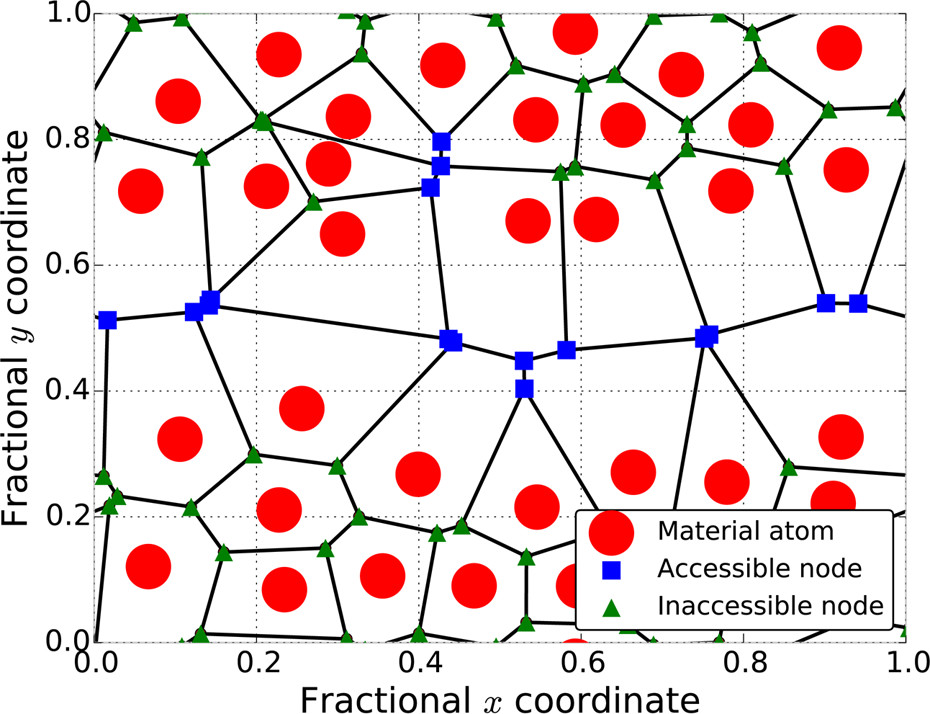
\includegraphics[width=0.5\textwidth]{figures/3-fastsim/Simon_voronoi.jpeg}
  \caption{Voronoi network model of void space (2D caricature). The unit cell of a toy material is shown. Red circles represent atoms of the material; accessible and inaccessible Voronoi nodes are blue squares and green triangles, respectively. The black lines are the edges in the periodic Voronoi graph that model the void space. Reprinted with permission from Ref.~\cite{Simon_2015}. Copyright 2015 American Chemical Society.}\label{fgr:simon_voro}
\end{figure}

In light of the initial Voronoi sampling methodology, it is worth questioning the relevance of directly averaging the interaction energies instead of employing Boltzmann averaging to describe the adsorption enthalpy. To gain a deeper understanding of the strengths and weaknesses of this methodology, different methods for approximating adsorption enthalpies have been compared through the Voronoi sampling approach with more accurate infinite dilution and ambient-pressure xenon adsorption enthalpies using Widom insertions and GCMC for a 20:80 Xe/Kr mixture at \SI{1}{\atm} and \SI{298}{\kelvin}.

\subsection{Comparative study of the Voronoi sampling}

In the previous chapter, the definition of the xenon adsorption enthalpy at infinite dilution (Widom insertion section~\ref{sct:widom}) and at ambient pressure (GCMC sections~\ref{sct:GCMC} and~\ref{sct:thermo}) was introduced. These methods are widely acknowledged for their accuracy in calculating adsorption enthalpies, which have been established as strongly correlated with the logarithm of selectivity in a previous study on the thermodynamic exploration of xenon/krypton separation using high-throughput screening.

\subsubsection{Introduction of the main concepts}

The Voronoi energy, as initially conceptualized by Simon et al.,\ is obtained by averaging the xenon interaction energies at the accessible Voronoi nodes. However, for the purpose of comparing with thermodynamic simulations without blocking pockets, the focus is shifted from the accessible Voronoi nodes to the adsorbable Voronoi nodes as they provide a closer approximation to the desired simulation. To simplify the analysis, the set of the adsorbable Voronoi nodes $A$ is defined as the Voronoi nodes with a negative energy value. Additionally, a minimum distance condition is applied (approximately equal to the radius of a xenon \SI{2}{\angstrom}) to reduce the number of points that need to be calculated. This average on the adsorbable Voronoi nodes $E\e{voro-A}^{Xe}$ can be expressed as follows:

\begin{equation}
    E\e{voro-A}^{Xe} = \sum_{i \in A} E_i -RT
\end{equation}

Another interesting energy descriptor could simply be the minimum of the interaction energies among the Voronoi nodes $V$ with a minimum distance to the nearest atom higher than \SI{2}{\angstrom}. This minimum Voronoi energy $E\e{voro-M}^{Xe}$ can be expressed as follows: 

\begin{equation}
    E\e{voro-M}^{Xe} = \min_{i \in V} E_i
\end{equation}

Finally, to align with the definition of the heat of adsorption presented in the previous chapter, an energy descriptor can be built using a Boltzmann averaging. This Boltzmann average of the xenon interaction energies at the Voronoi nodes $V$ is denoted as $E\e{voro-B}^{Xe}$ and can be expressed as follows:

\begin{equation}
    E\e{voro-B}^{Xe} = \dfrac{\sum\limits_{i \in V} E_i e^{-\beta E_i}}{\sum\limits_{i \in V} e^{-\beta E_i}} -RT
\end{equation}
It should be noted that the $-RT$ term is necessary to make the expression comparable to the one of adsorption enthalpy. 

Intuitively, since Boltzmann averaging is closer to the definition of the adsorption enthalpy, it would be a more suitable candidate as an energy descriptor, potentially improving the screening methodology. To test these different methodologies, various energy descriptors will be compared with a more accurate evaluation of the adsorption heat. 

\subsubsection{Low-pressure comparison}

The Widom insertion is typically used to calculate the infinite dilution adsorption properties, such as adsorption enthalpy, Henry constant and selectivity. The evaluation of xenon interaction energies at different Voronoi nodes corresponds to a low-pressure averaging and is more comparable to the Widom insertion method. However, it is biased by the inhomogeneous sampling of the space, which can account for some of the observed discrepancies.

It is important to note that in this chapter, the standard pore size definition commonly used in the literature, based on atom radii provided by the Cambridge Crystallographic Data Centre (CCDC), will be predominantly used. This pore size will only serve a labeling purpose aid in classifying structures based on their relative size. It predominantly plays a qualitative role, which justifies the omission of a more precise definition based on the forcefield, as employed in the previous chapter.

As illustrated in Figure~\ref{fgr:compa_voro_0}, the average of energies exhibits suboptimal performance and demonstrates weaker correlation with the adsorption enthalpy compared to the minimum interaction energy or the Boltzmann average of interaction energies. This discrepancy occurs because, in a normal average, high-energy values carry a disproportionately higher weight than in a Boltzmann average, resulting in the average being more significant than expected. The Voronoi average descriptor $E\e{voro-A}^{Xe}$ consistently yields higher values than the infinite dilution adsorption enthalpy $\Delta\e{ads} H_{0}\ex{Xe}$. 

\begin{figure}[ht]
  \centering
    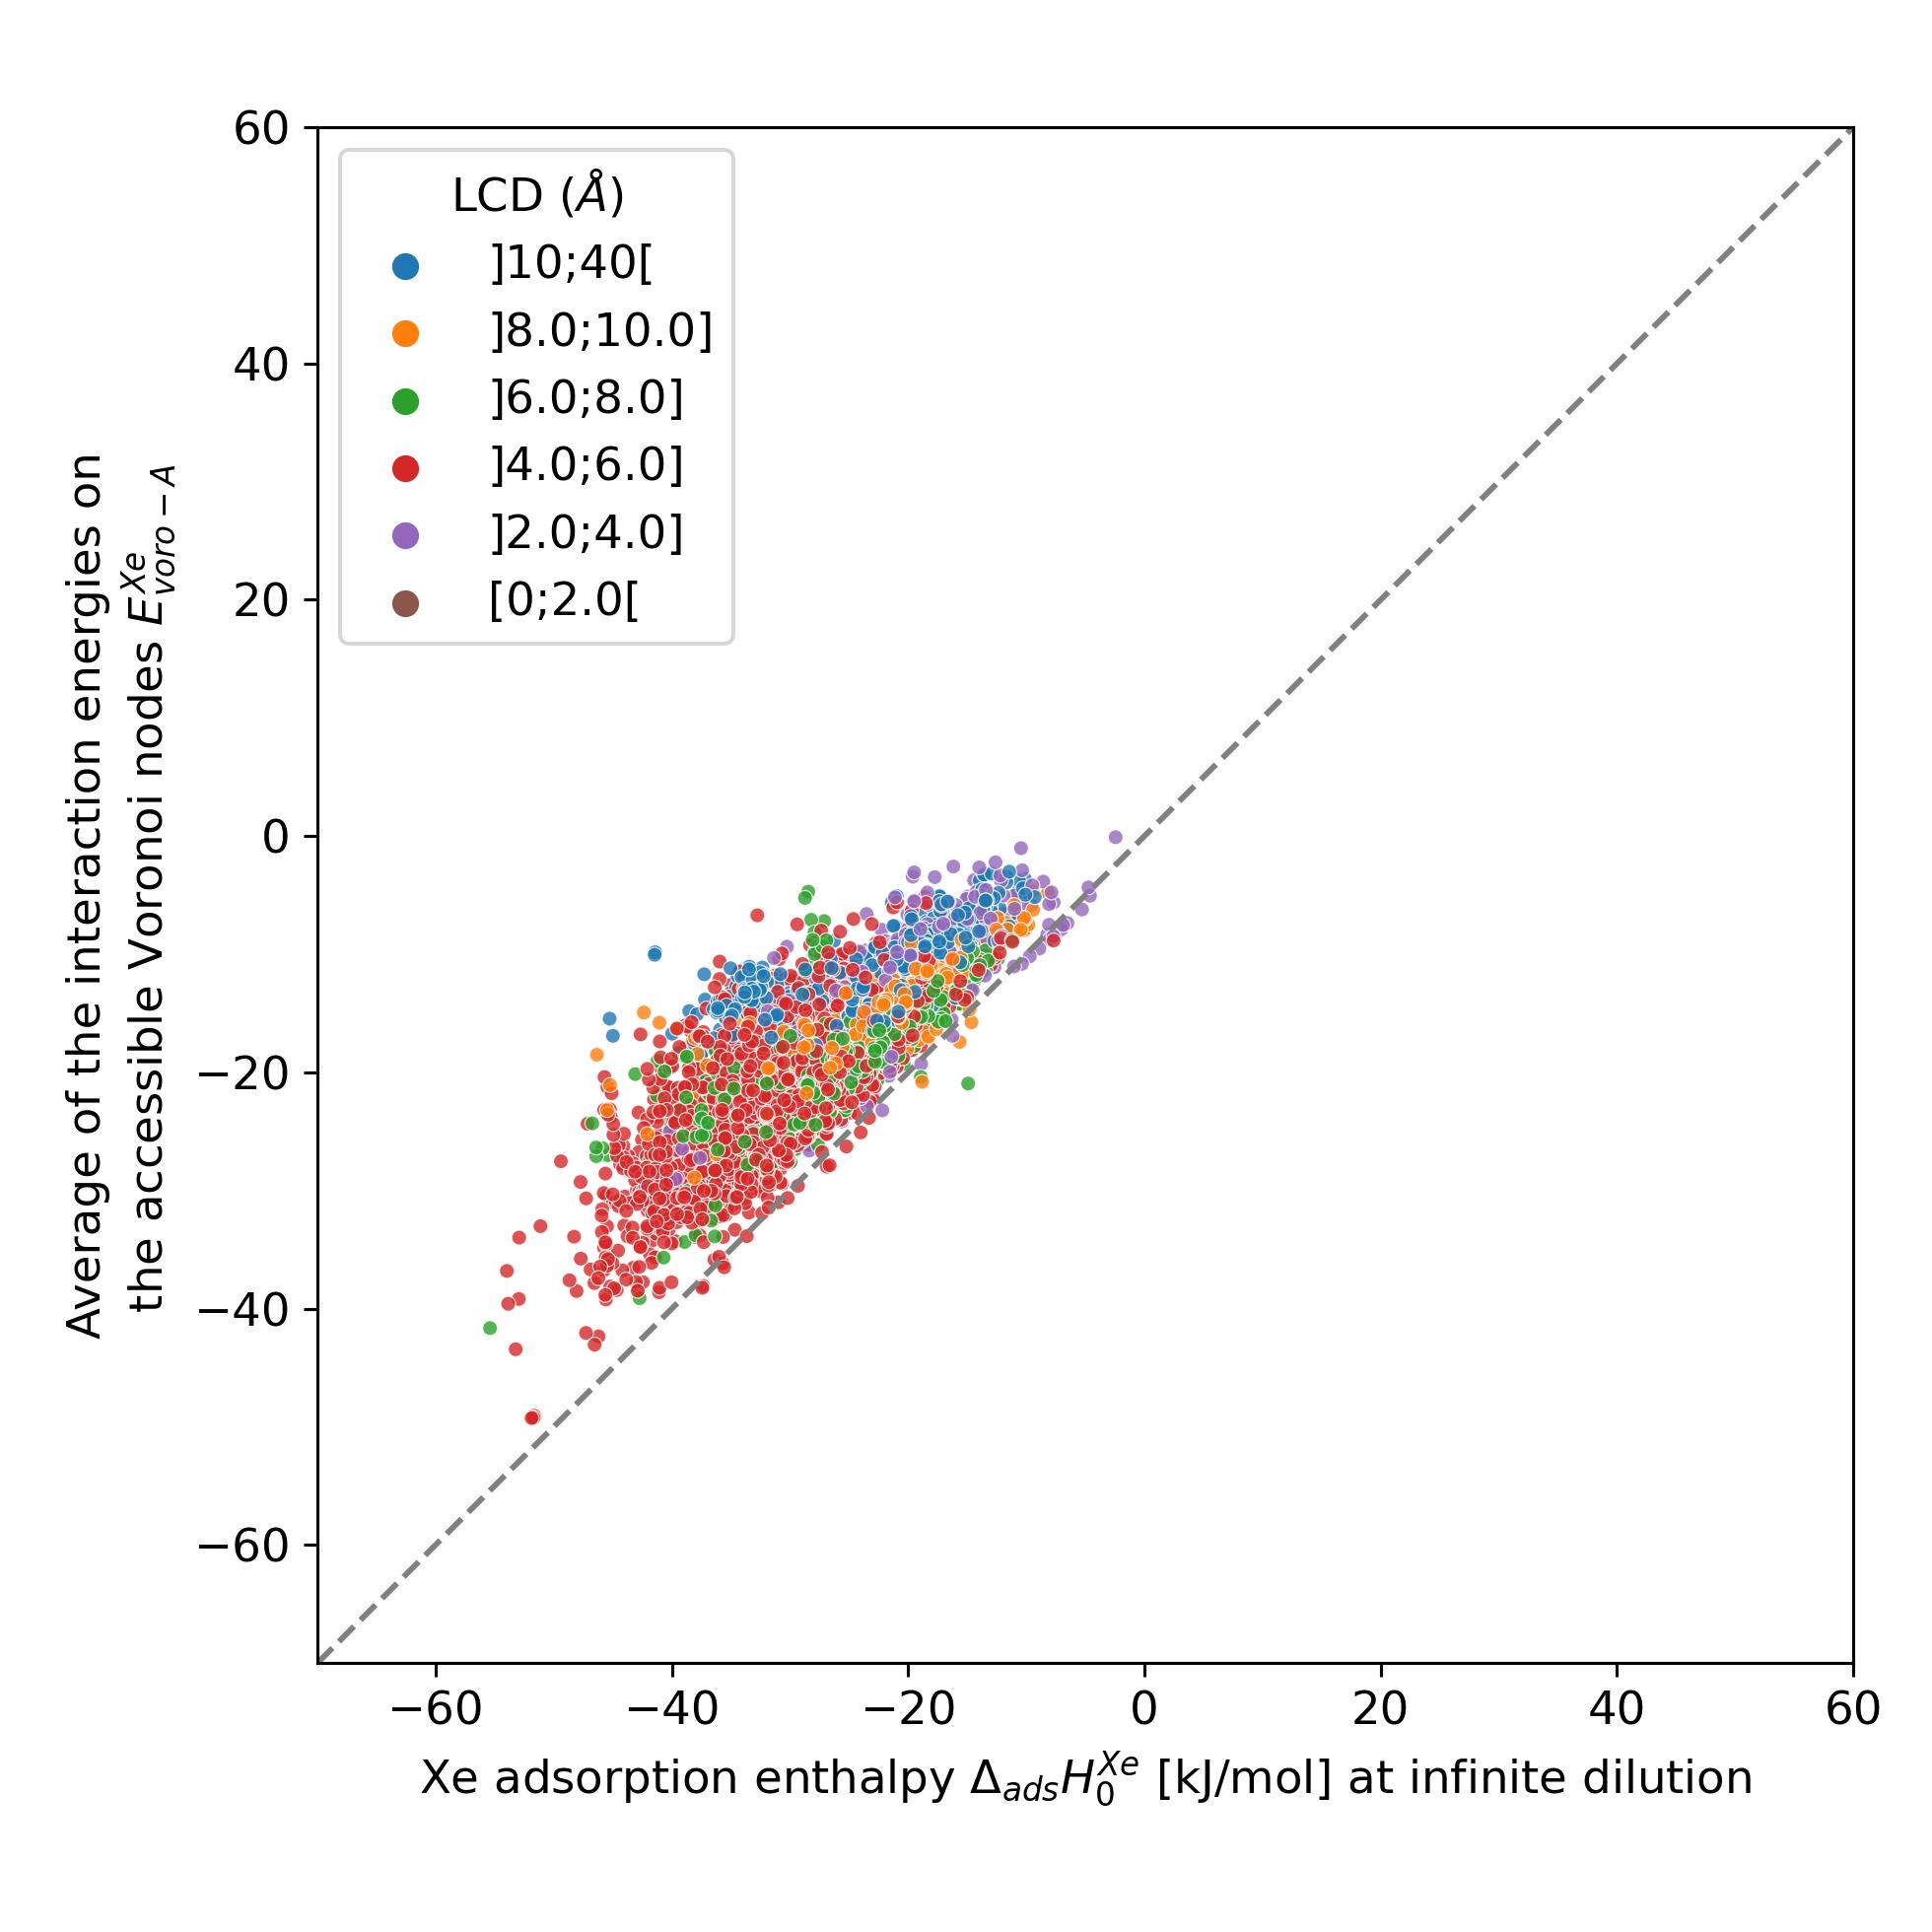
\includegraphics[width=0.32\textwidth]{figures/3-fastsim/H_Xe_0_vs_E_voro_A_overview.jpg}
    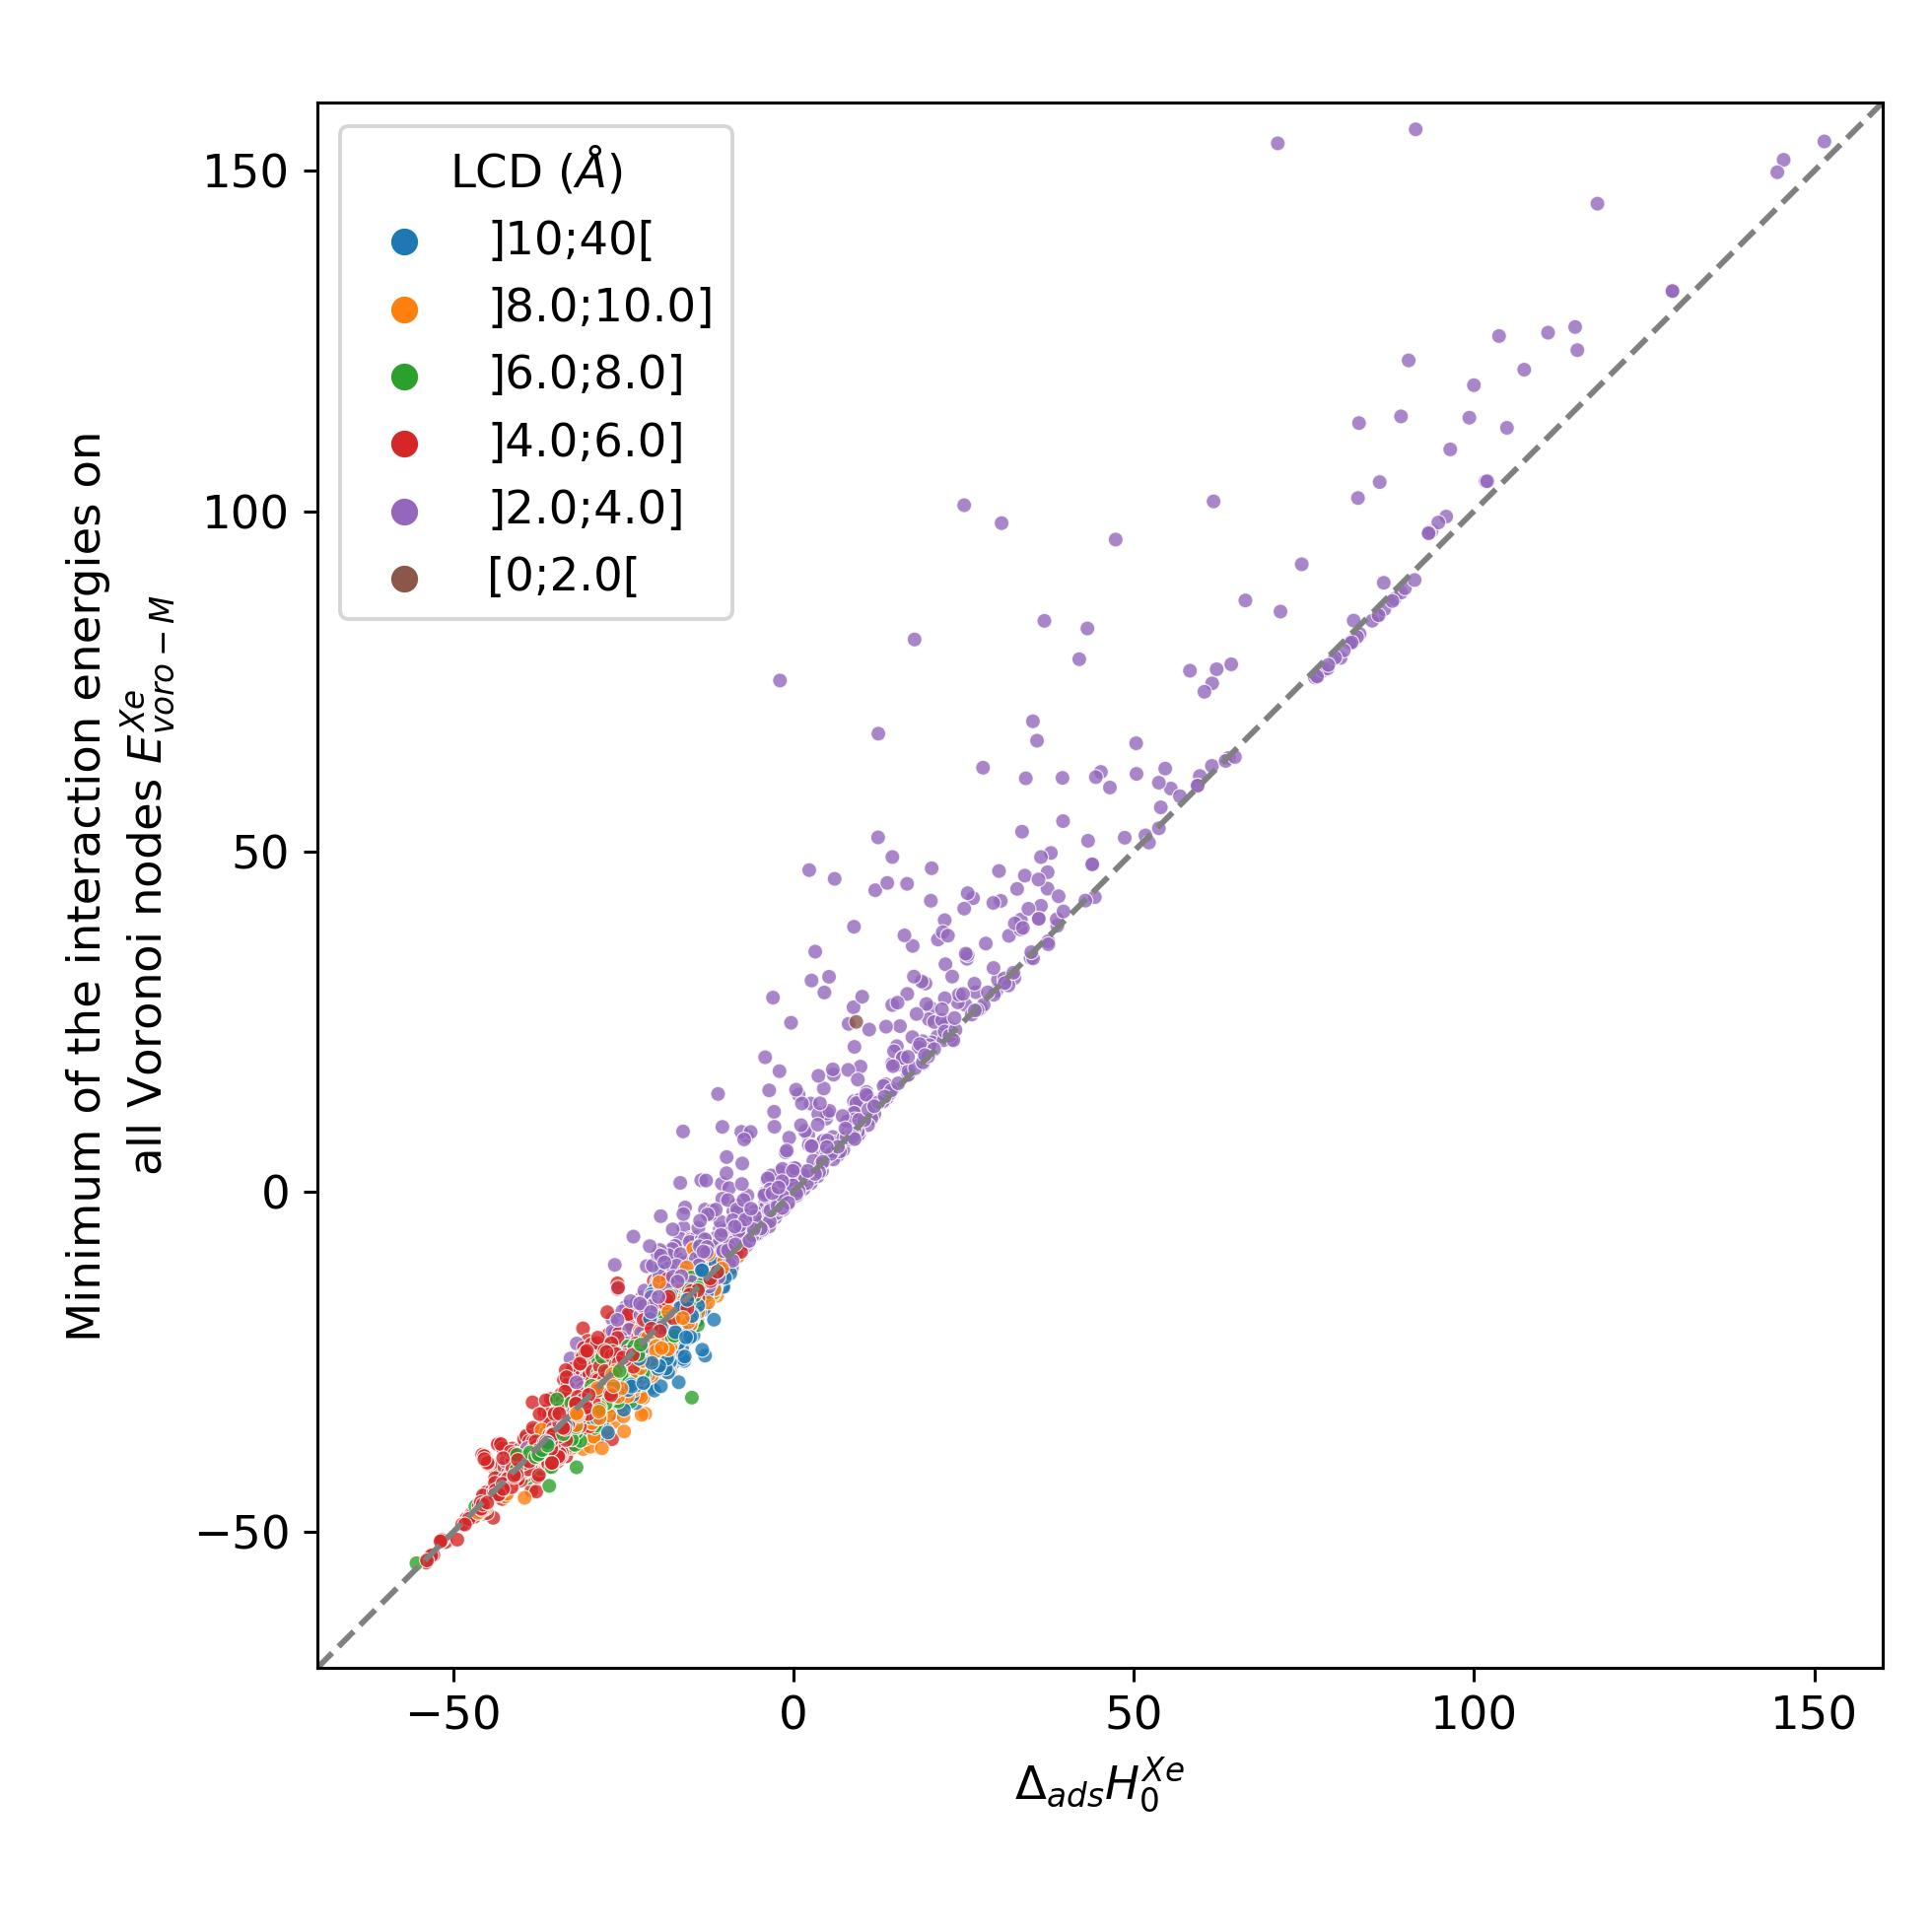
\includegraphics[width=0.32\textwidth]{figures/3-fastsim/H_Xe_0_vs_E_voro_M_overview.jpg}
    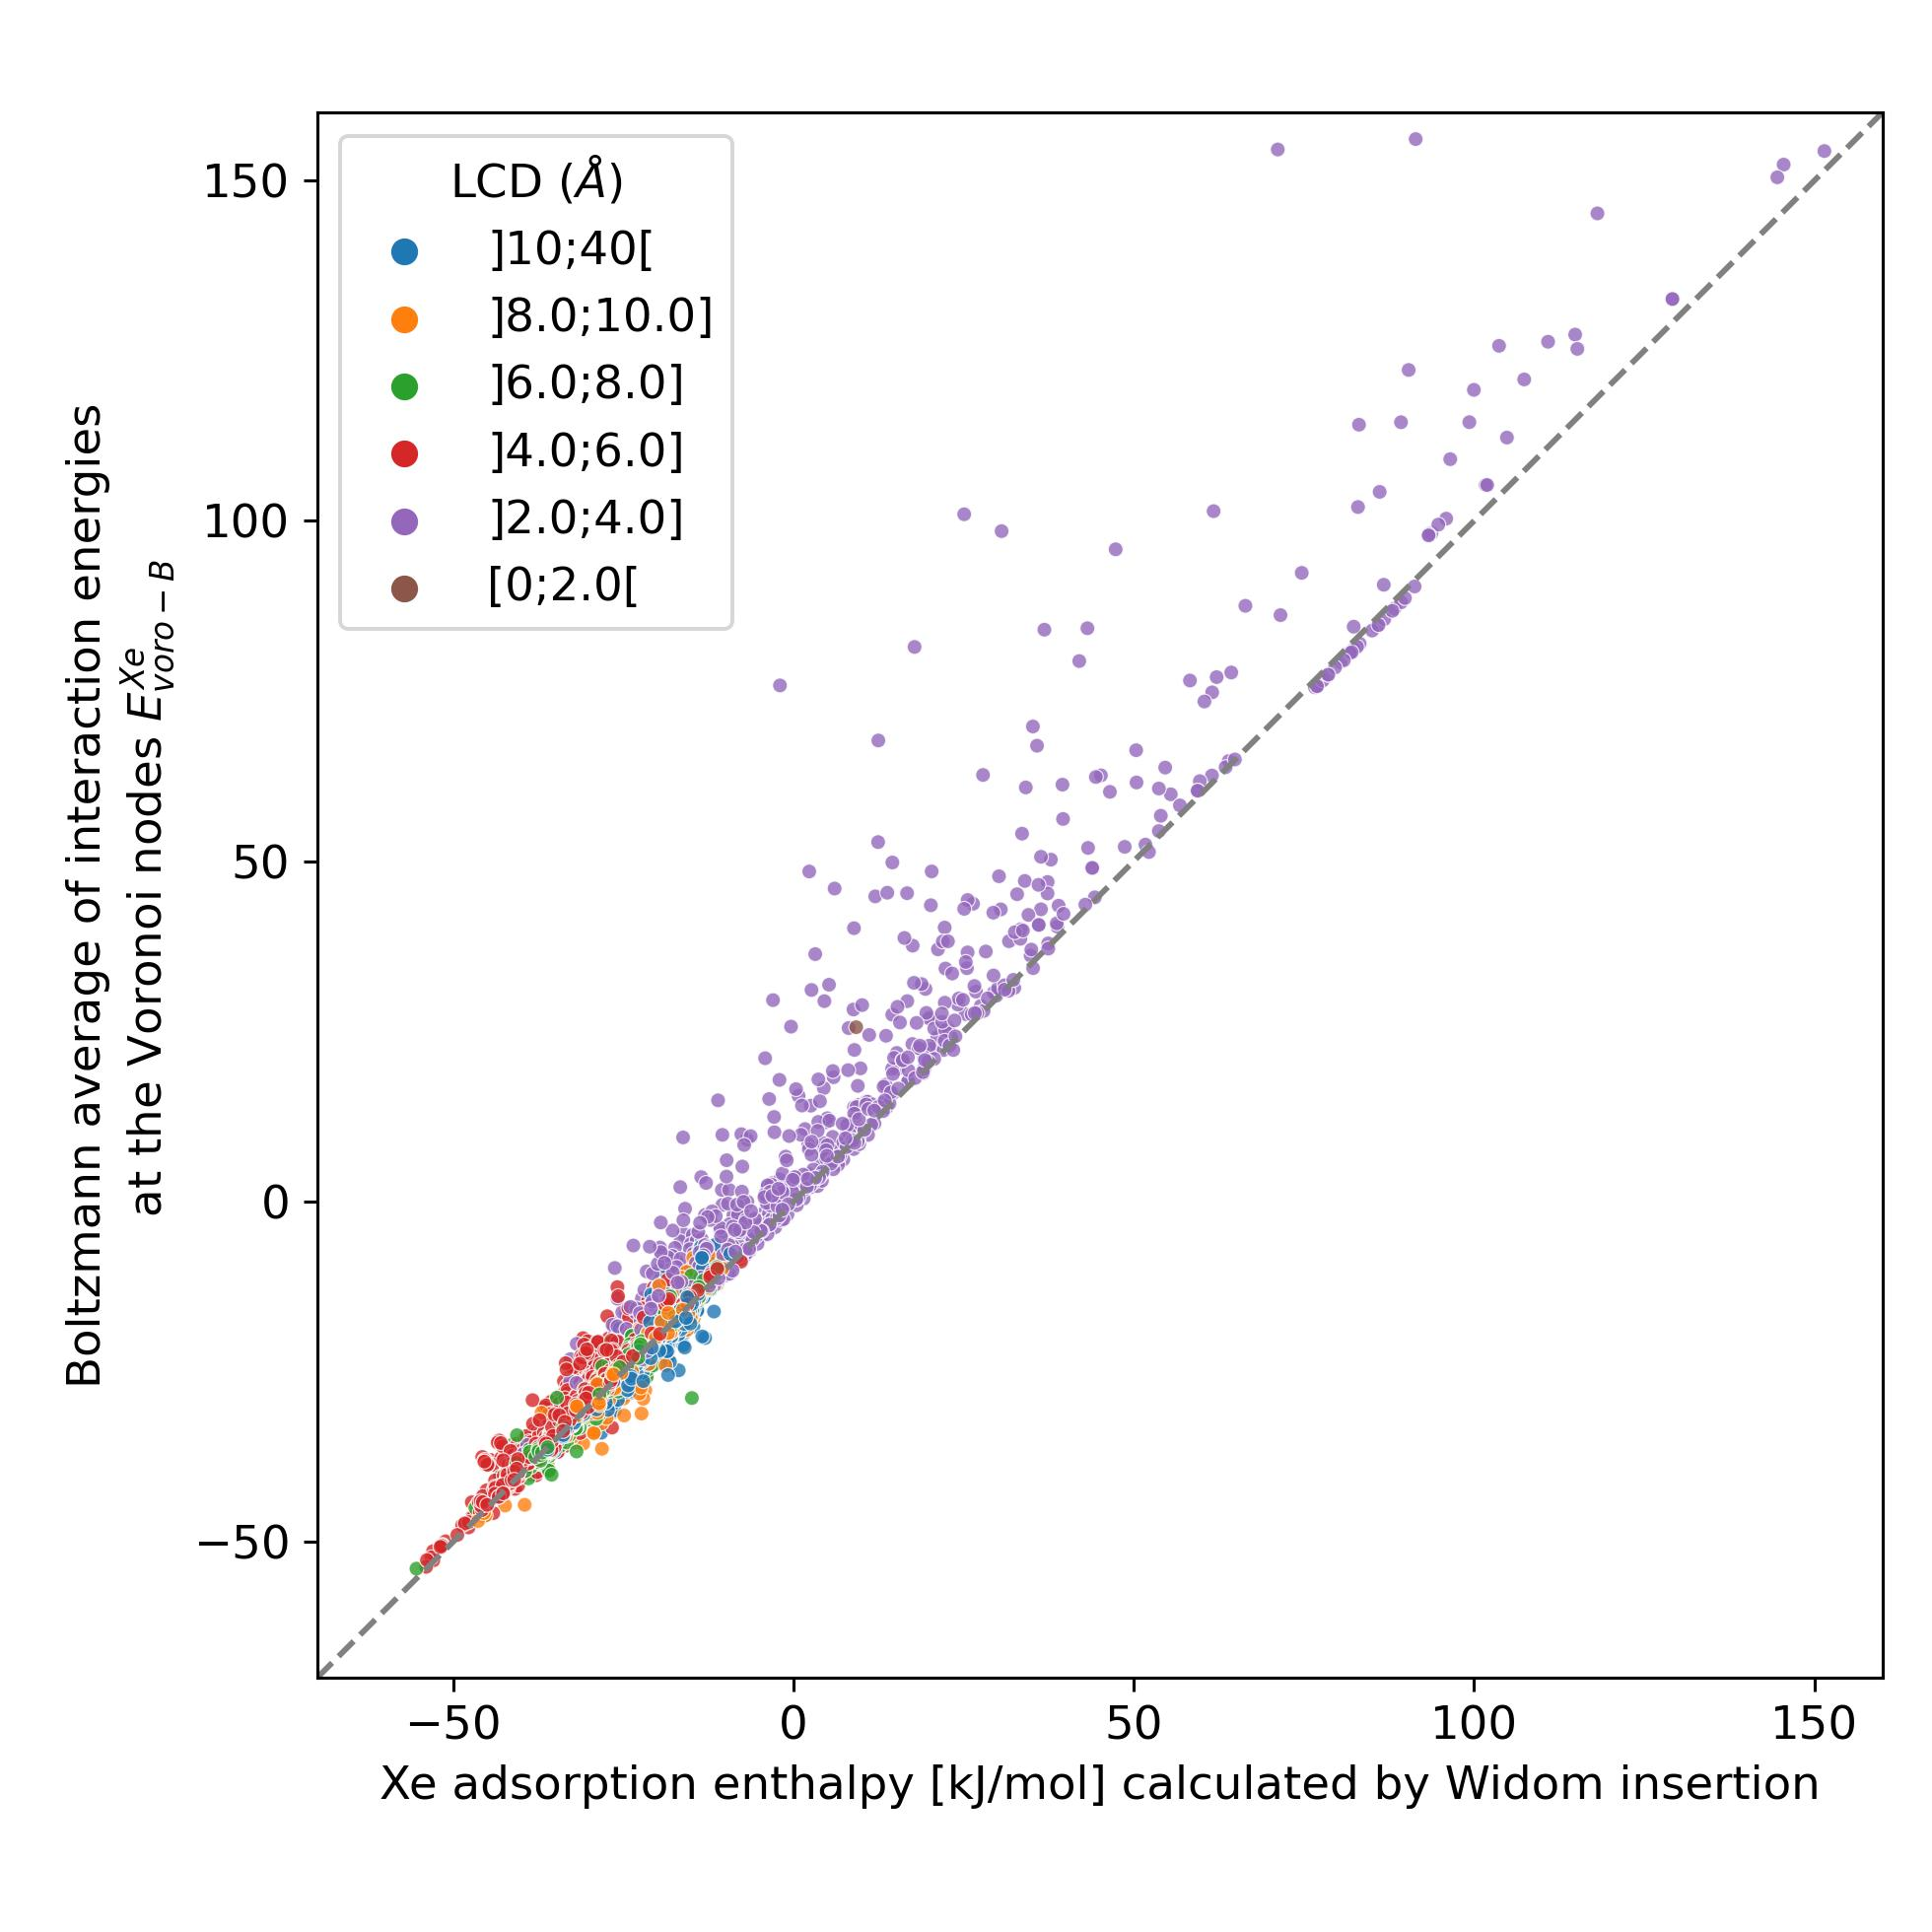
\includegraphics[width=0.32\textwidth]{figures/3-fastsim/H_Xe_0_vs_E_voro_B_overview.jpg}
    \caption{Scatterplots of the energy descriptors $E\e{voro-A}^{Xe}$, $E\e{voro-M}^{Xe}$ and $E\e{voro-B}^{Xe}$ calculated by a Voronoi sampling compared to the enthalpies calculated by a 100k-step Widom insertion simulation of xenon in structures of CoRE MOF 2019. The points are labeled according to the largest cavity diameter (LCD\e{CCDC}) belonging to one of the intervals.}\label{fgr:compa_voro_0}
\end{figure}

The Pearson correlation coefficients corroborate the initial observation made in this thesis. The correlation coefficient between $E\e{voro-A}^{Xe}$ and $\Delta\e{ads} H_{0}\ex{Xe}$ is $0.81$, whereas for the minimum $E\e{voro-M}^{Xe}$ and for the Boltzmann average $E\e{voro-B}^{Xe}$, it is respectively equal to $0.95$ and $0.97$. Based on these coefficients, it is evident that the Boltzmann average is more suitable to evaluate the relevance of a Voronoi energy sampling. As shown in the previous chapter, selectivity is correlated with the difference of adsorption enthalpies between xenon and krypton. Improving the description of enthalpy is a first key step towards a better description of selectivity. As the previous analysis only focused on selectivity values at low pressure, it is essential to explore the behavior of selectivity at higher pressures.

\begin{figure}[ht]
  \centering
  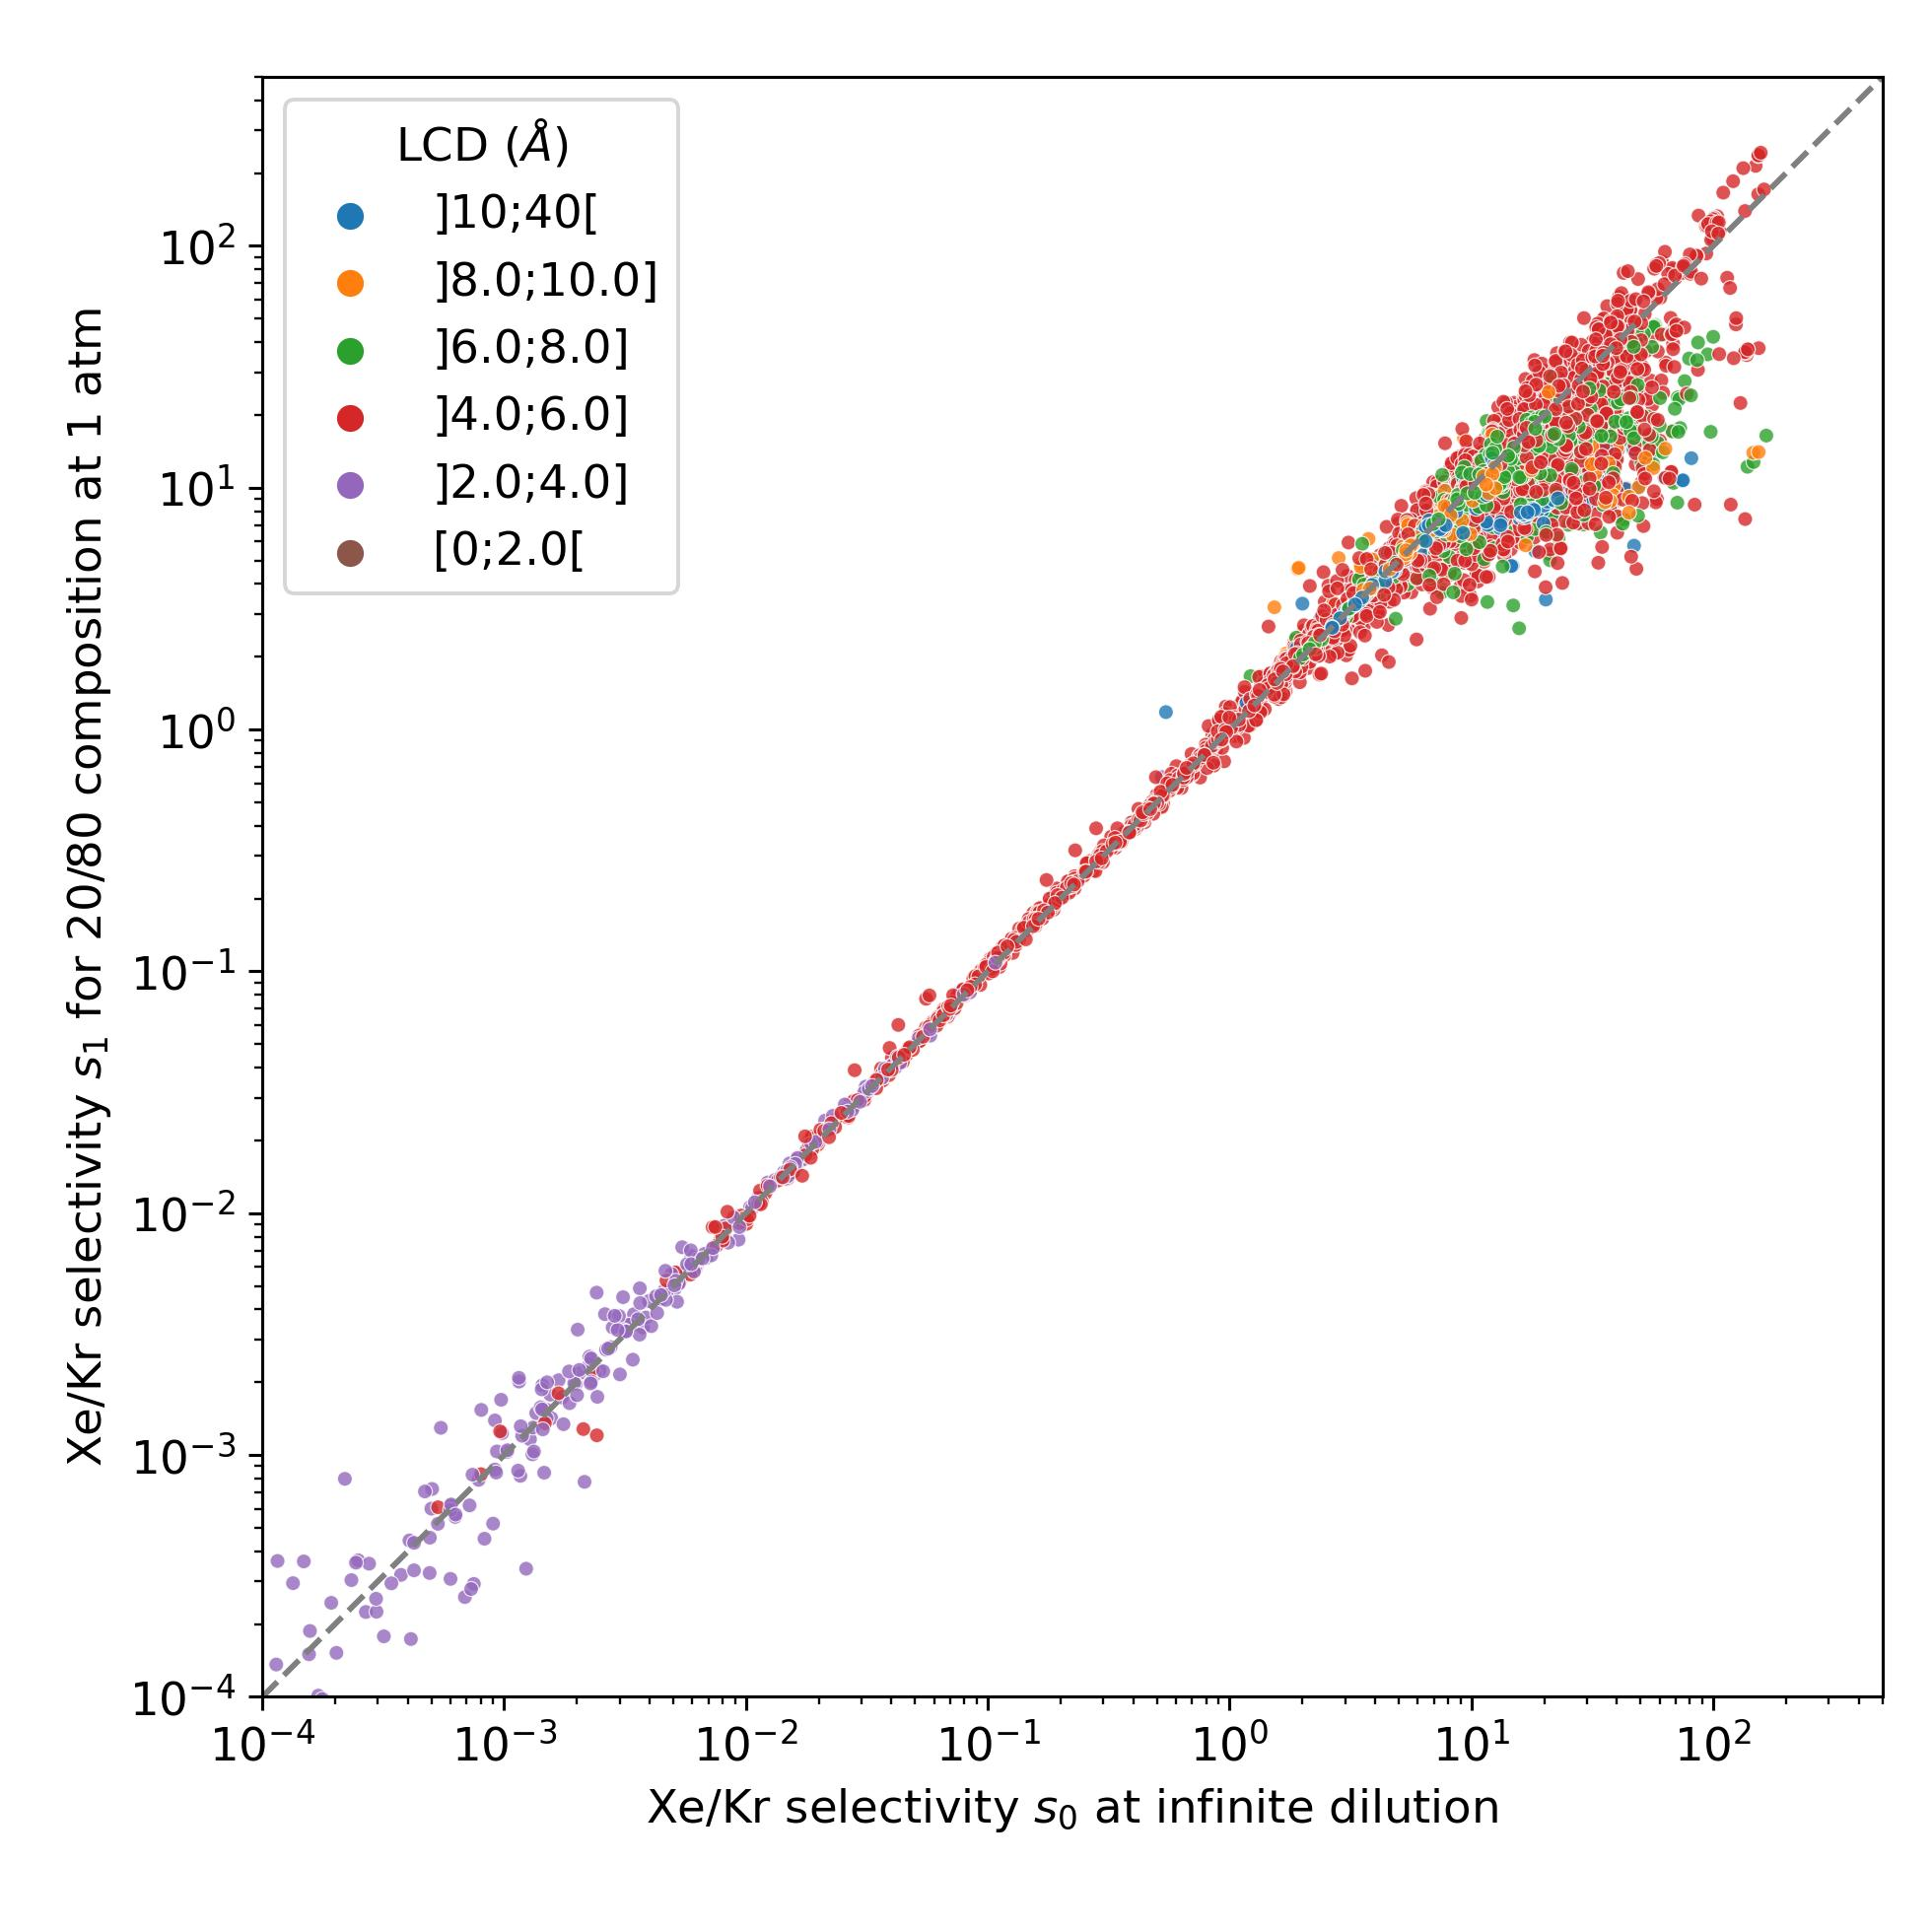
\includegraphics[width=0.45\textwidth]{figures/3-fastsim/s_0_vs_s_2080_overview.jpg}
  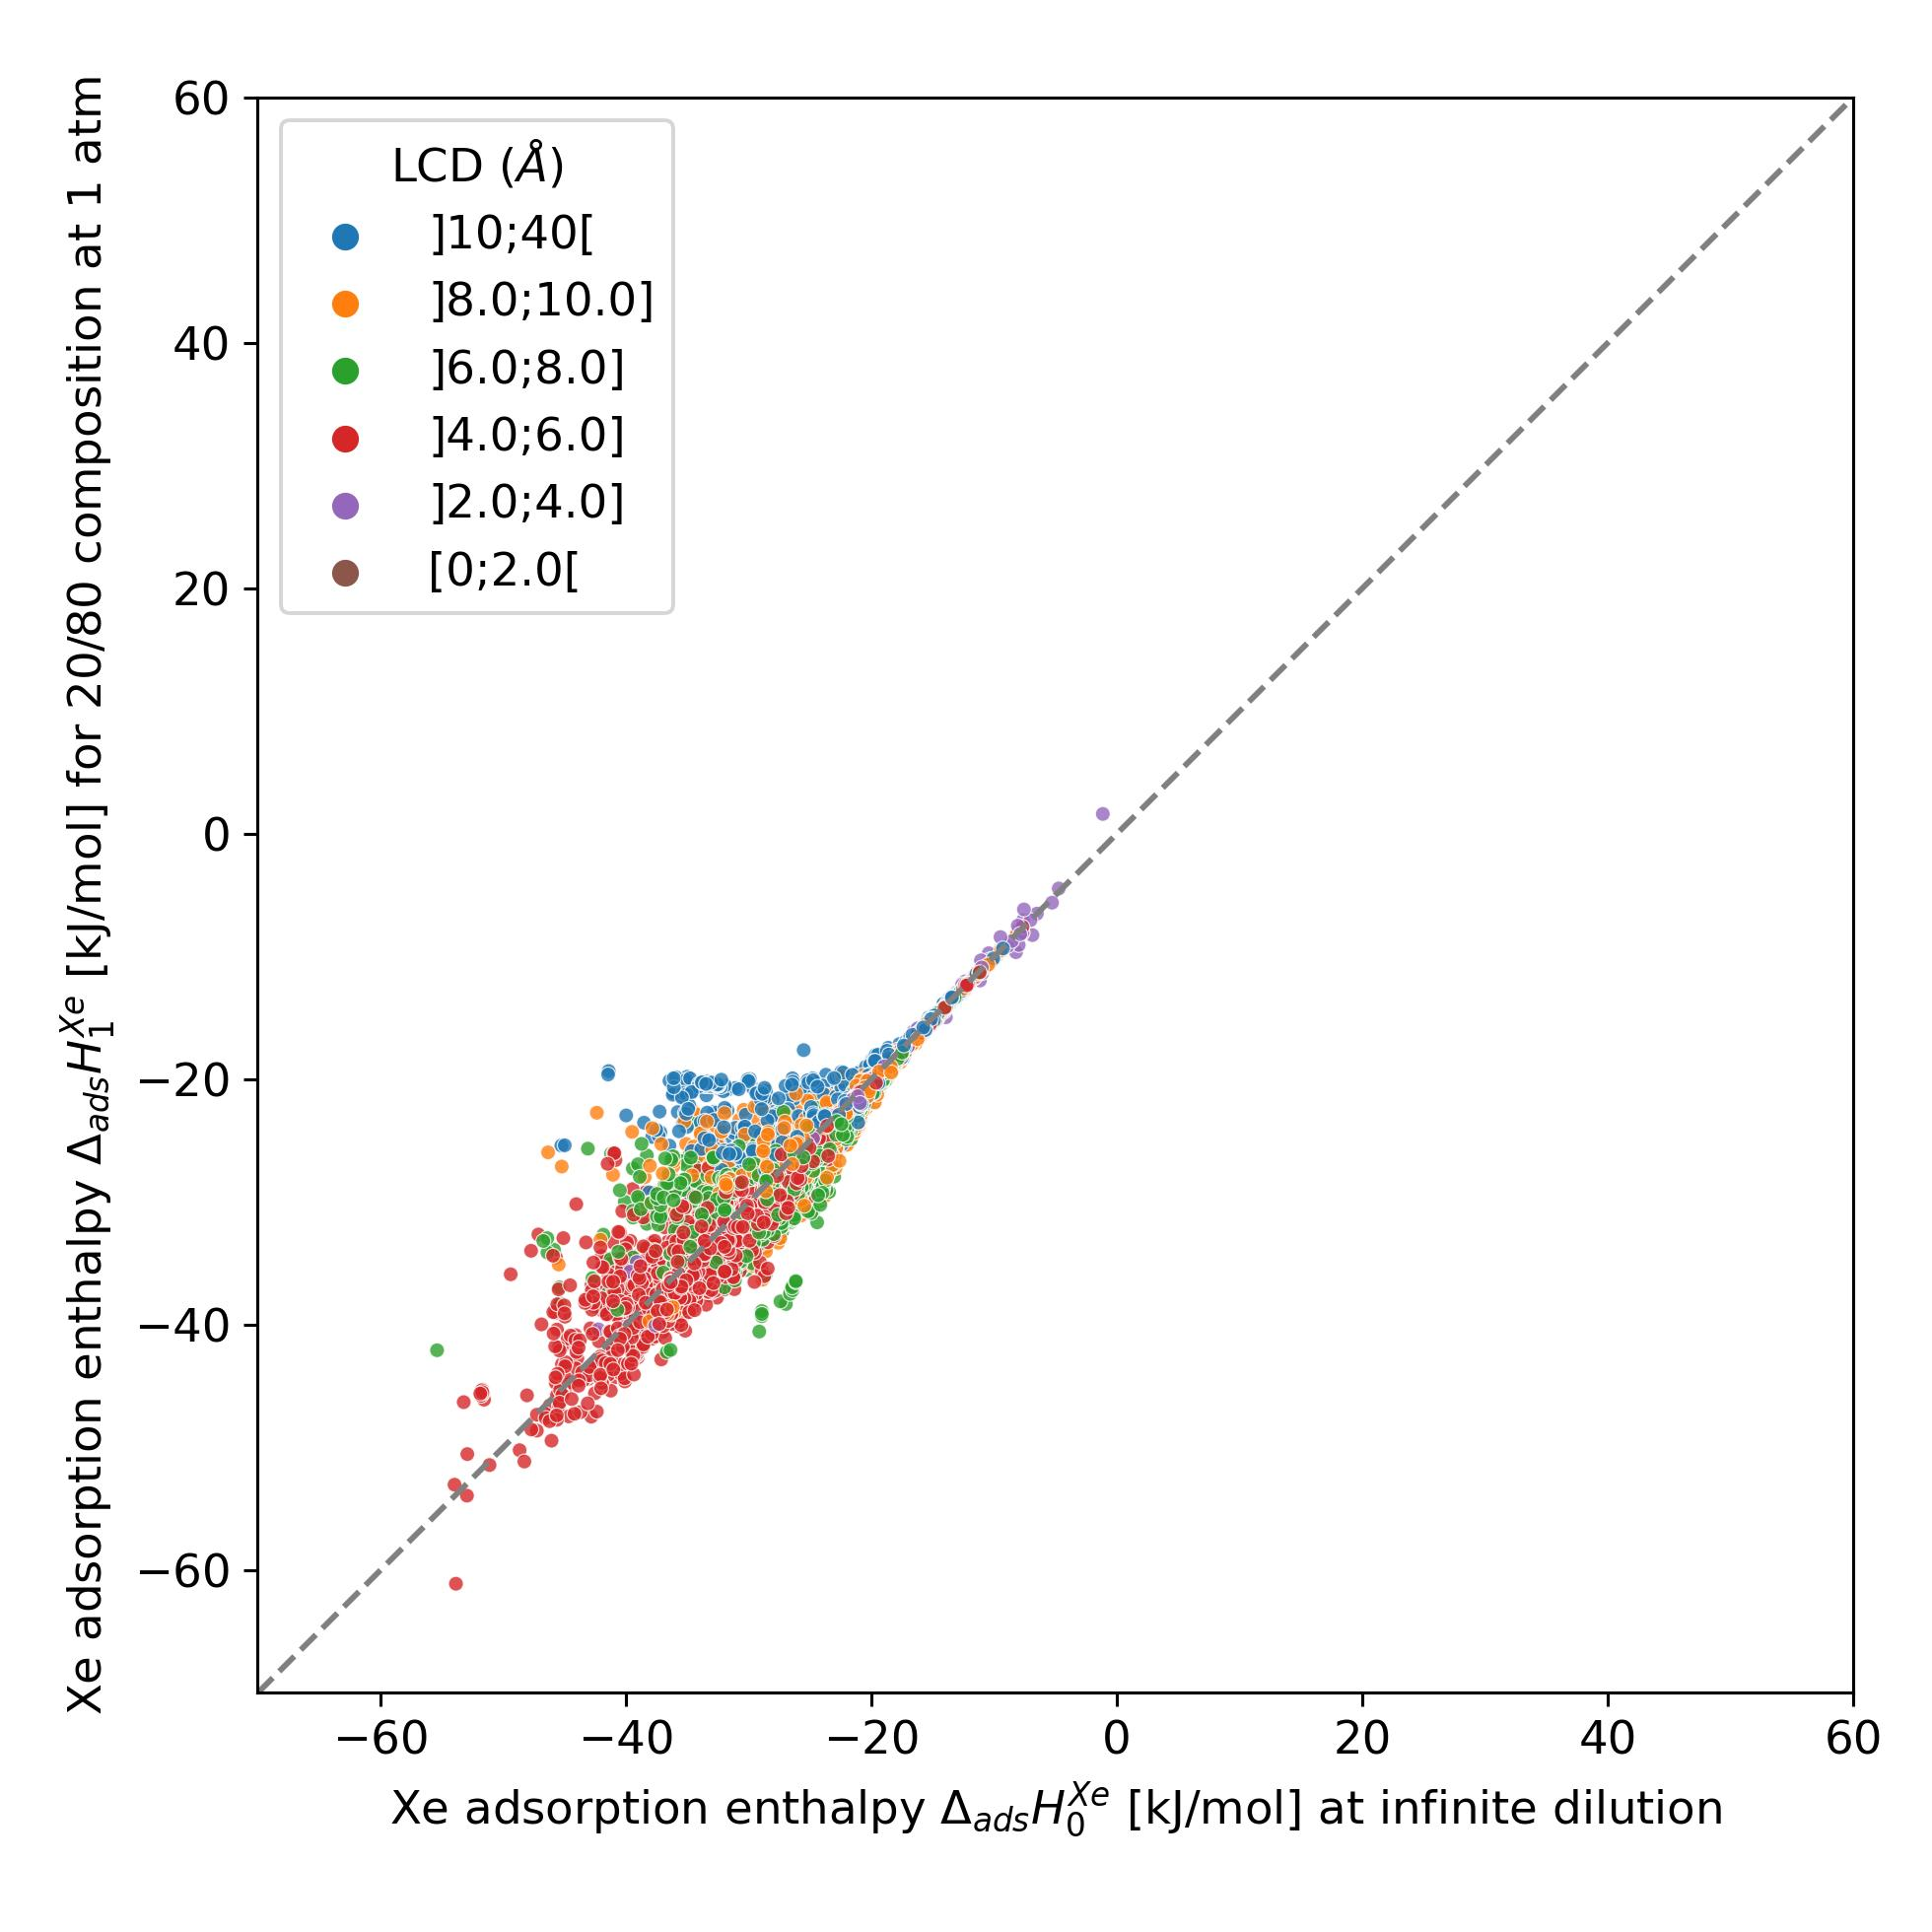
\includegraphics[width=0.45\textwidth]{figures/3-fastsim/H_Xe_0_vs_H_Xe_2080_overview.jpg}
    \caption{Comparison of the ambient-pressure and low-pressure case through two thermodynamic quantities: the Xe/Kr selectivity (left) and the xenon adsorption enthalpy (right). }\label{fgr:compa_pressure}
\end{figure}

Figure~\ref{fgr:compa_pressure} illustrates that the selectivity drop between the low-pressure and ambient-pressure cases has an impact on the enthalpy values of xenon. The xenon affinity decreases as the pressure increases. While the study conducted by Simon et al.\ primarily focused on predicting ambient-pressure selectivity, it is worth investigating whether the energy descriptor they developed can also describe the adsorption enthalpy at high pressure.

\subsubsection{Ambient-pressure xenon/krypton separation}

Upon observing the Figure~\ref{fgr:compa_voro_2080}, it is not clear which descriptor performs better in describing the enthalpy at ambient pressure. The scatterplots indicate similarly modest correlations for all descriptors, suggesting that the use a regular average may suffice instead of a Boltzmann average. The correlation coefficient for the average $E\e{voro-A}^{Xe}$ is now $0.86$, which is equivalent to both the minimum descriptor $E\e{voro-M}^{Xe}$ and slightly lower than the $0.87$ for the Boltzmann average $E\e{voro-B}^{Xe}$. 

\begin{figure}[ht]
    \centering
      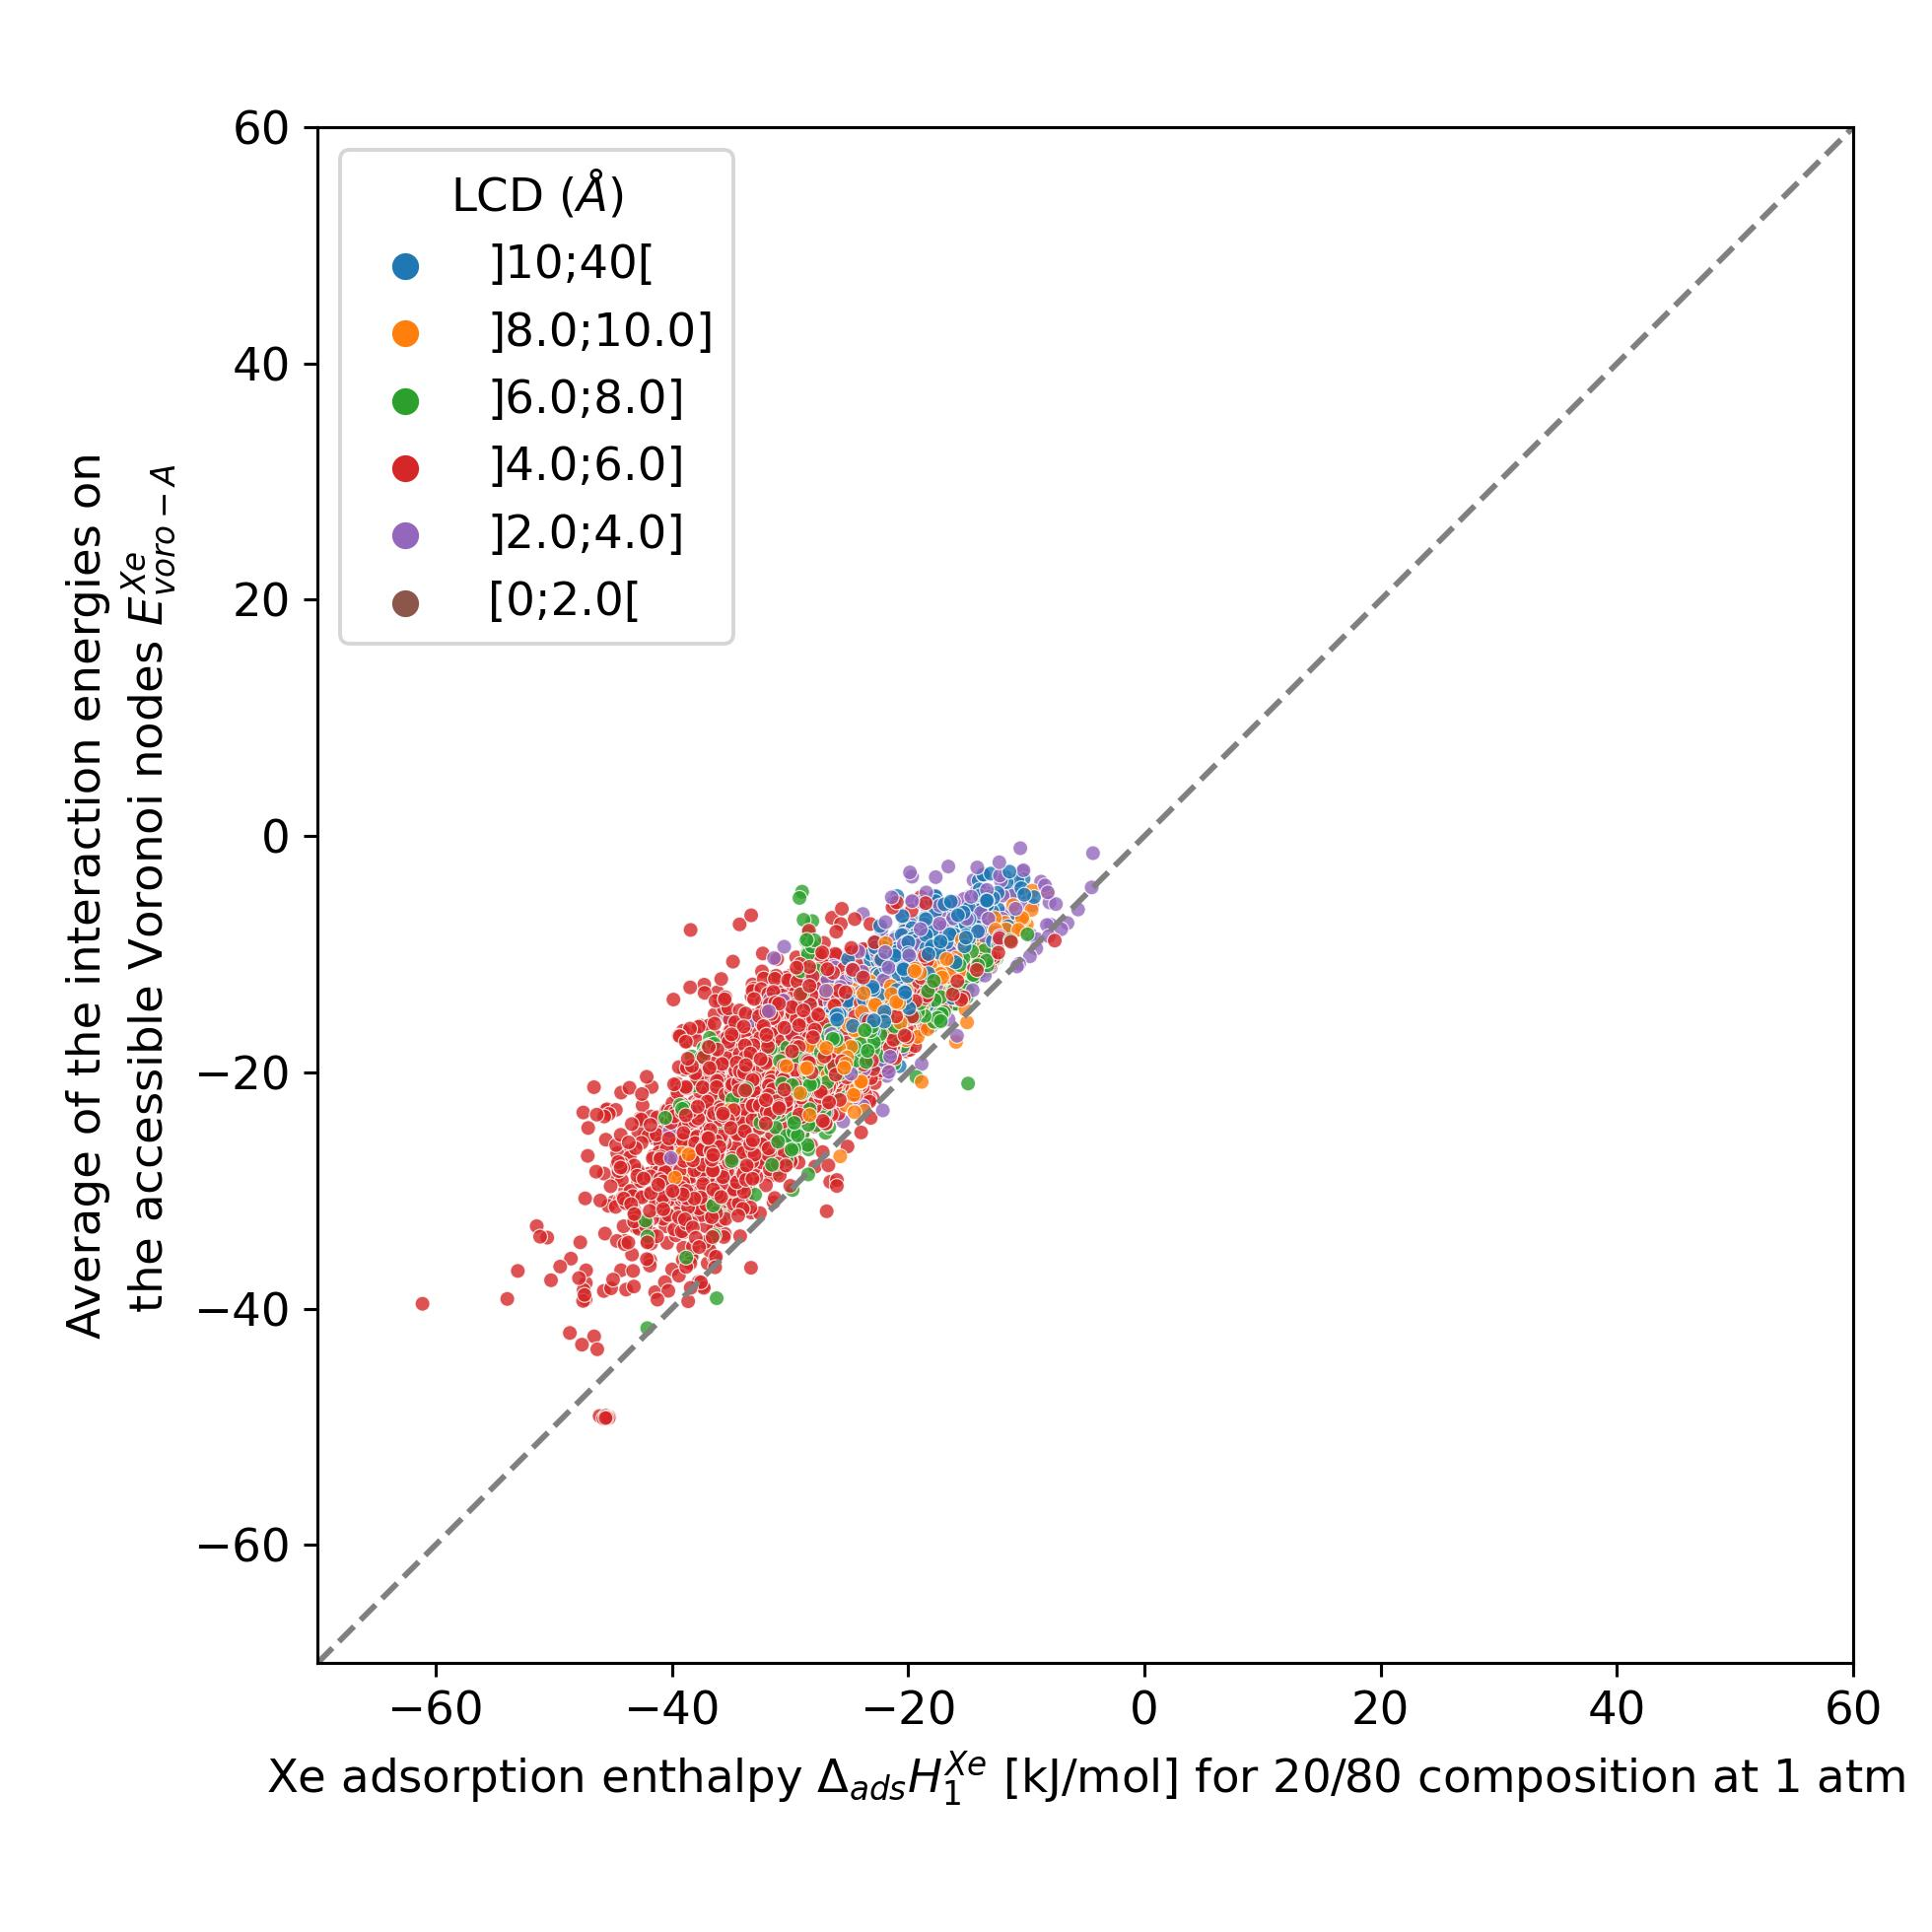
\includegraphics[width=0.32\textwidth]{figures/3-fastsim/H_Xe_2080_vs_E_voro_A_overview.jpg}
      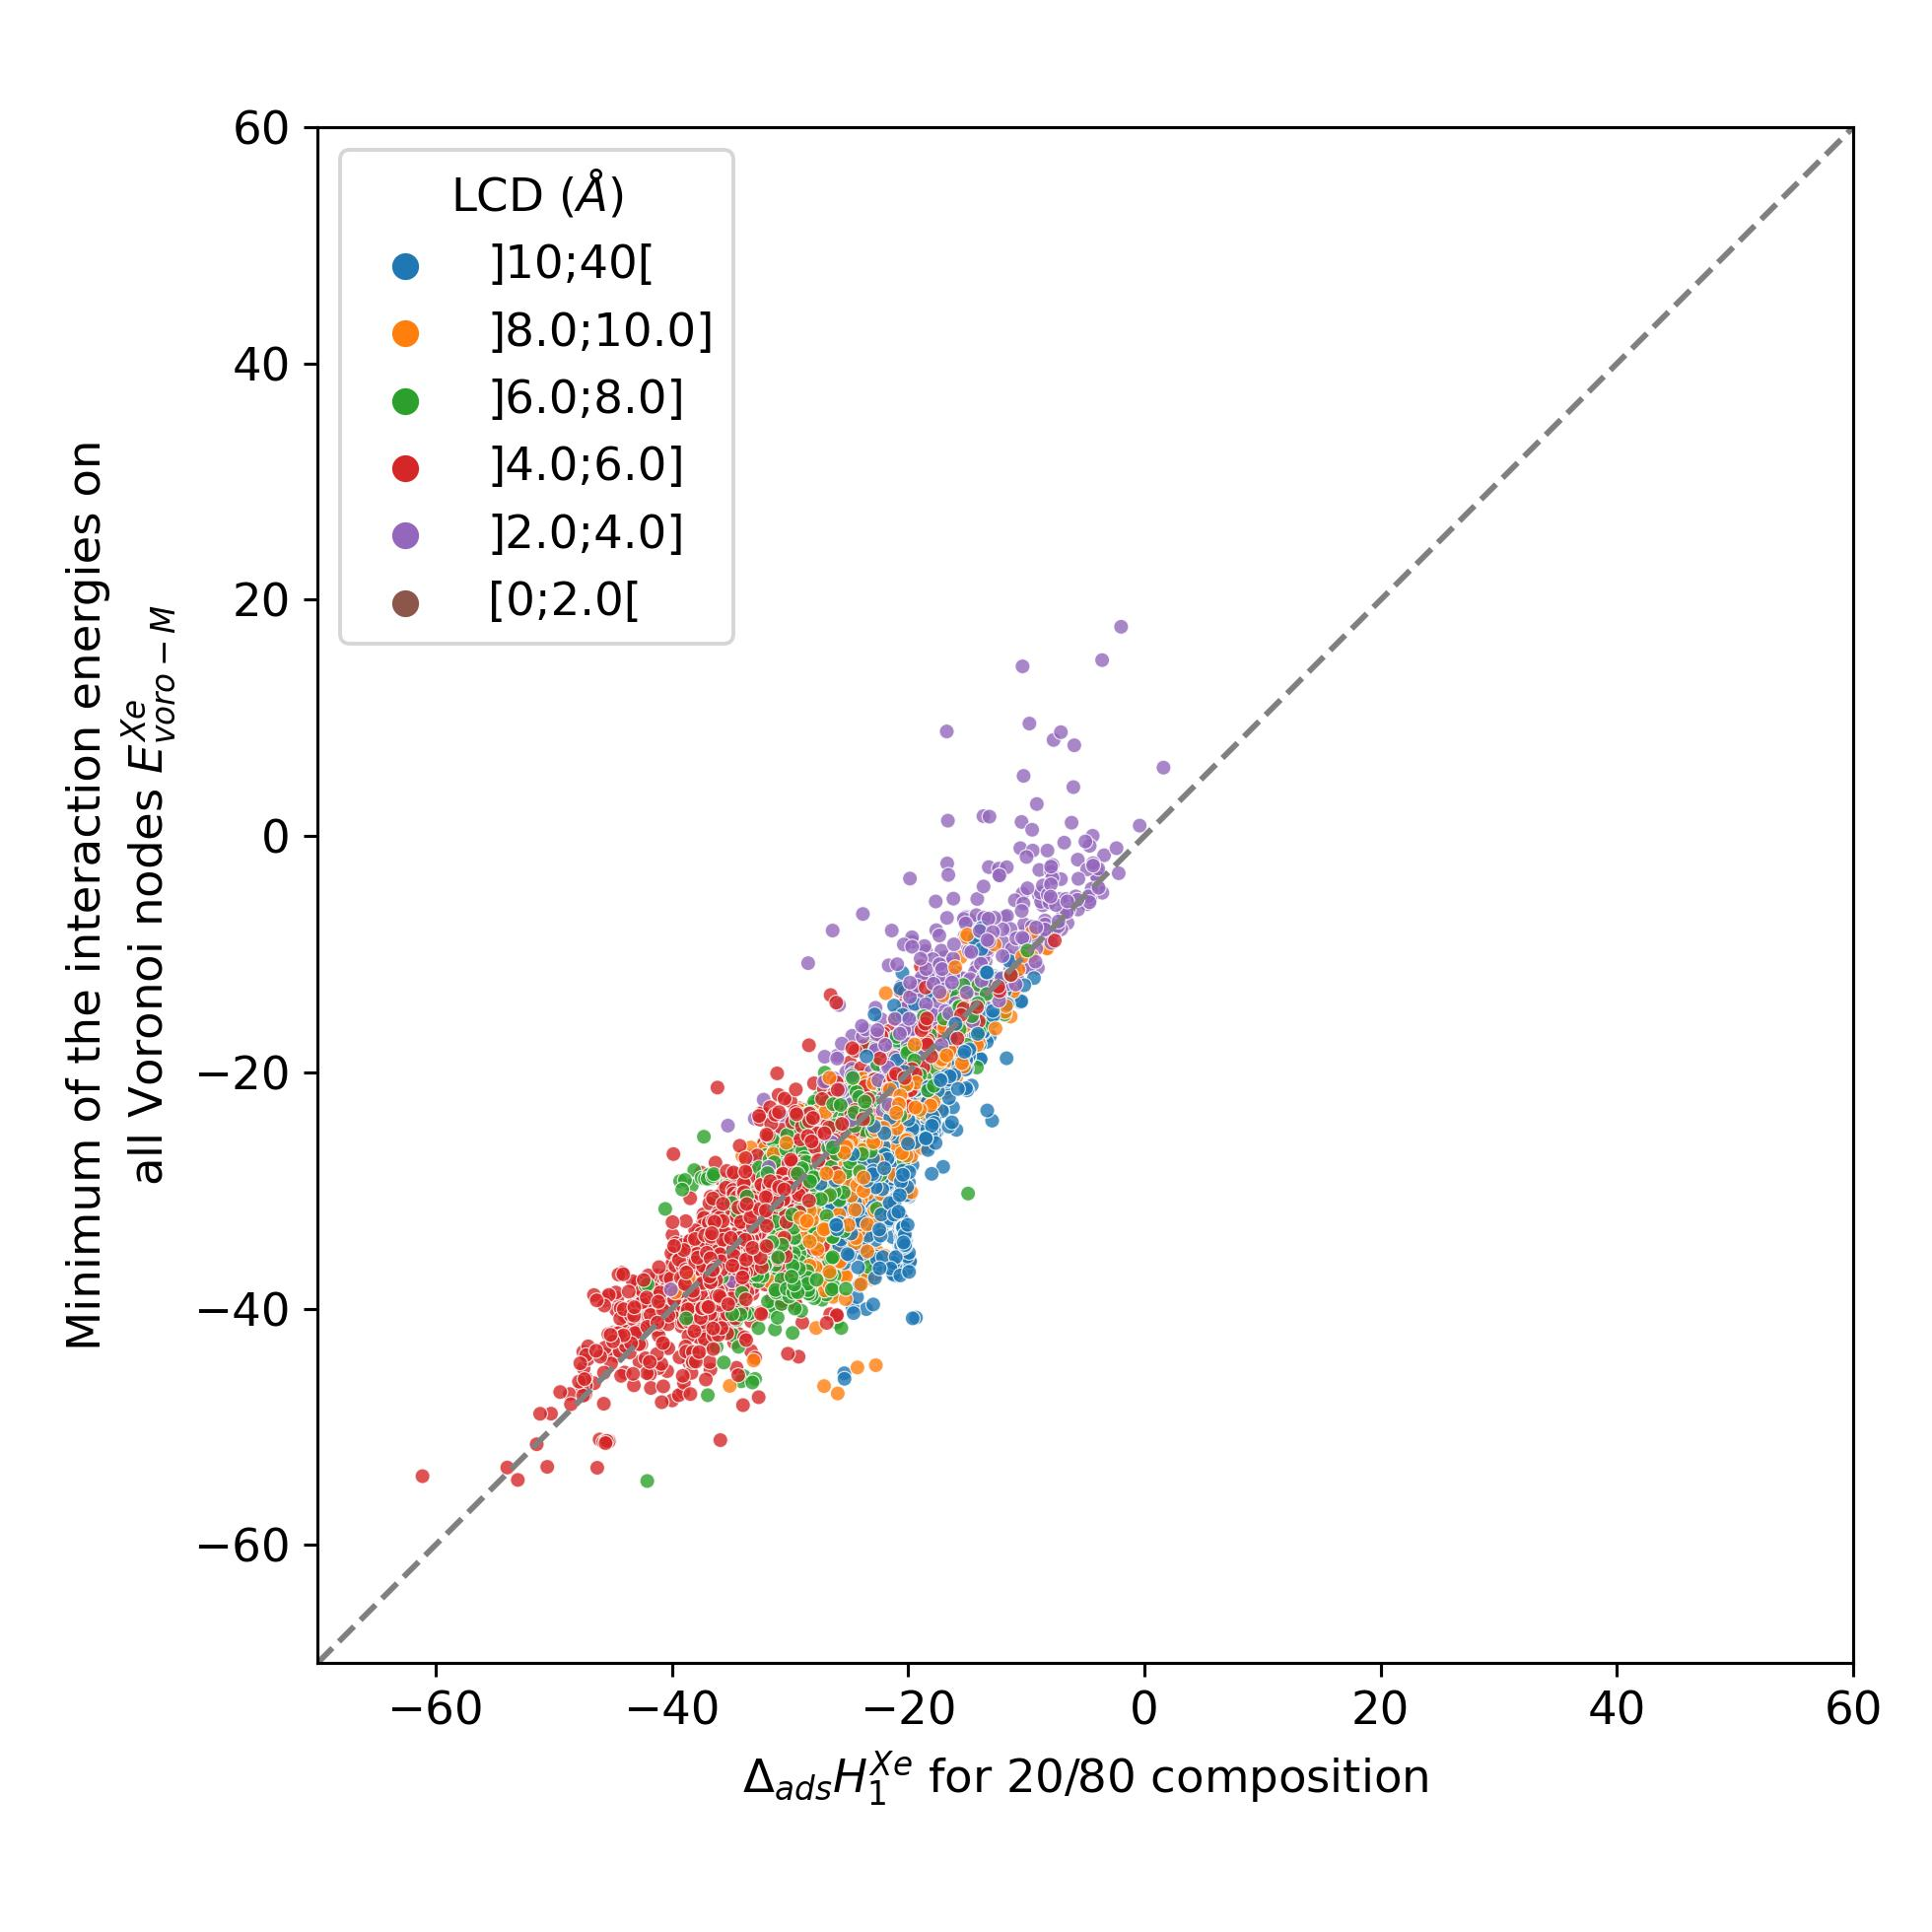
\includegraphics[width=0.32\textwidth]{figures/3-fastsim/H_Xe_2080_vs_E_voro_M_overview.jpg}
      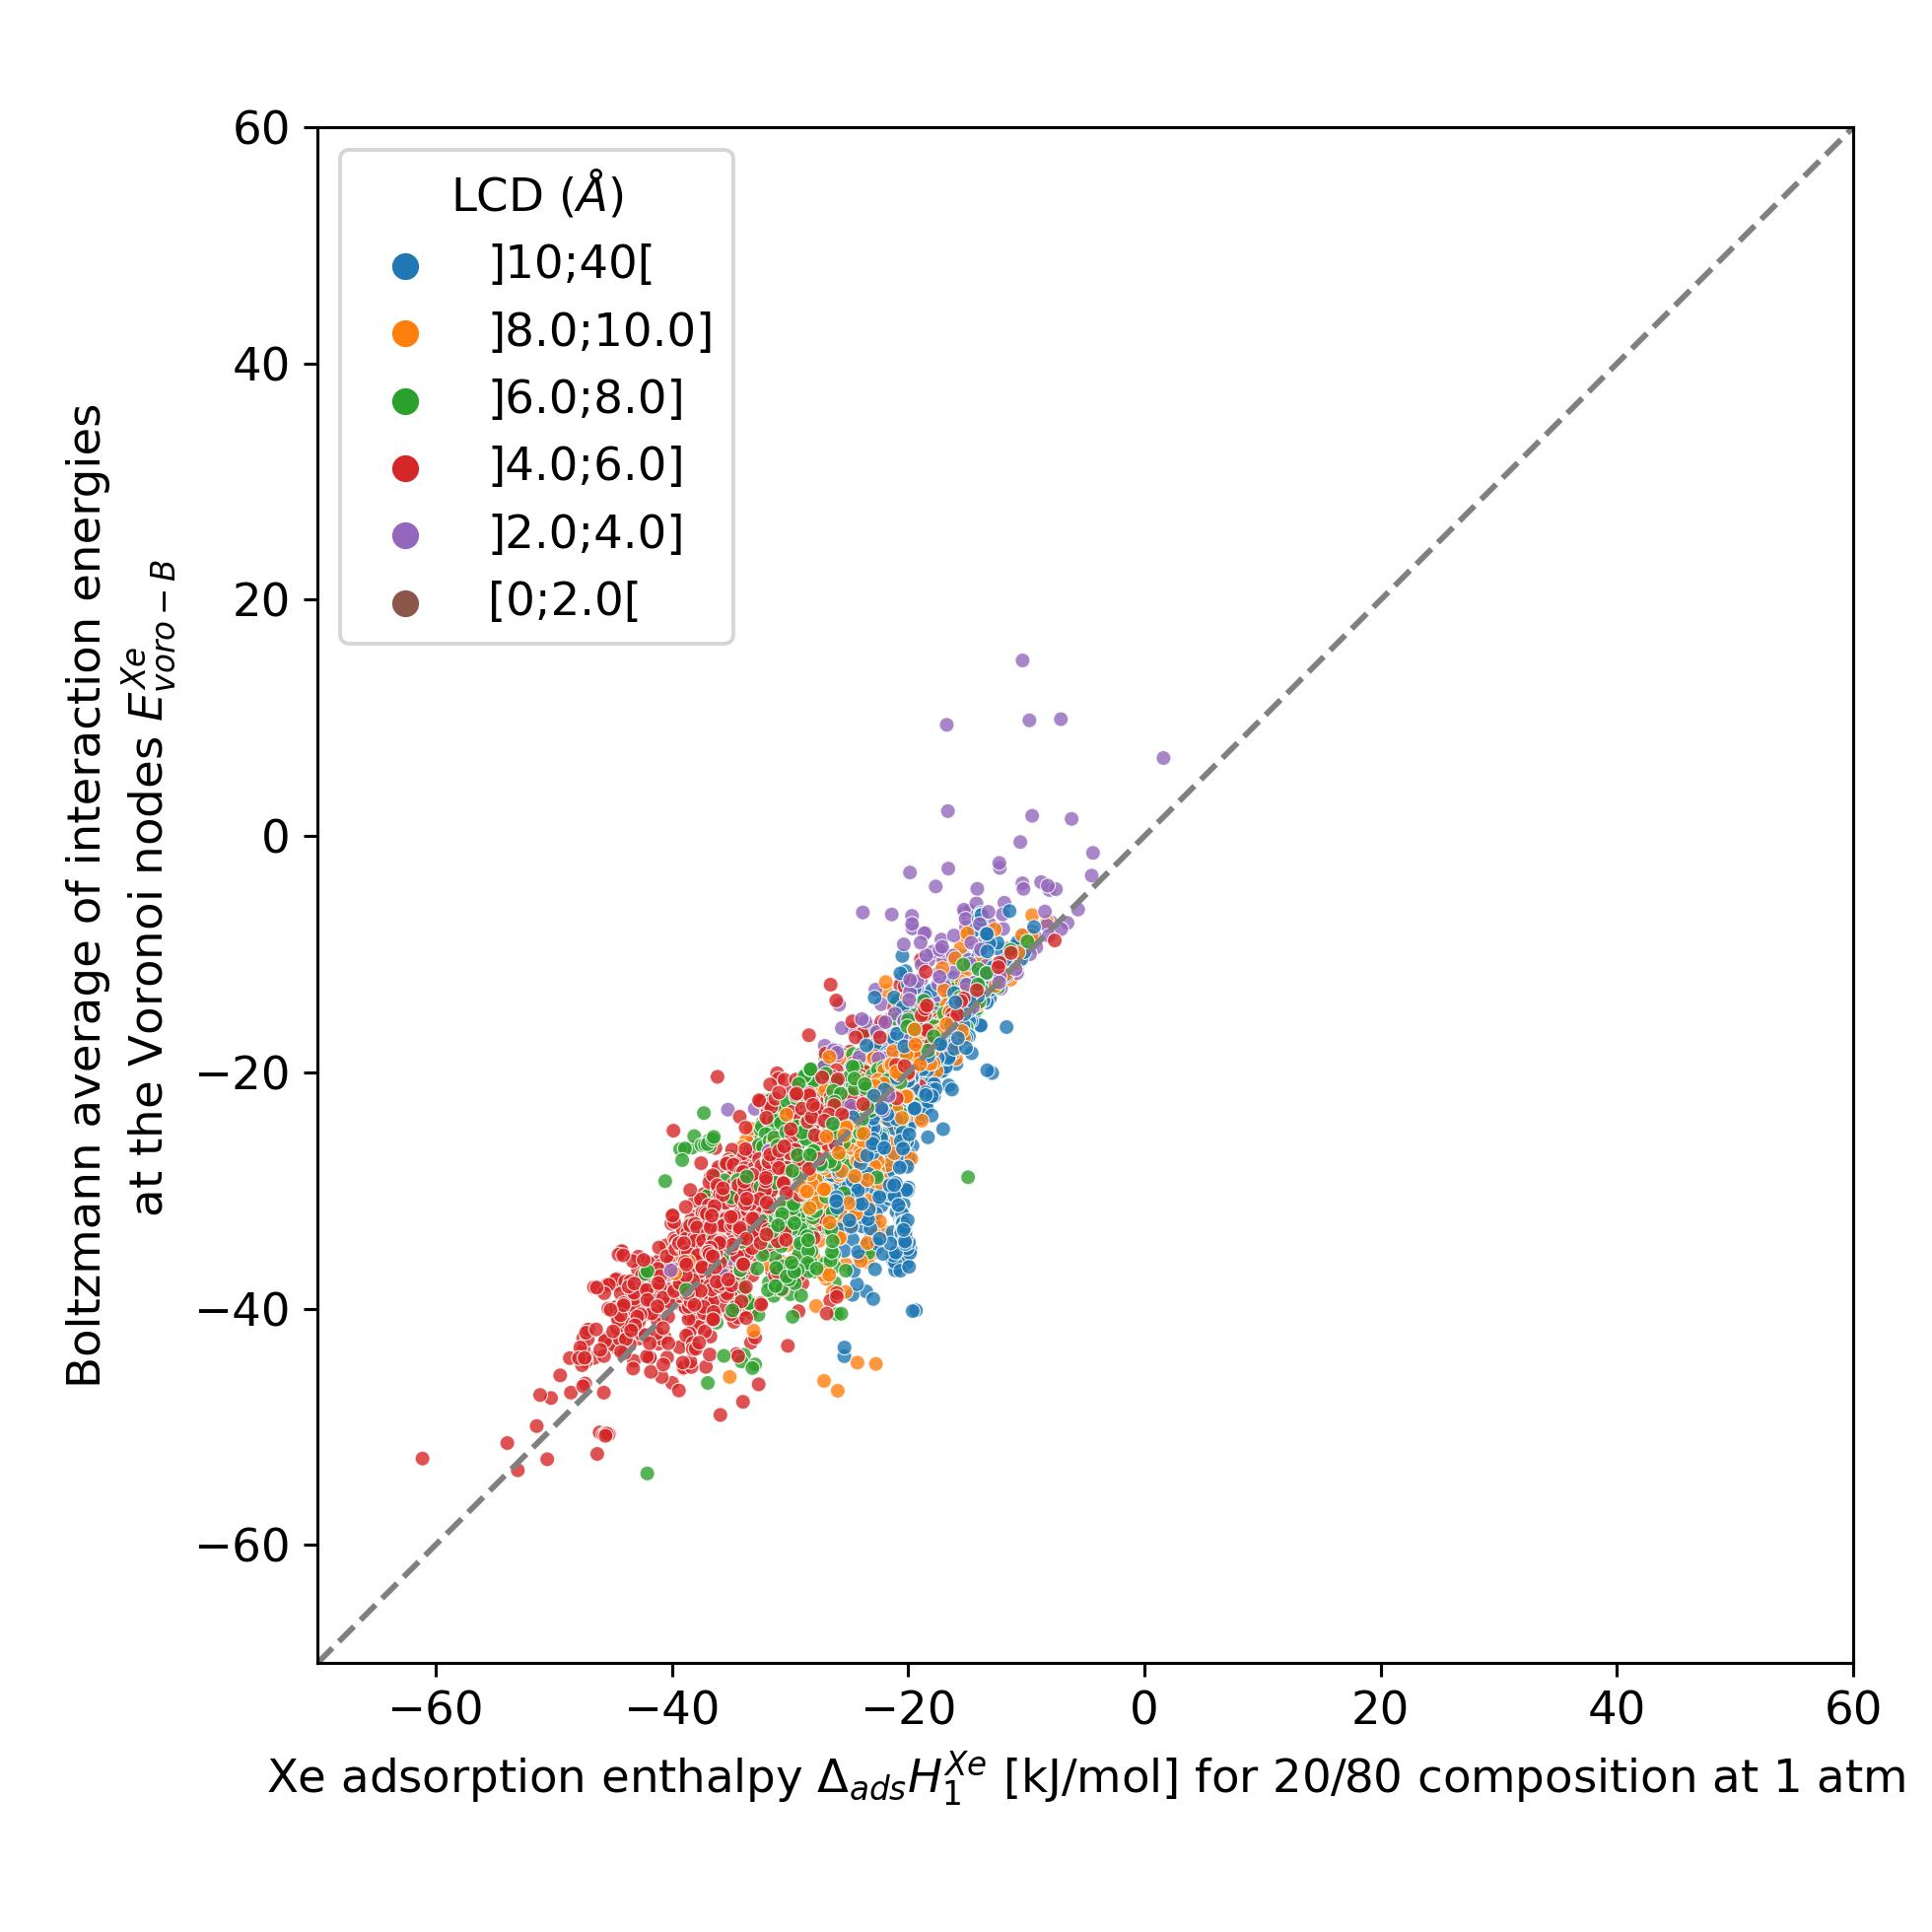
\includegraphics[width=0.32\textwidth]{figures/3-fastsim/H_Xe_2080_vs_E_voro_B_overview.jpg}
      \caption{Scatterplots of the energy descriptors $E\e{voro-A}^{Xe}$, $E\e{voro-M}^{Xe}$ and $E\e{voro-B}^{Xe}$ calculated by a Voronoi sampling compared to the enthalpies calculated by a 100k-step GCMC simulation of xenon in structures of CoRE MOF 2019. The points are labeled according to the largest cavity diameter (LCD\e{CCDC} or $D_i$) belonging to one of the intervals.}\label{fgr:compa_voro_2080}
  \end{figure}
  
At higher pressure, the adsorption enthalpy has higher values, resulting in a diminished correlation between the Boltzmann average and the minimum of the interaction energies calculated at the Voronoi nodes. The regular averaging approach tends to overestimate the energy values, bringing them closer to the values observed at higher pressures. To address this issue, an alternative averaging method that assigns greater weights to the higher energy values has been developed. This new approach resembles a Boltzmann average with a higher temperature value. The next chapter will focus on testing and evaluating the performance of this alternative method. The overestimation of energy values in the averaging process allows these values to align more closely with the ones observed at higher pressures. Drawing inspiration from this idea, an alternative averaging method that assigns greater weights on the higher values has been developed in this thesis. This modified Boltzmann average with increased weights for higher energy values will also be tested in the next chapter.

\subsection{Performance of a Voronoi energy sampling}

This section will focus on some performance metrics associated with the Boltzmann average at the Voronoi nodes and comparison with the reference sampling method, the Widom insertion with 100,000 cycles. The right plot of the Figure~\ref{fgr:compa_voro_0} compares the enthalpy computed in the Voronoi sampling with the reference adsorption enthalpy (ground truth) --- showing at the same time the largest cavity diameter for each porous framework. The correlation between the values of enthalpy is found to be strong for only a limited number of structures with enthalpy around \SI{-50}{\kilo\joule\per\mole}. For structures with higher enthalpy, the correlation diminishes, particularly for structures with small-pore sizes. For the points in purple, the largest cavity diameter is lower than the kinetic diameter of a xenon, and the Voronoi node sampling is clearly deemed insufficient. In addition, the loss of accuracy observed for other points (larger pores) can be explained by the fact that the pores are slightly larger and the center of the pore is no longer an accurate approximation of the adsorption site position, as the adsorption sites are closer to the pore surface than the center of the pore. Consequently, these findings have motivated the proposal of a new sampling scheme based on the molecular surface of the pore space, which will be elaborated in subsequent sections.

Evaluating the performance metrics, the root mean squared error (RMSE) {and the mean absolute error (MAE) for Voronoi sampling are determined to be \SI{6.78}{\kilo\joule\per\mole} and \SI{2.01}{\kilo\joule\per\mole}} respectively, when considering all structures in the set. These values appear to be too high to be used for screening purposes. However, non-porous materials would be screened out \emph{a priori} in any high-throughput workflow due to their lack of relevance. Therefore, the focus can be placed on structures with cavities larger than \SI{3.7}{\angstrom} (slightly lower than \SI{3.96}{\angstrom} Xe kinetic diameter). By restricting the analysis to such structures, {the RMSE and MAE decrease to \SI{2.11}{\kilo\joule\per\mole} and \SI{1.55}{\kilo\joule\per\mole} respectively}. These values can be considered acceptable for a rapid estimation of the guest--host affinity, although they are not suitable for accurate adsorption enthalpy calculations.

The low computational cost of the method further supports its feasibility. The Voronoi tessellation performed by the Zeo++ software is extremely fast, generating the positions of the Voronoi nodes in approximately \SI{0.28}{\second} (on average across all the structures of the CoRE MOF 2019 database), using a typical workstation (a single Intel Xeon Platinum 8168 core at 2.7~\si{\giga\hertz}). In comparison, a simple Python for energy calculation required around \SI{27}{\second} per structure, whereas an optimized C++ implementation benchmarked in this thesis achieved Voronoi sampling in approximately \SI{0.4}{\second}. Consequently, the Voronoi sampling method requires only a few hundred milliseconds per structure, whereas a Widom insertion method necessitates approximately hundreds of seconds per structure. Thus, Voronoi sampling exhibits computational efficiency that is 2 to 3 orders of magnitude higher than that of a full sampling of the pore space.

This preliminary study has identified a fast method for adsorption enthalpy calculation that can be widely used in screening procedures. However, its accuracy for quantitative prediction is limited --- this sampling technique assumes that the nodes are close to the real, most favorable adsorption sites, which may not always hold true. Specifically, the assumption that the adsorption sites must be located at the center of the pores is only valid for structures with pore sizes close to the size of the adsorbate. This observation raises key questions regarding the importance of selecting appropriate sampling points within the pore space of materials. Consequently, an intermediate technique was developed and optimized to address these limitations and provide a sampling approach that is both fast and accurate for predicting adsorption enthalpy. This new technique focuses the sampling on the surface of the material, aiming to compensate for the primary flaws encountered in the Voronoi sampling approach.

\section{Rapid Adsorption Enthalpy Surface Sampling (RAESS)}\label{sct:RAESS}

In this section, the development of our surface sampling algorithm will be described, aiming to achieve higher accuracy than Voronoi sampling and greater efficiency than Widom insertion. The initial idea is based on a series of theoretical considerations: (i) strong adsorption sites are located near the surface of the material; (ii) by changing the problem from 3D to 2D sampling, the complexity can be reduced; and (iii) the algorithm can scale with the number of unique atoms in the structure (rather than the size of the unit cell), which is efficient as many porous frameworks exhibit high symmetry. The first physical intuition ensures that the proposed method will yield more accurate results compared to Voronoi sampling, while the latter two considerations enable more efficient sampling, resulting in faster execution for a well-optimized code. To validate these hypotheses, an analysis of both the accuracy and speed of the new algorithm will be conducted and compared against existing methods. It is worth noting that the study described in this section has already been published in the Chemical Science journal~\cite{Ren_2022}.

\subsection{Initial implementation}

The initial implementation of the surface sampling algorithm and its principles are presented in this section. Although this initial implementation is relatively basic, it already demonstrates good performance compared to other methods. In subsequent sections, further refinements will be made through the introduction two additional features that will improve both the accuracy and speed of the algorithm.

This initial implementation accelerates the calculation of adsorption enthalpy in nanoporous materials by sampling interaction energies exclusively near the surface. Figure~\ref{fgr:principle} provides an illustration of this approach. To achieve this, a loop is performed over all unique atoms (as defined by crystalline symmetry). For each atom, a sphere is sampled around its position using a uniform distribution. These sampled points, referred to as sampling points, can be adjusted in number. The default radius for the sampling spheres is set to the distance $r\e{min}=2^{1/6}\sigma_{ij}$, which corresponds to the minimum of the LJ potential between atoms of type $i$ (belonging to the framework) and $j$ (the guest). This choice represents the strongest possible pair interaction (although the neighboring atoms will obviously have an influence). After calculating the interaction energy at each sampled point, a Boltzmann average of these energies is obtained. This average corresponds to a biased adsorption enthalpy, as described by the equation~\ref{eq:ads_enthalpy}.

\begin{figure}[ht]
\centering

  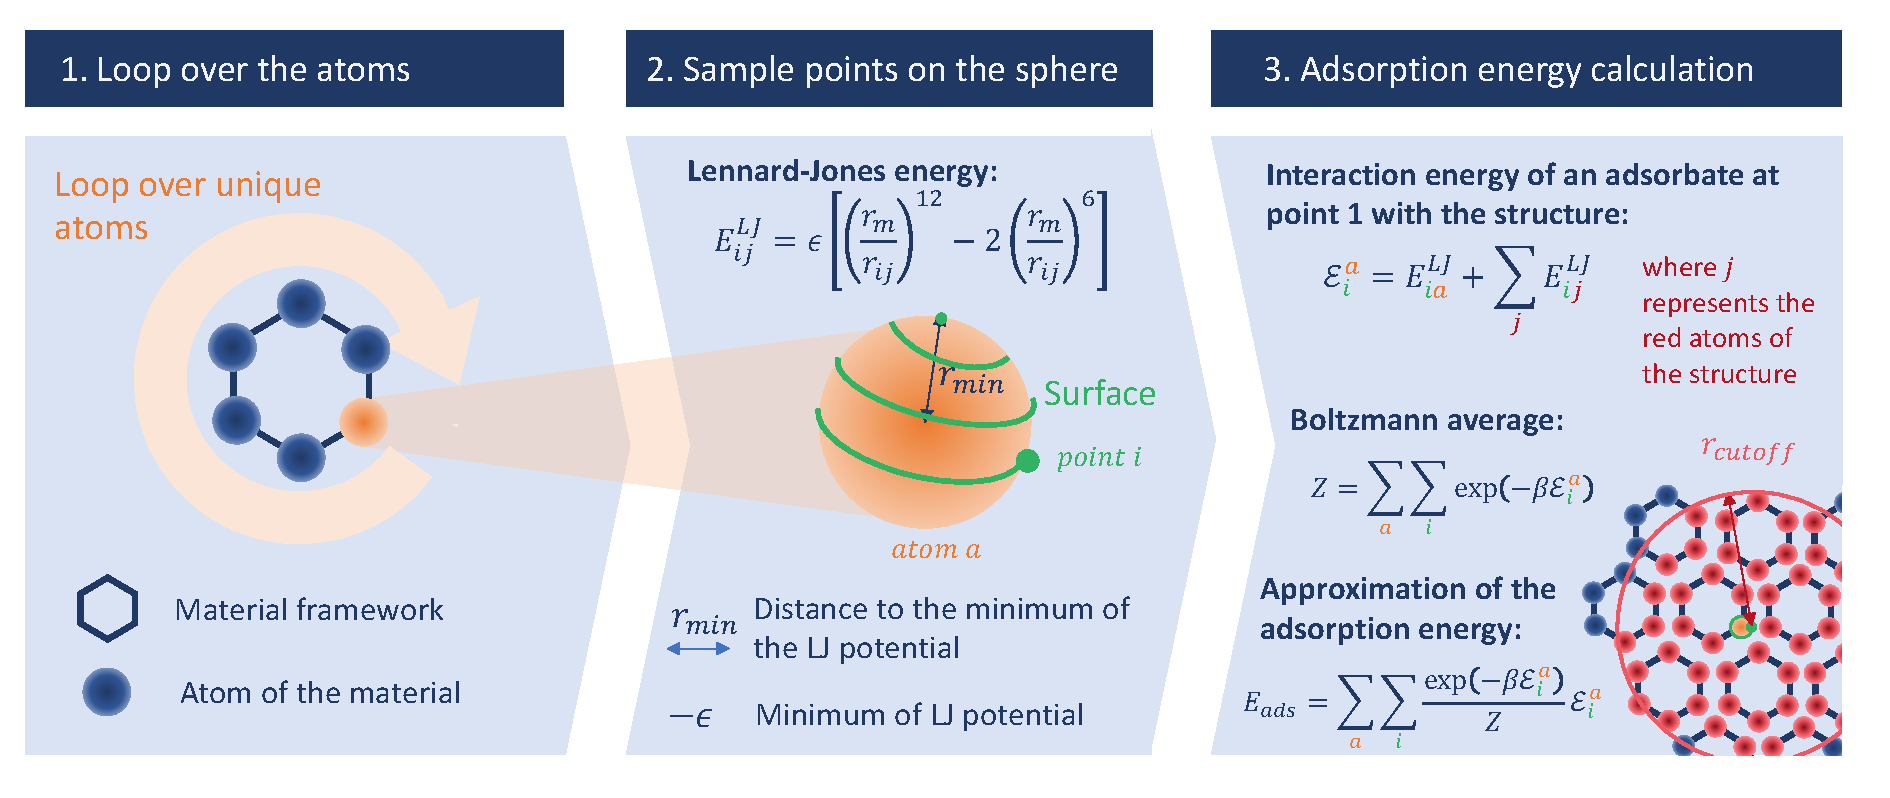
\includegraphics[clip, trim=0.6cm 0.74cm 0.78cm 0.6cm,width=0.95\linewidth]{figures/3-fastsim/Principe_screening.pdf}
  \caption{Schematic description of the surface sampling based on the three main steps of the algorithm: the loop over the unique atoms, the spiral sampling around each atom, and the energy averaging. The adsorbate is represented by the point $i$ and is moved across all the points around the unique atoms of the structure.}\label{fgr:principle}
\end{figure}

To validate the accuracy of the approximation made using this sampling, the algorithm was applied with 300,000 sampling points per unique atom. The results, as illustrated by Figure~\ref{fgr:surface_sampling}, demonstrate a good numerical agreement with the reference calculations, {the RMSE and MAE being found to be only around \SI{0.90}{\kilo\joule\per\mole} and \SI{0.66}{\kilo\joule\per\mole} respectively}, considering all the structures from the database. Moreover, no noticeable difference in RMSE was observed when considering the structures with a pore size above \SI{3.7}{\angstrom} (as determined by the LCD\e{CCDC}). Unlike Voronoi sampling, this method provides consistent accuracy across all the structures of the database, with a lower error. The validation of an {RMSE} value below \SI{1}{\kilo\joule\per\mole} supports the intuition that this new sampling technique achieves a balance between the accuracy and efficiency of the previously introduced methods (Voronoi and Widom).

\begin{figure}[ht]
  \centering
  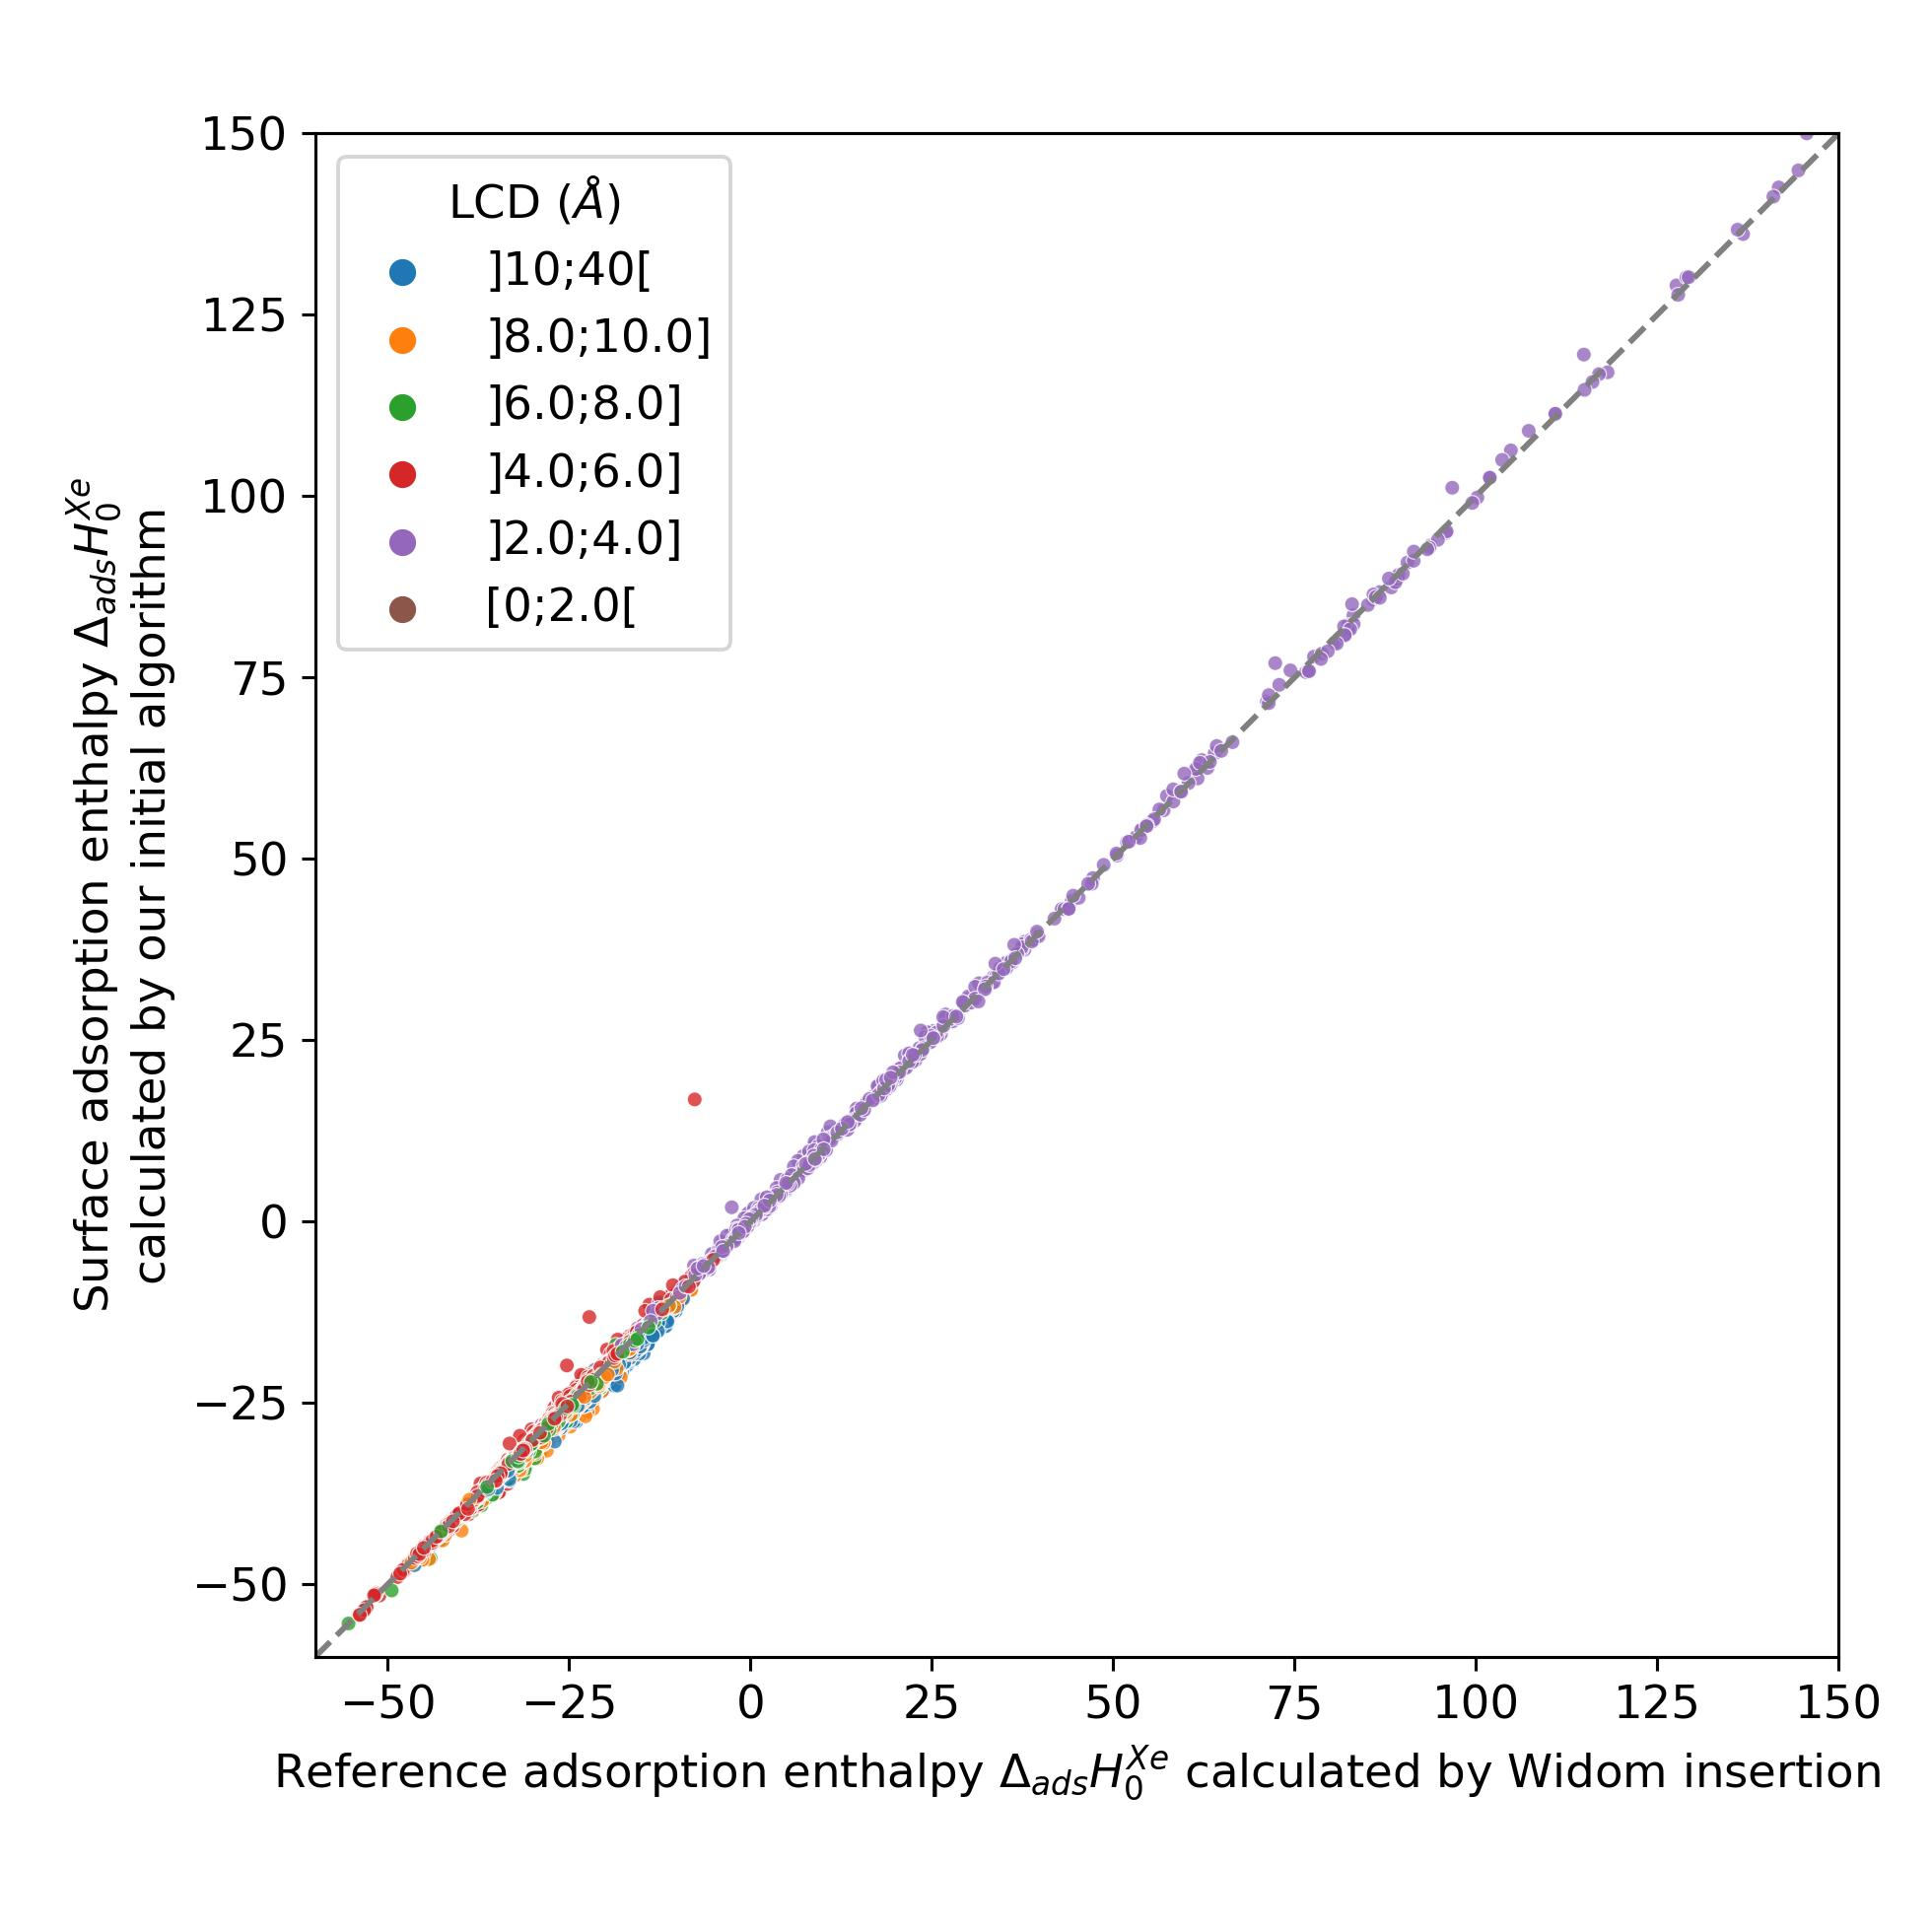
\includegraphics[width=0.45\linewidth]{figures/3-fastsim/H_Xe_widom_vs_H_Xe_surface_spiral_overview.jpg}
  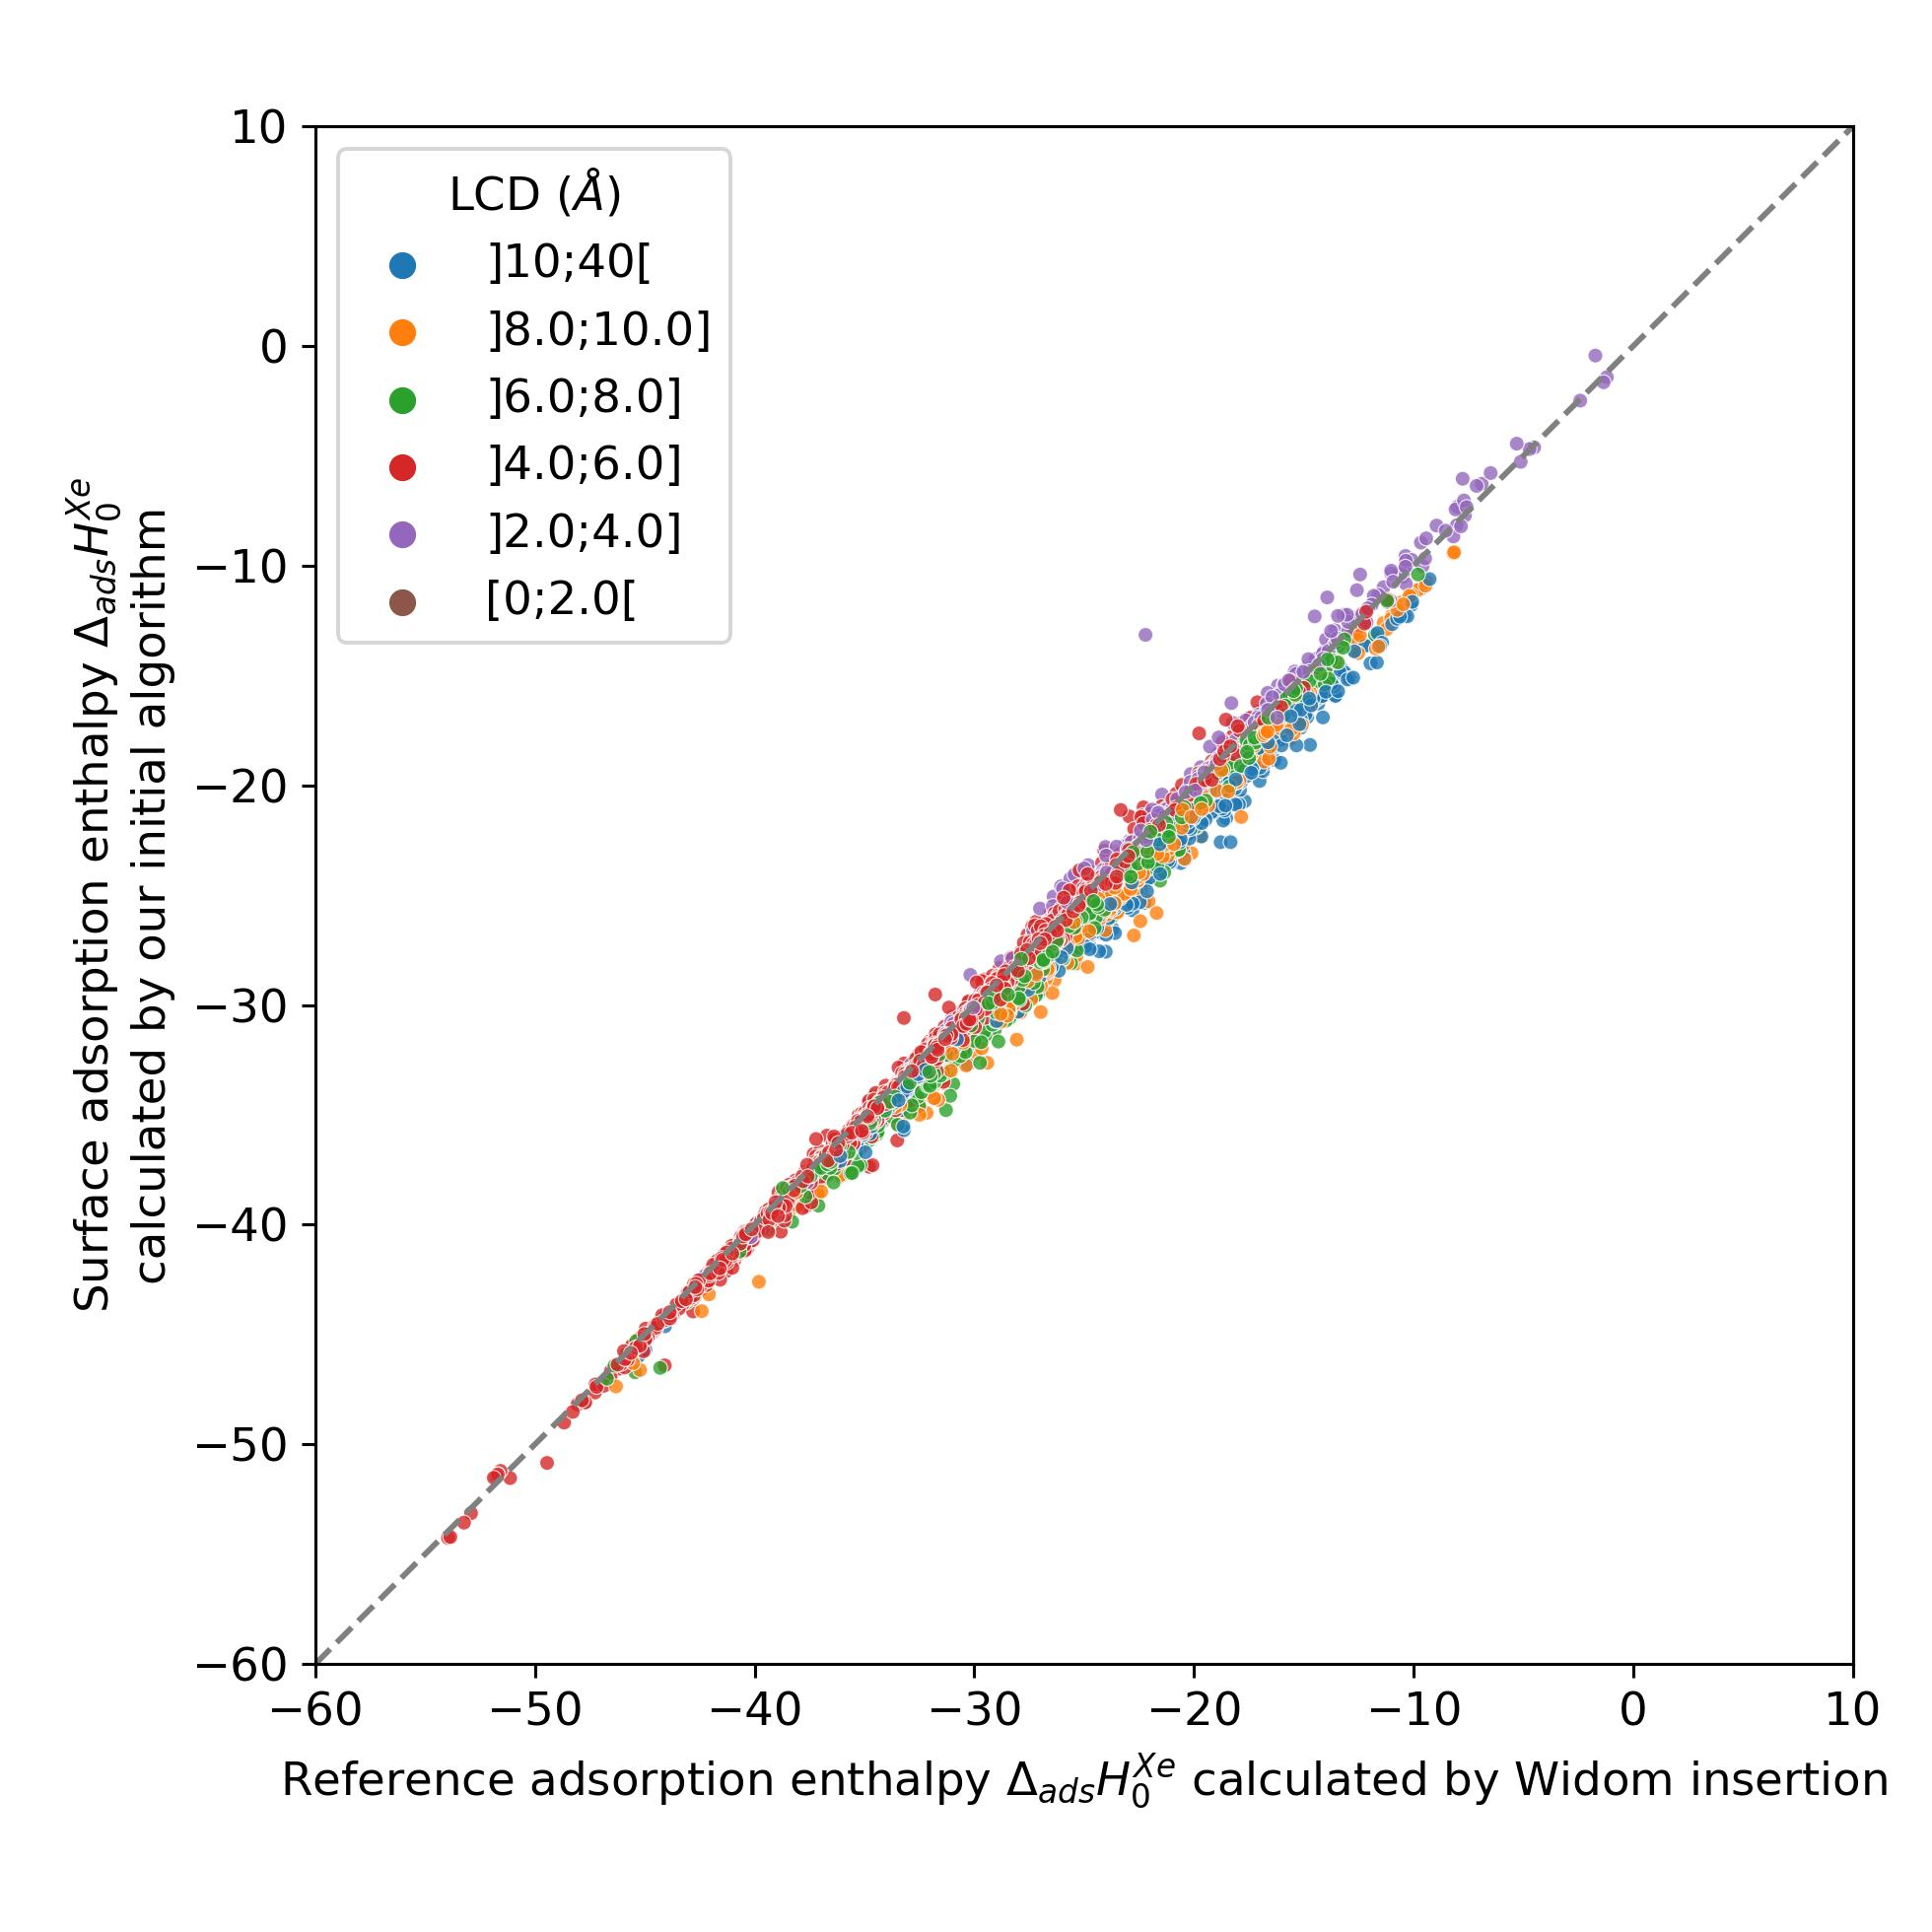
\includegraphics[width=0.45\linewidth]{figures/3-fastsim/H_Xe_widom_vs_H_Xe_surface_spiral_zoom.jpg}
    \caption{Scatterplots of the xenon surface adsorption enthalpy calculated by an initial implementation of the RAESS algorithm as a function of the xenon adsorption enthalpy calculated by a 100k-step Widom insertion simulation using two value windows. The second plot zooms on the negative values corresponding to the most selective materials.}\label{fgr:surface_sampling_init}
\end{figure}

After proving its good accuracy, the computation time required for the method was explored. Figure~\ref{fgr:convergence} illustrates that the method reaches an RMSE below \SI{1.0}{\kilo\joule\per\mole} promptly, with an average CPU time of \SI{1.2}{\second}, corresponding to 2,000 sampling points per atom. This is signficantly shorter than the \SI{150}{\second} required for a Widom insertion to approach its plateau value (converging to zero), with an RMSE of \SI{0.10}{\kilo\joule\per\mole} and 12,000 cycles. Additionally, the Widom insertion takes approximately \SI{14}{\second} to achieve a similar RMSE of \SI{1.0}{\kilo\joule\per\mole}, which is still slower than the surface sampling. Therefore, this initial implementation of surface sampling exhibits faster computation time than a standard Widom insertion, while maintaining good accuracy.

The observed convergence speed and limit values of the error can be explained by the nature of each sampling method. In surface sampling, the sampled points are biased towards the most attractive adsorption points for xenon, leading to a rapid convergence since the most influential terms of the Boltzmann average are quickly gathered. On the other hand, in a Widom insertion, every point in space has an equal chance of being sampled, which closely aligns with the definition of enthalpy but requires much more time to randomly sample highly attractive adsorption sites. However, due to its biased nature, surface sampling is inherently less accurate, as not all points are considered equally, potentially missing the most optimal adsorption site in some cases, especially if it is located further from the sampled surface.

\begin{figure}[ht]
  \centering
    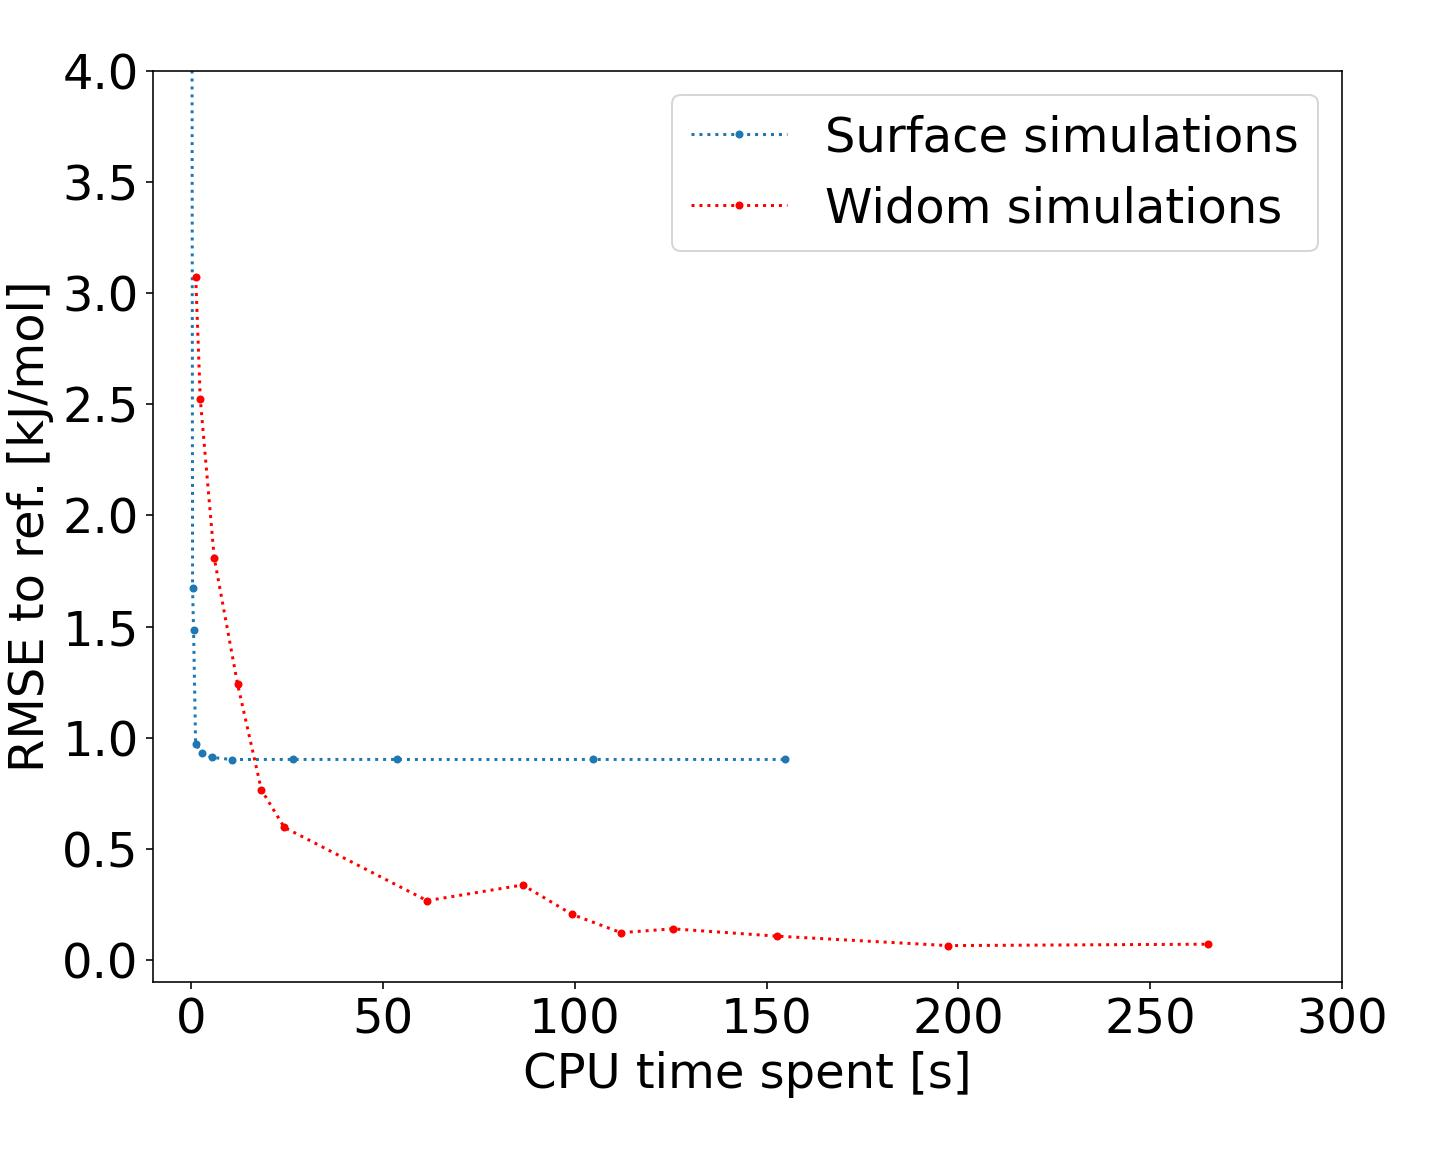
\includegraphics[width=0.7\linewidth]{figures/3-fastsim/time_rmse.jpeg}
    \caption{Convergence plot of the RMSE on the adsorption enthalpy for the RAESS algorithm (blue) compared to a 100k-step Widom insertion simulation (red) for xenon adsorption in {all} structures of the CoRE MOF 2019 database.}\label{fgr:convergence}
  \end{figure}
  

However, this initial implementation of the method is slower than a Voronoi sampling, which only requires an average of around 1,600 sampled points, as opposed to approximatley 13,000 sampled points on average (when multiplied by the average number of unique atoms). The sampling process would take approximately \SI{0.15}{\second}, while the generation of Voronoi nodes would take about \SI{0.28}{\second}, resulting in the surface sampling algorithm being 2 to 3 times slower (both methods implemented in an identical compiled language, in this case C++). To improve both the accuracy and performance, further adjustments were made to the surface sampling method. The size of the sampling sphere was adjusted, and a fast rejection criterion was implemented. The rejection of high-energy points with little contribution to the final enthalpy value helps reduce simulation time, while the size of the sampling sphere can improve accuracy. As the initially chosen sphere size considered only the interaction with the closest atom, the size was set at the minimum of the Lennard-Jones potential. However, taking into account the interaction with neighboring atoms can further stabilize the adsorbate, and sampling beyond this minimum can potentially increase the accuracy of the surface sampling method.

\subsection{Performance improvement of the algorithm}

\subsubsection{Size of the sampling sphere}

The validity of the initial algorithm is based on the assumption that the adsorption site corresponds to the minimum of the Lennard-Jones potential. This assumption holds true when the closest atom contributes significantly to the overall interaction. However, in real frameworks, other neighboring atoms also contribute to the host/guest interaction, and in most materials, the adsorption sites are found to be often located farther apart than the LJ potential minimum to maximize the contribution of all atoms --- the dissymmetry of the interaction potential well further supports this observation. To explore the possibility of incorporating this insight into the RAESS algorithm, a parameter $\lambda$ was introduced, and the sampling sphere radius was defined by $R_{\lambda} = \lambda \sigma$, where $\sigma$ represents the distance at which the LJ potential is zero. If $\lambda=2^{1/6}$, the algorithm reverts to the initial definition of the sampling sphere, where the adsorbent is situated at the minimum of the LJ potential for the atom. For $\lambda=1$, the sampling sphere is centered at the zero of the LJ potential. By varying this parameter, this intuition regarding the optimal positioning of the sampling sphere can be examined and validated.

\begin{figure}[ht]
\centering
  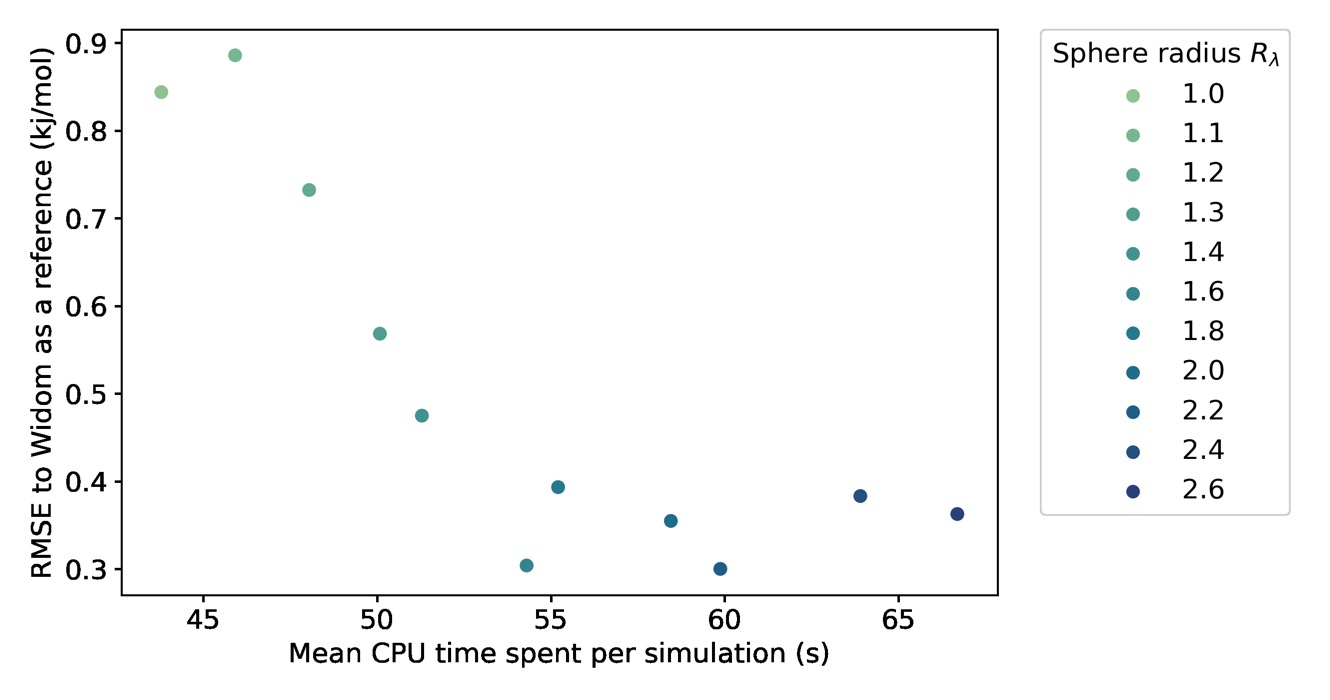
\includegraphics[width=0.7\linewidth]{figures/3-fastsim/sphere_size_optimisation.jpg}
  \caption{Influence of the sampling sphere radius $R_{\lambda}$ on the average CPU time required for a simulation of 100k sampling points and the RMSE, compared to the reference adsorption enthalpy. The averaging is done only on the structures with the largest cavity diameter (LCD\e{CCDC}) higher than \SI{3.7}{\angstrom}.}\label{fgr:radius}
\end{figure}

As no analytical model could determine the optimal value for the sampling sphere, a statistical approach was adopted to study the influence of the $\lambda$ parameter on both the accuracy and computation time. The results are presented in Figure~\ref{fgr:radius}. It was observed that the RMSE is relatively high, around \SI{0.90}{\kilo\joule\per\mole}, for radius sphere lower than the $r\e{min}$, and then decreases to reach a plateau around \SI{0.35}{\kilo\joule\per\mole}, as the radius increases. This confirms that increasing the sampling sphere radius can enhance the accuracy of the algorithm, and it was found that values of $\lambda$ higher than $1.6$ lead to the accuracy stabilized accuracy. This study also found that increasing the sphere radius negatively impacts computational efficiency, as it involves considering a larger number of neighboring atoms in the energy calculation.

By choosing an optimal sampling sphere, it is possible to reduce the error by more than half while increasing the computation time by approximately 20 percent when comparing $\lambda=1.6$ with $\lambda=1.1$ (close to $r\e{min}$). In most cases, this trade-off is acceptable. However, in scenarios where computation time is crucial, such as rapid screening, the optimal choice might not be to increase the sampling sphere at $\lambda=1.6$ but to choose a lower sampling sphere radius at $\lambda=1.4$ or $\lambda=1.2$, resulting in an RMSE around \SI{0.5}{\kilo\joule\per\mole} --- still considered quite acceptable. The introduction of the new scale parameter in this section allows users to tailor the algorithm according to their specific purposes, prioritizing either accuracy or computation speed. {If the method is applied to a completely different database under different conditions, users can choose a default value that works well, such as (\emph{e.g.} $\lambda=1.4$), or optimize the parameter based on a small diverse sample of the unseen data.}

\subsubsection{Rejection condition}\label{sct:rejection_condition}

As demonstrated above, the RAESS algorithm exhibits improved accuracy compared to Voronoi sampling. However, its initial implementation was significantly slower, which could hinder its applicability in high-throughput screening workflows involving large numbers of structures, potentially exceeding one million. To address this computational expense, this thesis implemented a mechanism to reject points with minimal contribution to the final enthalpy i.e. the exlusion of sampling points that yield largely positive interaction energies, as these would have negligible impact when exponentiated in the Boltzmann average calculation.

\begin{figure}[ht]
\centering
  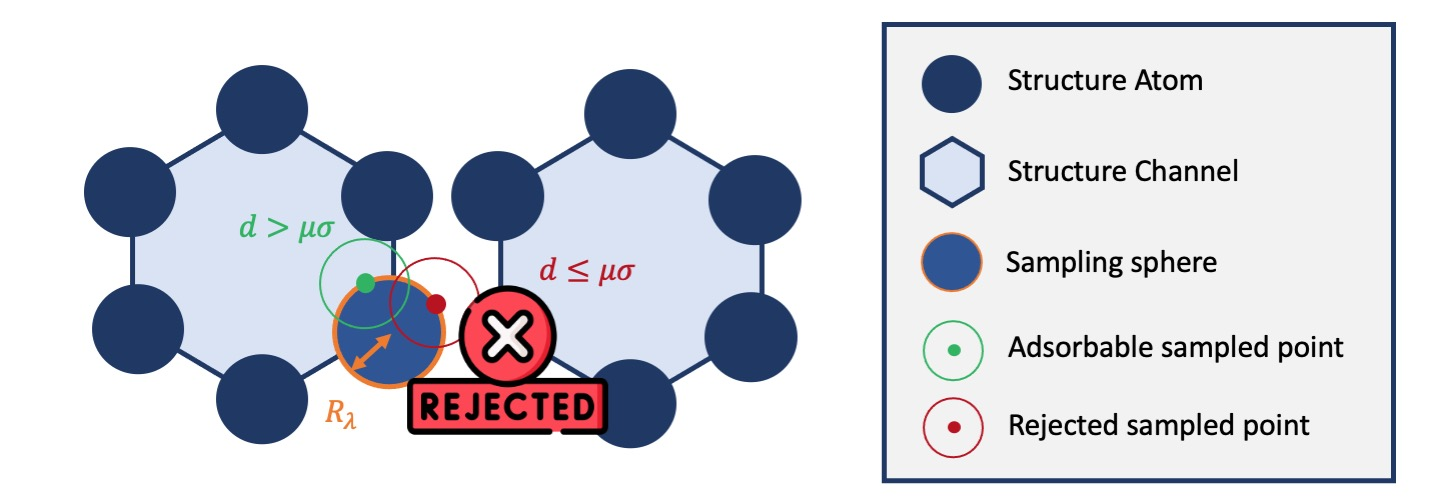
\includegraphics[width=\linewidth]{figures/3-fastsim/rejection_sampling_sphere.jpg}
  \caption{Simplified representation of the principle of rejection condition and the concept of sampling sphere inside 2D channels of a nanoporous material.}\label{fgr:feature}
\end{figure}

Inspired by conventional methods for calculating accessible surface, a hard sphere rejection condition based on the distance to neighbors was implemented. If the adsorbate is too close to another atom of the structure, the sampling point is rejected, i.e., its energy is not calculated (or considered to be infinite). The distance threshold is based on the $\sigma_{ij}$ parameter of the Lennard-Jones potential. To determine the optimal threshold, a factor $\mu$ with real values between 0 and 1 was introduced, which modifies the size of the hard sphere rejection condition. If the guest--host distance is lower than $d_{\mu} = \mu \times \sigma$, the point is rejected. The absence of a rejection condition occurs when $\mu = 0$, while a value of $\mu = 1$ leads to the rejection of all points with a positive energy interaction with at least one atom of the structure. However, this condition may be overly stringent, resulting in the rejection of points with non-negligible contributions. The rejection condition is schematically illustrated in Figure~\ref{fgr:feature}.

This rejection condition is expected to speed up the calculation process by avoiding energy computations for rejected sampling points. The energy calculation represents the largest proportion of the CPU time allocated to surface sampling. In the case of the \texttt{KAXQIL}\autocite{Banerjee_2012}, the Lennard-Jones potential calculation represents up to $90\%$ of the calculation time for 100,000 sampling points per sphere (using the initial algorithm). The number of rejections increases with higher values of the factor $\mu$. However, excessive rejections can adversely decrease the accuracy of the results. To strike a balance, a statistical analysis was performed to determine the optimal value of $\mu$, thereby enabling faster sampling without compromising the accuracy of the enthalpy calculation. The results of this analysis are depicted in Figure~\ref{fgr:rejection}.

\begin{figure}[ht]
\centering
  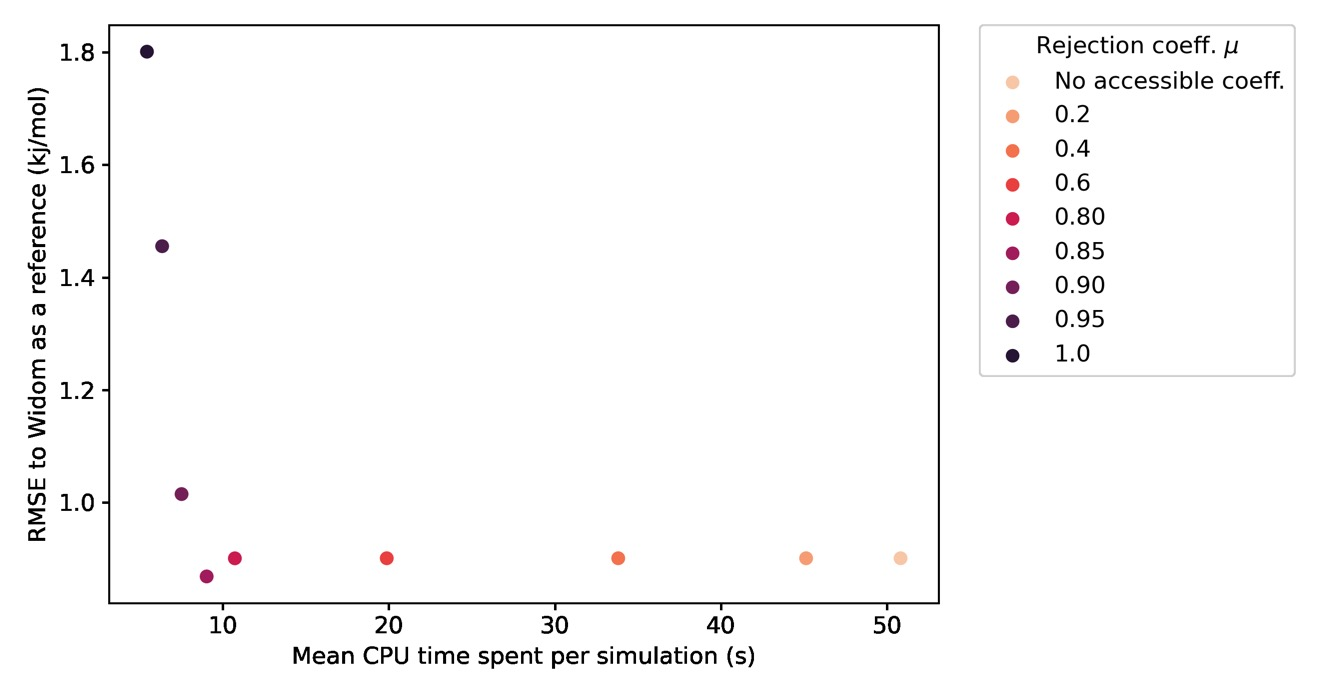
\includegraphics[width=0.7\linewidth]{figures/3-fastsim/rejection_coeff_optimisation.jpg}
  \caption{Influence of the rejection coefficient $\mu$ on the average CPU time required for a simulation of 100k sampling points and the RMSE compared to the reference adsorption enthalpy. The averaging is done only on the structures with the largest cavity diameter (LCD\e{CCDC}) superior to \SI{3.7}{\angstrom}. }\label{fgr:rejection}
\end{figure}

The values of RMSE and time presented in Figure~\ref{fgr:rejection} are averaged only for the most relevant structures regarding xenon adsorption (LCD\e{CCDC} $\geq$ \SI{3.7}{\angstrom}). For $\mu\leq 0.85$, an increase in the value of $\mu$ improves the computational speed without affecting the RMSE.\footnote{It should be noted that a decrease in accuracy is observed for structures with small pores due to the high probability of rejection within confined spaces, where all sampled points are ultimately rejected. However, these points are not considered when applying a filter on the cavity size (LCD\e{CCDC} $\geq$ \SI{3.7}{\angstrom}).} For high values of $\mu$, the rejection condition becomes overly stringent, leading to the rejection of points with non-negligible contribution to the overall enthalpy. The RMSE increases as a result. To maintain the same level of accuracy, the optimal value should be $\mu \simeq 0.85$, as it provides the lowest computation time with a similar RMSE. However, in specific cases, it may be feasible to explore higher values of $\mu$ that trade a slightly reduced accuracy for further gains in speed.

In the simulations depicted in Figure~\ref{fgr:rejection}, the use of a rejection condition $\mu = 0.85$ results in a four-fold acceleration of the simulation compared to the standard algorithm. In the following section, the combination of optimal values for the $\lambda$ and $\mu$ parameters generates an algorithm with highly favorable performance in comparison to Voronoi sampling or Widom insertion methods.

\subsection{Final surface sampling implementation}\label{sct:final_sampling}

\subsubsection{Performance comparison}

For the calculation of adsorption enthalpy, the proposed surface sampling method strikes a balance between the accuracy of Widom insertion (full sampling of the porous space), and the speed of less accurate methods such as Voronoi sampling. The performance of the algorithm, incorporating the two new features (sampling sphere scaling and rejection criterion) is illustrated in Figure~\ref{fgr:sumup}. This figure showcases the improvements brought about by each feature and provides a comparison with reference simulations. All CPU times are calculated using the possible minimum number of sampling points required for the respective algorithms to achieve convergence. With the implementation of the rejection condition, the surface sampling method is found to outperform Voronoi sampling in terms of computational speed. Moreover, increasing the size of the sampling sphere significantly enhances the accuracy of surface sampling, resulting in an RMSE of \SI{0.33}{\kilo\joule\per\mole} {and an MAE of \SI{0.21}{\kilo\joule\per\mole}}. For porous materials from the CoRE MOF 2019 database, the ideal set of parameters, $(\lambda = 1.6, \mu = 0.85)$, combines the lowest error and the smallest computational cost. By incorporating both of these new features into the algorithm, the final surface sampling method achieves an RMSE of only \SI{0.33}{\kilo\joule\per\mole} and an average computation time of \SI{0.34}{\second} per structure. According to the data represented in Figure~\ref{fgr:sumup}, this method is approximately 6 times more accurate and {$26$\%} faster than Voronoi sampling, and about 430 times faster than a Widom insertion with 12k cycles.

\begin{figure}[ht]
  \centering
  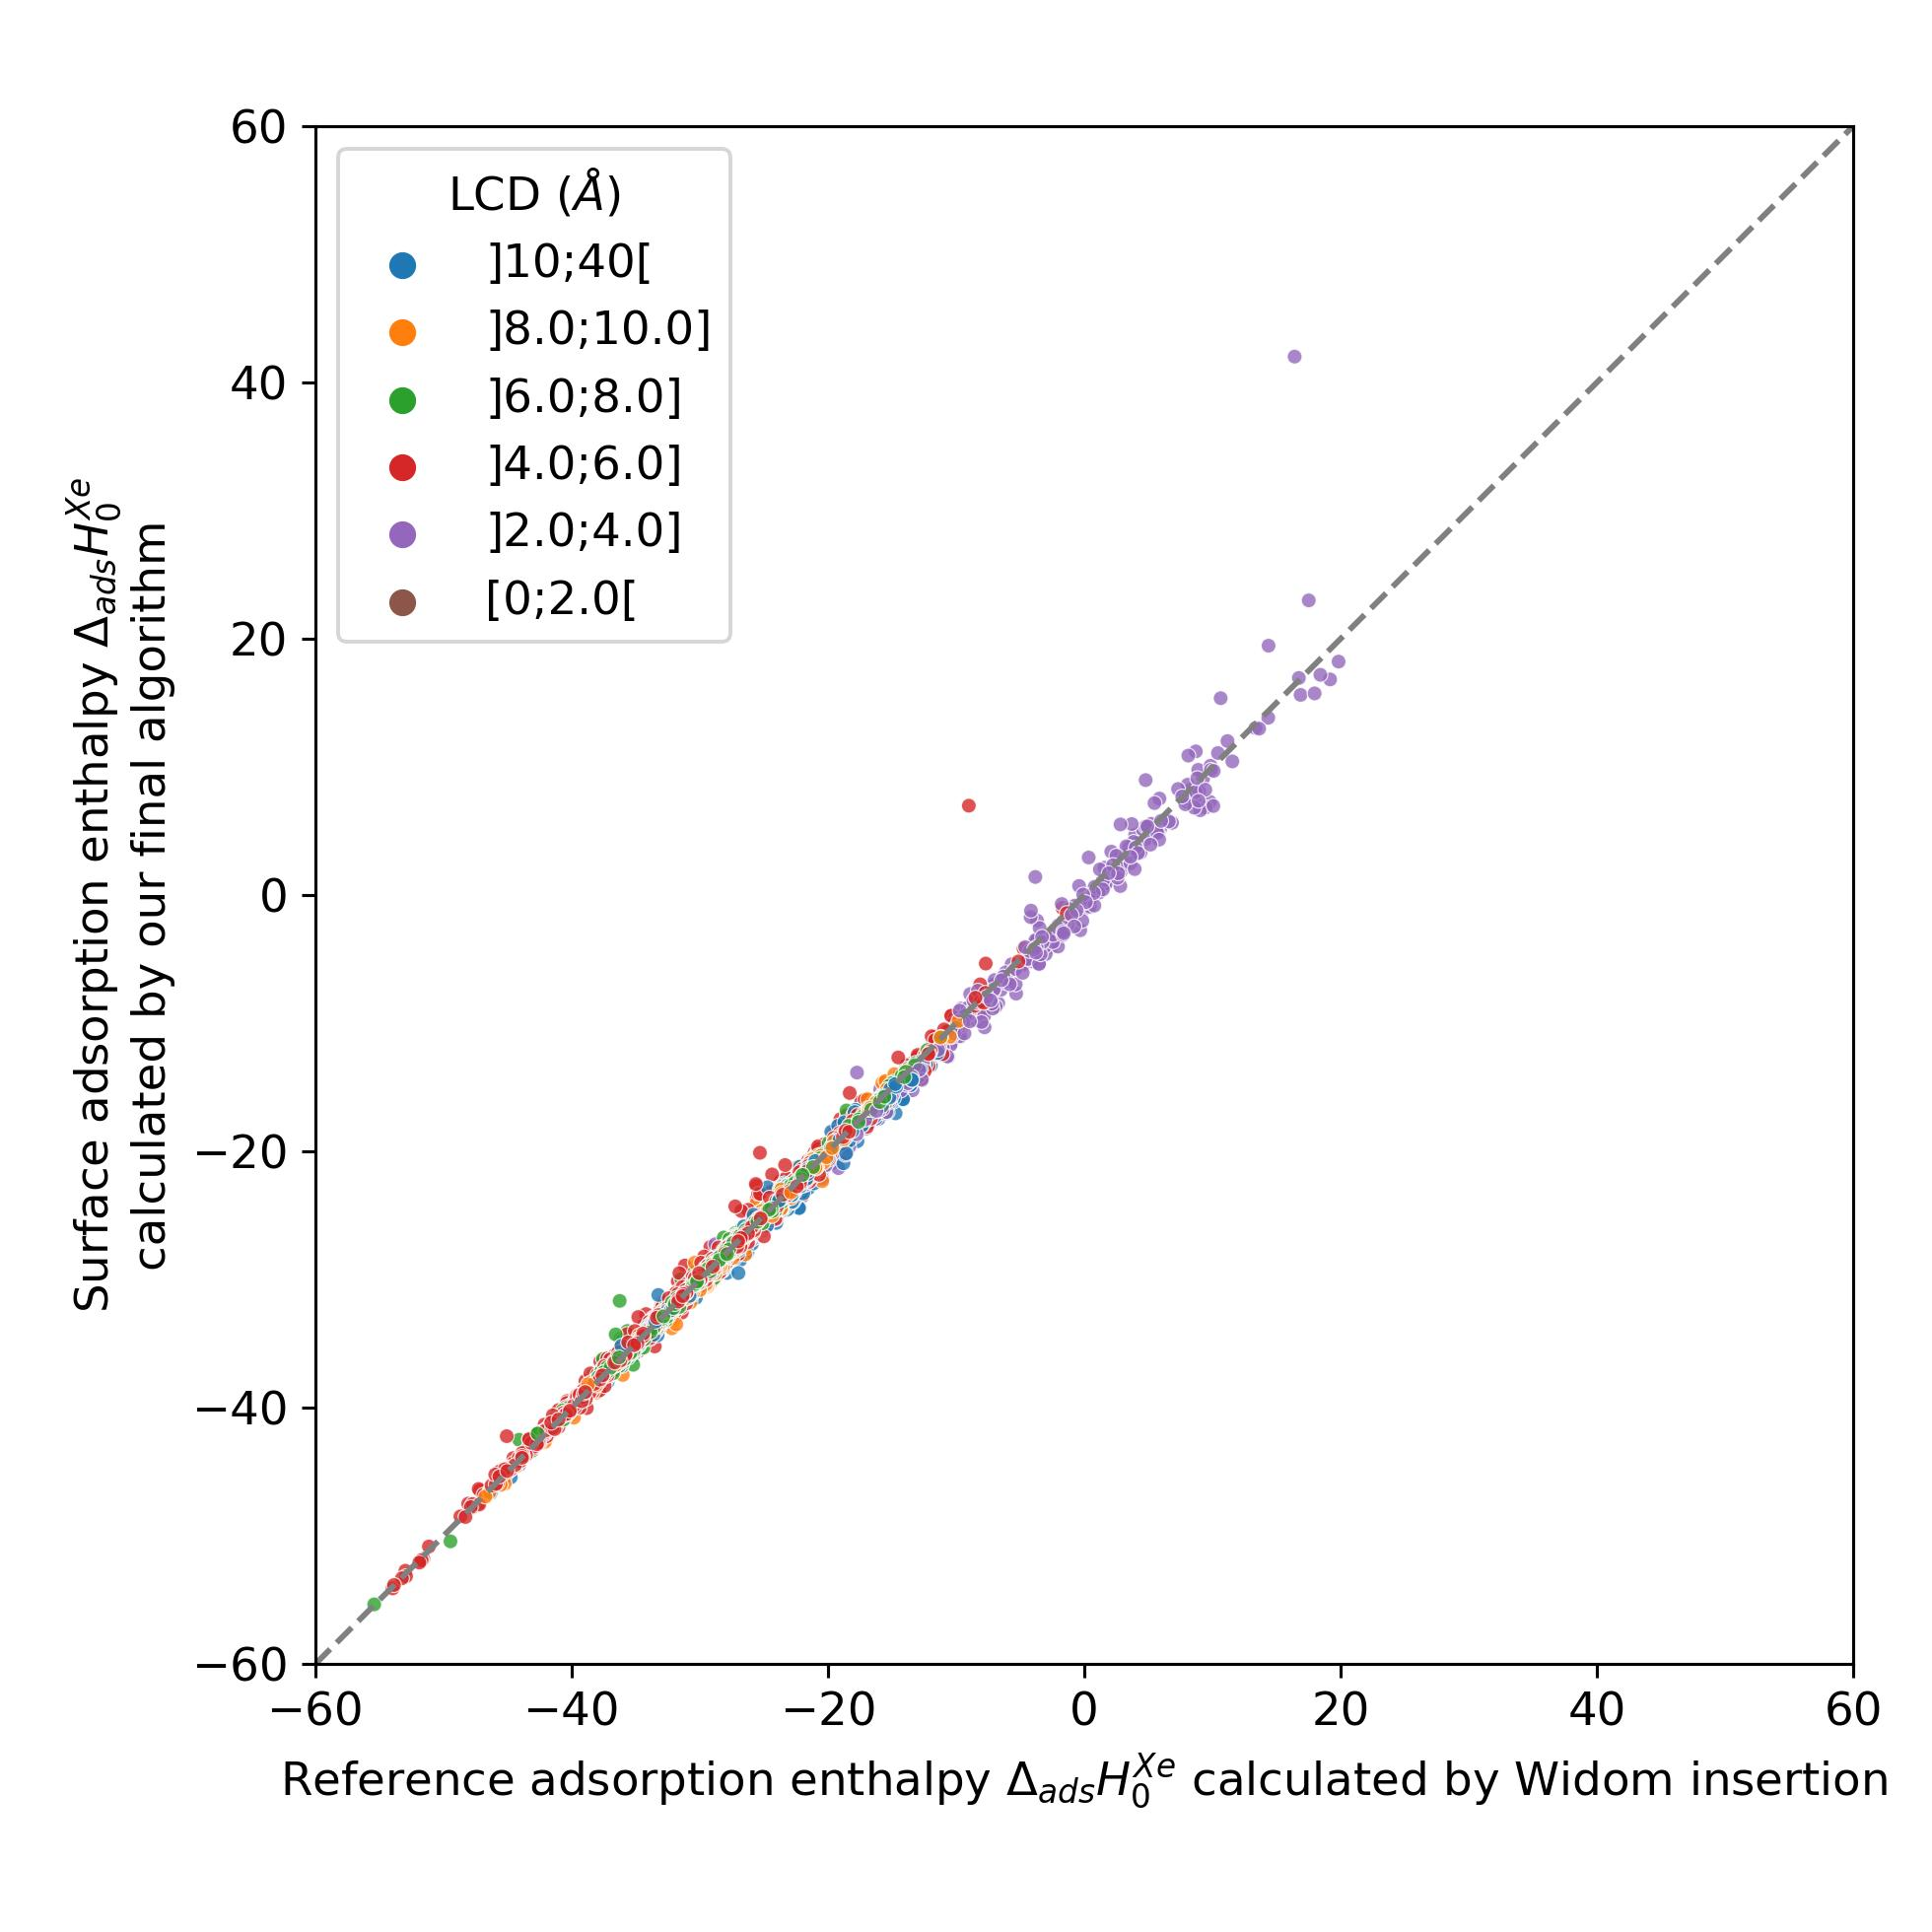
\includegraphics[width=0.45\linewidth]{figures/3-fastsim/H_Xe_widom_vs_H_Xe_surface_final_overview.jpg}
  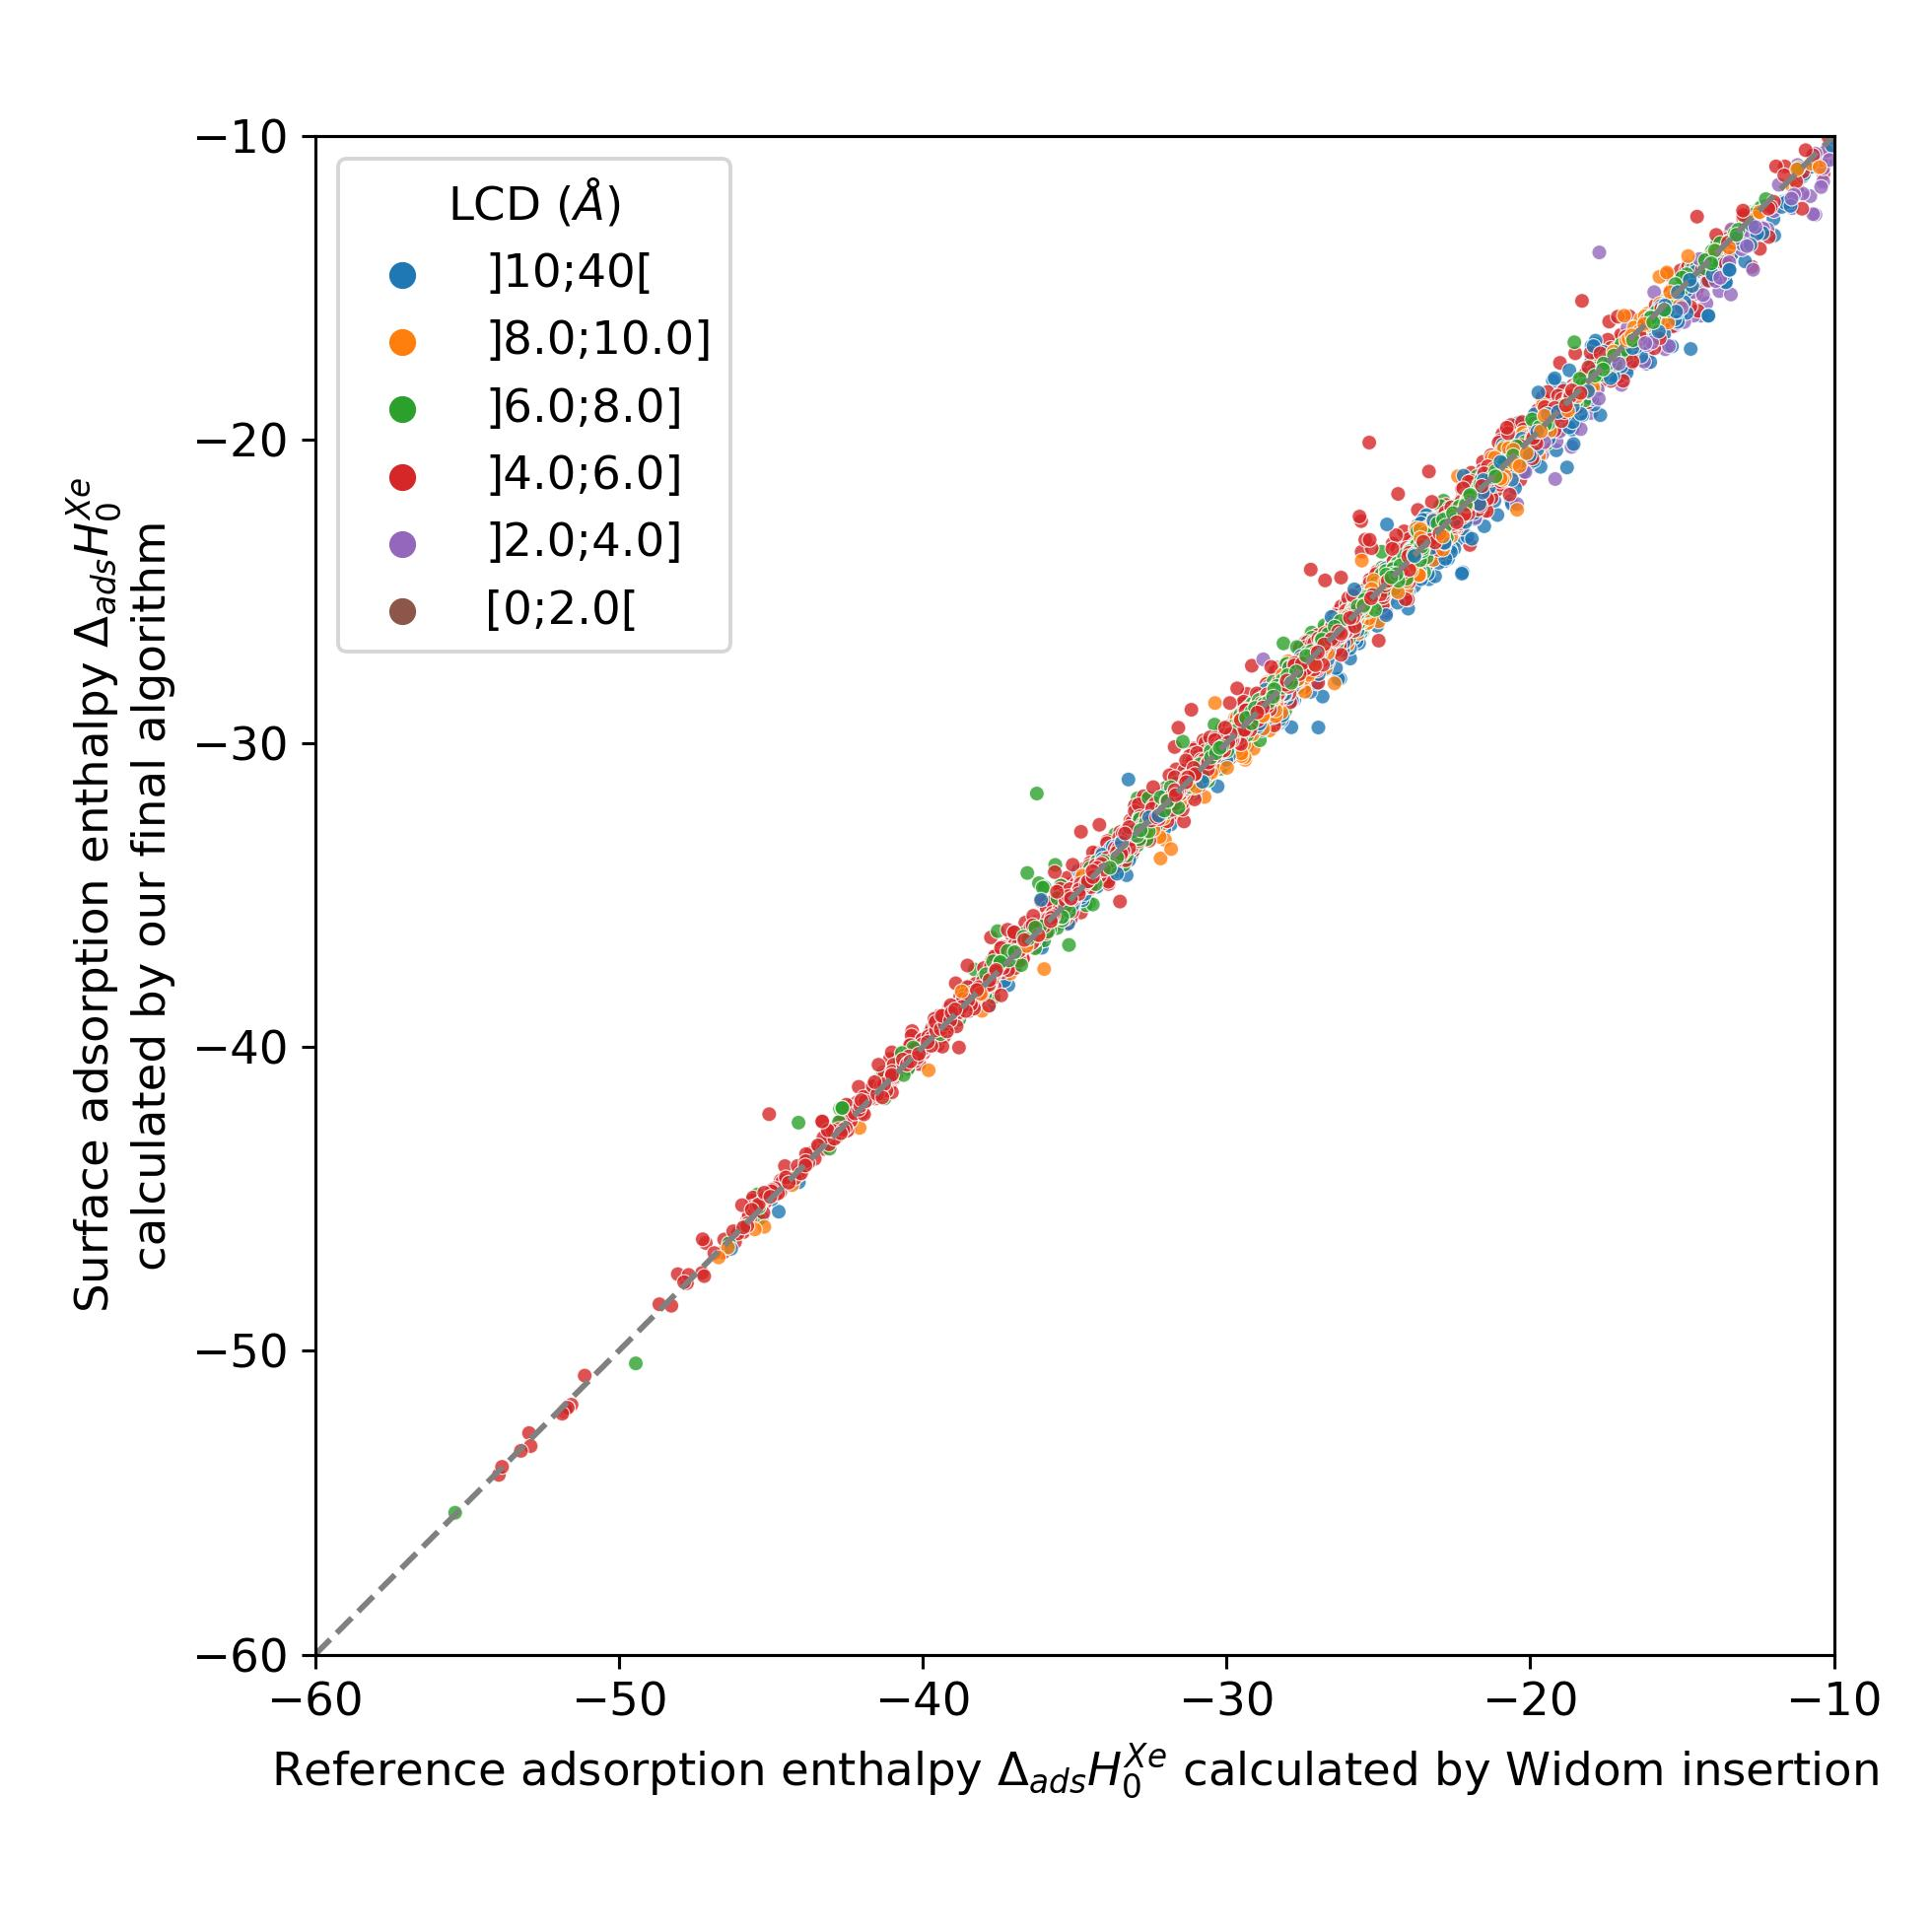
\includegraphics[width=0.45\linewidth]{figures/3-fastsim/H_Xe_widom_vs_H_Xe_surface_final_zoom.jpg}
    \caption{Scatterplots of the xenon surface adsorption enthalpy calculated by the final RAESS algorithm ($\lambda = 1.6$ and $\mu=0.85$) as a function of the xenon adsorption enthalpy calculated by a 100k-step Widom insertion simulation using two value windows, in structures of CoRE MOF 2019 with LCD\e{CCDC} $\geq$ \SI{3.7}{\angstrom} at \SI{298}{\kelvin}. The second plot zooms on the negative values corresponding to the most selective materials.}\label{fgr:surface_sampling}
\end{figure}

% \begin{table}[ht]
%   \centering
%   \begin{tabular}{|l|r|r|}
%   \hline
%                 Method &  RMSE (kJ/mol) &   Time (s) \\
%   \hline
%    surface\_standard\_2k &       0.903953 &   1.045269 \\
%      surface\_radius\_2k &       0.331715 &   1.145985 \\
%   surface\_rejection\_2k &       0.870635 &   0.234415 \\
%       surface\_final\_2k &       0.330454 &   0.339397 \\
%                voronoi &       2.114351 &   0.400000 \\
%              widom\_12k &       0.037631 & 145.058516 \\
%   \hline
%   \end{tabular}
%   \caption{Raw data of the performance of each sampling method}\label{tab:sumup}
% \end{table}

Finally, the values of the parameters optimized in this work might need adjustment when applied to other adsorption systems. The optimal $\mu$ parameter depends on the size of the adsorbent, and it should be tweaked differently when considering another adsorbent. For instance, the set of structures used for the optimization of $\mu$ depends on the size of their cavities, and the \SI{3.7}{\angstrom} threshold chosen here would need to be changed according to the kinetic diameter of the adsorbate. Furthermore, as aforementioned in the section on the rejection condition, it is possible to trade off a bit of accuracy for faster simulations especially in high-throughput screenings where speed is extremely important. Similarly, in the case of xenon, the cost of increasing the sphere size is around $10$ to {$20$\%}. On very large databases, one could consider that this increase on the required computational time is not worth the accuracy improvement, and one could decide to keep a smaller sampling sphere. If this method is transposed to different molecular systems, its parameters should be tested on the specific database and adsorbate of interest.

\begin{figure}[ht]
  \centering
    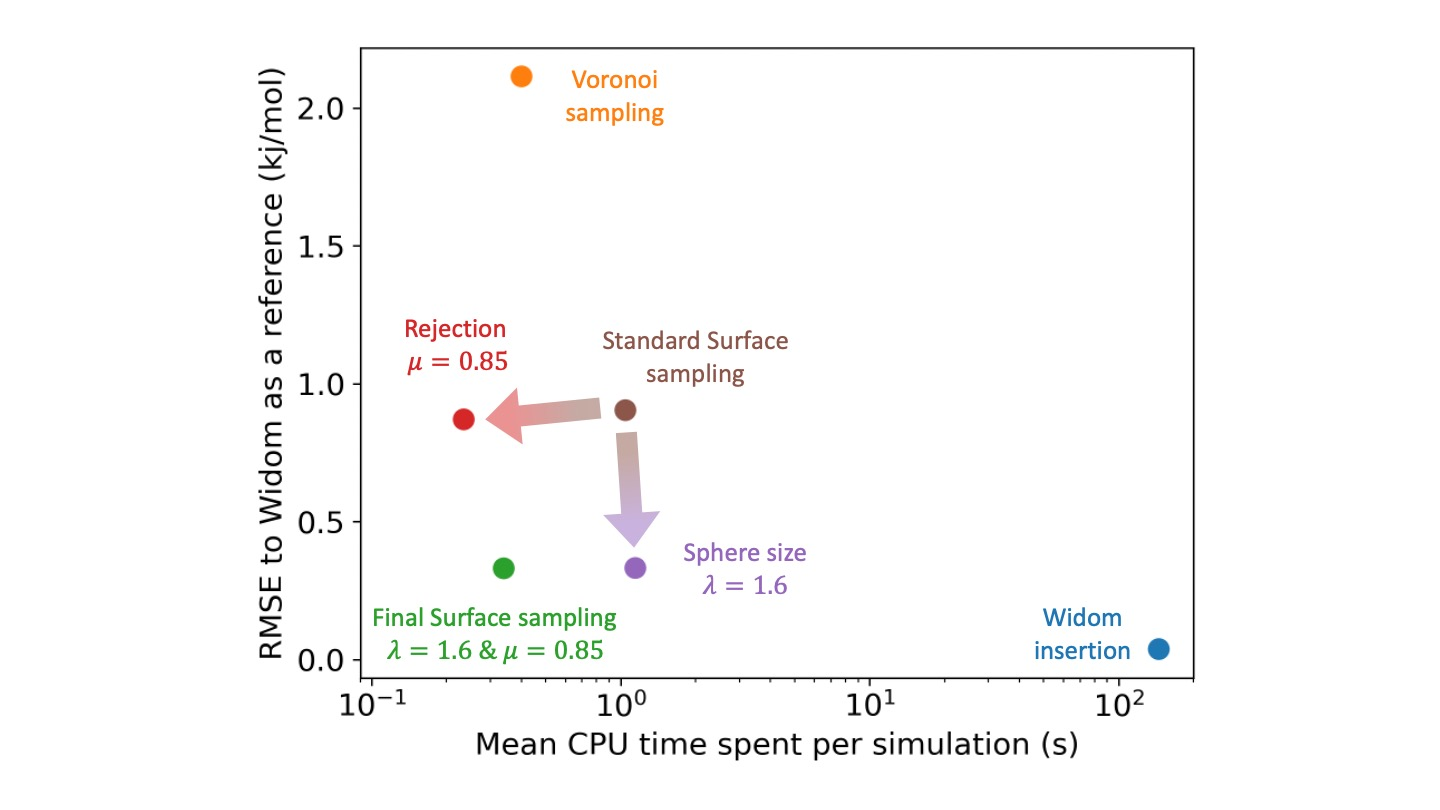
\includegraphics[width=\linewidth]{figures/3-fastsim/methods_comparison.jpg}
    \caption{Comparison of the RMSE to the reference Widom insertion and the average computation time for different types of enthalpy calculation methods. The surface sampling calculation was all done with 2k sampling points on each sphere and the Widom simulations were done using 12k cycles. These values correspond to the value at the convergence identified using Figure~\ref{fgr:convergence}. }\label{fgr:sumup}
  \end{figure}

\subsubsection{Calculation of Henry constant and surface area}

The main goal of the sampling algorithm is to calculate adsorption enthalpy in the zero-loading limit. The method can also calculate the Henry constant and surface area of the materials simultaneously, without incurring significant additional computational cost. The Henry constant serves as a key metric for assessing the affinity of an adsorbate to a nanoporous structure. The Xe/Kr gas selectivity at low pressure is defined as the ratio of the Henry constants of Xe and Kr. This important property can be determined using Equation~\ref{eq:eq_cst} in a Widom insertion calculation. Instead of utilizing the interaction energies at the Widom inserted points, an approximate value for the Henry constant can now be obtained using the surface sampled points.

\begin{figure}[ht]
  \centering
  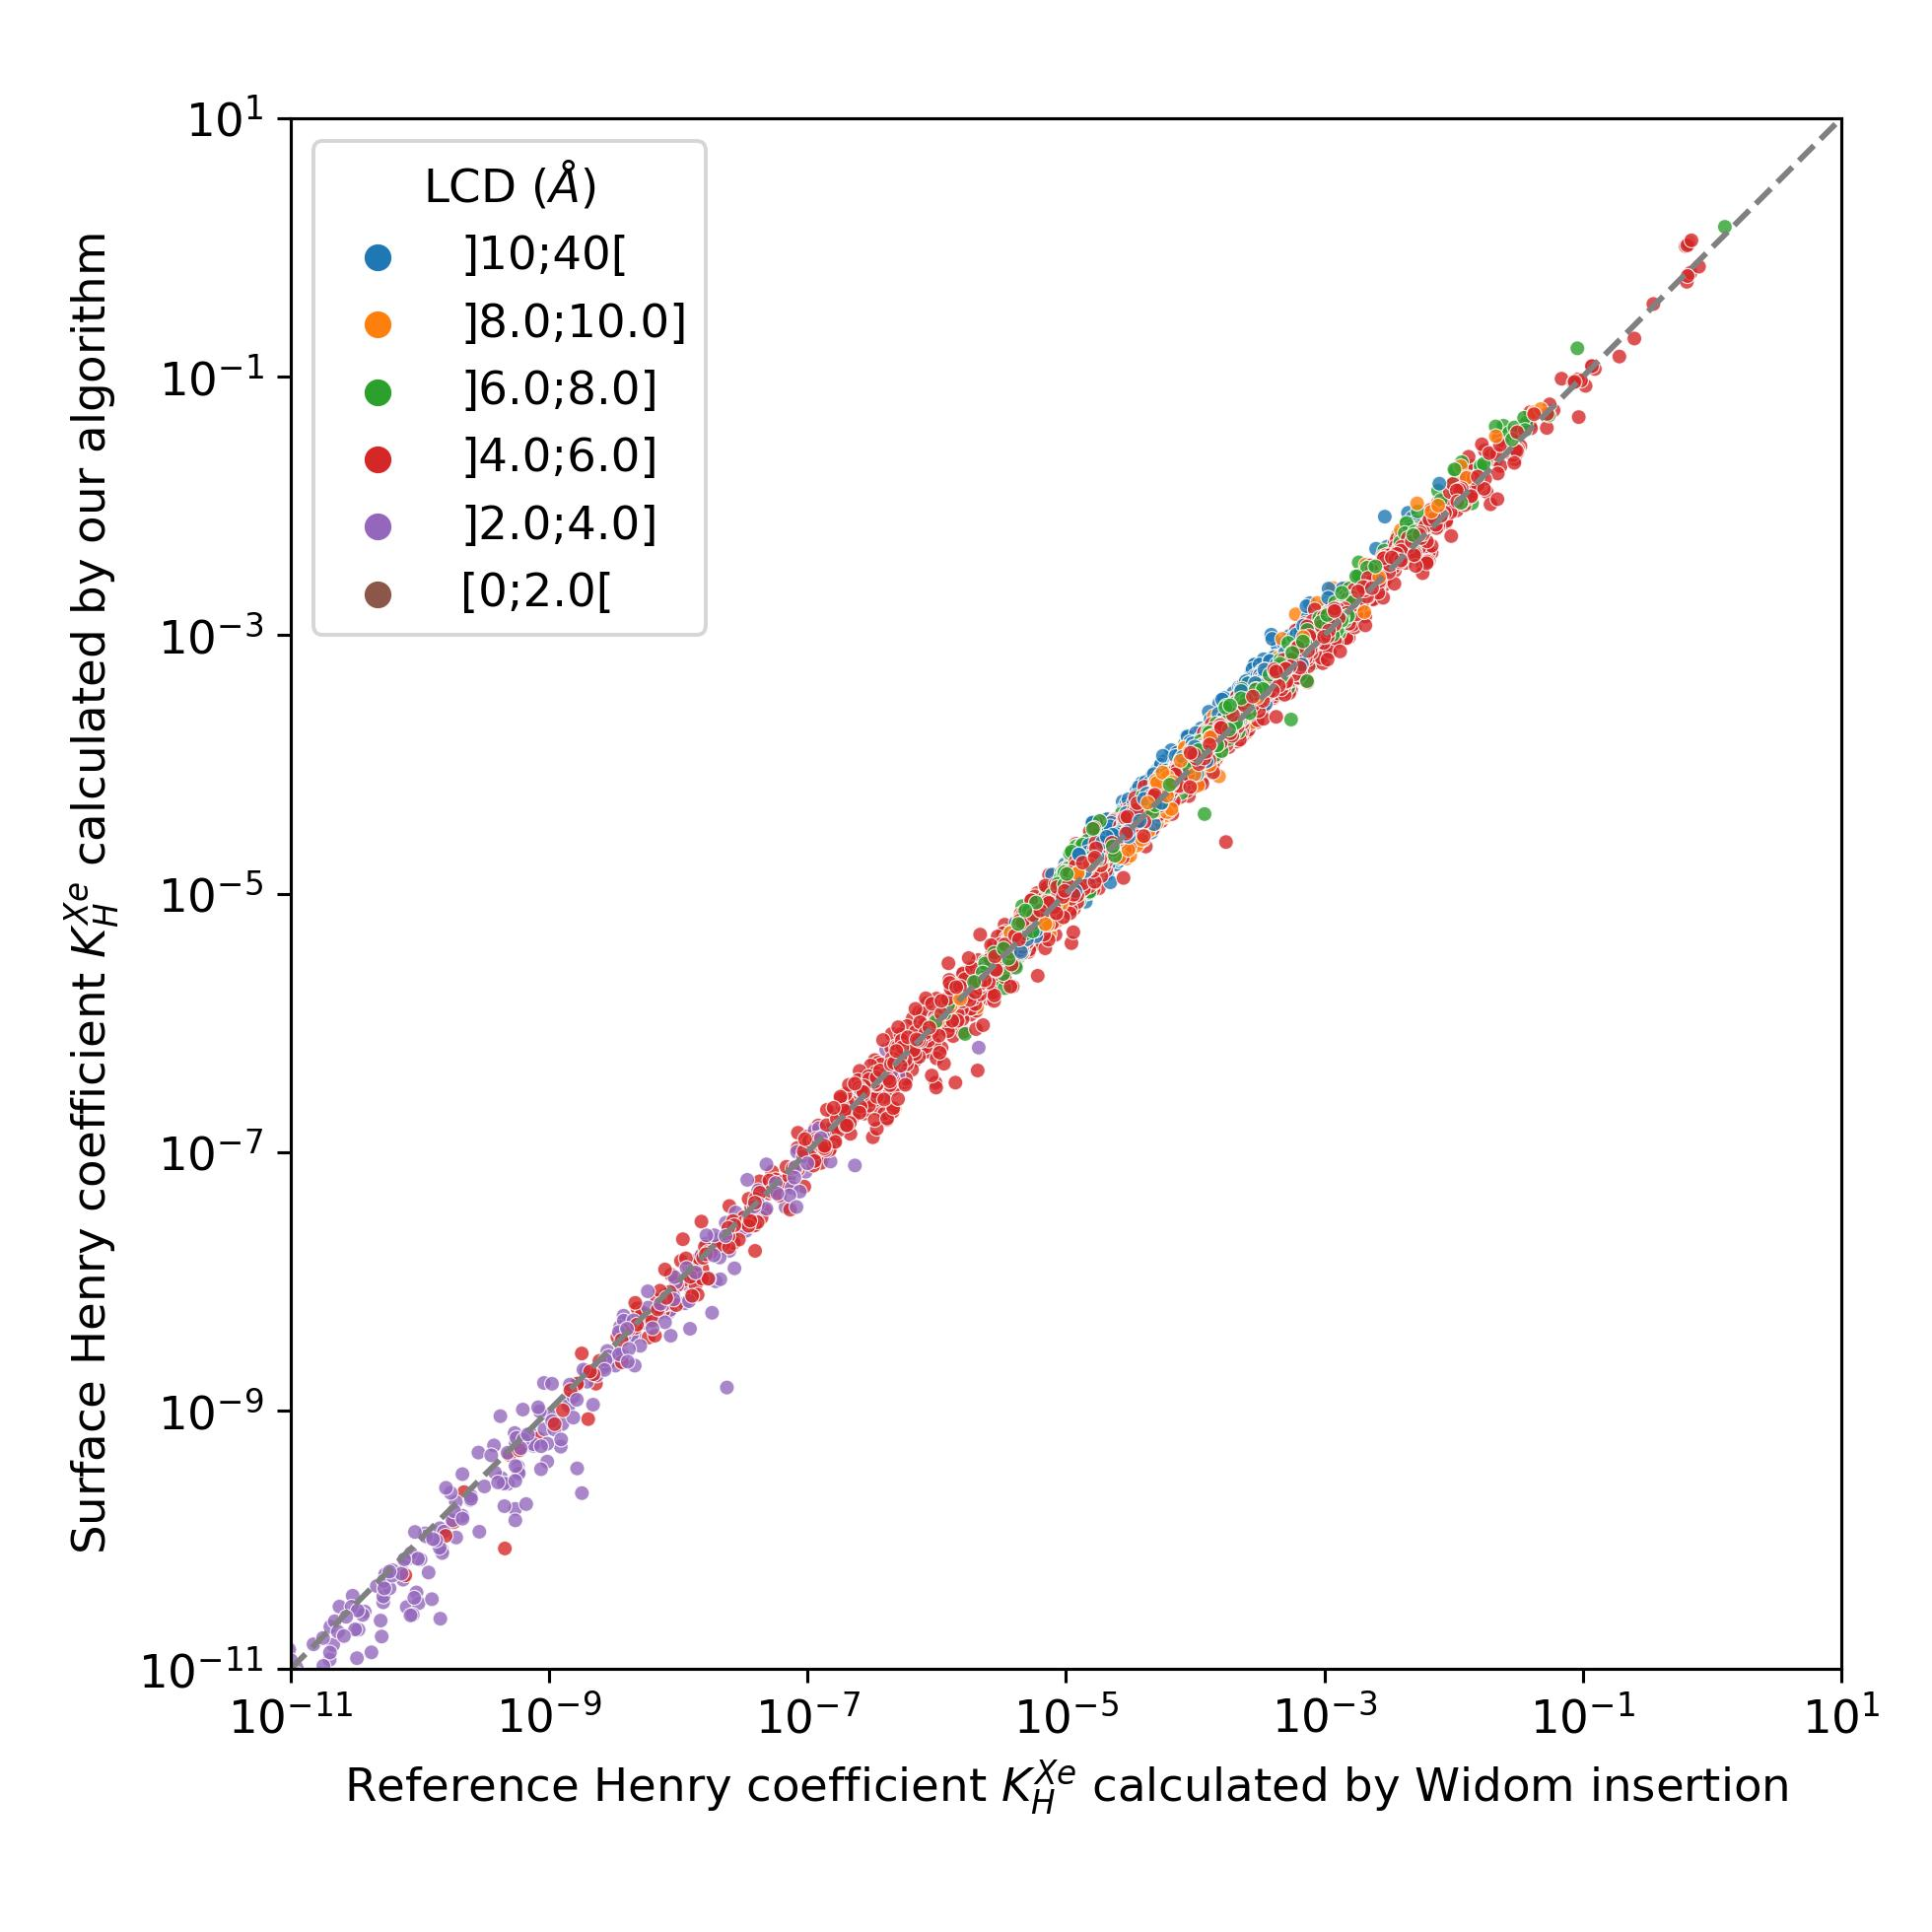
\includegraphics[width=0.6\linewidth]{figures/3-fastsim/K_Xe_widom_vs_K_Xe_surface_final_zoom.jpg}
    \caption{Scatterplots of the xenon Henry constants calculated by the RAESS algorithm compared to the ones calculated by a 100k-step Widom insertion simulation using two value windows.}\label{fgr:henry_scatter}
\end{figure}

By employing the optimized set of parameters for surface sampling, the algorithm's performance in estimating the Henry constant was assessed by comparing it to the ground truth obtained through 100,000 cycles of Widom insertion. Since the Henry constant corresponds to the exponential of an adsorption free energy and the focus of this study lies on the precision of the free energy, a log-scale evaluation metric is used. For surface sampling, the log-RMSE of $K\e{H}$ is equal to $0.2$, indicating that the values are accurately predicted in terms of order of magnitude, as depicted in Figure~\ref{fgr:convergence_free_energy}. If the derived free energy $\Delta F_{ads} = -RT \log(\rho_fRT K_H)$ is considered, the RMSE is approximately \SI{1.1}{\kilo\joule\per\mole}, and this level of error is achieved within a similar amount time of approximately \SI{1}{\second} (Figure~\ref{fgr:convergence_free_energy}). In contrast, for Widom insertion, a similar level of error is attained within a similar time frame, and an RMSE of approximately \SI{0.1}{\kilo\joule\per\mole} is achieved within \SI{86}{\second} (Figure~\ref{fgr:convergence_free_energy}). For free energy calculation, surface sampling converges 86 times faster. If the main focus is on adsorption enthalpy, the Henry constant can be computed with minimal additional computational cost and reasonable accuracy, thereby obtaining two thermodynamic properties of interest for the cost of one.

\begin{figure}[ht]
  \centering
  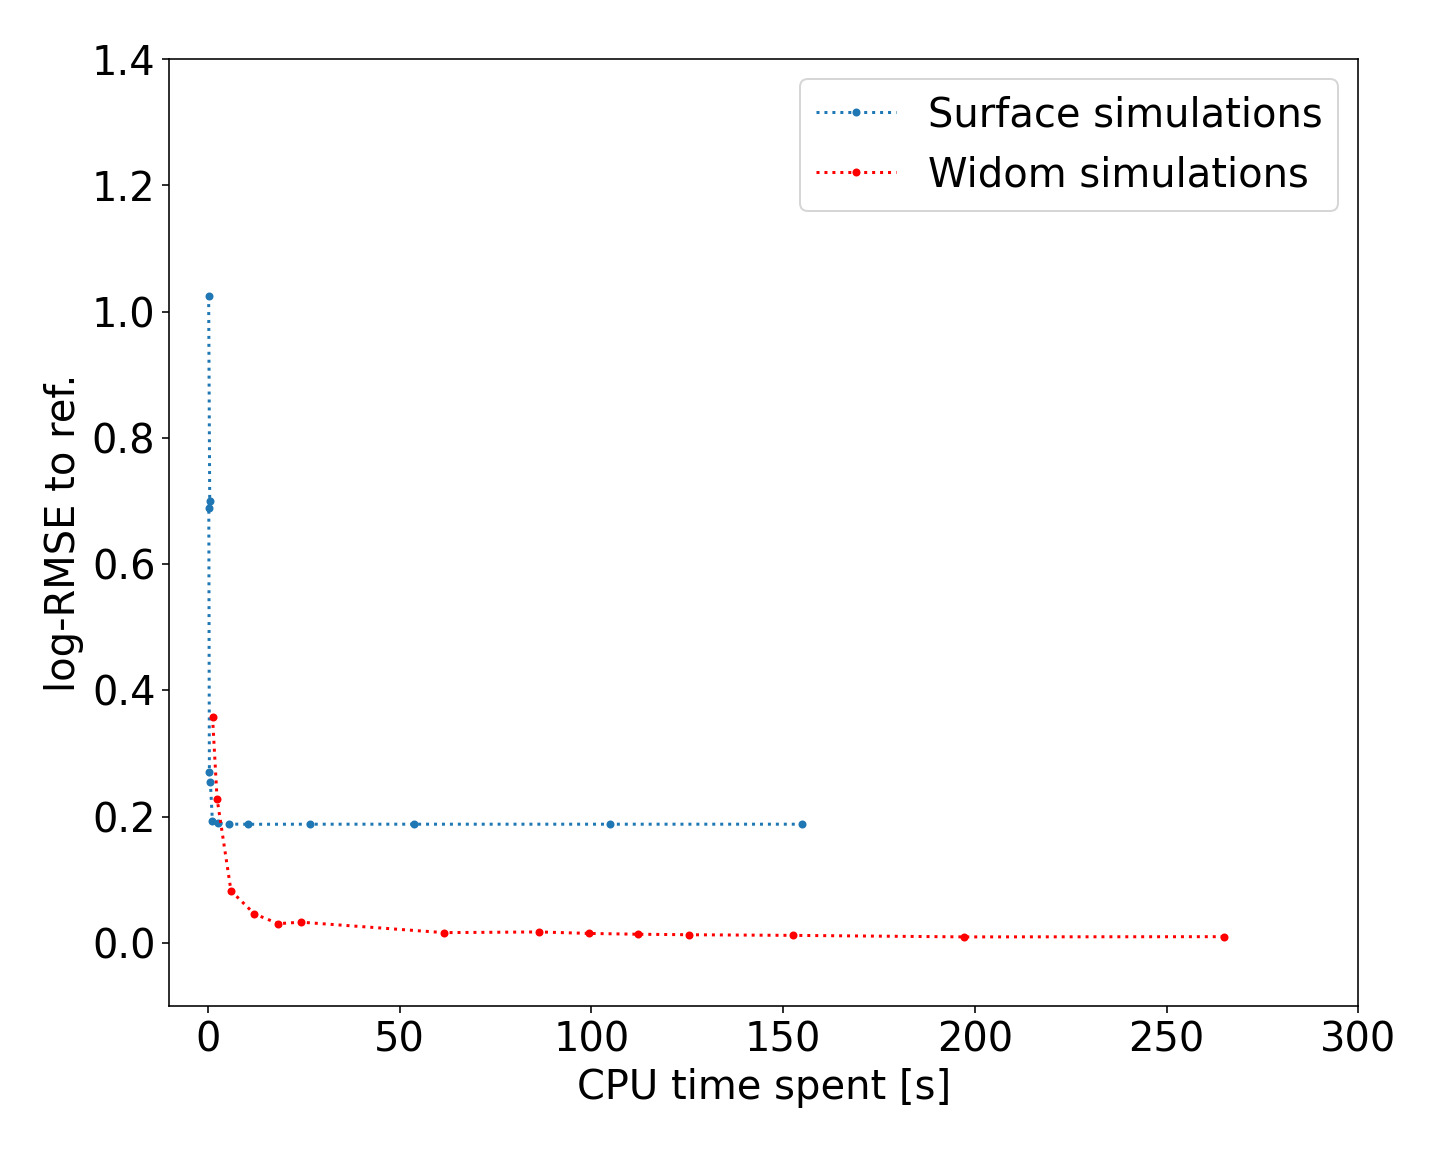
\includegraphics[width=0.45\textwidth]{figures/3-fastsim/log_henry_convergence.jpg}
  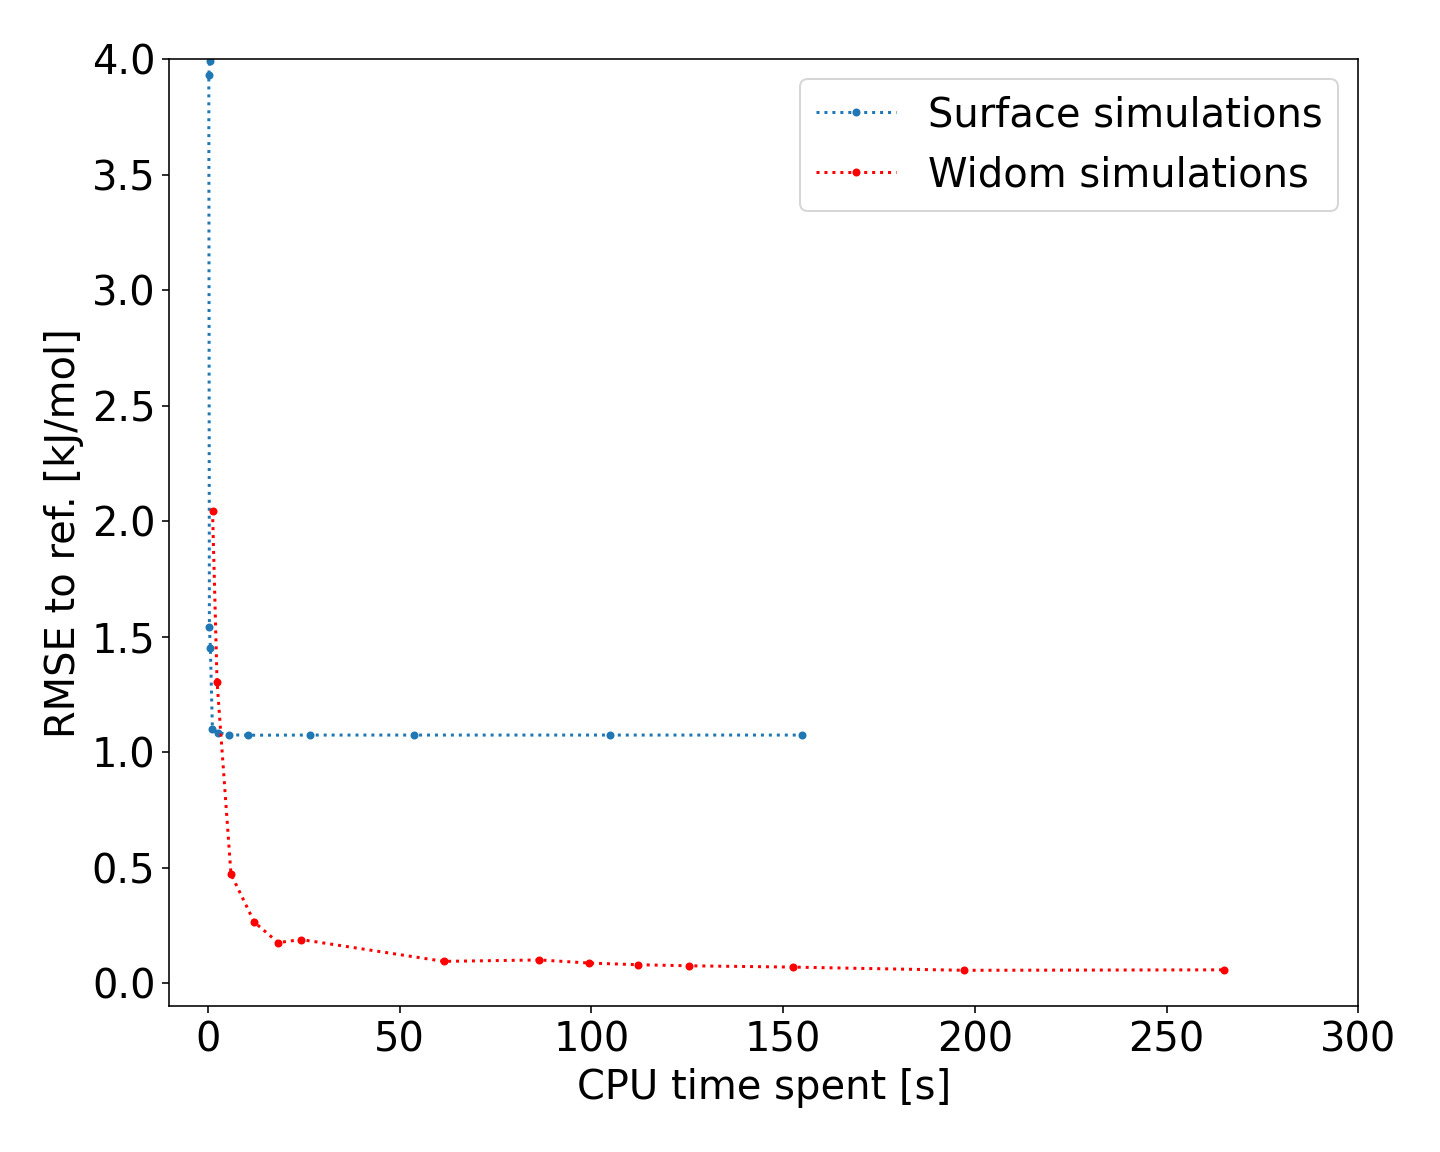
\includegraphics[width=0.45\textwidth]{figures/3-fastsim/gibbs_free_energy_convergence.jpg}
  \caption{ Left: convergence plot of the log-RMSE on the xenon Henry constants for both the surface sampling and the Widom insertion. Right: convergence plot of the RMSE on the xenon adsorption Gibbs free energy for the final implementation of the surface sampling and the Widom insertion. }\label{fgr:convergence_free_energy}
\end{figure}

Similarly, the algorithm can be adapted to determine the surface area of the material by counting the number of points within the sampling spheres that possess negative energy and represent the points where guest moleculess can interact favourably. By dividing this count by the total number of sampled points, the proportion of adsorbable area is obtained for each sphere. Summing these proportions over all atoms yields the total surface area. This implementation is summarized in equation~\ref{eq:sa}:
\begin{equation}
\label{eq:sa}
    \textrm{SA} = \dfrac{1}{V}\sum_{a\in \textrm{cell}} \dfrac{N\e{accessible}(a)}{N\e{total}}4\pi {r(a)}^2
\end{equation}
where $V$ volume of the cell $a$ atoms of the cell; $N_{accessible}(a)$ accessible points around the atom $a$; $N_{total}$ sampling points; $r(a)$ radius of the sampling sphere around the atom $a$.
When $\lambda=1$, spheres with a radius $\sigma$ are sampled, which is equivalent to considering hard spheres defined by $\sigma$ (a convention used by RASPA2 to calculate surface areas). When comparing simulations with $\lambda=1$ to those obtained by RASPA2, the surface areas are found to be very close (see Figure~\ref{fgr:surface_area} in SI). However, when considering $\lambda=1.6$, the previously observed perfect agreement is lost, and the points show weak correlation in log-scale (see Figure~\ref{fgr:surface_area} in SI). This difference can be attributed to the larger sphere size, which also alters the proportion of adsorbable points. The relationship between these two adsorption surface areas is far from trivial. Due to the relatively low computational cost of surface area calculation, this implementation would not be highly useful, except for obtaining a rough estimate of the surface area.

\begin{figure}[ht]
  \centering
  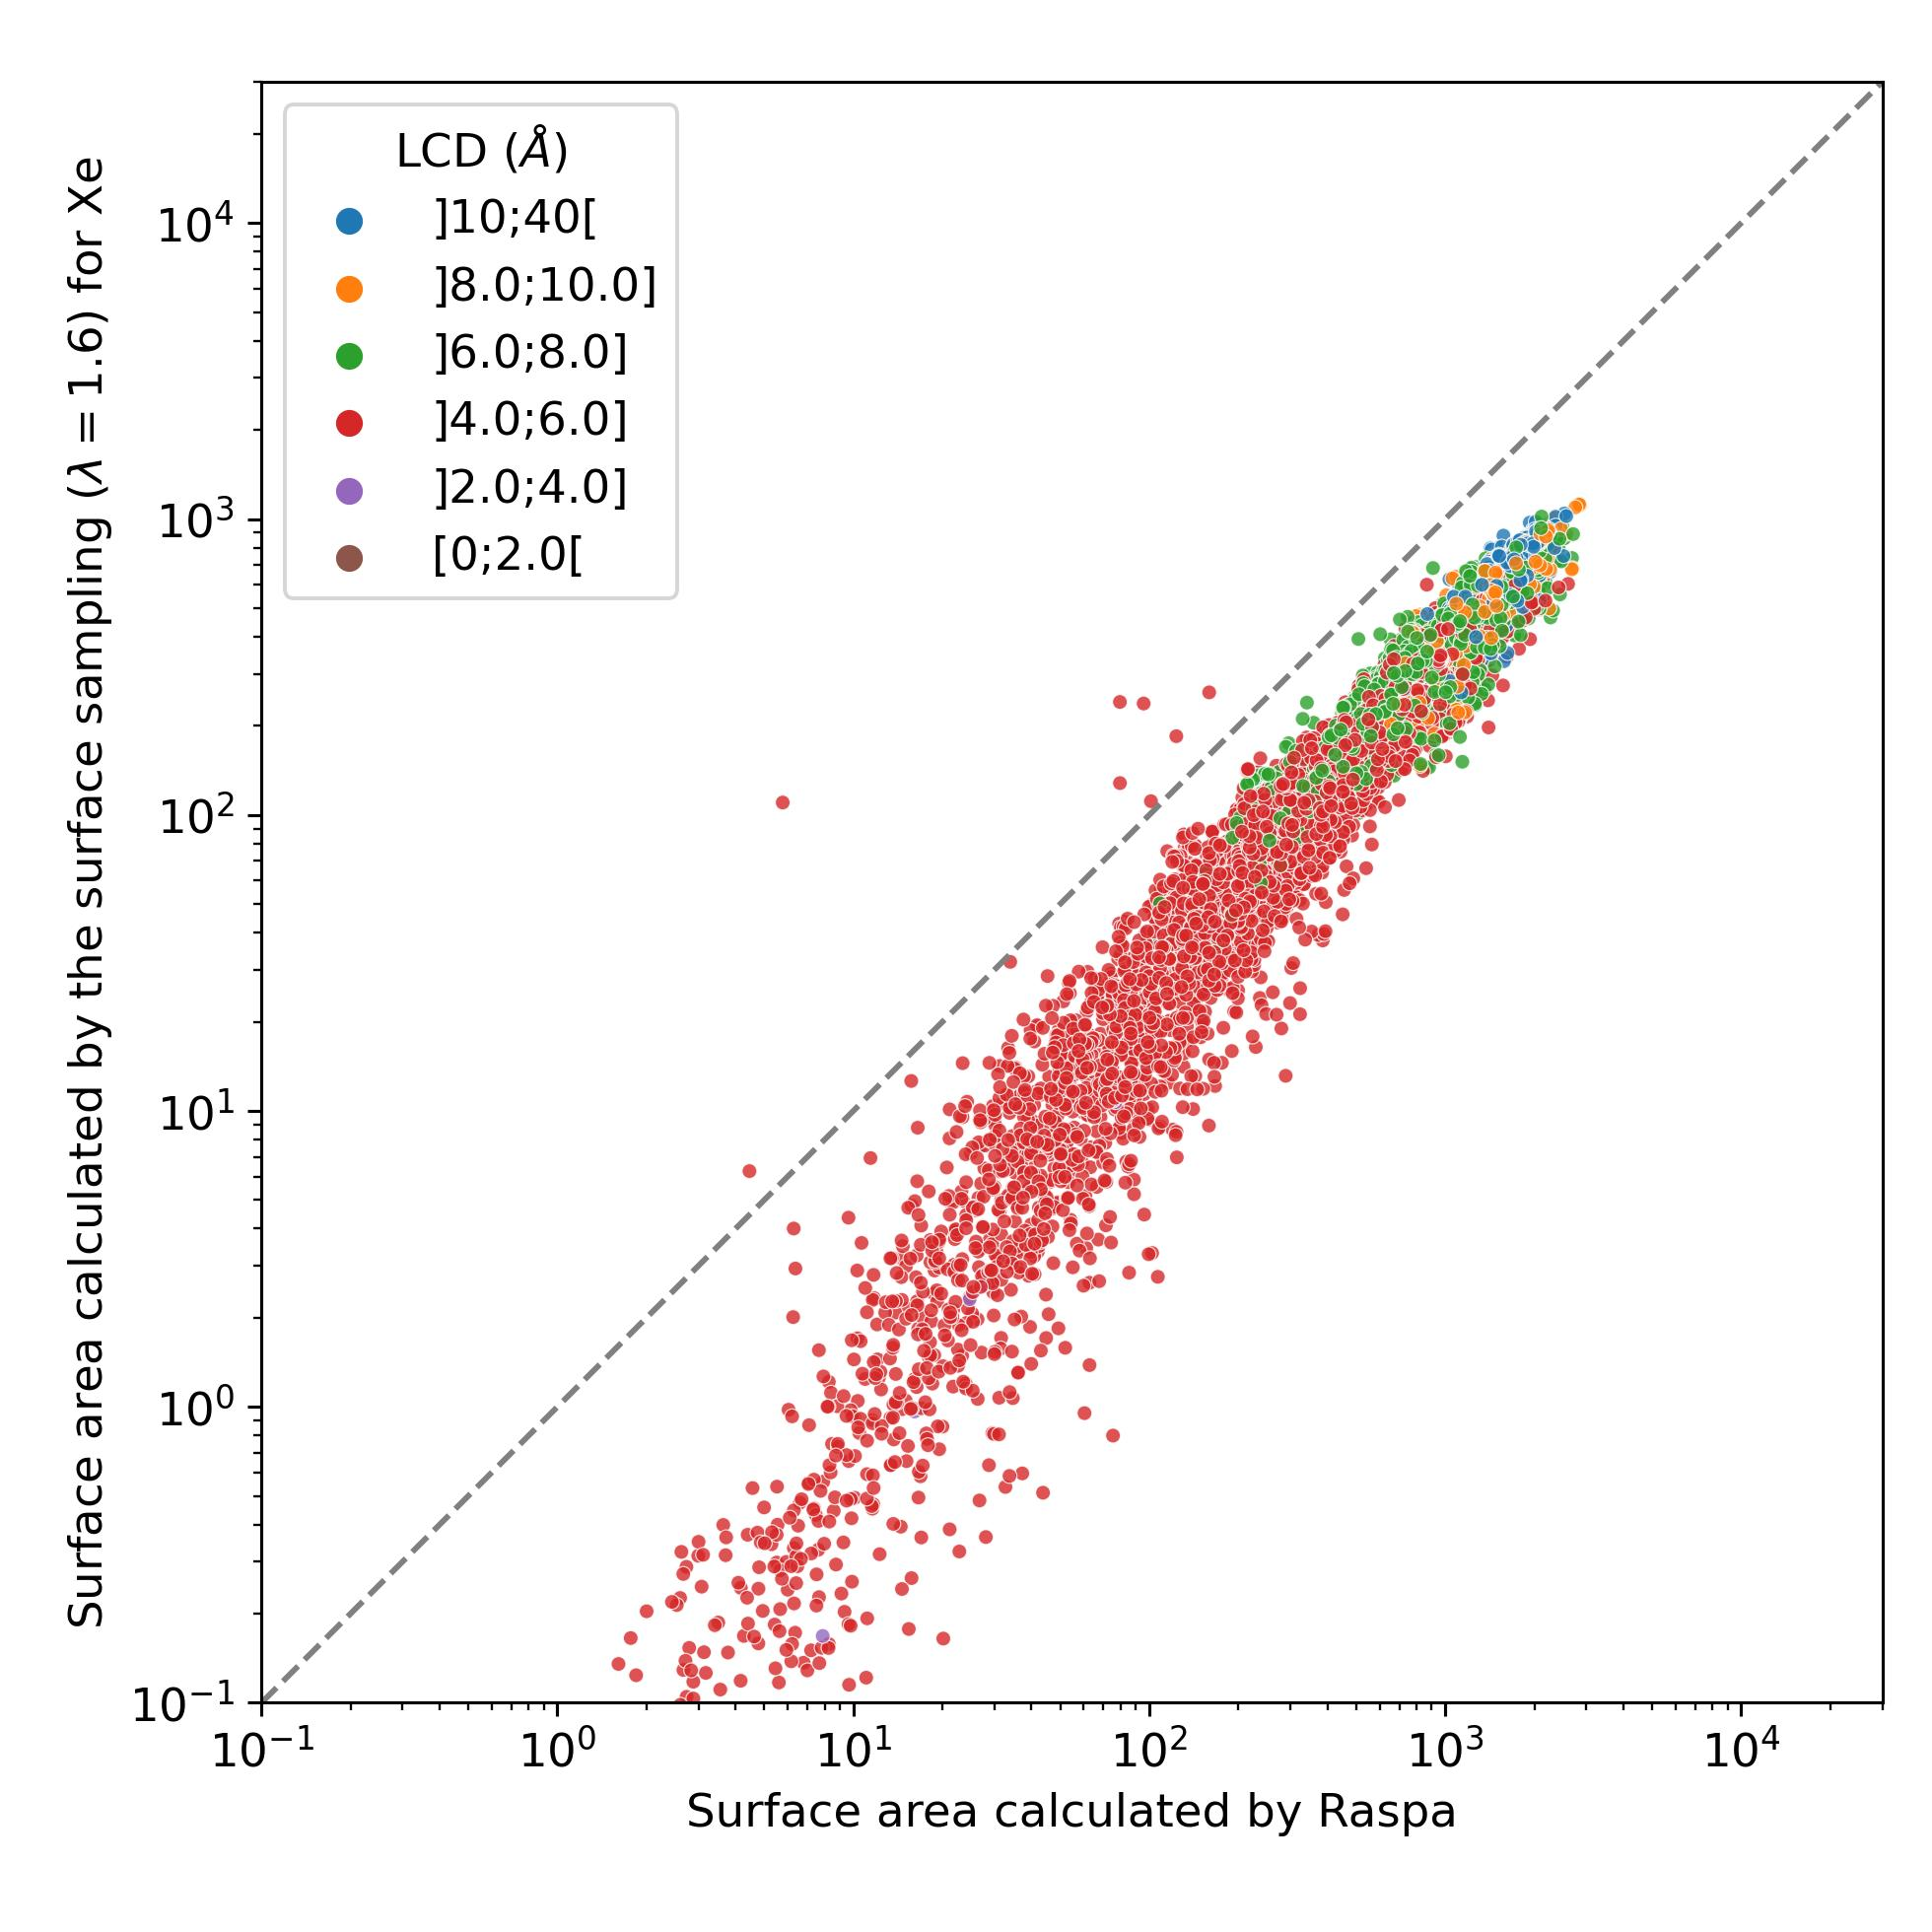
\includegraphics[width=0.45\textwidth]{figures/3-fastsim/SA_raspa_Xe_m3_cm3_vs_SA_lambda_1.6_overview.jpg}
  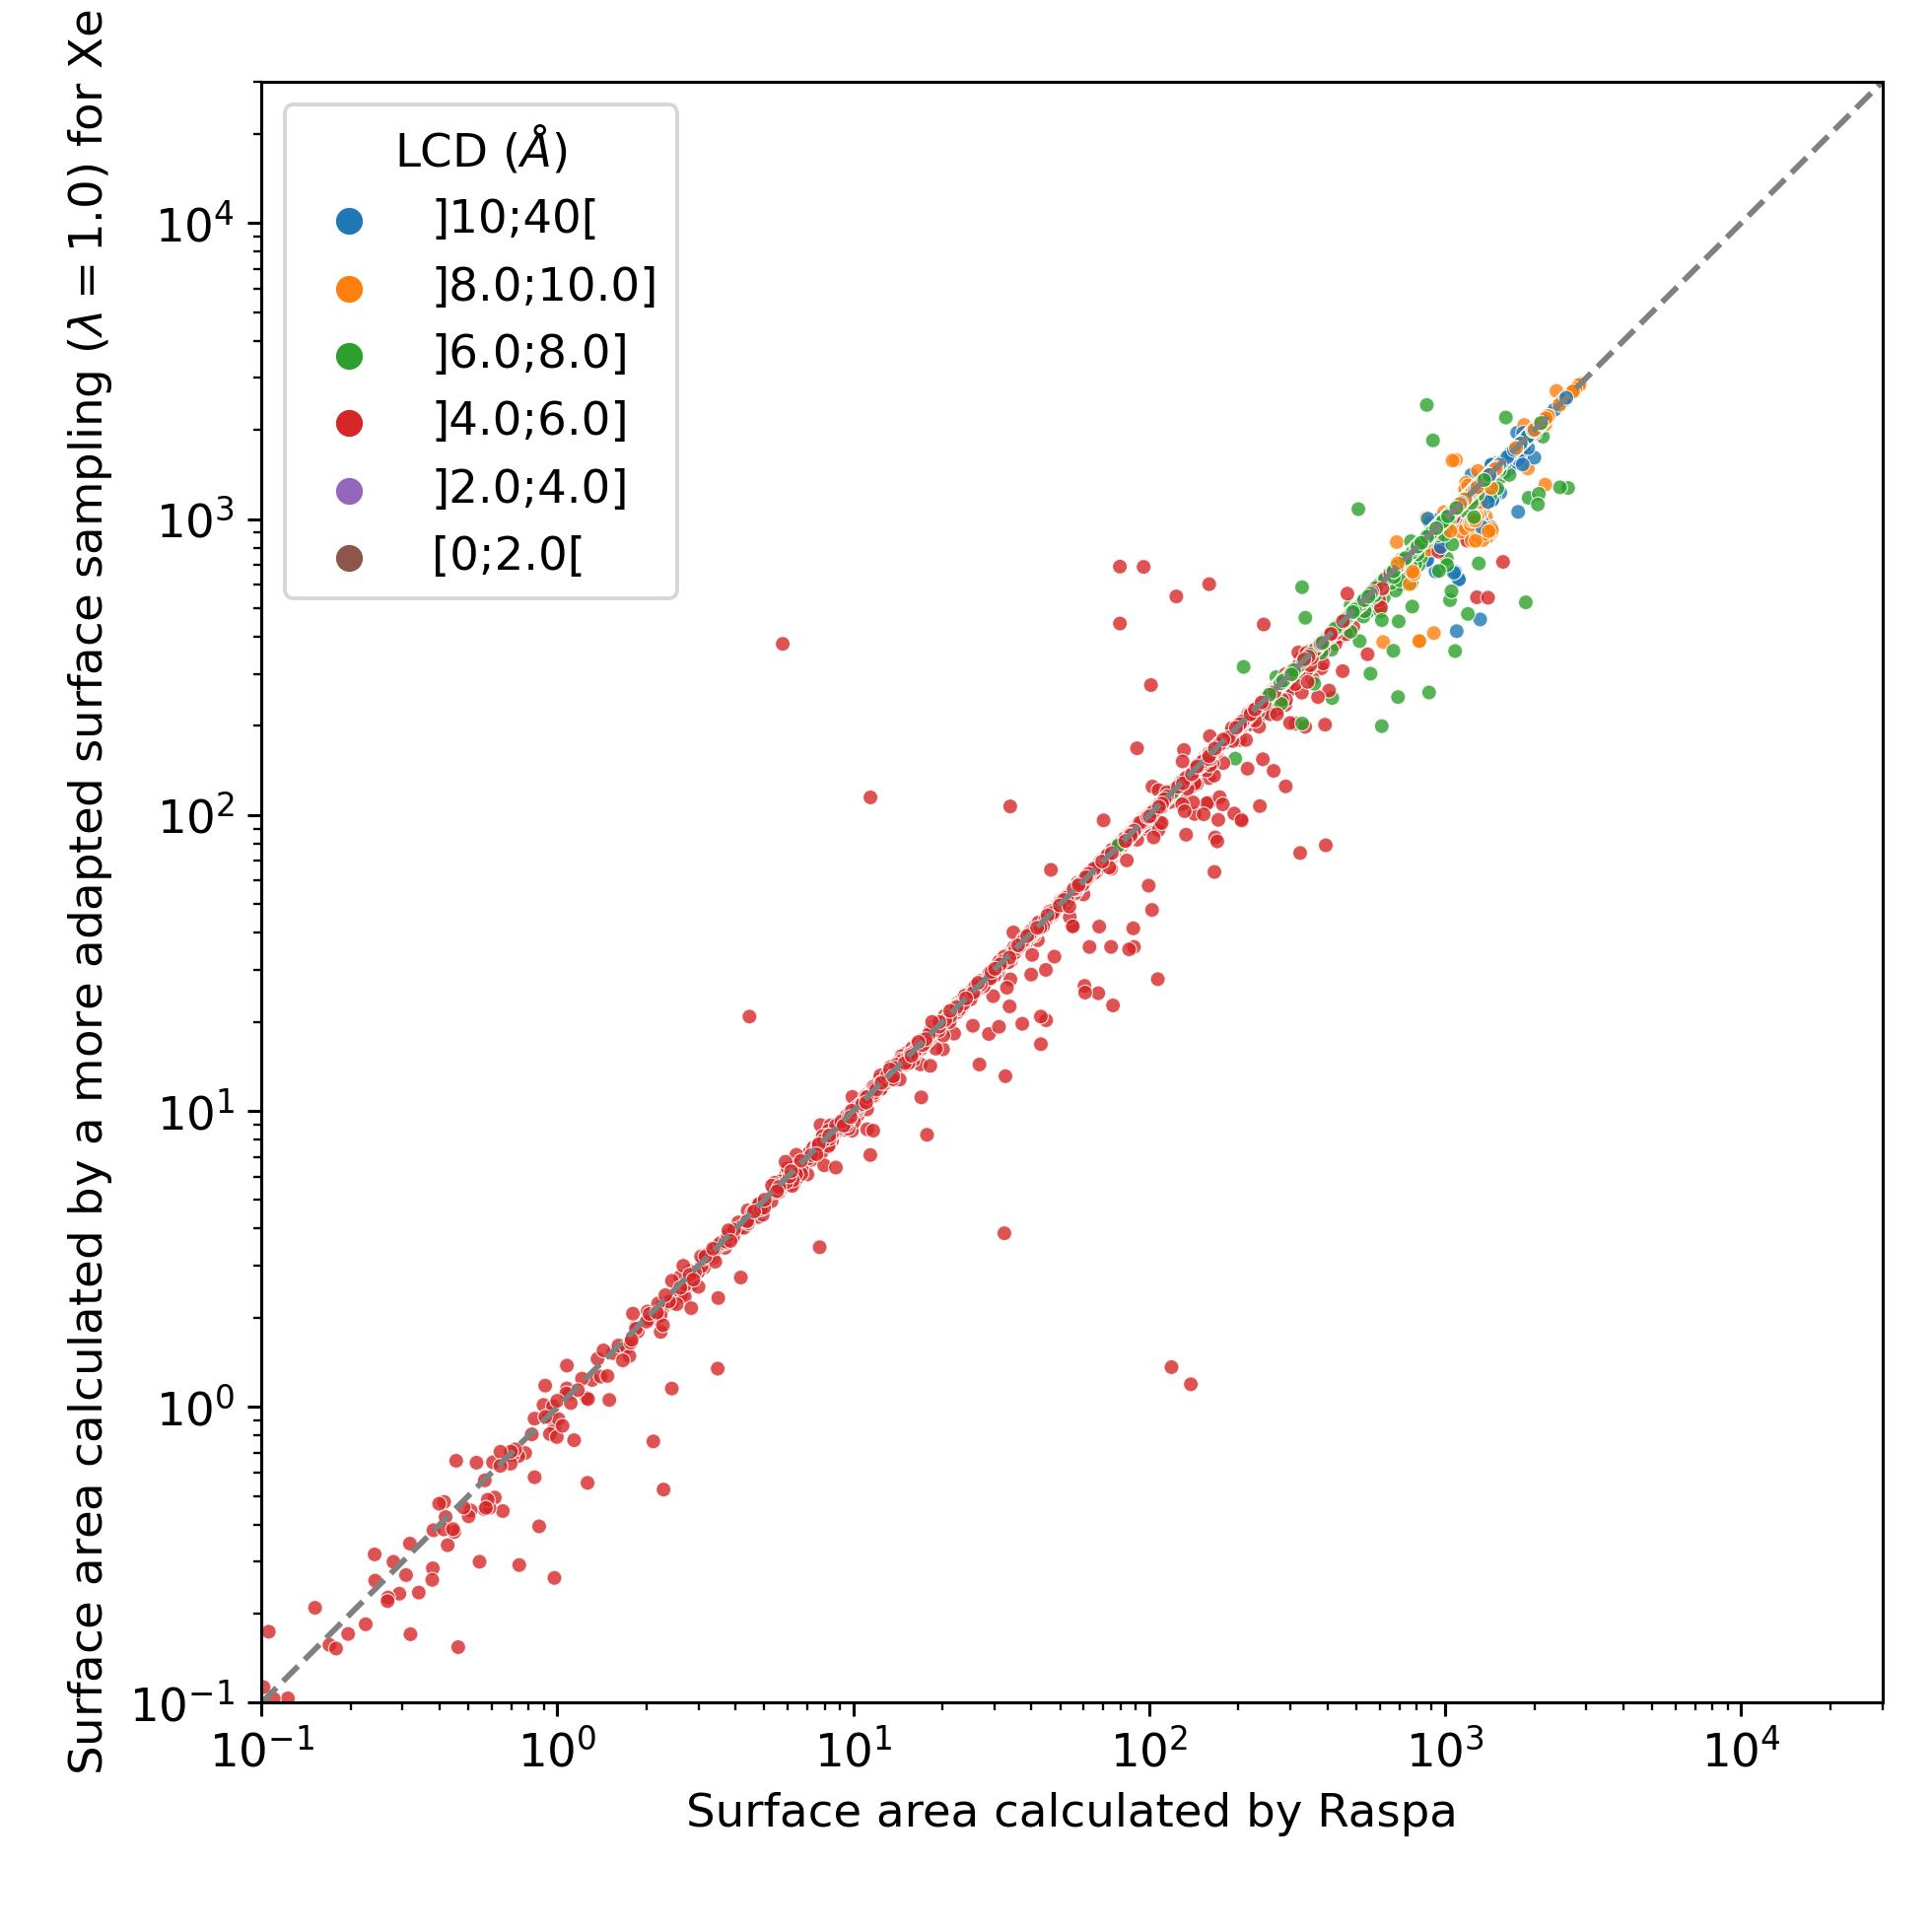
\includegraphics[width=0.45\textwidth]{figures/3-fastsim/SA_raspa_Xe_m3_cm3_vs_SA_lambda_1.0_overview.jpg}
  \caption{Scatterplots of the surface areas calculated by the RAESS algorithm with two different parameterizations compared to the surface area given by a RASPA2 surface area calculation. The left plot corresponds to the surface sampling described in the section~\ref{sct:final_sampling} with $\lambda=1.6$ and $\mu=0.85$, while the right plot uses a sampling sphere near $\sigma$ with $\lambda=1.0$. The second parameterization is much closer to what a RASPA2 sampling based on the $\sigma$ parameter of a LJ potential does, hence explaining the much better agreement. }\label{fgr:surface_area}
\end{figure}

\subsection{Surface sampling application use cases}

After introducing the performance of the surface energy sampling algorithm for xenon and specific materials from CoRE MOF 2019 at \SI{298}{\kelvin}, further investigations on other conditions will be conducted to test the transferability of the methodology. First, the algorithm will be used to assess the xenon/krypton selectivity at infinite dilution, in comparison to the standard Widom insertion. Secondly, the influence of temperature on the algorithm's performance will be compared, as the performance may be less optimal due to the less concentrated Boltzmann weights on the less attractive points. Lastly, the RAESS algorithm will be tested on databases containing diverse materials.

\subsubsection{Selectivity Calculations}

The selectivity value, which is the most important metric in evaluating the Xe/Kr separation performance of a nanoporous material, is examined in this study to assess whether a surface sampling technique can accurately evaluate this metric while being limited by all the approximations inherent to the technique. 

A few precautions should be considered before blindly using the algorithm for selectivity prediction. During the investigation of selectivity calculation, it was observed that the rejection condition on xenon can be high, as the focus if this study is on identifying the most favorable materials for xenon adsorption. However, for krypton, it is necessary to accurately describe very low Henry constants, as a selective material would also exhibit unfavorable characteristics for krypton. Therefore, the parameter $\mu$ needs to be chosen wisely, ensuring that it is low enough to obtain accurate Kr Henry constant and selectivity values. 

As shown in Table~\ref{tab:selec_prob}, the error in selectivity highly depends on the $\mu$ value, which determines the exclusion of points at $\mu\sigma$ from a framework atom center. Intuitively, a lower $\mu$ enables the sampling of higher energy values that contribute to the Boltzmann averaging. Additionally, dividing by smaller values can amplify any errors in the values, and this effect can be mitigated by increasing the number of sampled points.

\begin{table}[ht]
  \setlength{\extrarowheight}{1pt}
  \centering
  \begin{tabular}{|l|r|r|}
  \hline
    rejection parameter $\mu$ &  log10-RMSE to 100k-Widom &   log10-MAE to 100k-step Widom \\
  \hline
      0.85 &      0.107 &   0.077 \\
      \textcolor{red}{0.50} &      \textcolor{red}{0.0635} &   \textcolor{red}{0.0402} \\
      0.20 &      0.0637 &   0.0403 \\
  \hline
  \end{tabular}
  \caption{Influence of the rejection condition in the krypton surface simulation on the accuracy of the Xe/Kr selectivity calculation. The lower the parameter $\mu$ the more accurate the simulations are for the final selectivity calculation.}\label{tab:selec_prob}
\end{table}

According to the quick study conducted, the optimal value is $\mu=0.5$, as it provides the best accuracy with minimal computational time. This value will be utilized for krypton in order to conduct a comprehensive study on the performance on the Xe/Kr selectivity for materials from CoRE MOF 2019. The following study will thus use the RAESS algorithm with $\lambda=1.6$ and $\mu=0.85$ for xenon and $\lambda=1.6$ and $\mu=0.5$ for krypton.

The selectivity can be compared directly using a log-scale plot and log-scale metric. By applying the log10 to the selectivity values, the resulting RMSE and MAE are about 0.064 and 0.04 respectively. This implies that the error in comparing the orders of magnitude of the selectivity is around 0.06. For instance, if a selectivity value is predicted to be $s = 10^{-7}$, the actual value $s$ would fall within the range $[10^{-7.06},10^{-6.94}]$.

\begin{figure}[ht]
\centering
  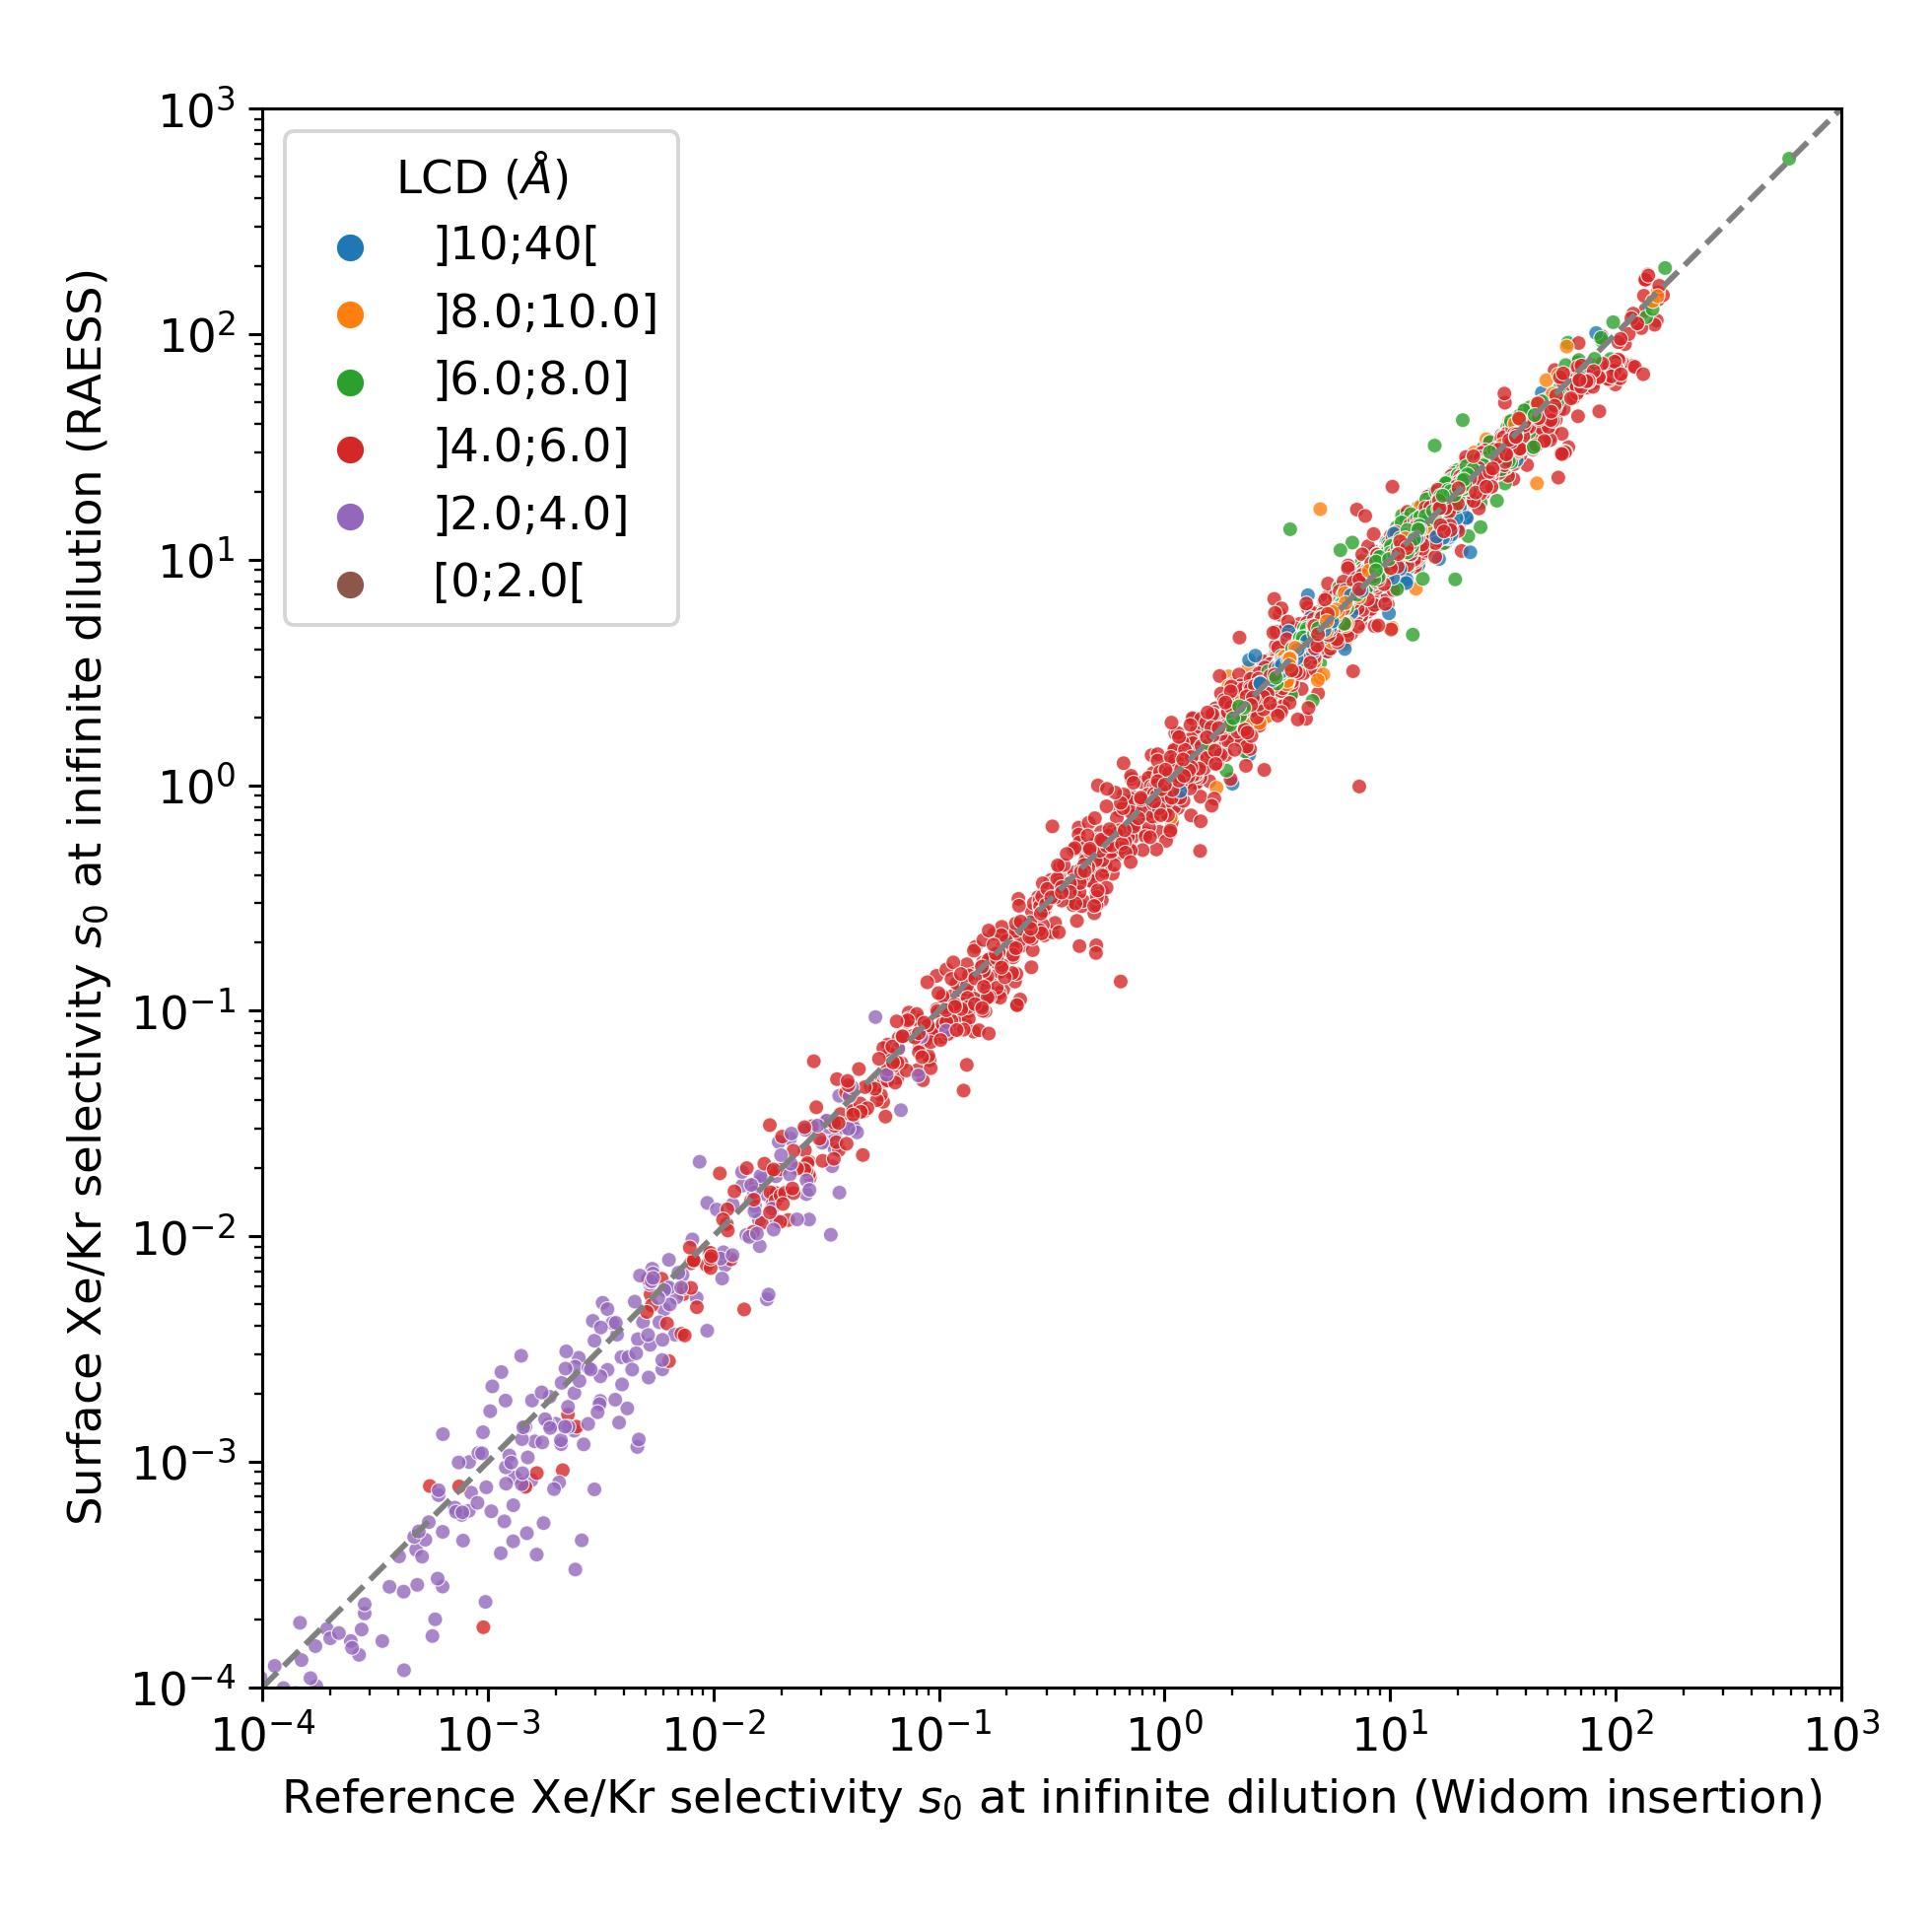
\includegraphics[width=0.5\linewidth]{figures/3-fastsim/s_0_widom_vs_s_0_surface_zoom.jpg}
  \caption{Scatterplot comparison of the Xe/Kr selectivity calculated by RAESS algorithm and the one calculated by the Widom insertion (in log scale) and labeled by the cavity size. }\label{fgr:s_0}
\end{figure}

To provide a thermodynamic interpretation, the exchange Gibbs free energy associated $\Delta\e{exch}G\e{0}\ex{Xe/Kr}$ with the selectivity defined in the previous chapter (equation~\ref{eq:exc_gibbs_free_energy}) can be utilized. By using this exchange Gibbs free energy, the assessment of the approach's performance becomes much more straightforward. The resulting RMSE is about \SI{0.36}{\kilo\joule\per\mole}. It is not possible to directly compare this error with the errors associated with adsorption enthalpy, as the ranges and interpretations differ significantly. In this case, selective materials exhibit a negative value of $\Delta\e{exch}G\e{0}\ex{Xe/Kr}$, ranging up to a maximum of approximately \SI{-12.7}{\kilo\joule\per\mole}. The relative error is naturally higher for the Gibbs free energy, which can be attributed to the increased uncertainty in the Henry constant and the denominator term introduced by krypton.

\begin{figure}[ht]
\centering
  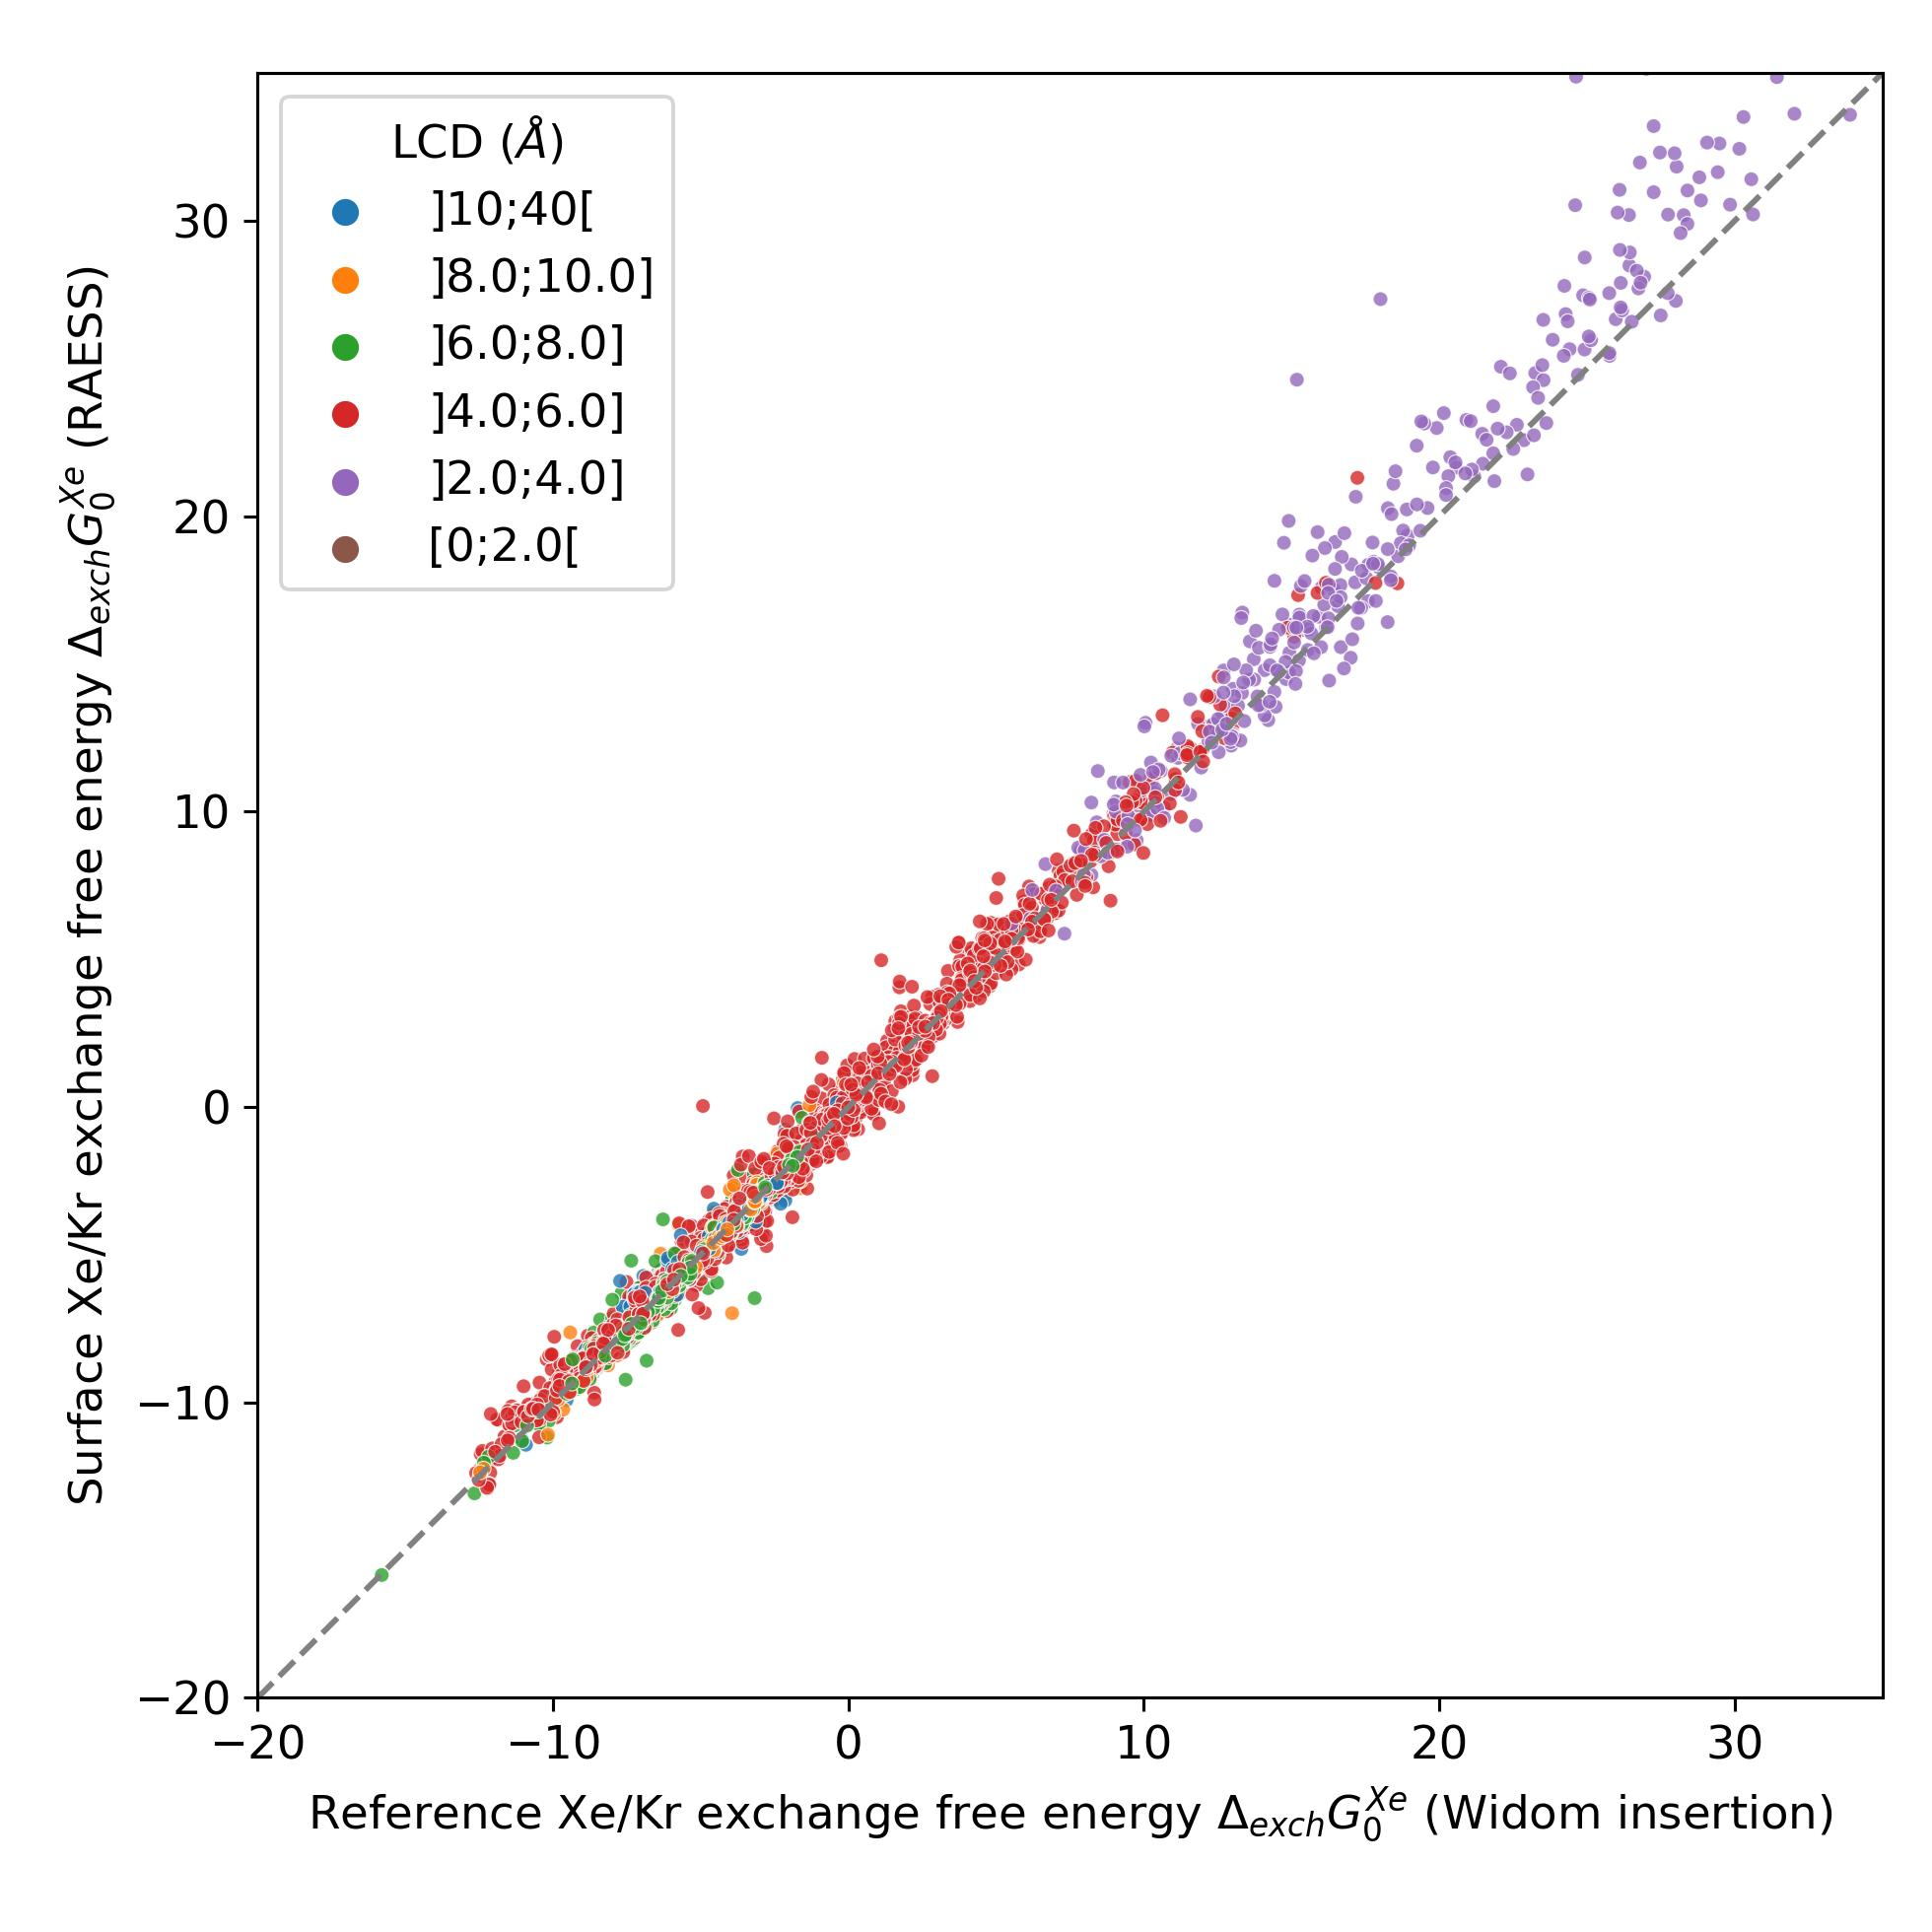
\includegraphics[width=0.5\linewidth]{figures/3-fastsim/G_XeKr_widom_vs_G_XeKr_surface_zoom.jpg}
  \caption{Scatterplot comparison of the exchange Gibbs free energy $\Delta\e{exch}G\e{0}\ex{Xe/Kr}$ calculated by the Widom insertion compared to the final implementation of RAESS (RMSE=\SI{0.36}{\kilo\joule\per\mole} and MAE=\SI{0.23}{\kilo\joule\per\mole}).}\label{fgr:exch_free_energy}
\end{figure}

To assess the performance of the RAESS algorithm in real scenarios, the top 100 most selective materials identified by RAESS and a Widom simulation (RASPA2) were compared in this study.  It was observed that 83 structures out of the top 100 materials identified by RAESS are also included in the top 100 materials obtained through Widom insertion. Although the correlation is not perfect, there will inevitably be some variation in the ordering of the top 100 materials provided by these two methods. The fact that {83\%} of the materials overlap indicates a relatively narrow difference. Expanding the comparison to the top 150 materials from the Widom simulation, it was found that 94 of them are present in the top 100 materials identified by the surface simulation. This suggests that the RAESS algorithm successfully identifies a a large majority of the top candidates obtained through the Widom insertion simulation.

\subsubsection{A Higher Temperature}

The RAESS method relies on the higher weight of the strong sites close to the surface of the pores. With an increase in temperature, the role of less attractive sites would become more significant, resulting in a decrease in the method's accuracy. To understand this limitation of the RAESS algorithm at higher temperatures, a comparison was made using the CoREMOF 2019 database.

\begin{figure}[ht]
\centering
  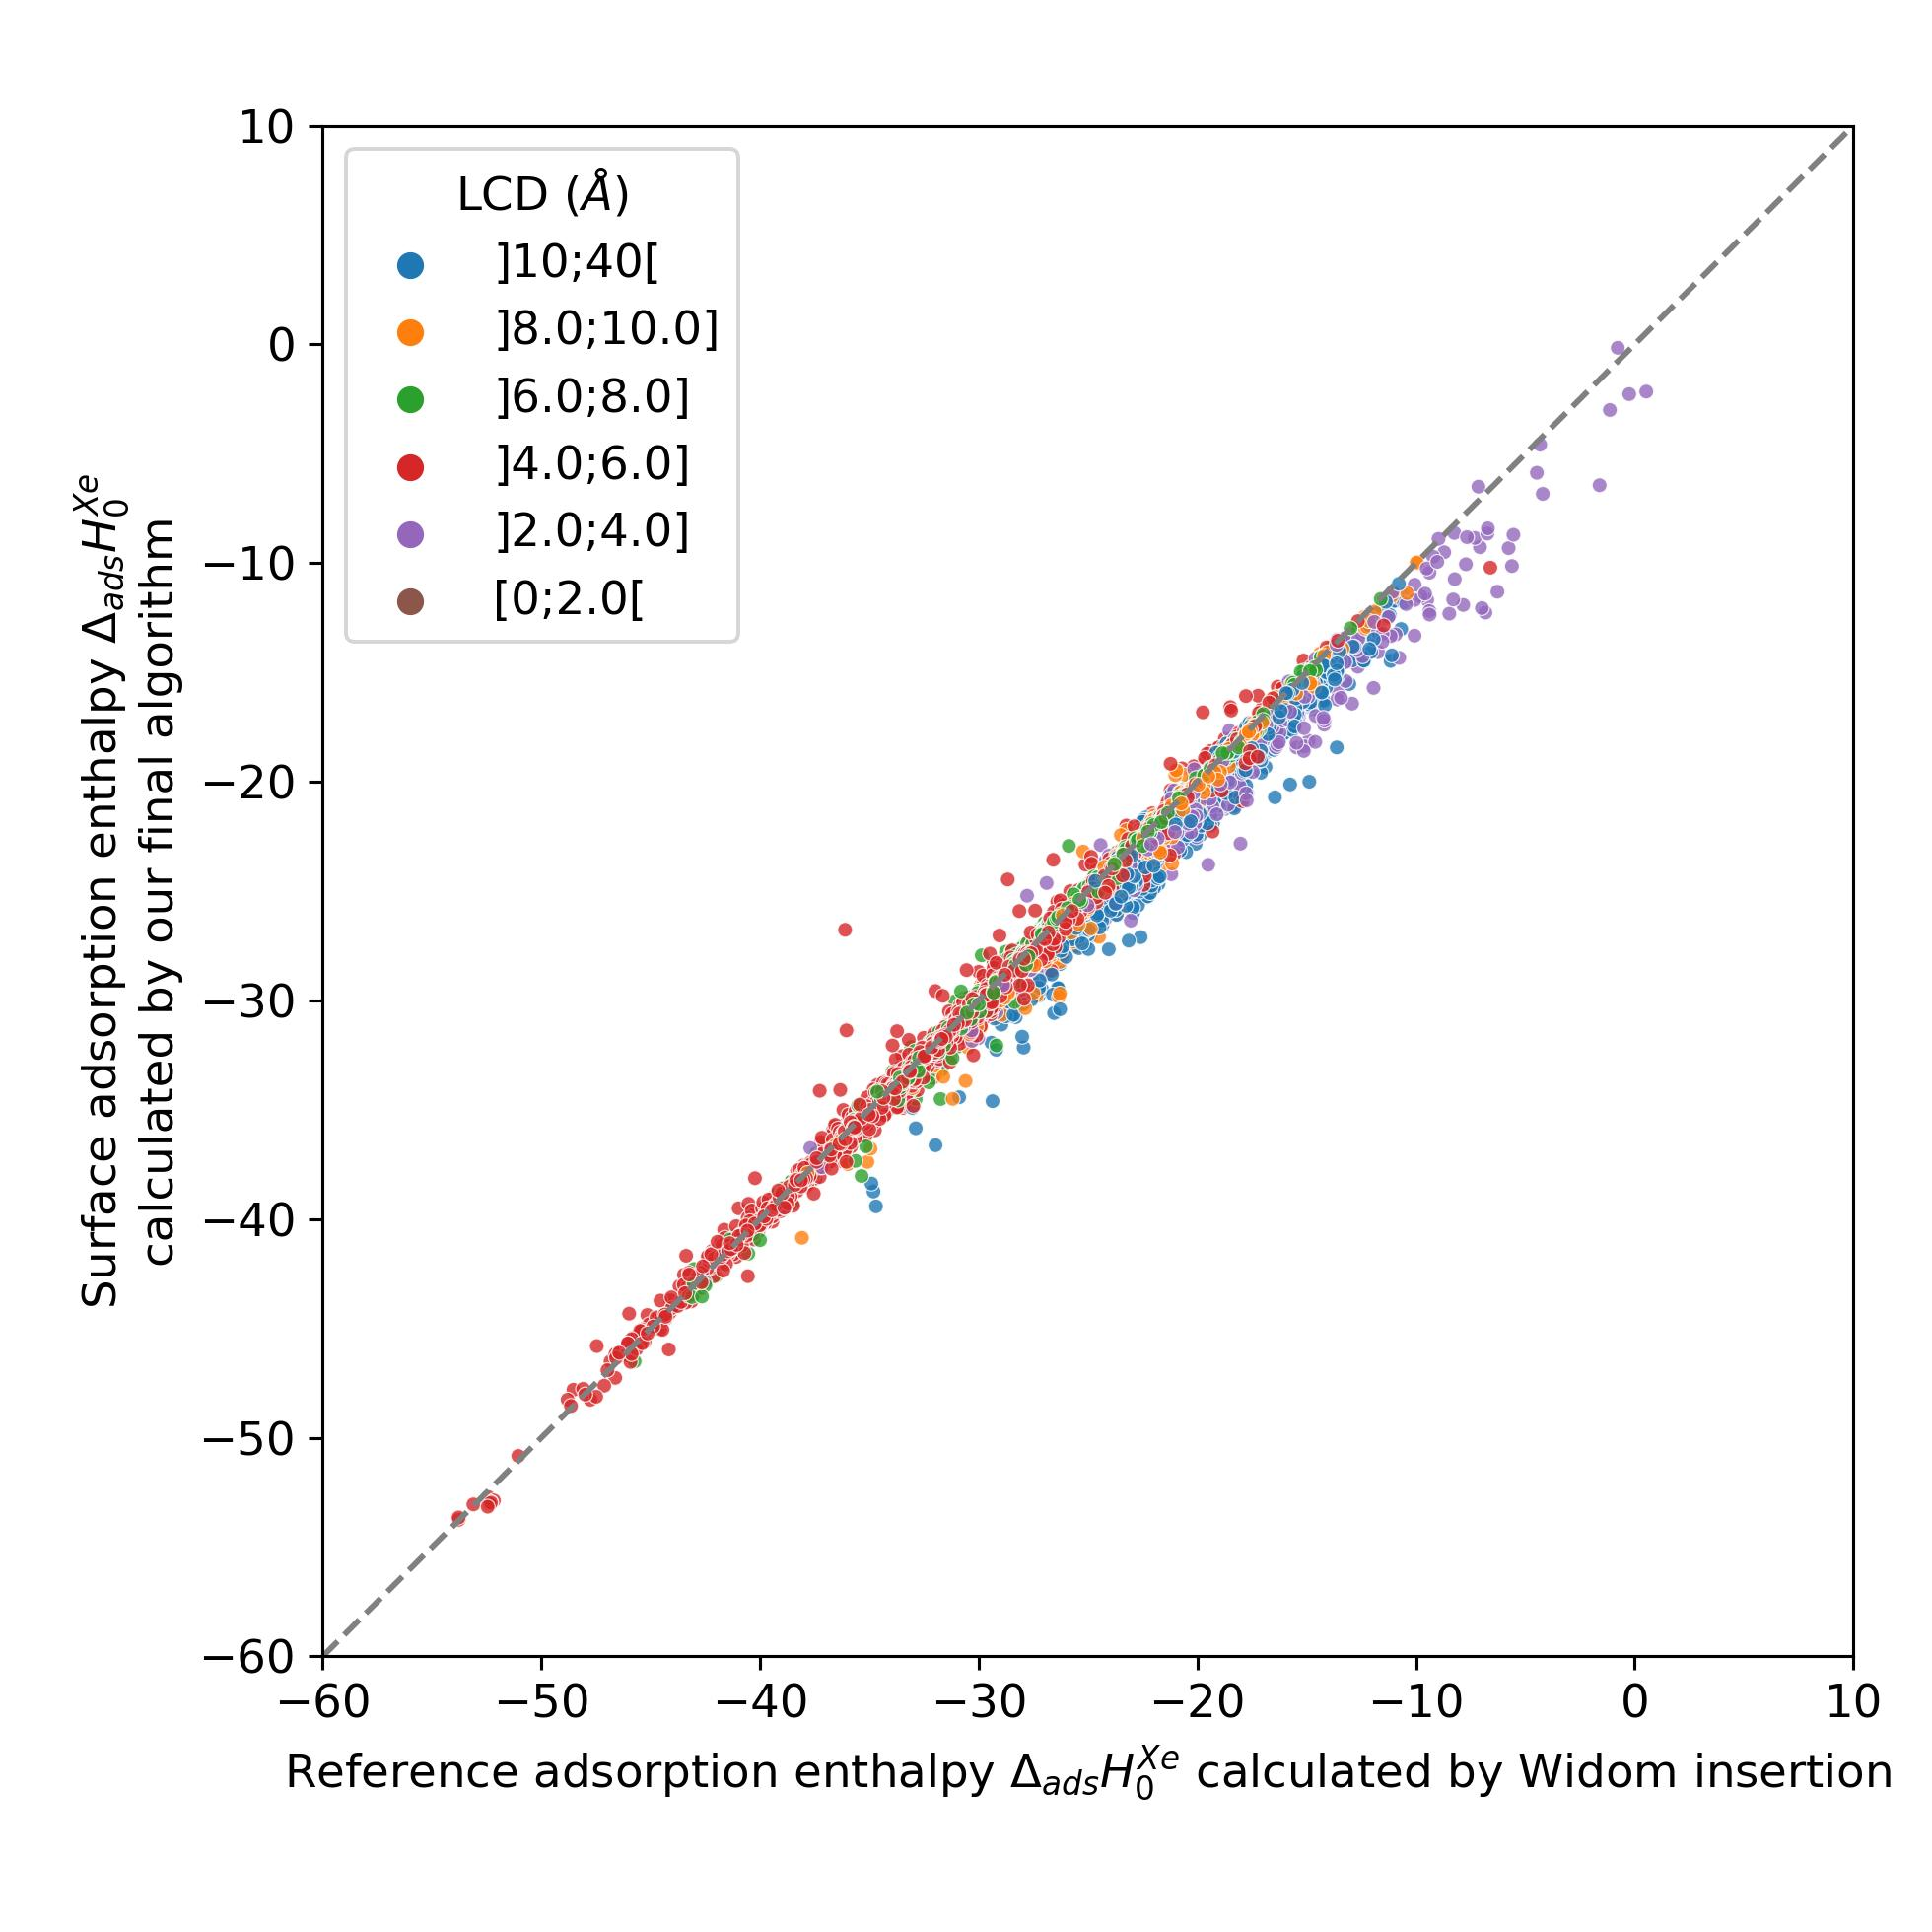
\includegraphics[width=0.5\linewidth]{figures/3-fastsim/H_Xe_widom_vs_H_Xe_surface_final_zoom_600K.jpeg}
  \caption{Scatterplot of the enthalpies calculated by our final algorithm ($\lambda=1.6$ and $\mu=0.85$) compared to the enthalpies calculated by a 12k step Widom insertion simulation of xenon in structures of CoRE MOF 2019 with LCD\e{CCDC} $\geq$ \SI{3.7}{\angstrom} at \SI{600}{\kelvin}. }
\end{figure}

As expected, the surface sampling method exhibits lower accuracy when subjected to Boltzmann averaging at higher temperatures. Nevertheless, it still demonstrates an acceptable correlation in performance, yielding an RMSE \SI{0.70}{\kilo\joule\per\mole} and a MAE of \SI{0.41}{\kilo\joule\per\mole}. The errors nearly doubled when the temperature was increased from \SI{298}{\kelvin} to \SI{600}{\kelvin}. However, these limitations of the method are not debilitating, as adsorption processes are typically not conducted at very high temperatures. High temperatures are commonly employed in temperature swing adsorption (TSA) for desorbing the adsorbates rather than adsorbing them.

\subsubsection{Other databases}\label{sct:other_database}

\textbf{ToBaCCo}

In this study, a total of 1,000 structures were randomly selected from the 13,511 porous frameworks within the ToBaCCo database to assess the robustness of the RAESS method on a database other than CoreMOF. Due to the presence of larger pores in the ToBaCCo structures, as indicated by Moosavi et al., these materials exhibit a higher degree of unfavorability towards the adsorption of small molecules (such as Xe). The correlation observed is relatively weaker compared to the CoRE MOF 2019 database. It is important to consider this reduced accuracy in light of the unsuitability of these materials for Xe/Kr separation. Moreover, it should be noted that points displaying weaker correlations correspond to those with an LCD\e{CCDC} greater than \SI{10}{\angstrom}, which is suboptimal for Xe-Kr separation.

\begin{figure}[ht]
\centering
  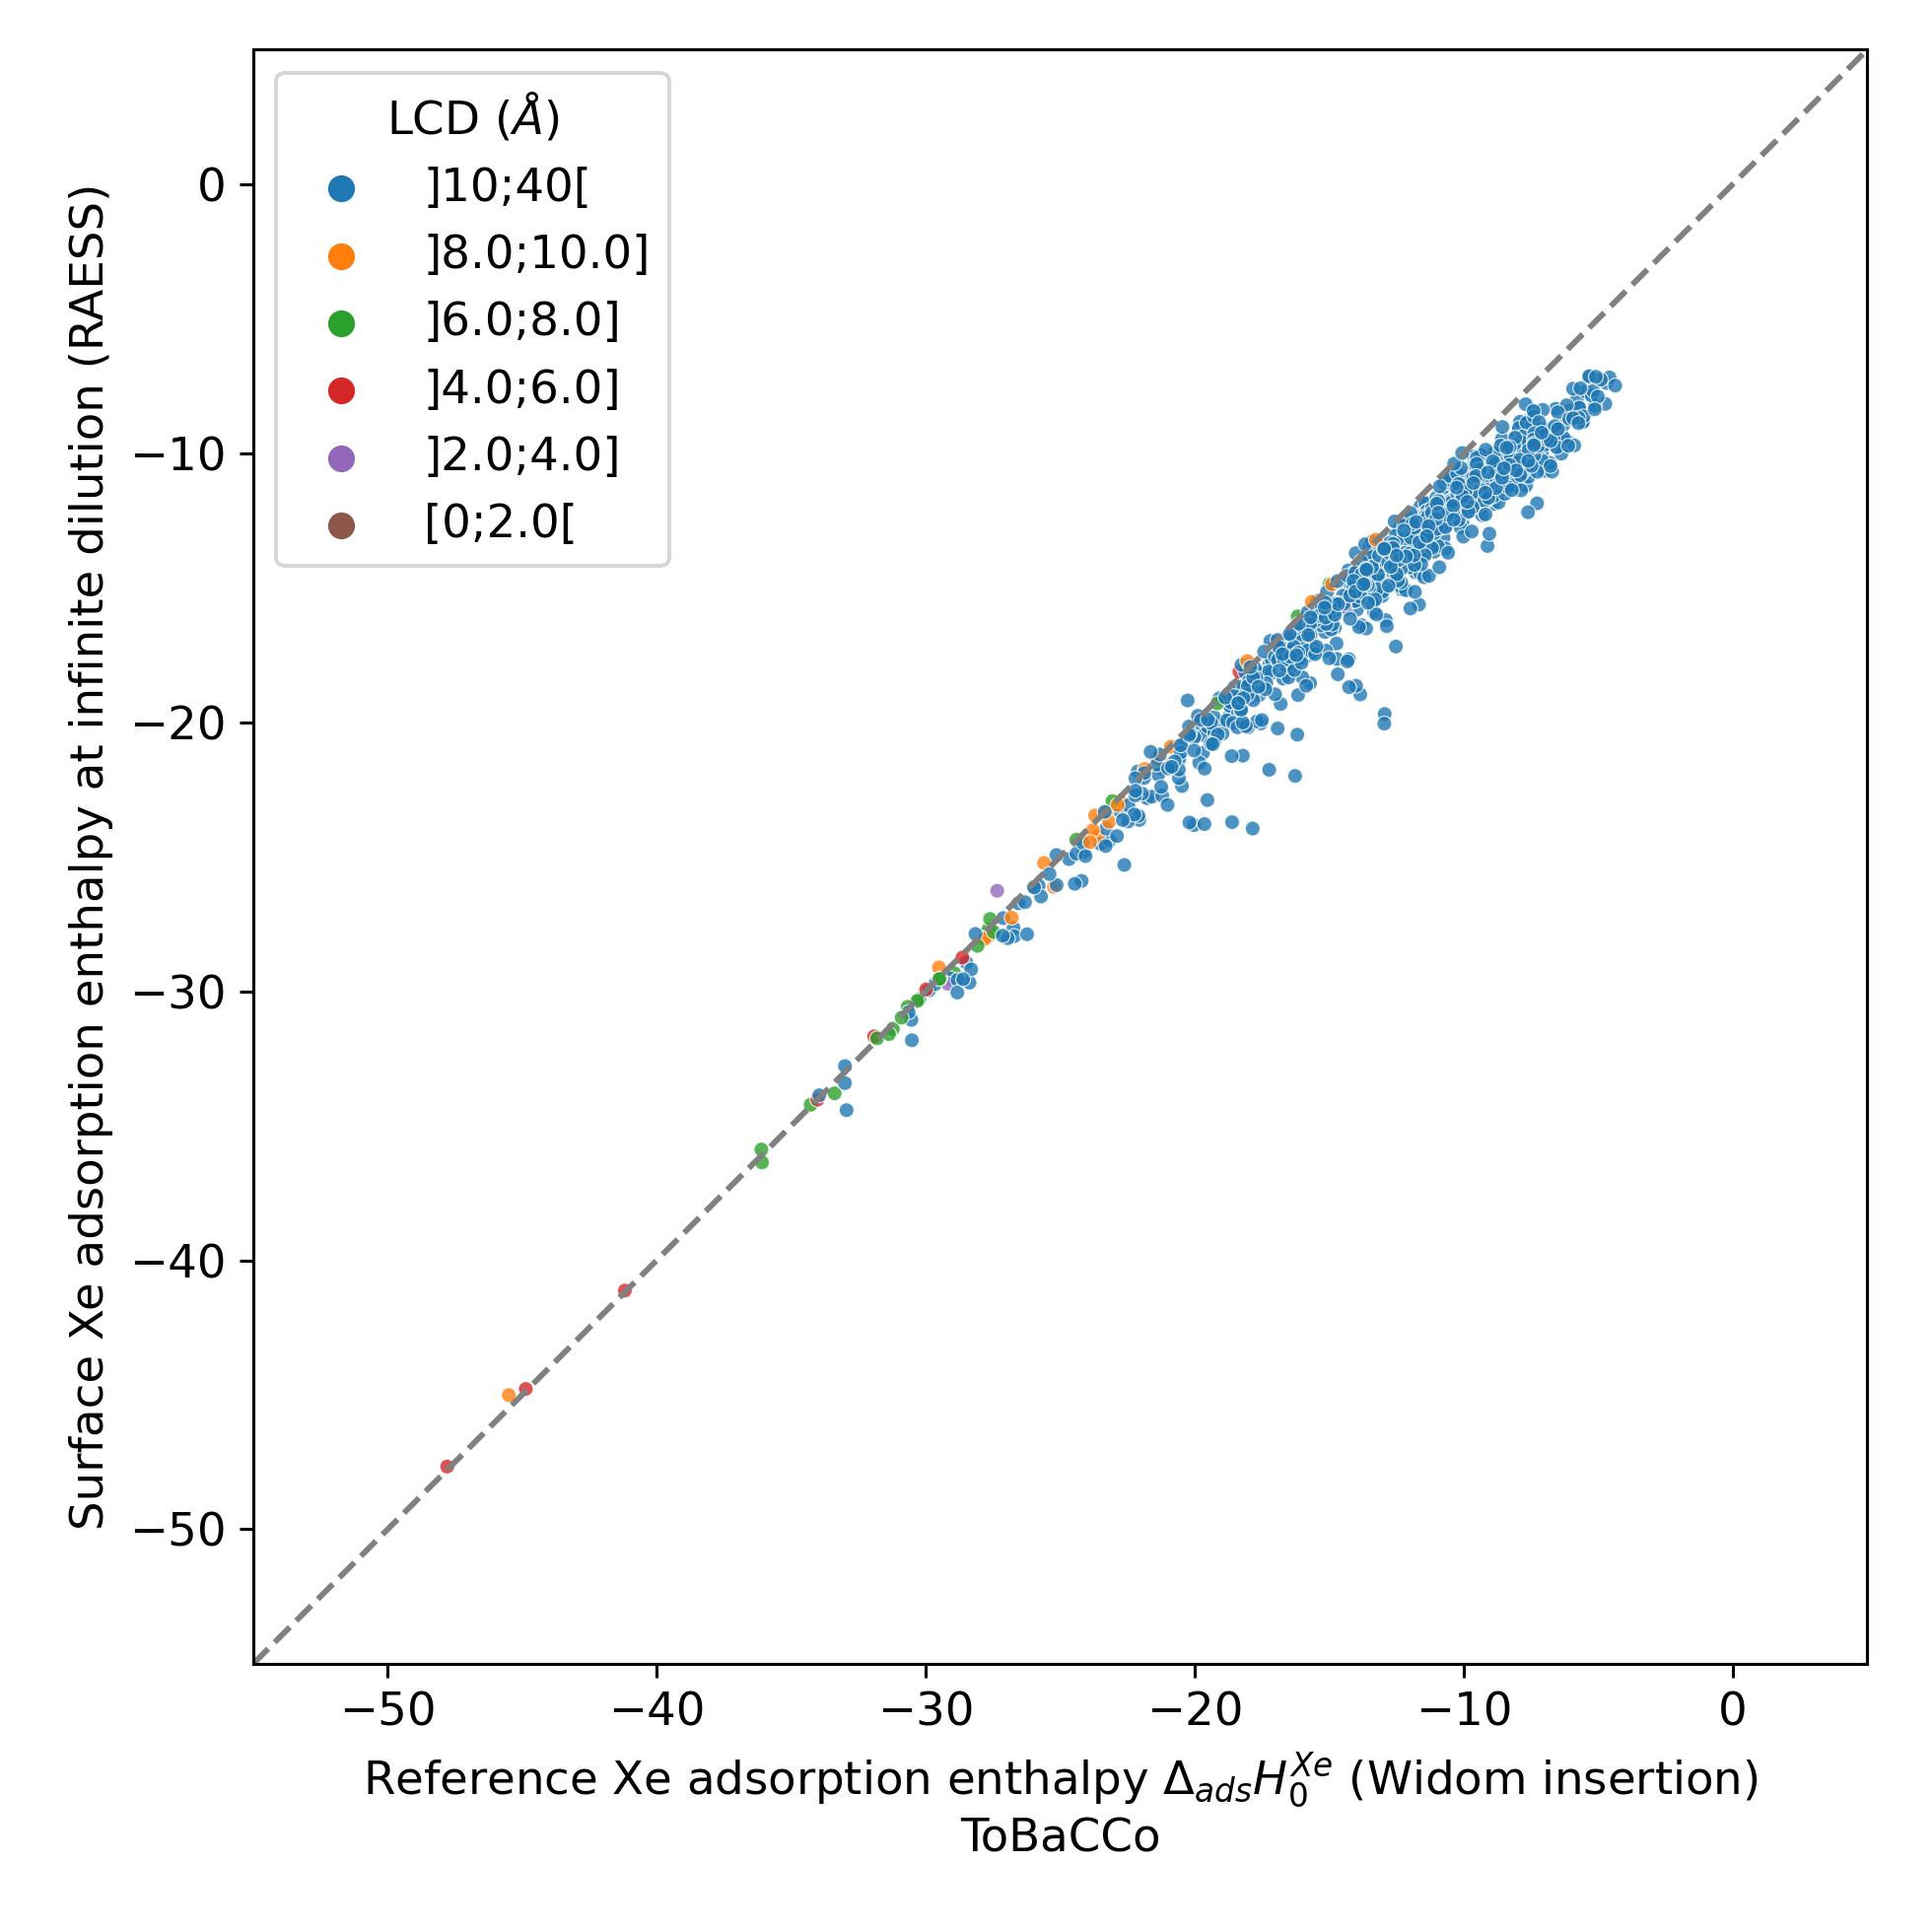
\includegraphics[width=0.5\linewidth]{figures/3-fastsim/H_Xe_0_widom_vs_Enthalpy_surface_kjmol_overview_tobacco.jpeg}
  \caption{Scatterplot comparison of the xenon adsorption enthalpy calculated by the RAESS algorithm and the Widom insertion (RASPA2) on the ToBaCCo database. RMSE = \SI{1.79}{\kilo\joule\per\mole} and MAE = \SI{1.48}{\kilo\joule\per\mole}. 915 structures have the LCD\e{CCDC} greater than \SI{10}{\angstrom}.}\label{fgr:tobacco}
\end{figure}

The algorithm demonstrates excellent performance when applied to highly adsorptive materials with xenon adsorption enthalpy values lower than \SI{-30}{\kilo\joule\per\mole}. This result is primarily due to the proximity of the adsorption sites to the material's surface. For broader pore sizes, some limitations of the methodology become apparent, and it is crucial to acknowledge them. These limitations do not significantly affect the final results when determining the most attractive materials. Moreover, it should be emphasized that this limitation does not have a significant detrimental effect, as the correlation, although weakened, remains intact and does not disappear.


\textbf{Amorphous materials}

To further extend the potential use cases of the RAESS algorithm, the amorphous database~\autocite{Thyagarajan_2020} was subjected to testing with the RAESS algorithm that found results for 176 structures out of 196. The RASPA2 software could not be executed on these amorphous structures with the computers used in this study that ran out of memory due to the large system size. Therefore, no comparison with a Widom simulation could be made. However, an alternative simulation method, which utilizes a homogeneously distributed grid sampled by an optimized algorithm presented in the next section, was employed. This grid sampling approach successfully computed the adsorption energies of 175 structures.

Table~\ref{tab:amorphous} presents the values of the adsorption enthalpies and Henry constants of selected amorphous materials, along with the corresponding computation times. The substantial number of atoms in each structure significantly increases the required CPU time compared to the crystalline structures of CoRE MOF 2019. Nonetheless, the time requirements remain manageable within a hypothetical screening procedure. Considering all 175 structures that were computable using our methods, the average time required per structure is approximately \SI{75}{\second}. 

\begin{table}[hb]
  \setlength{\extrarowheight}{1pt}
  \centering
  \begin{tabular}{|l|r|r|r|}
    \hline
    Structure Name & $\Delta\e{ads}H\e{0}\ex{Xe}$ (\SI{}{\kilo\joule\per\mole}) & $K\e{H}\ex{Xe}$ (\SI{}{\mole\per\kilo\gram\per\pascal}) & CPU time (s) \\
    \hline
    aCarbon-Marks-id035 &                 -63.55 &            6.98e-01 & 285.45 \\
    HCP-Colina-id016 &                 -30.61 &            8.85e-05 & 3.88 \\
    Kerogen-Coasne-id010 &                 -44.38 &            8.02e-03 & 61.2 \\
    PIM-Colina-id012 &                 -26.39 &            7.00e-05 & 8.86 \\
    \hline
    \end{tabular}
    \caption{Some amorphous materials' performance according to the RAESS algorithm. The results on the whole amorphous database is given in CSV format on the Github: \url{github.com/fxcoudert/citable-data/tree/master/154-Ren_ChemSci_2023}.}\label{tab:amorphous}
\end{table}

As shown in Figure~\ref{fgr:amorphous}, the accuracy of the surface sampling is desmontrated to be high, as evidenced by the highly similar results obtained through unbiased grid-based sampling. The RMSE is about \SI{0.83}{\kJ\per\mol}, which is higher than the one for CoRE MOF structures. This method has the potential to serve as a rapid screening tool for evaluating amorphous materials, especially considering the computational time required by the optimized grid sampling is about \SI{623}{\second}. The dimension reduction inherent to surface sampling makes it one order of magnitude faster than conventional techniques.

\begin{figure}[ht]
  \centering
  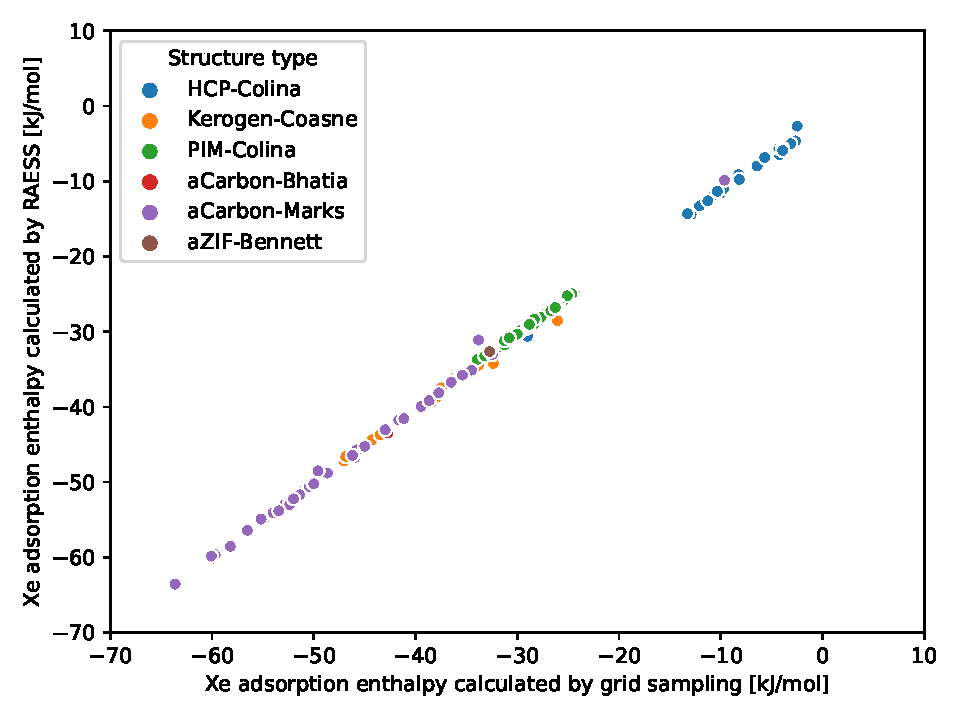
\includegraphics[width=0.5\linewidth]{figures/3-fastsim/amorphous_enthalpy.pdf}
  \caption{Scatterplot comparison of the xenon adsorption enthalpy calculated by the RAESS algorithm and the one calculated by a grid sampling (presented in the next section) on a database of porous rigid amorphous materials~\autocite{Thyagarajan_2020}. RASPA2 simulation could not be run on this database. Only the 175 structures computed by both methods are presented here. }\label{fgr:amorphous}
\end{figure}

\subsection{Perspectives of surface sampling}

A novel algorithm for the high-speed calculation of adsorption enthalpy in nanoporous materials has been described, employing a unique approach that significantly reduces the required sampling. Based on the core principle of dimensional reduction from a volume problem to a surface one, this algorithm outperforms the reference Widom insertion method (random sampling of porous space) in terms of both computational speed and accuracy, with an error on the order of \SI{0.4}{\kilo\joule\per\mole} observed across the entire CoRE MOF 2019 database for xenon adsorption. Furthermore, compared to existing fast sampling techniques such as Voronoi sampling, the surface sampling technique achieves similar CPU time requirements while offering better accuracy.

Based on these results, this algorithm has considerable potential for applications within current computational analysis workflows for material databases, particularly in high-throughput screening studies. For instance, it can be used to rapidly approximate the low-loading adsorption enthalpy of a molecule in nanoporous materials, allowing for the screening of structures with limited affinity for the target adsorbate molecule. It can also serve as a thermodynamic descriptor for selectivity prediction in machine learning models, as demonstrated by Simon et al.\autocite{Simon_2015} The computational speedup achieved by this novel methodology also enables the screening of larger-scale materials databases in the future.

It should be noted that the speed of the method primarily lies in the sampling technique itself, rather than the actual energy calculation. While the benchmarking in this work focused on a simple Lennard-Jones interaction potential, the surface sampling technique can equally be applied to accelerate samplings based on more computationally expensive modeling strategies, such as polarizable force fields or density functional theory (DFT) calculations. In the literature, the need for affordable \emph{ab initio} grade thermodynamic properties is is typically addressed by employing an importance sampling method based on a classical force.\autocite{Vandenbrande2018} In the method used in this study, the description of surface sampling remains independent of any force field, and the sampling spheres can be defined based on kinetic radius, van der Waals radius, or any other physically relevant distance. {As a result, given a definition of atomic radii, it is possible to define a surface on which other types of simulations, such as neural network potentials, DFT, or other force fields, can be conducted. While the accuracy and relevance of such sampling methods remain open questions, the approach undeniably accelerates simulations.} This acceleration could also be applied to the calculation of adsorption enthalpies while considering intrinsic structural flexibility,\autocite{Witman_2017} a task that is computationally demanding. As surface sampling is hundreds of times faster than standard methodologies, it becomes feasible to utilize hundreds of snapshots in flexibility-aware calculations.

Finally, although the algorithm in its present form can already be applied in a wide range of applications, there is potential for additional development work to generalize it to polyatomic adsorbates. For instance, {a definition of the molecular radius for non-spherical adsorbates and consideration} of the orientation conformation of the adsorbent would need to be addressed. {The distance to the surface could potentially depend on the orientation of the adsorbate or involve sampling a band volume on the surface. Although determining the best implementation of surface sampling for polyatomic adsorbates remains an open question, in theory, it should be feasible to apply it to more complex adsorbates than spherical noble gases.} This would add more complexity to the algorithm without altering the fundamental speedup achieved through surface sampling, as similar orientation moves are performed in other standard methodologies. To further improve accuracy, hybrid samplings with multiple sampling spheres or a combination of Voronoi nodes and sampling spheres could be tested. Another possibility is to incorporate fractions of spheres oriented towards the center of the pore defined by the Voronoi node. In theory, a wider variety of sampling points can only enhance the sampling process. Thus, there are multiple potential sampling techniques that could be developed based on the method introduced herein. {The code is made freely available on the group's GitHub (\url{github.com/coudertlab/RAESS}), where further development will be released.}

\textbf{Data Availability:} \url{https://github.com/fxcoudert/citable-data/tree/master/154-Ren_ChemSci_2023}

\section{Grid Adsorption Energies Descriptors (GrAED)}\label{sct:grid}

To conclude the overview of novel energy sampling methods, a revised version of the standard grid sampling will be presented. Grid sampling is the most accurate approach as it directly relies on the averaging definitions in equations~\ref{eq:eq:ads_enthalpy} and~\ref{eq:henry}. In this section,  the inherent symmetry operations of most material structures and the removal of framework occupied space will be leveraged to accelerate this typically slow method. This exhaustive approach allows for the calculation of energy distributions that are less biased compared to other methods. These energy distributions serve as fundamental building blocks for the prediction of ambient-pressure selectivity, which will be discussed in the next section.

\subsection{Implementation of an efficient grid algorithm}

To build more relevant energy descriptors, it is necessary to return to the definitions of adsorption enthalpy and Henry constant (equation~\ref{eq:ads_enthalpy} and~\ref{eq:henry}), as the latter require a homogeneous sampling of the adsorption space. The simplest way to achieve this consists in laying a grid in the 3D space. However, this method is known to be time-consuming in theory. Inspired by the work on surface sampling, an approach based on a symmetry-respecting grid was designed by leveraging algorithms from the Gemmi Project\autocite{Wojdyr_2022}. In this grid adsorption energy descriptor (GrAED) calculation algorithm, these new features, combined with grid sampling, significantly reduce the computational time required for adsorption energy calculations while maintaining high accuracy.

\begin{figure}[ht]
  \centering
    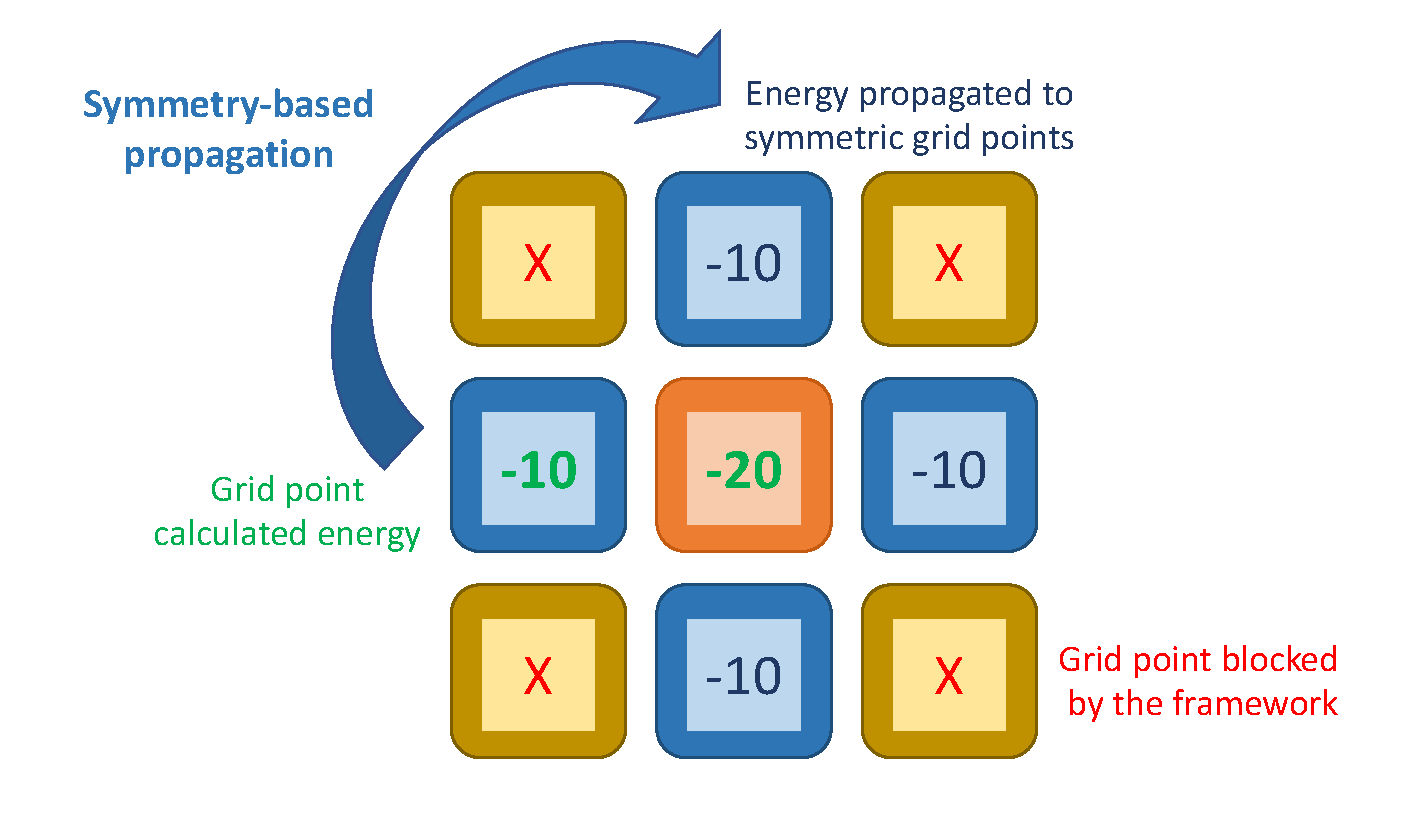
\includegraphics[width=0.5\textwidth]{figures/3-fastsim/grid_sampling.pdf}
    \caption{Principle of the energy sampling on a symmetry-based grid. On the 9 grid points, 4 points are blocked because they are too close to the framework atoms, 2 points are really calculated using the LJ potential and 3 points are propagated using the inner symmetry of the framework.}\label{fgr:principle_grid}
\end{figure}

The core structure of the corresponding algorithm encompasses a grid algorithm, where the evaluation of the interaction energy at each point of the preset grid over the structure's unit cell is required. A naive approach would demand an expensive energy calculation at each grid point. To improve this approach, two main simplifications are incorporated into the algorithm --- a quick evaluation of the framework occupied grid points and the exploitation of symmetry. The grid points that overlap with the framework's atoms have highly positive energy mainly due to the interaction with the overlapping atom. Contributions of high-energy values to the thermodynamic quantities presented in section~\ref{sct:thermo} are negligible. Hence, by employing a rejection parameter similar to the one developed for surface sampling introduced in section~\ref{sct:rejection_condition}, the interaction energy of the grid points within the sphere of radius $\mu\times\sigma_{g-h}$ can be precalculated. If the interaction energy value is higher than a preset energy threshold $E\e{th}$, the corresponding grid point adopts these values as the interaction energy, and no further calculation is performed for that point. The grid's symmetry is determined based on the structure's symmetry using the Grid definition of the Gemmi Project. Through the utilization of symmetry operations on a grid point value, it can be propagated to other symmetry-equivalent grid points, as illustrated in Figure~\ref{fgr:principle_grid}. This approach reduces the computation time required to calculate the interaction energy of a guest molecule at a given grid node with all the surrounding framework atoms within a specified cutoff. Having presented the primary components of our optimized grid calculation, the integration of this calculation in the algorithm's implementation will now be demonstrated.

\begin{enumerate}
  \item A loop performed over the framework atoms and the grid points around a sphere of radius $\mu\times\sigma_{g-h}$, where $\sigma_{g-h}$ is the distance at which the LJ potential energy between the guest atom $g$ and the host atom is zero. The LJ potential energy between the guest molecule and the closest host atom is calculated and only the grid points with an energy lower than a predefined threshold $E\e{th}$ are considered ``unvisited'' and will be recalculated in the following loop, the others are considered blocked by the framework and will be considered already ``visited''. This first loop over the framework atoms aims at filtering out the grid points that are blocked by the framework, and this preliminary filtering will be referred to as ``blocking'' in the Table~\ref{tab:grid}.
  \item A second loop over the ``unvisited'' grid points is performed --- at each increment, if the point is ``unvisited'', the interaction energy is calculated between the guest and all the host atoms within the cutoff, then the symmetric images of this point are filled with the same energy value and are considered ``visited'' by the algorithm. This symmetry-aware grid exploration allows the algorithm to divide the time required by the average number symmetry images --- this module will be referred to as ``symmetry'' on Table~\ref{tab:grid}.
\end{enumerate}

A ``fast'' version of the grid calculation algorithm was built by combining both the ``blocking'' of the high energy grid points and the ``symmetry'' based calculation of the interaction energies. This algorithm, which can compete with the previously developed rapid surface sampling method (RAESS), was built. The spacing between the grid points can be adjusted to control the trade-off between accuracy and computation time, with the computation time theoretically inversely proportional to the cube of the spacing. Interestingly, for certain spacing values, this algorithm can even outperform surface sampling on the CoRE MOF database, where symmetry plays a significant role (see Table~\ref{tab:grid}). The full implementation of the GrAED algorithm can be found at the following Github url: \url{github.com/coudertlab/GrAED.git}.

\subsection{Performance on the adsorption equilibrium}

When considering the performance of this new grid sampling algorithm in comparison to previously introduced sampling algorithms, the utilization of this new sampling technique on the CoRE MOF 2019 database proves to be highly advantageous due to its accuracy and speed. The efficient time performance of the grid sampling on the structures within the CoRE MOF 2019 database can be attributed to the relatively small porosity of the materials and their high degree of symmetry. For example, the average void fraction for a \SI{1.2}{\angstrom} probe radius is equal to $0.16$, while the average number of symmetric images is $5.8$ (most MOFs present symmetry operations). As a result of the ``blocking'' procedure, only approximately {$\sim$16\%} of the grid points necessitate actual calculation on average. Additionally, the ``symmetry'' procedure ensures that only around {$\sim$17\%} of points need to be considered. The combination of both procedures significantly reduces the number of relevant points to merely {2.7\%} of the grid. This reduction substantially decreases the CPU time required for the calculation while maintaining a satisfactory level of accuracy (with a low error on the Xe adsorption enthalpy of \SI{0.014}{\kilo\joule\per\mole}) compared to the naive grid approach, as shown in Table~\ref{tab:grid}. With the blocking procedure in the grid simulation, the time required is reduced by {$\sim$70.6\%} when compared to the naive approach, and a similar reduction of {$\sim$76.6\%} is observed for the symmetry-aware grid sampling. By combining both simplifications, the fast grid sampling technique achieves a time reduction of nearly {$\sim$91.6\%} for a grid spacing of \SI{0.12}{\angstrom}, aligning with the aforementioned decreased number of sampled points.

\begin{table}[ht]
  \centering
  \setlength{\extrarowheight}{1pt}
  \begin{tabular}{|l|r|r|}
    \hline
    Energy sampling  & RMSE on xenon  &  Average CPU  \\
    method  & adsorption enthalpy (\si{\kilo\joule\per\mole}) &  time (s) \\[0.5mm]
    \hline
    Grid -- naive -- \SI{0.12}{\angstrom} & 0.014  &  35.4 \\[0.5mm] 
    Grid -- blocking -- \SI{0.12}{\angstrom} & 0.014  &  10.4 \\ 
    Grid -- symmetry -- \SI{0.12}{\angstrom} & 0.014  &  8.3 \\ 
    Grid -- fast -- \SI{0.12}{\angstrom} & 0.014  &  2.96 \\
    Grid -- fast -- \SI{0.2}{\angstrom} & 0.048  &  0.41 \\
    Grid -- fast -- \SI{0.3}{\angstrom} & 0.21  &  0.13 \\
    Voronoi sampling &   2.1  & 0.40 \\
    RAESS\autocite{Ren_2023} & 0.33   &  0.34 \\
    Widom\autocite{Widom1963} (12k cycles) & 0.038  &  150 \\
    \hline
  \end{tabular}
  \caption{Performance comparison of the new grid method to other standard techniques used to calculate the xenon adsorption enthalpies. The RMSE is calculated by comparing to the values given by a 100k-step Widom insertion considered as the ground truth. The associated calculations are performed on the structures with the LCD\e{CCDC} over \SI{3.7}{\angstrom} of CoRE MOF 2019 database with a single Intel Xeon Platinum 8168 core at 2.7~GHz. The GrAED algorithm (with$\mu=0.8$ $E\e{th}=$\SI{100}{\kilo\joule\per\mole}) is evaluated at different grid spacings ($0.12$, $0.20$, $0.30$).}\label{tab:grid}
\end{table}


\begin{figure}[ht]
  \centering
    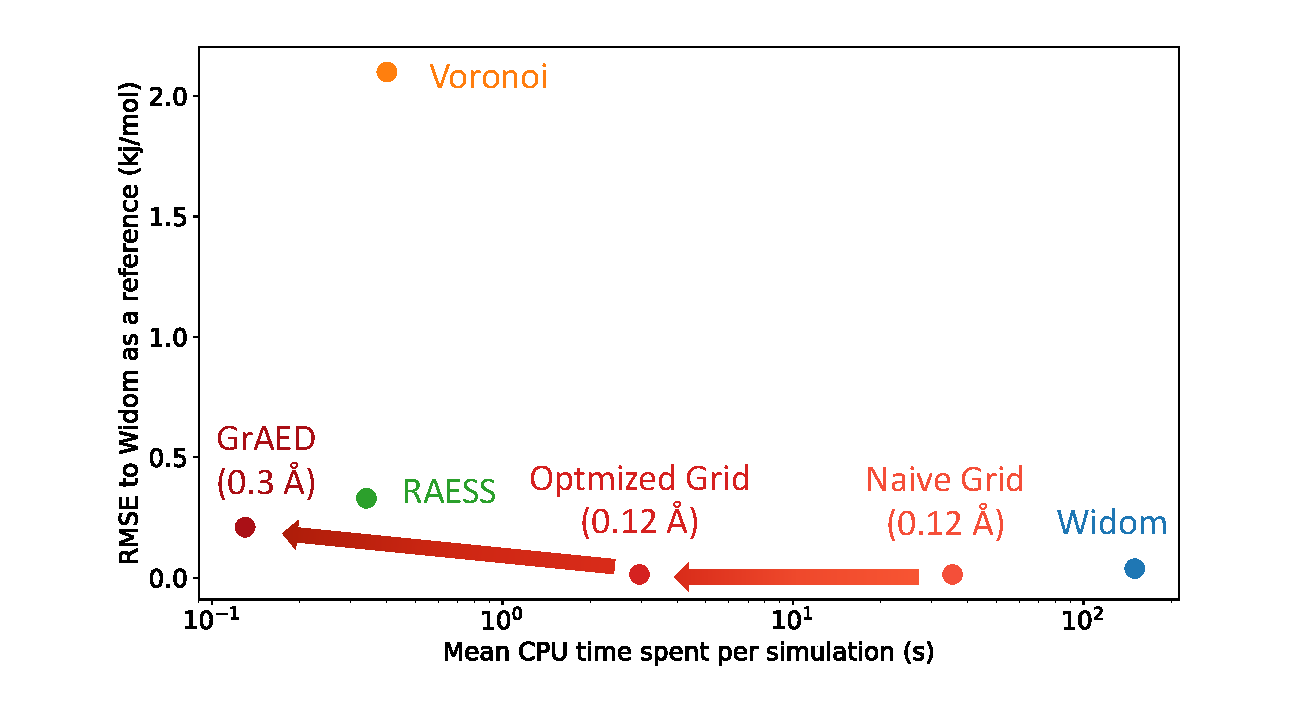
\includegraphics[width=0.7\textwidth]{figures/3-fastsim/Grid_sumup.pdf}
    \caption{Comparison of the RMSE on Xe adsorption enthalpy and the average CPU time required to run a simulation on a structure of CoRE MOF 2019 (LCD\e{CCDC} $\geq$ \SI{3.7}{\angstrom}). The values are the same as in the Table~\ref{tab:grid}. }\label{fgr:grid_perfomance}
\end{figure}

As shown in Figure~\ref{fgr:grid_widom}, the accuracy of the adsorption enthalpy and the Henry constant is not compromised by the approach. An almost perfect agreement between the Widom insertion method and the grid-based approach can be observed when utilizing a finely meshed grid (\SI{0.12}{\angstrom} spacing). This alignment was expected since both methods involve unbiased sampling of adsorption energies. The figure reveals minimal error in both adsorption enthalpy and Henry constant. The RMSE on the adsorption enthalpy is only about \SI{0.01}{\kilo\joule\per\mole}, while the RMSE on the log10 of the Henry constants (in \si{\milli\mole\per\gram\per\pascal}) is also extremely low, at $0.01$. This method adheres to the initial definition of these quantities at infinite dilution, explaining the unsurprising nature of this perfect correspondence.

\begin{figure}[ht]
  \centering
    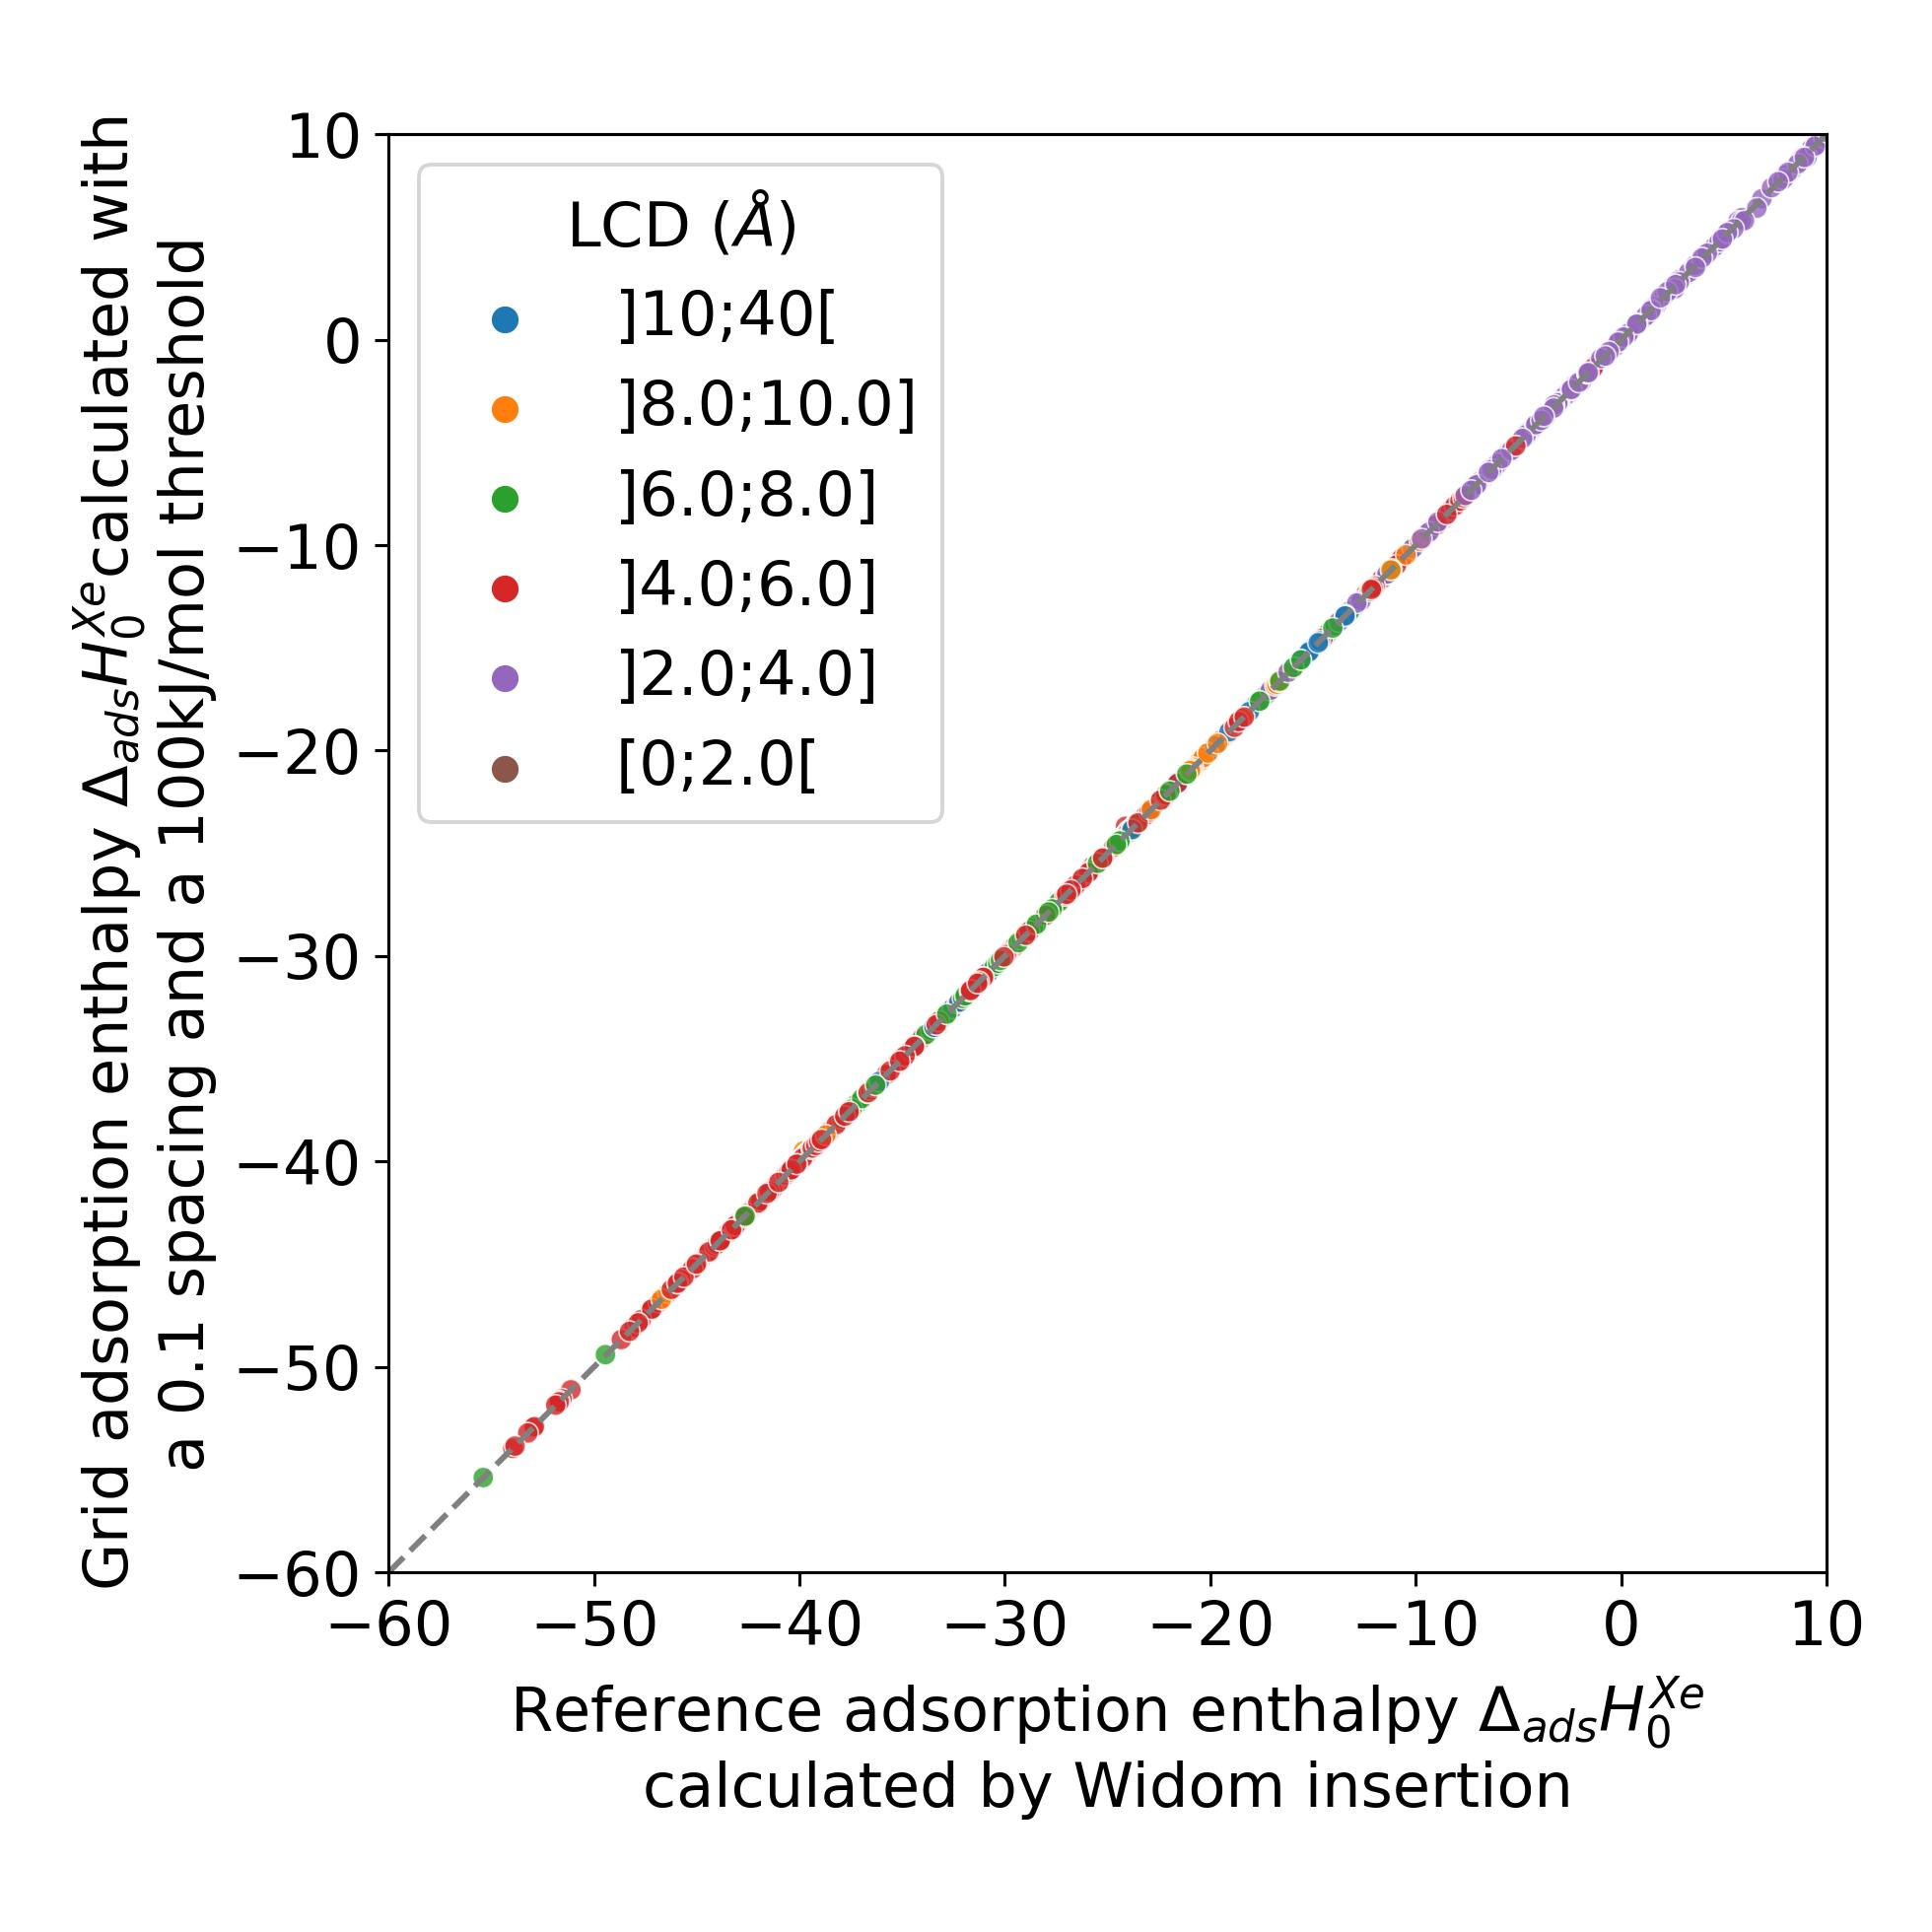
\includegraphics[width=0.45\textwidth]{figures/3-fastsim/H_Xe_widom_vs_H_Xe_grid_overview.jpg}
    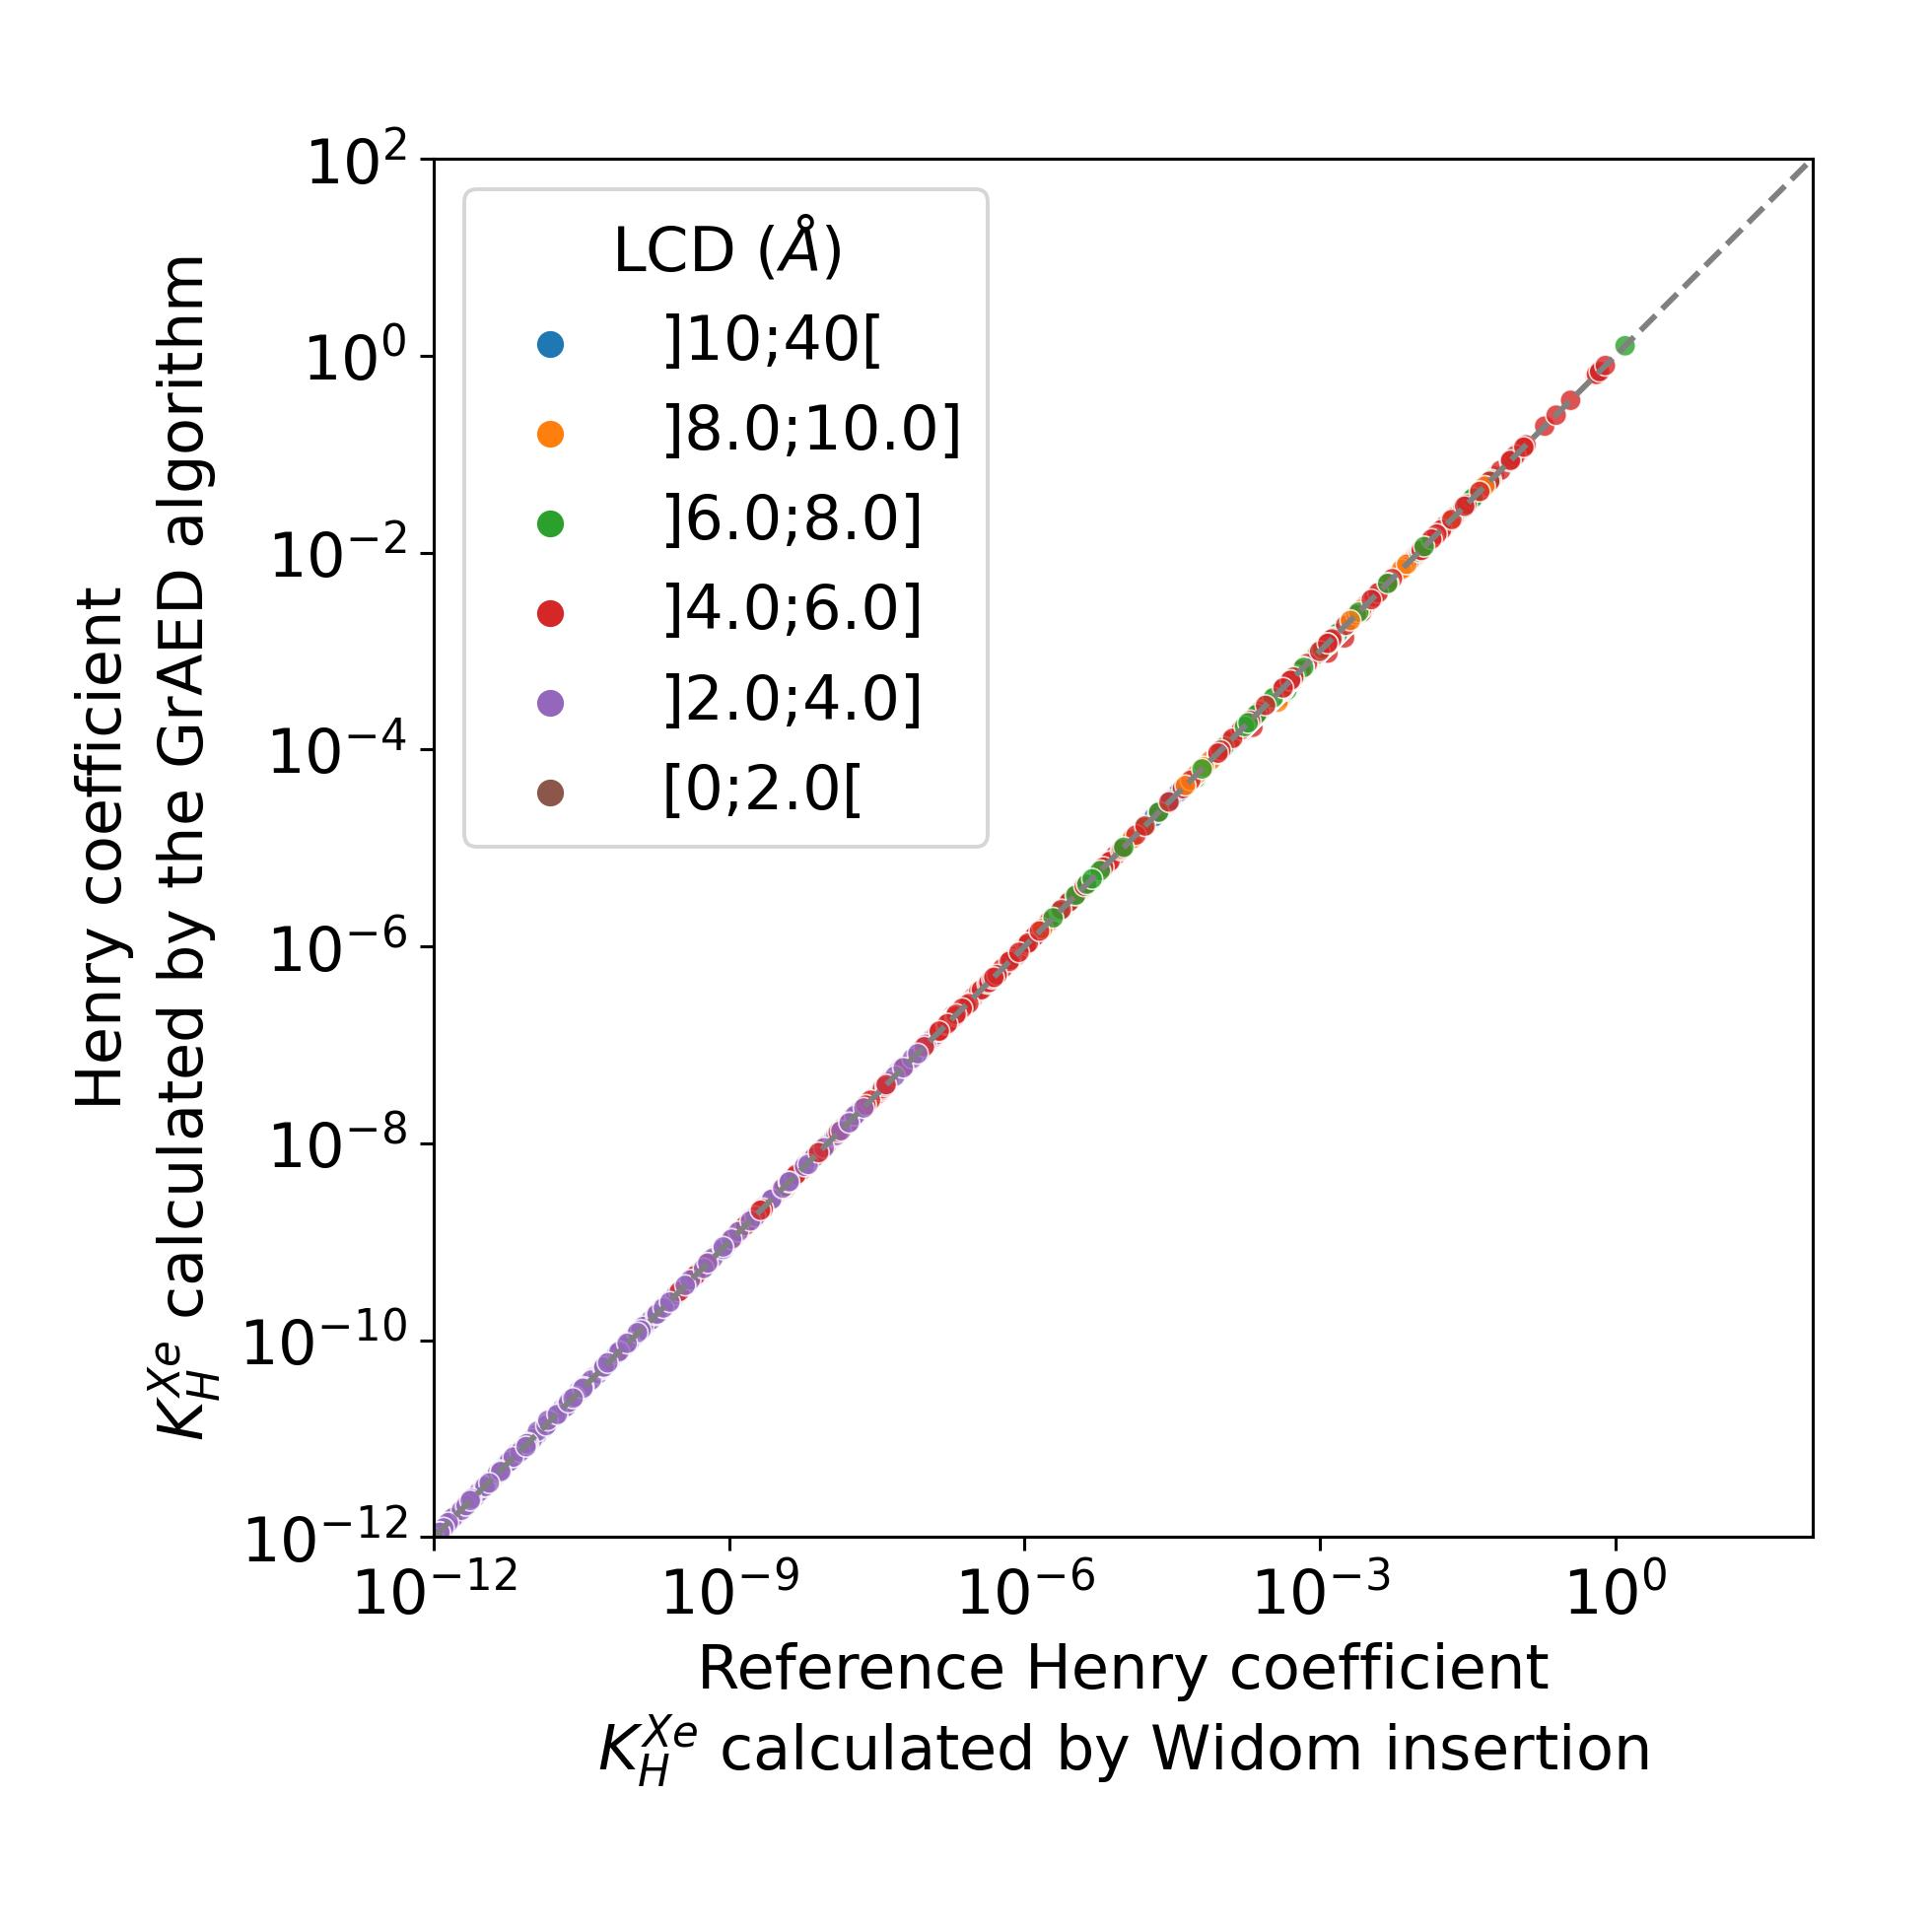
\includegraphics[width=0.45\textwidth]{figures/3-fastsim/K_Xe_widom_vs_K_Xe_grid_overview.jpg}
    \caption{Comparison of the xenon adsorption enthalpies (left) and the Henry constants (right) calculated by the optimized grid energy sampling (for a \SI{0.12}{\angstrom} spacing, a rejection parameter $\mu=0.8$ and an energy threshold $E\e{th}$ of \SI{100}{\kilo\joule\per\mole}) and by the Widom insertion of RASPA2 with 100,000 cycles on the CoRE MOF 2019 structures (LCD\e{CCDC} $\geq$ \SI{3.7}{\angstrom}). }\label{fgr:grid_widom}
\end{figure}

The little computation time required to achieve such an accuracy, however, is much more interesting. When examining the Table~\ref{tab:grid}, it can be observed that the highly accurate grid sampling approach attains a similar level of accuracy as a 12k-cycle Widom insertion calculated using the RASPA2 software, but it is 50 times faster. On the CoRE MOF 2019 database, by utilizing a less stringent grid spacing of \SI{0.3}{\angstrom}, the GrAED algorithm may even be more interesting than the RAESS algorithm, as it reduces the computation time by half while maintaining slightly higher accuracy. This highly comparable performance to a dimensionally reduced sampling technique can be attributed to two factors of the CoRE MOF database. Firstly, the structures have smaller pores, resulting in a higher surface-to-volume ratio, which increases the computation time for RAESS. Secondly, the highly symmetric nature of CoRE MOF structures significantly reduces the computation time required for GrAED, which is not the case for other databases such as ToBaCCo or the amorphous database previously examined in section~\ref{sct:other_database}. 

For instance, on the amorphous database (see section~\ref{sct:other_database}), the computation time for grid sampling is found to be 750 times longer compared to surface sampling, with an RMSE of only \SI{0.83}{\kJ\per\mol}. In the case of amorphous databases, surface sampling outperforms exhaustive grid sampling due to the minimal reduction in the number of sampled points caused by symmetry and overlap considerations, thereby showcasing the greater impact of dimensionality reduction achieved through surface sampling. In the ToBaCCo database,\autocite{Colon_2017} where symmetry no longer plays a significant role and the pores are larger, resulting in fewer points obstructed by the framework, the performance of grid sampling is directly affected when compared to the RAESS algorithm. The average time required for the thousand structures in ToBaCCo, as considered in section~\ref{sct:other_database}, is now \SI{735}{\s}, in contrast to less than \SI{2}{\s} for surface sampling. By increasing the grid spacing to $0.3$, a computational time reduction to approximately \SI{47}{\s} can be expected (deduced using a rule of three). However, the accuracy is significantly higher than that of surface sampling (see Figure~\ref{fgr:grid_tobacco}), reaching an extremely low RMSE of \SI{0.02}{\kJ\per\mol}. Depending on the number of structures and their nature (symmetry, porosity), wthe selection between the more efficient yet less accurate RAESS and the GrAED software must be made.

\begin{figure}[ht]
  \centering
    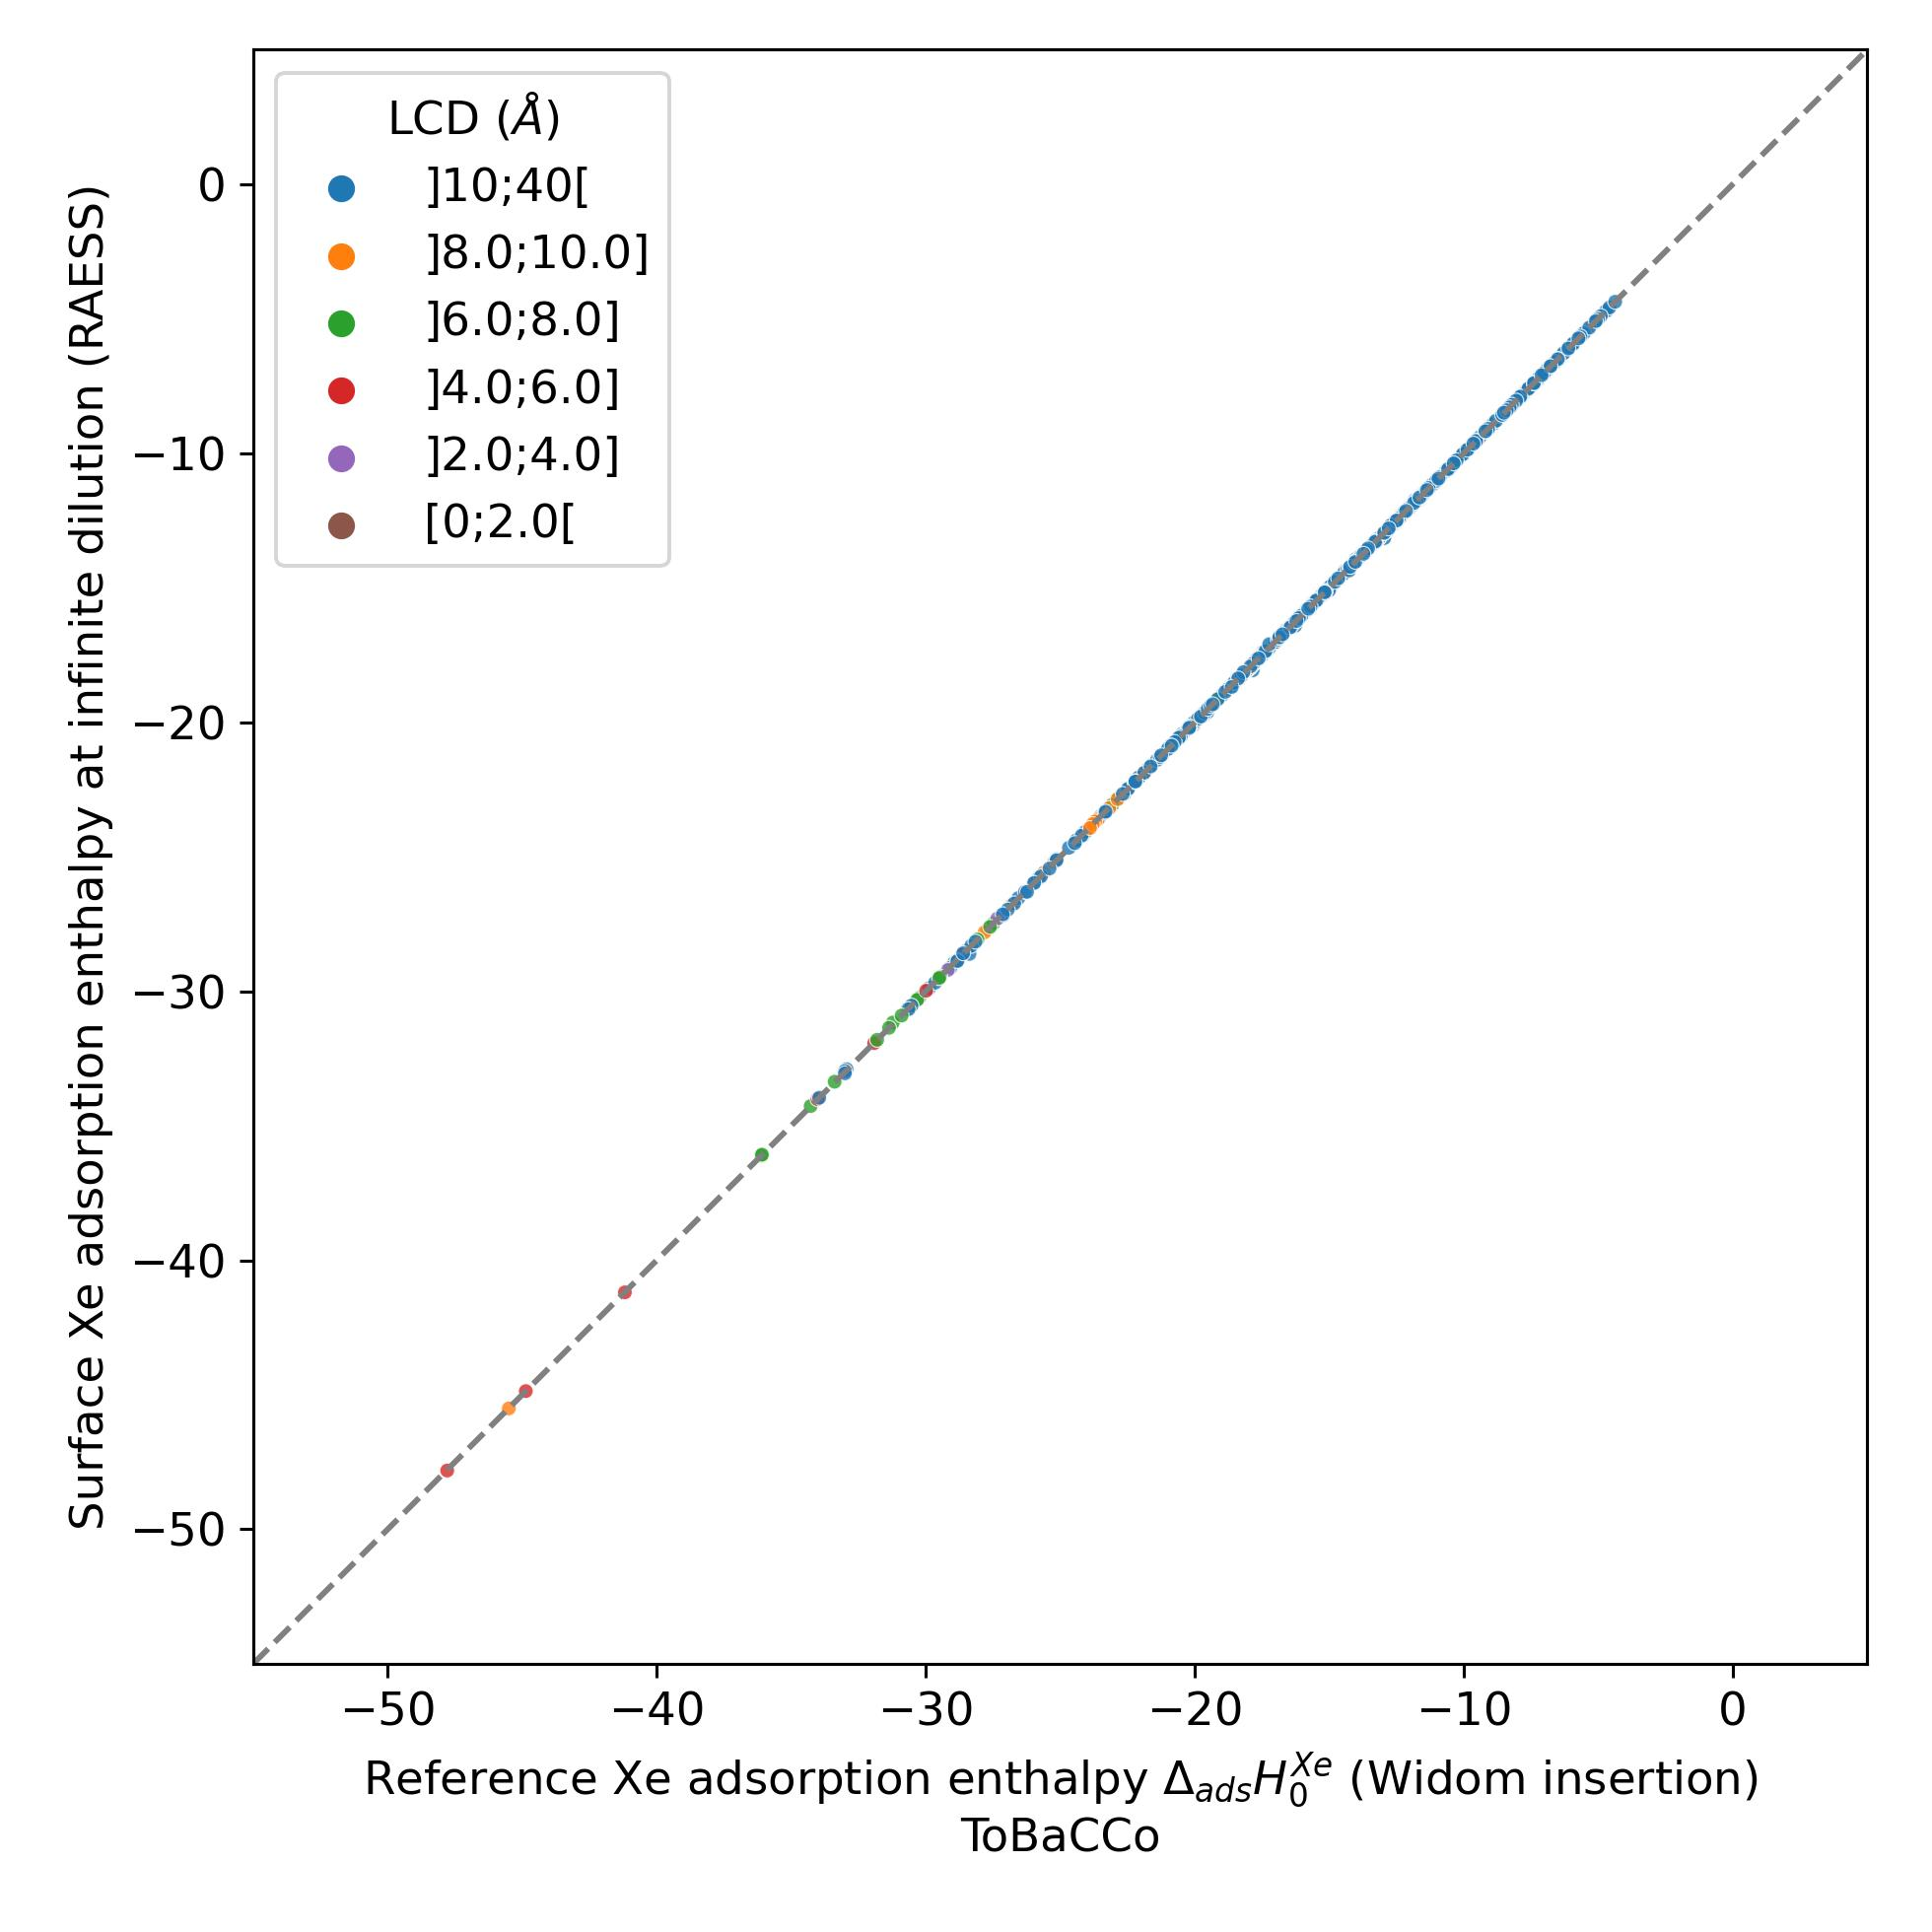
\includegraphics[width=0.45\textwidth]{figures/3-fastsim/H_Xe_0_widom_vs_Enthalpy_grid_kjmol_overview_tobacco.jpeg}
    \caption{Comparison of the xenon adsorption enthalpies (left) and the Henry constants (right) calculated by the optimized grid energy sampling (for a \SI{0.12}{\angstrom} spacing, a rejection parameter $\mu=0.8$ and an energy threshold $E\e{th}$ of \SI{100}{\kilo\joule\per\mole}) and by the Widom insertion of RASPA2 with 100,000 cycles on 1000 randomly selected structure of the ToBaCCo.\autocite{Colon_2017} }\label{fgr:grid_tobacco}
\end{figure}

From the energy values of this grid, a multitude of valuable descriptors for the adsorption process can now be calculated. The performance has been assessed for Xe adsorption enthalpy and Xe Henry constant, as discussed in section~\ref{sct:thermo}. Additionally, the Xe adsorption Gibbs free energy and Xe adsorption entropy can be derived. With the inclusion of krypton alongside xenon, the thermodynamic quantities for Kr adsorption can be naturally evaluated. Furthermore, the exchange thermodynamic quantities, particularly the Xe/Kr selectivity (the key metric for assessing the separation process of interest), can also be determined.


\subsection{Performance on the exchange equilibrium}

The Xe/Kr selectivity is commonly used to characterize the competitive adsorption of a binary mixture of xenon and krypton. Unlike a single-component metric such as the Henry constant, the relative uncertainty in the selectivity inherently increases since it involves the quotient of the Henry constants of the competitive adsorbates. In this section, the objective is to quantify this error and determine its relevance in characterizing the separation using the optimized grid sampling method.

\begin{figure}[ht]
  \centering
    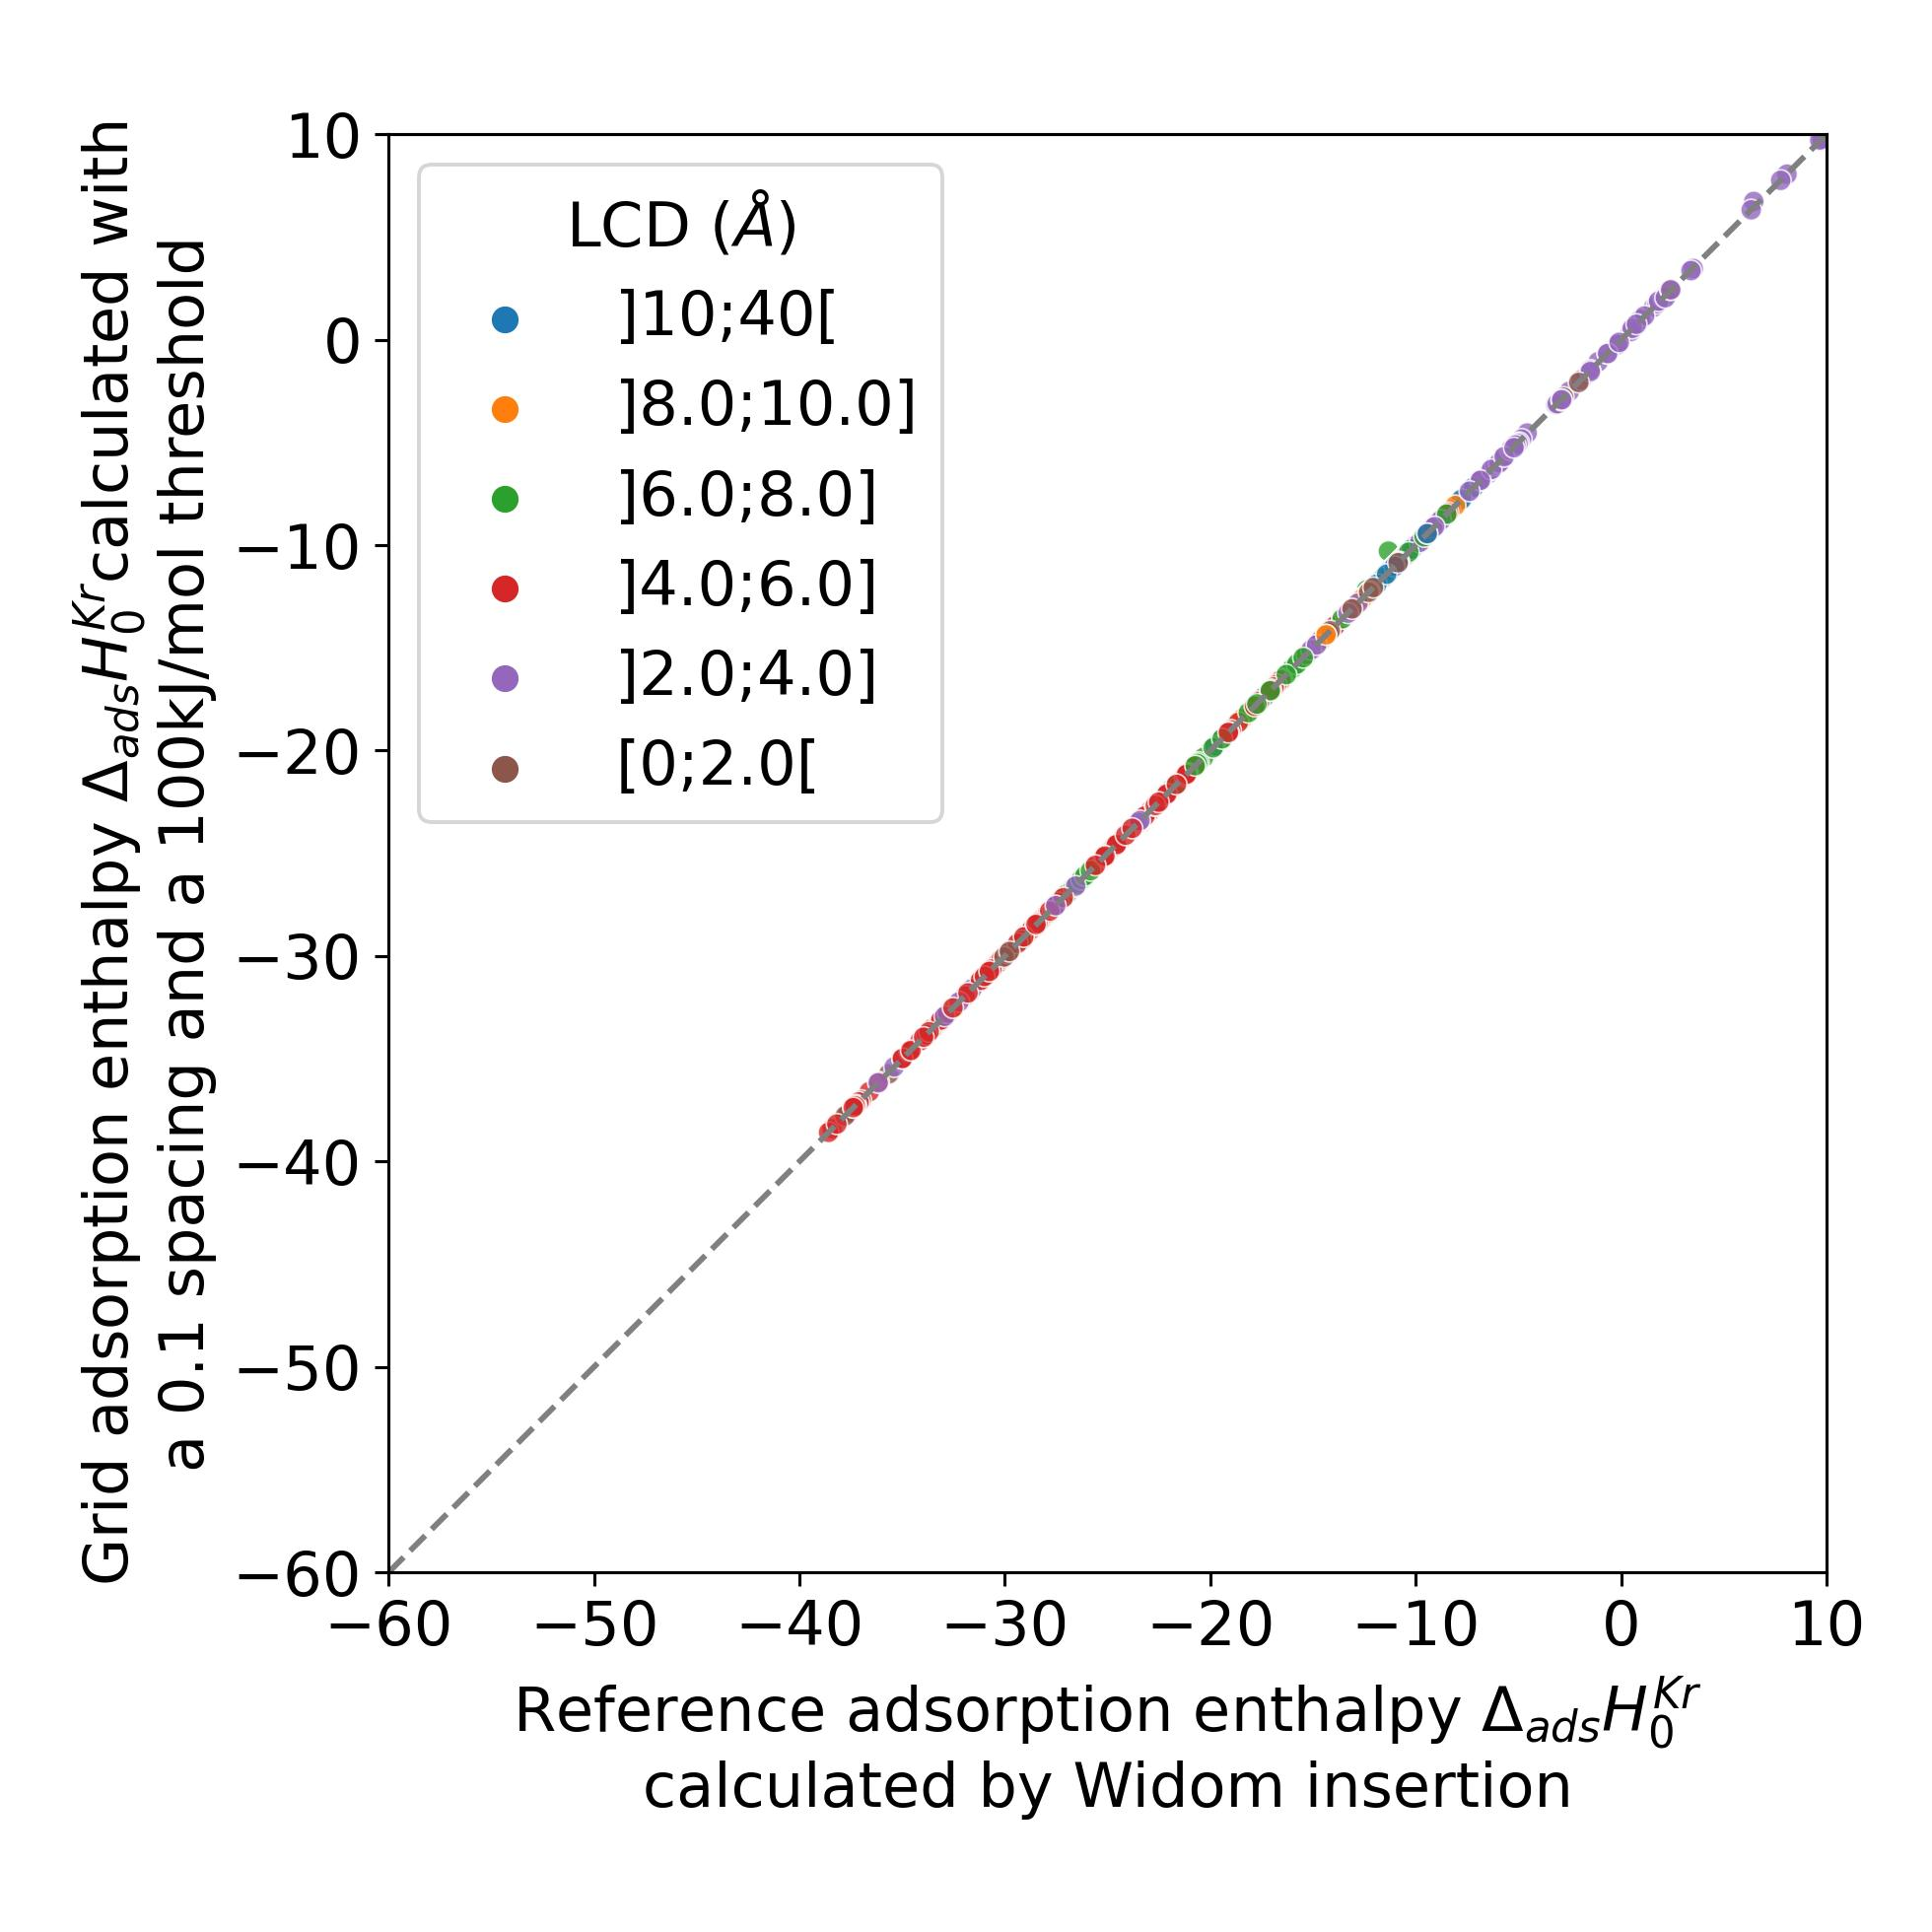
\includegraphics[width=0.45\textwidth]{figures/3-fastsim/H_Kr_0_widom_vs_H_Kr_grid_overview.jpg}
    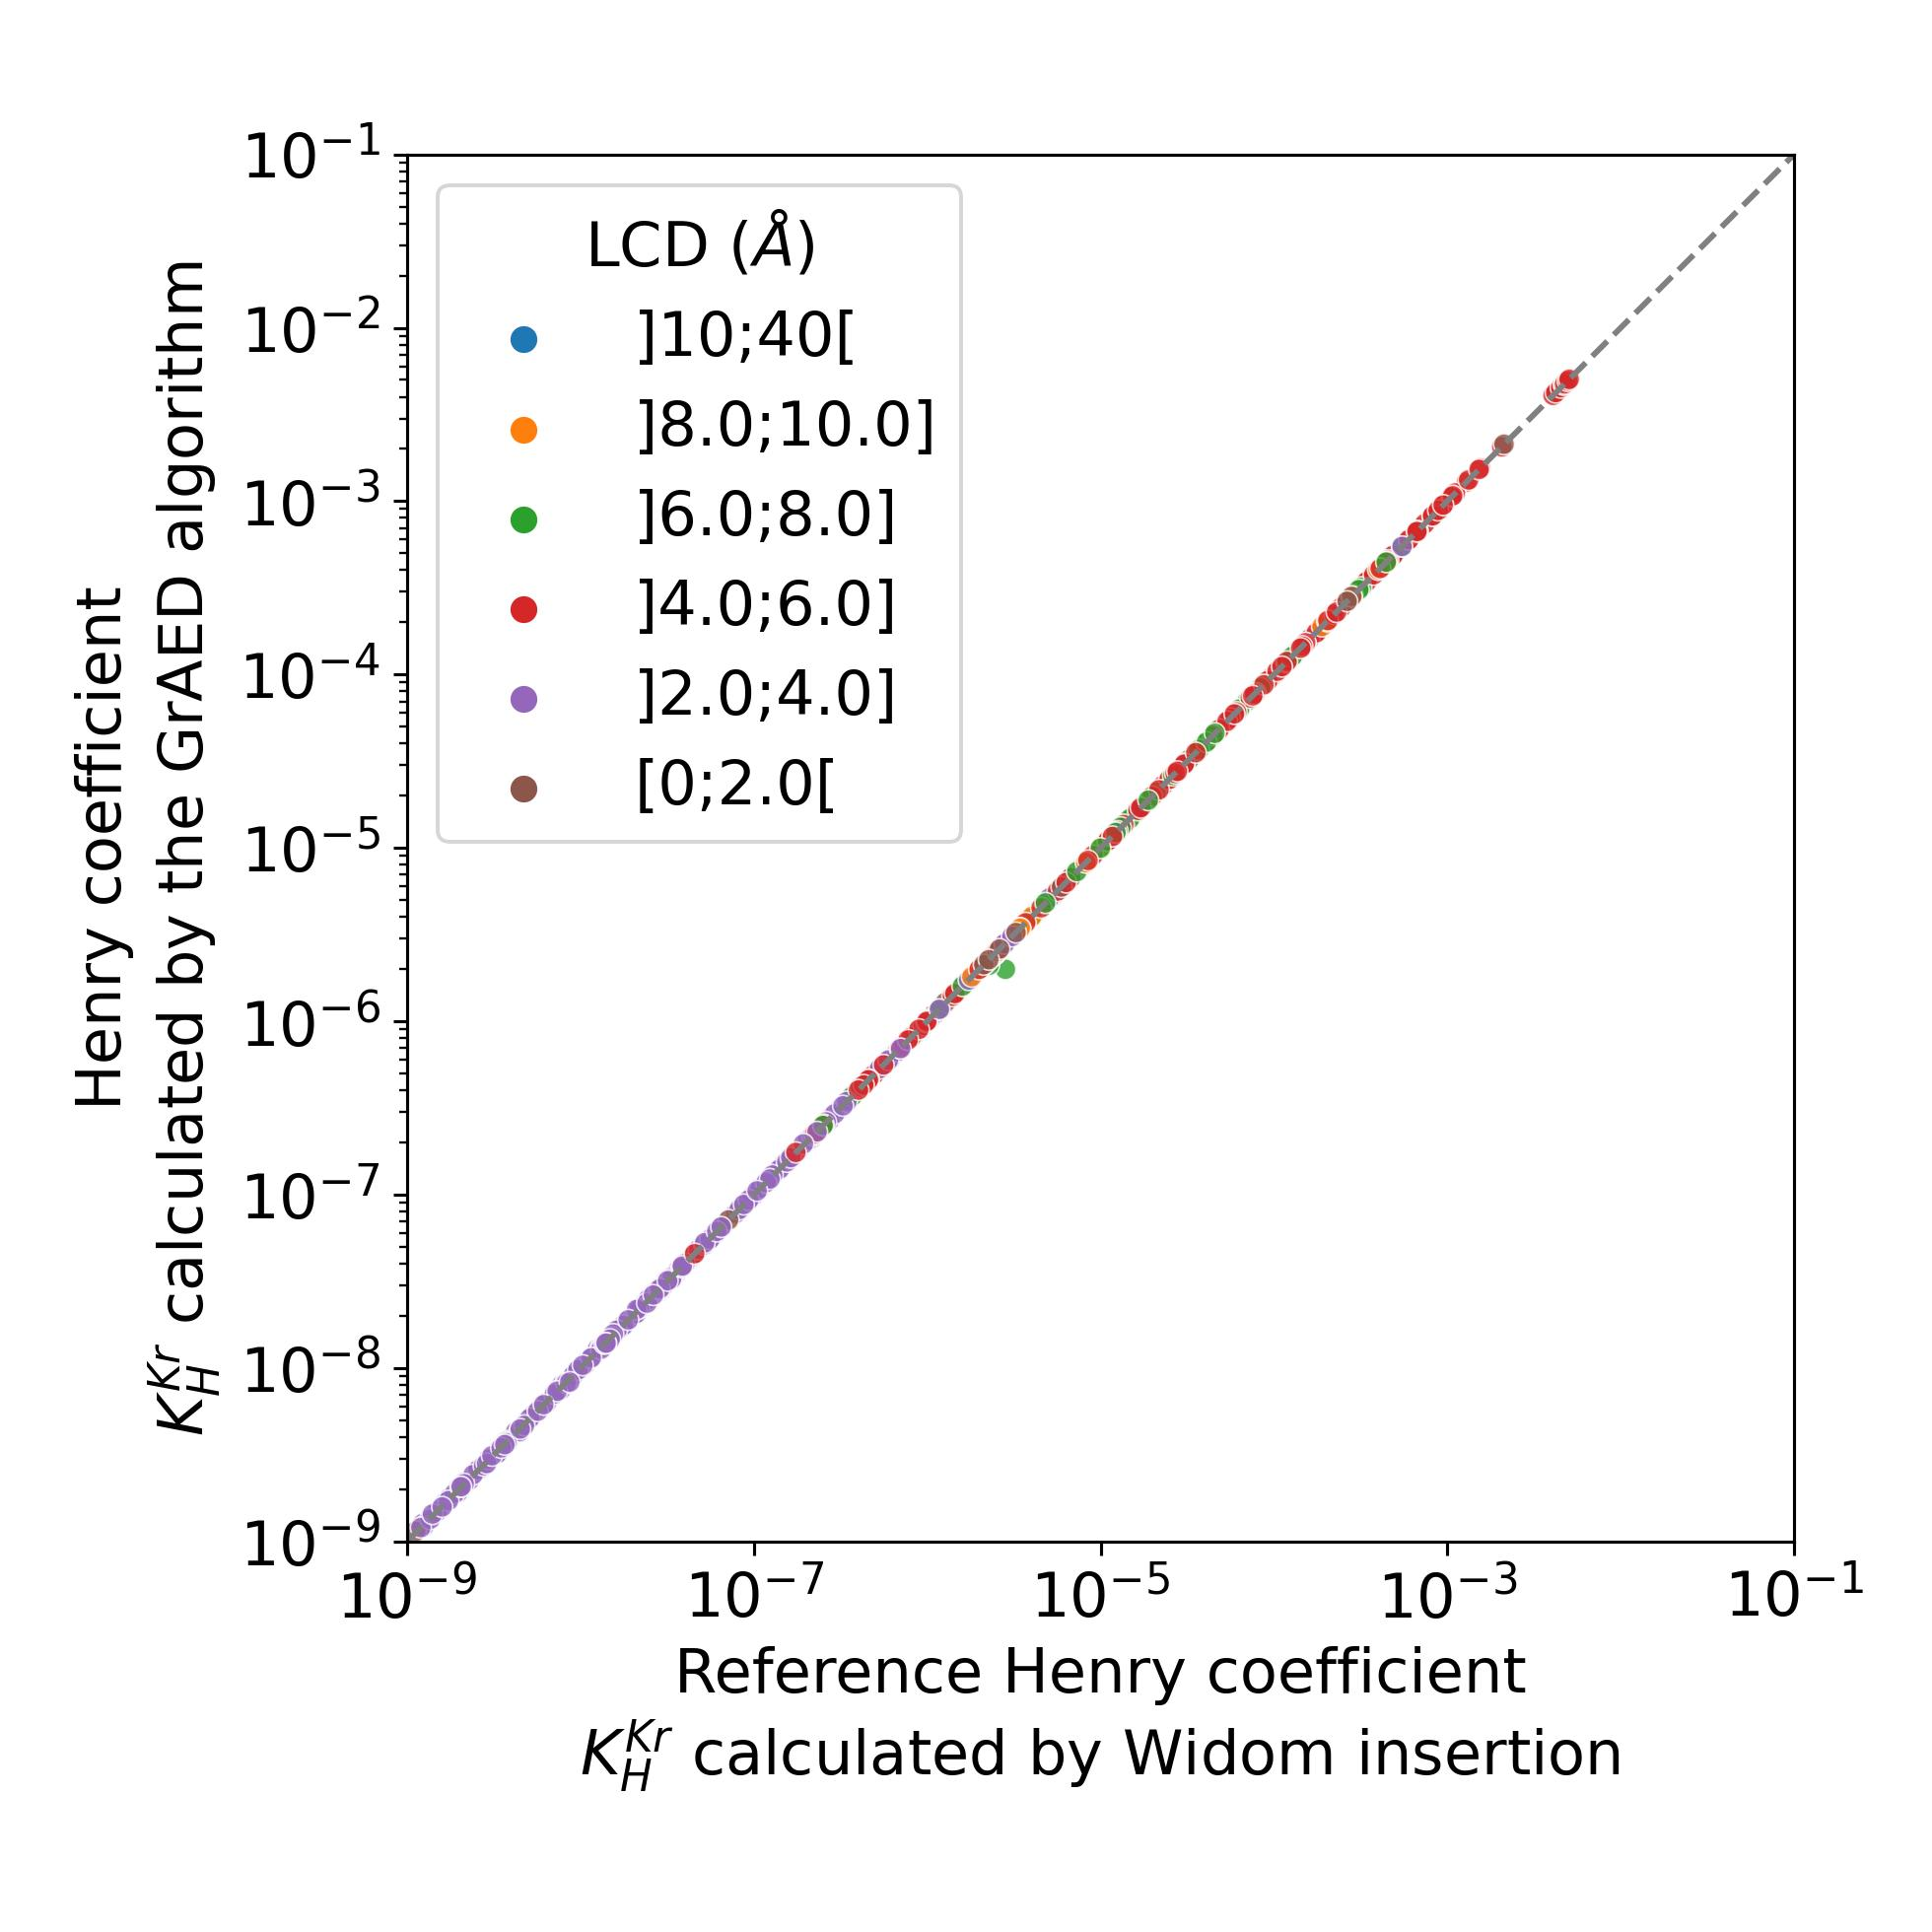
\includegraphics[width=0.45\textwidth]{figures/3-fastsim/K_Kr_widom_vs_K_Kr_grid_overview.jpg}
    \caption{Comparison of the krypton adsorption enthalpies (left) and the Henry constants (right) calculated by the optimized grid energy sampling (for a \SI{0.12}{\angstrom} spacing, a rejection parameter $\mu=0.8$ and an energy threshold $E\e{th}$ of \SI{100}{\kilo\joule\per\mole}) and by the Widom insertion of RASPA2 with 100,000 cycles. }\label{fgr:grid_widom_kr}
\end{figure}

First, the adsorption properties of krypton were also calculated using the same grid spacing of \SI{0.12}{\angstrom}. The accuracy achieved is approximately equivalent, with an RMSE and MAE on the krypton adsorption enthalpy of around \SI{0.02}{\kilo\joule\per\mole} and \SI{0.01}{\kilo\joule\per\mole}. As shown in Figure~\ref{fgr:grid_widom_kr}, there is a strong correlation observed for both the adsorption enthalpy (on a linear scale) and the Henry constant (on a logscale). The RMSE for the base 10 logarithm of the Henry constant (in \si{\milli\mole\per\gram\per\pascal}) is typically $0.002$, , which is similar to the accuracy obtained for xenon. The relative error in the adsorption enthalpies of xenon and krypton does not exceed {0.1\%} (values of the enthalpy have order of magnitude of dozens of \si{\kilo\joule\per\mole}), and thus, the error  in the xenon/krypton exchange enthalpy is expected to be very close to this value. Consequently, there is no significant impact on the exchange enthalpy. To evaluate the selectivity, it is necessary to consider the relative error in the adsorption free energy, which is a logarithmic transformation of the Henry constant. This relative error can be estimated to be around {0.2\%} (for a Henry constant of $10{-4}$~\si{\milli\mole\per\gram\per\pascal}), which is also approximately the expected relative error in the exchange Gibbs free energy or the logarithm of the selectivity.

\begin{figure}[ht]
  \centering
    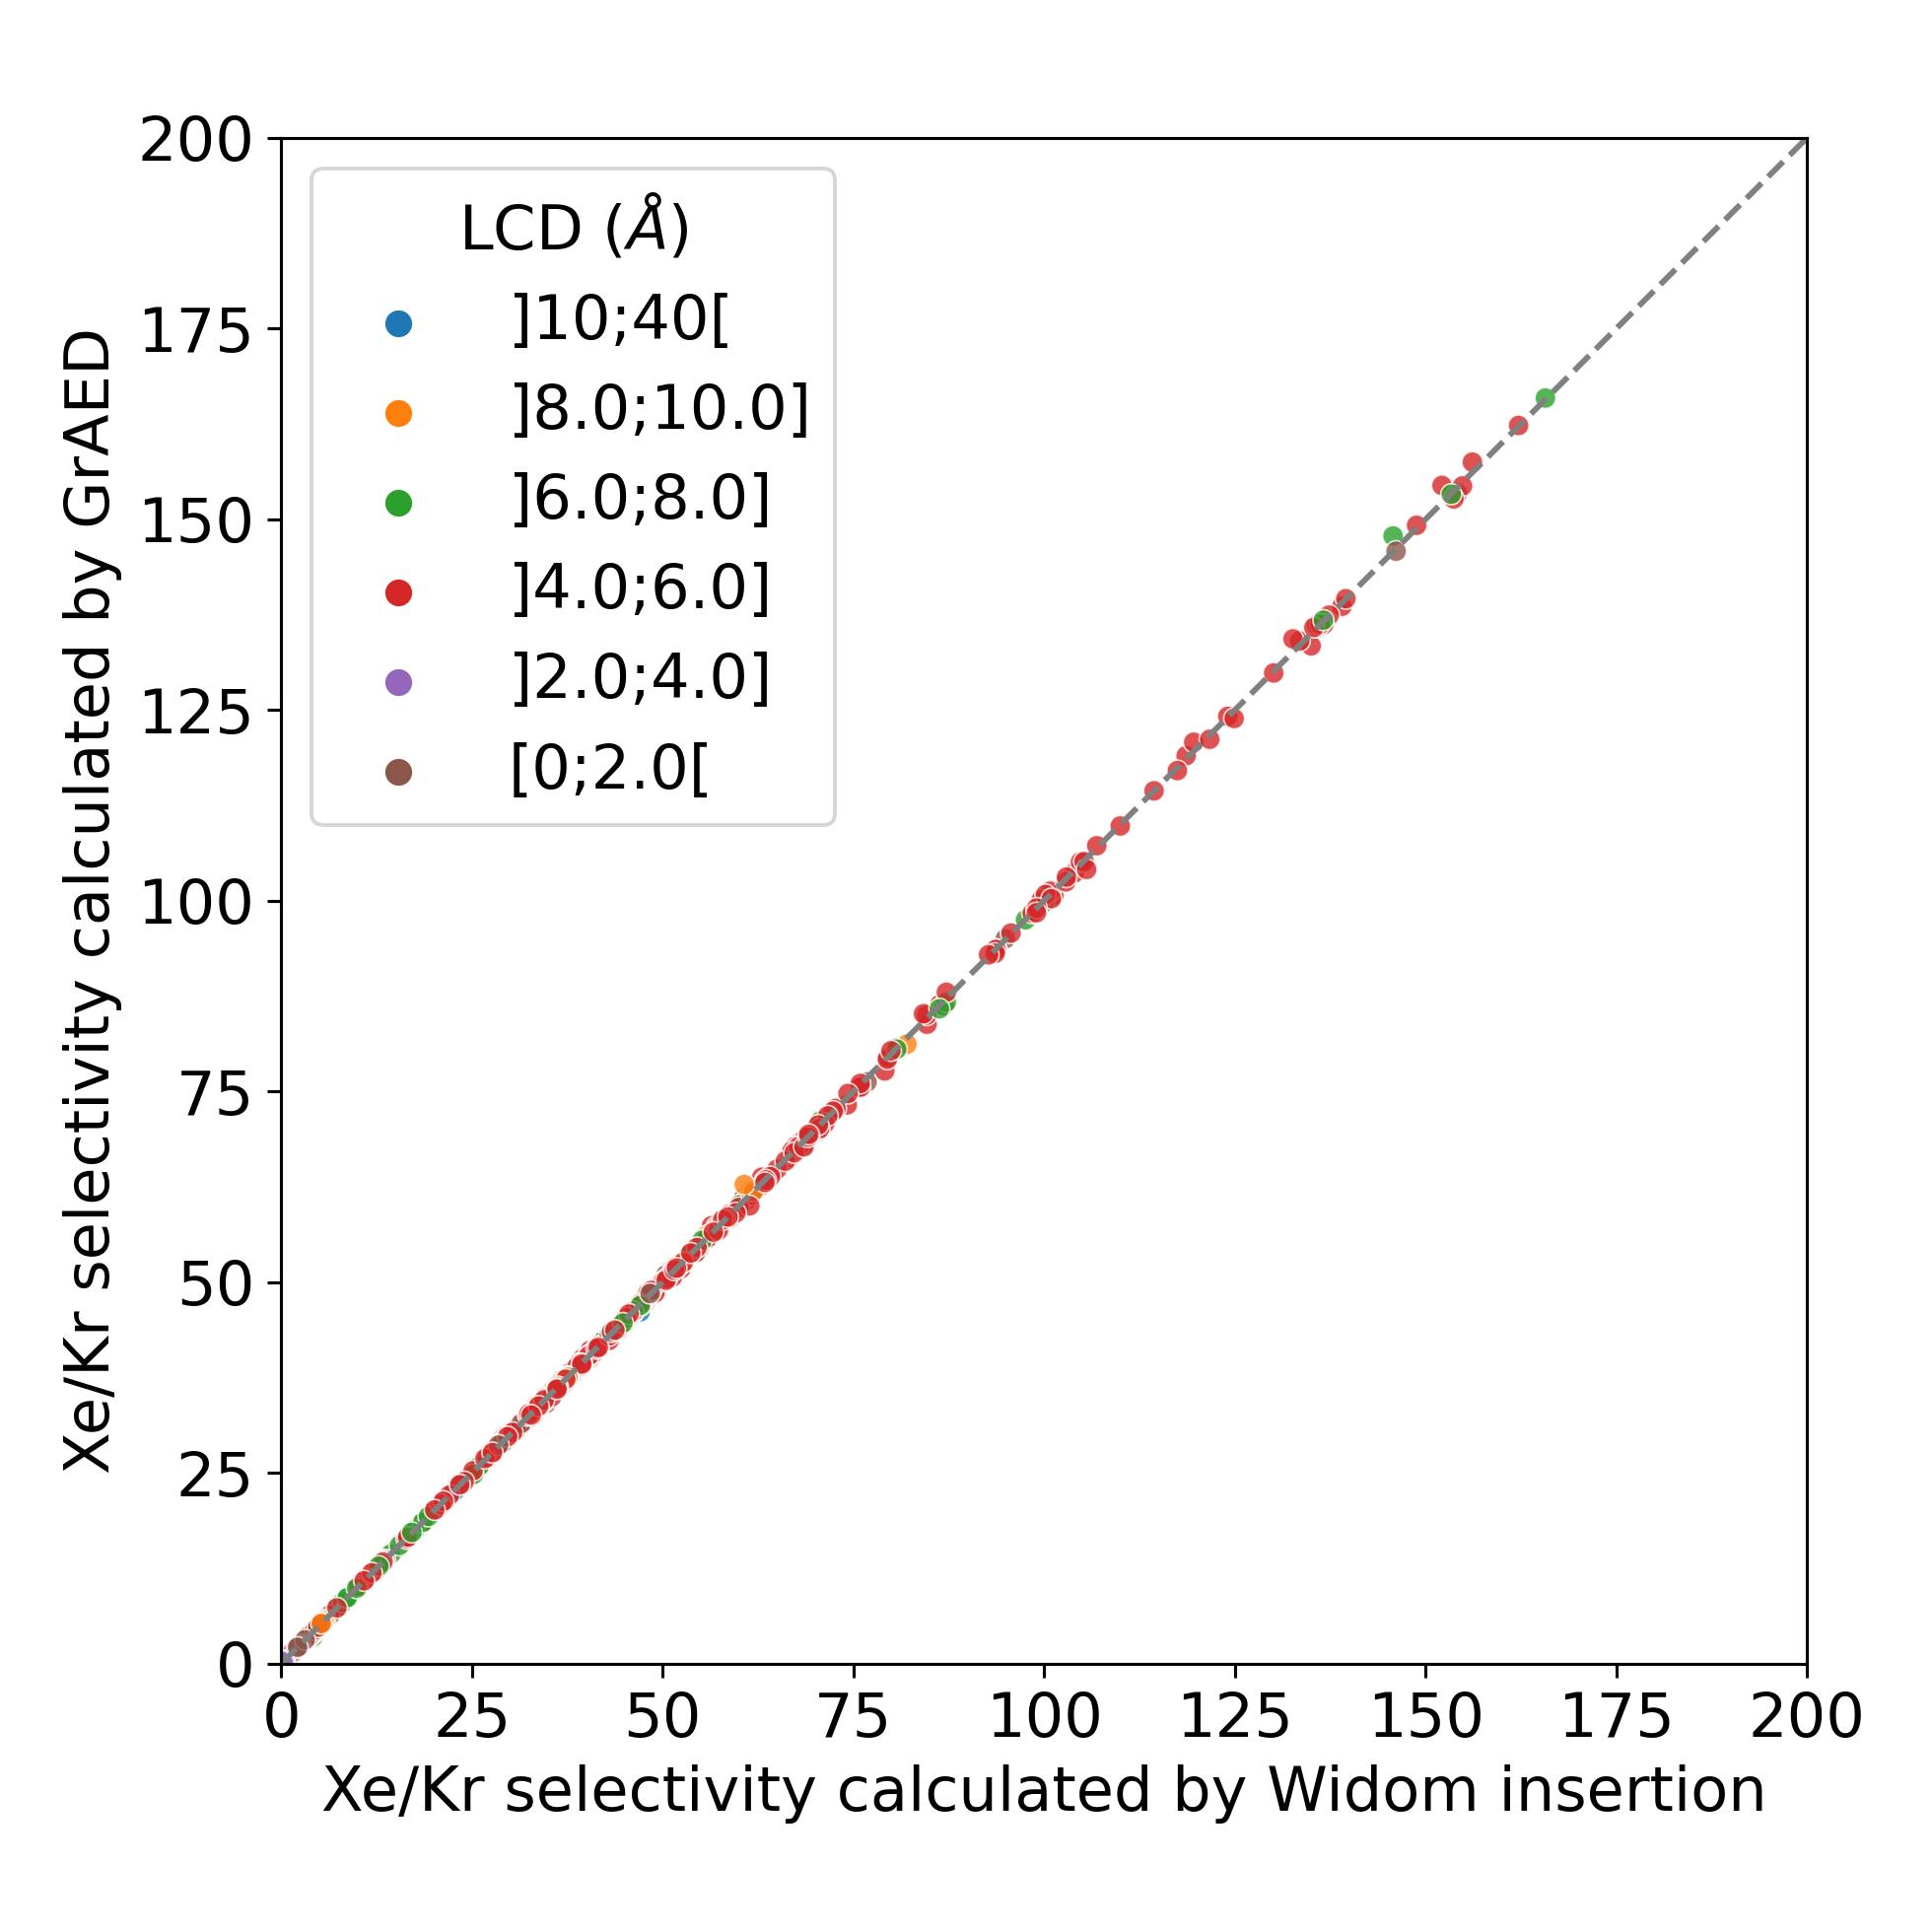
\includegraphics[width=0.45\textwidth]{figures/3-fastsim/s_0_widom_vs_s_0_grid_overview.jpg}
    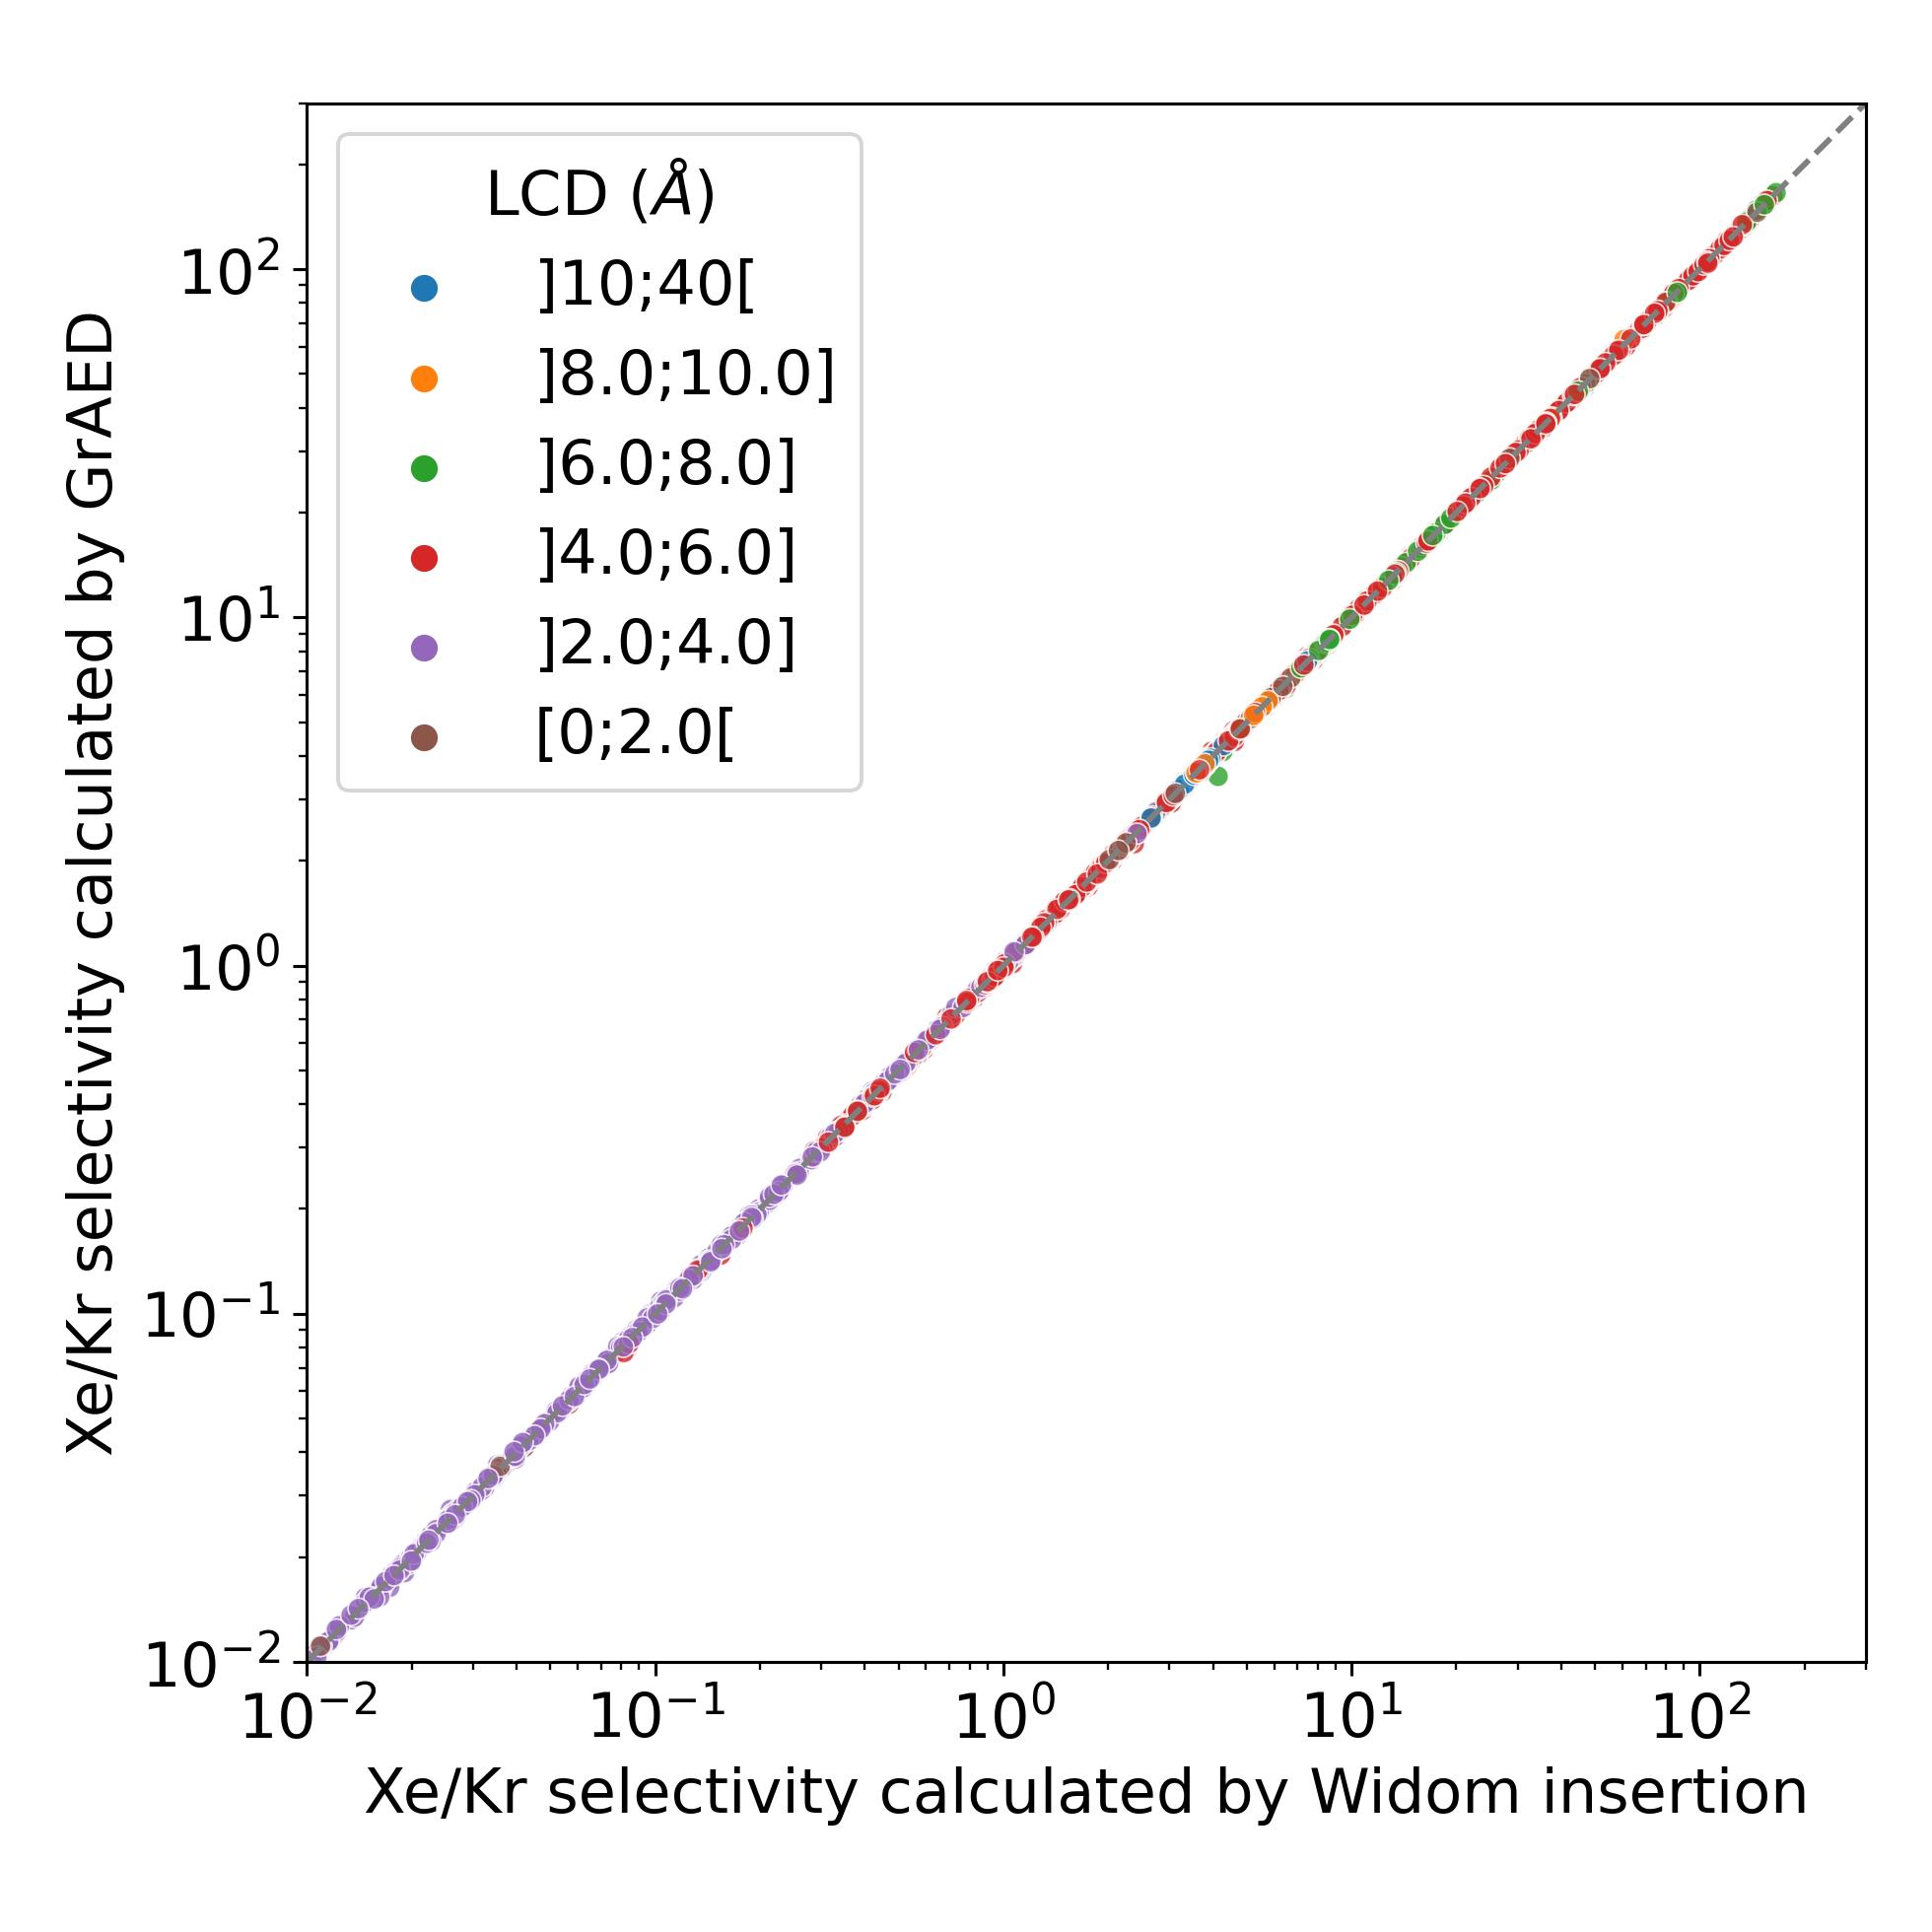
\includegraphics[width=0.45\textwidth]{figures/3-fastsim/s_0_widom_vs_s_0_grid_overview_log.jpg}
    \caption{Comparison of the Xe/Kr selectivity calculated by the optimized grid energy sampling (for a \SI{0.12}{\angstrom} spacing, a rejection parameter $\mu=0.8$ and an energy threshold $E\e{th}$ of \SI{100}{\kilo\joule\per\mole}) and by the Widom insertion of RASPA2 with 100,000 cycles. On the left, the axes are in linear scale, whereas the log scale has been used on the right. }\label{fgr:grid_widom_selectivity}
\end{figure}

Figure~\ref{fgr:grid_widom_selectivity} demonstrates that the selectivity is accurately represented by the new grid sampling, particularly when considering the logarithmic transformation. The RMSE and MAE for the selectivity values are approximately $0.097$ and $0.035$, respectively, which are quite low compared to the selectivity values of interest (above $10$). For these selective structures, the relative error is actually below {0.1\%}. For base 10 logarithm of the selectivity or the exchange Gibbs free energy, the RMSE is around $0.014$, indicating a precise understanding of the order of magnitude of the selectivity. If the selectivity were expressed in powers of ten, the exponent would be known with a precision of $\pm 0.014$.


The average computation time required to calculate the selectivity value for a structure in the CoRE MOF 2019 database is approximately \SI{6.5}{\second}, with the krypton component taking about \SI{3.5}{\second} to compute. If an algorithm computes both selectivity values simultaneously, it is possible to save the time required for initializing the software, which can marginally improve this overall time. This computation time is still much lower than the time required for two Widom insertions.

Having demonstrated the high accuracy and efficiency of the GrAED algorithm for evaluating selectivity at low pressures, the next step is to investigate relationships between descriptors obtained using the grid-based algorithm and the selectivity at ambient pressure.

\subsection{Description of the ambient-pressure selectivity}

Upon initial observation of the left plot in Figure~\ref{fgr:grid_ambient_selectivity}, the selectivity at ambient pressure shows no correlation with the selectivity at infinite dilution. This suggests that the sampling performed may be ineffective in determining the selectivity values at higher pressures. However, the right plot suggests the existence of a correlation between the logarithm of the selectivity values. The absence of correlation observed in the linear scale plot is actually a phenomenon specific to highly selective materials, which is discussed in detail in Chapter 2. This phenomenon corresponds to a selectivity decrease exhibited by certain highly selective materials (at infinite dilution). In simpler terms, the saturation of the most selective sites diminishes the selectivity of the remaining sites for xenon/krypton separation in these materials.

\begin{figure}[ht]
  \centering
    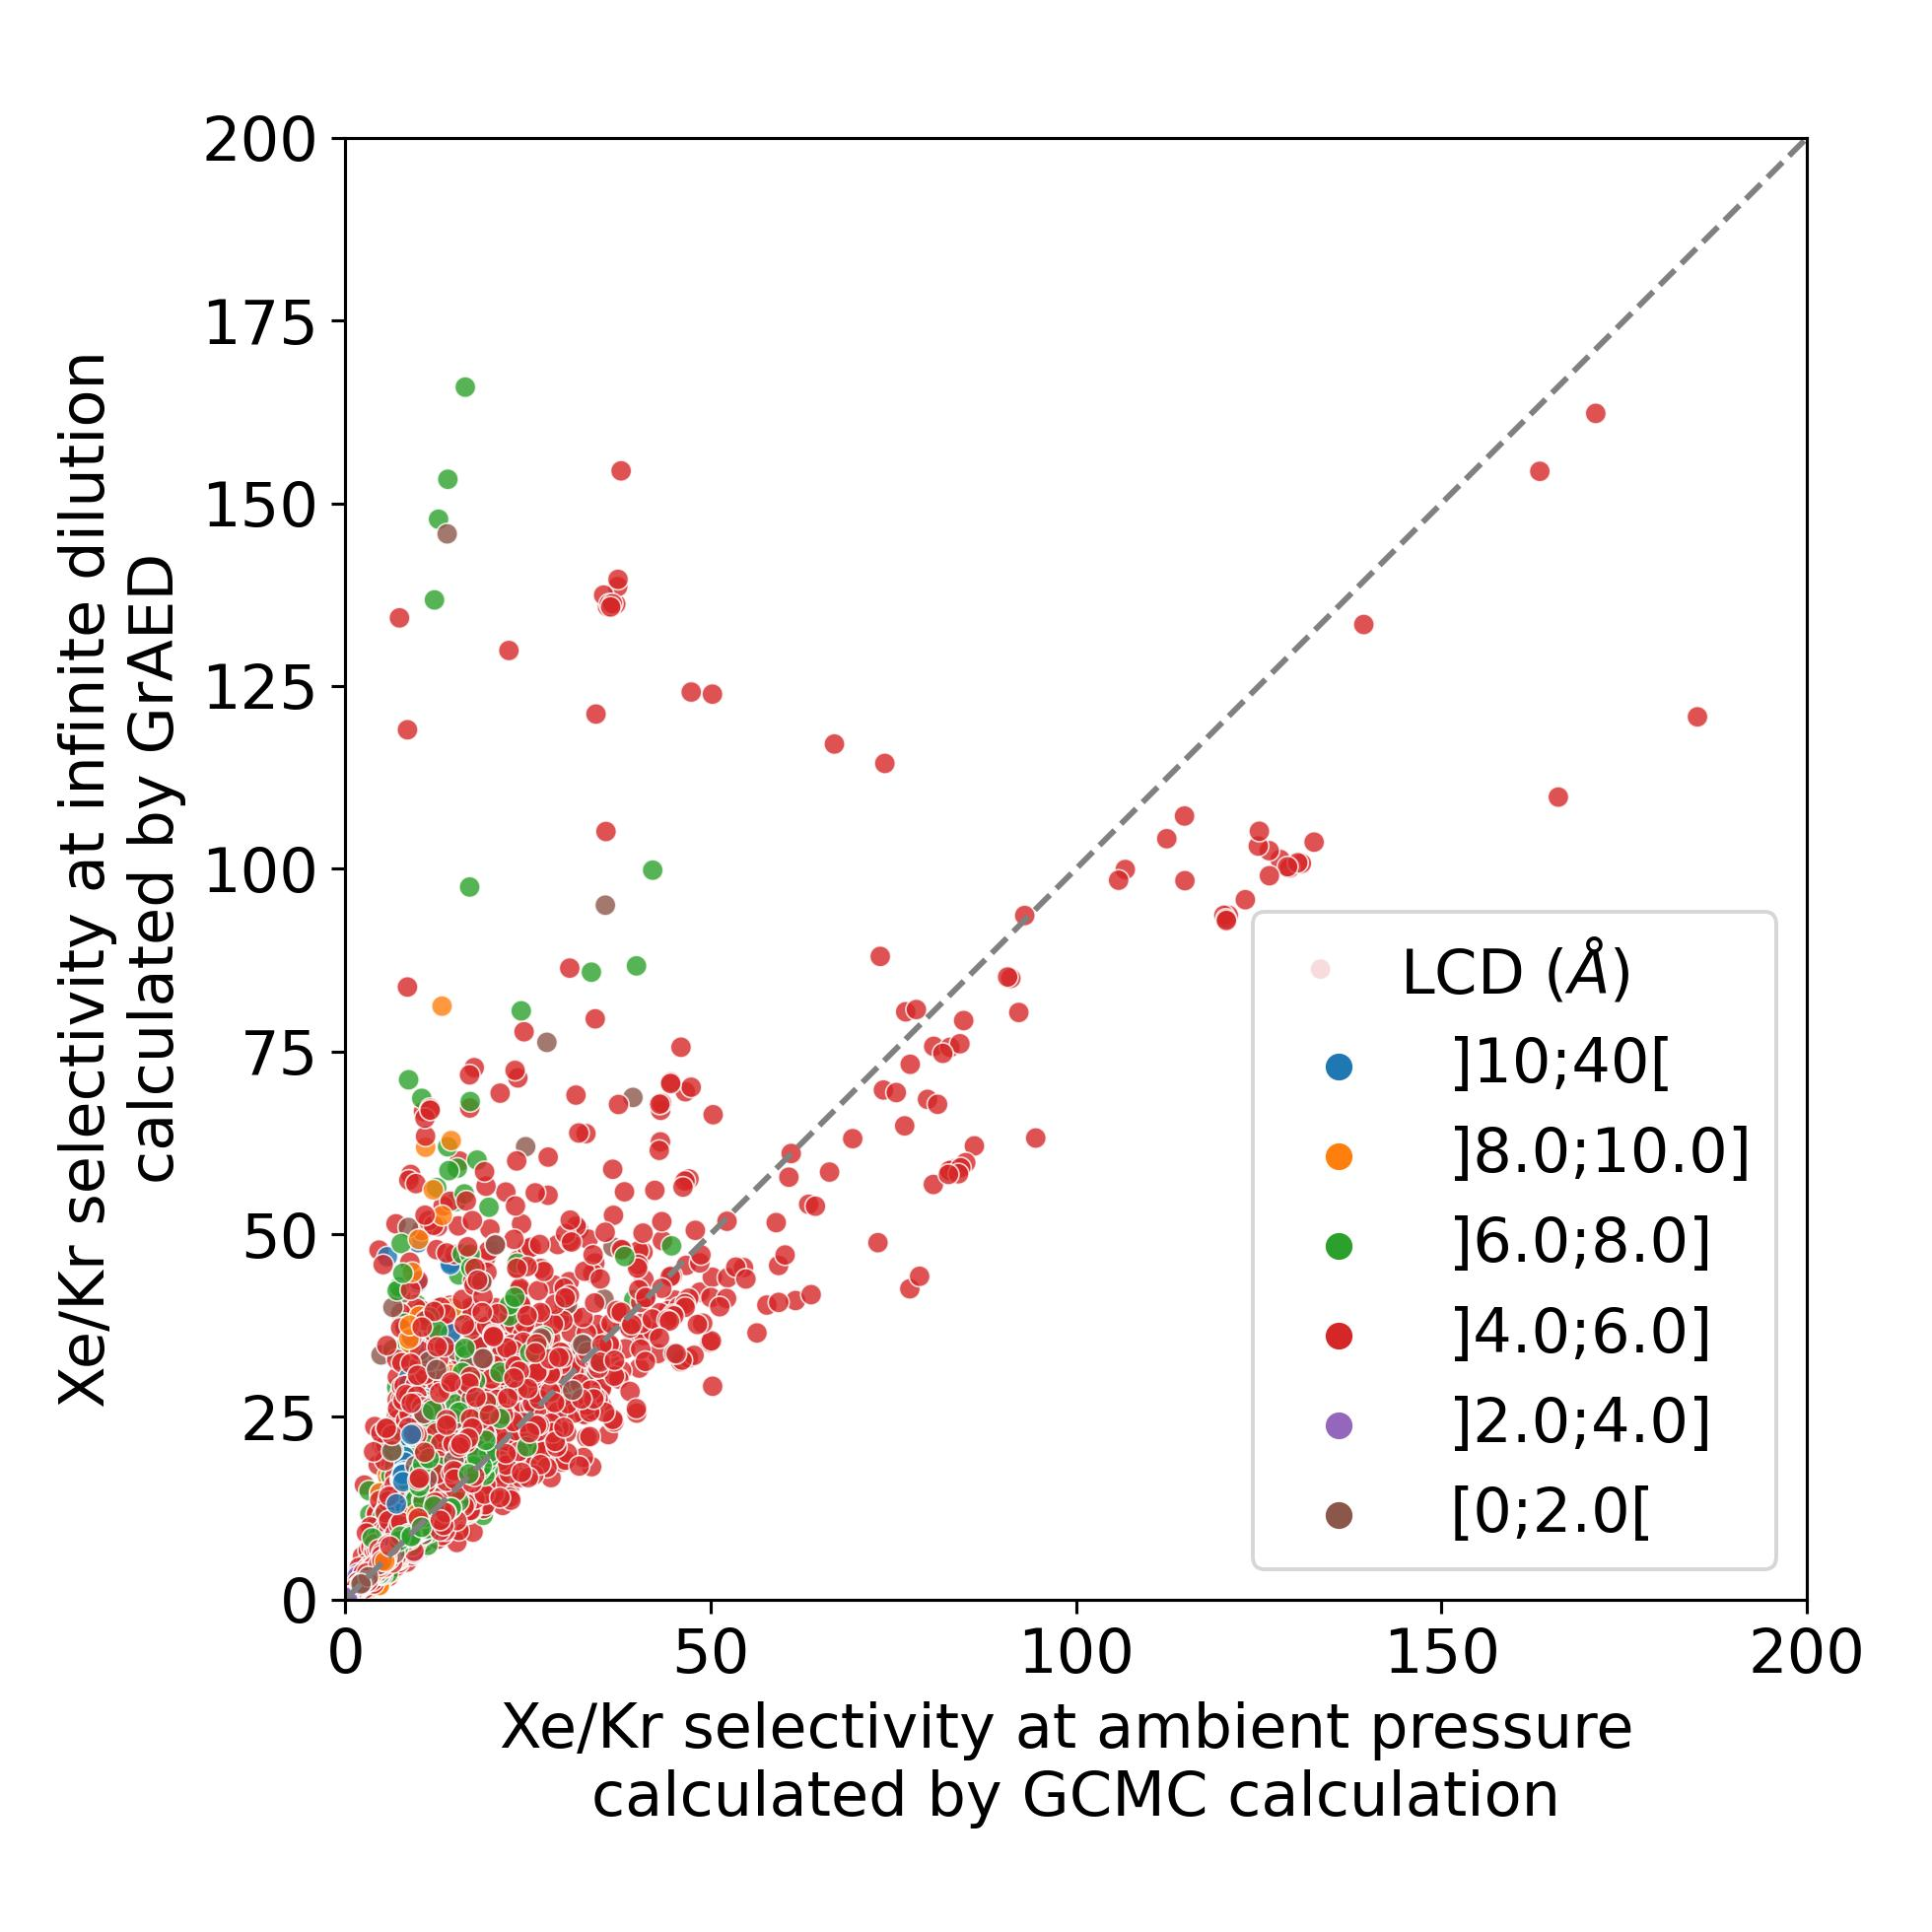
\includegraphics[width=0.45\textwidth]{figures/3-fastsim/s_2080_vs_s_0_grid_overview.jpg}
    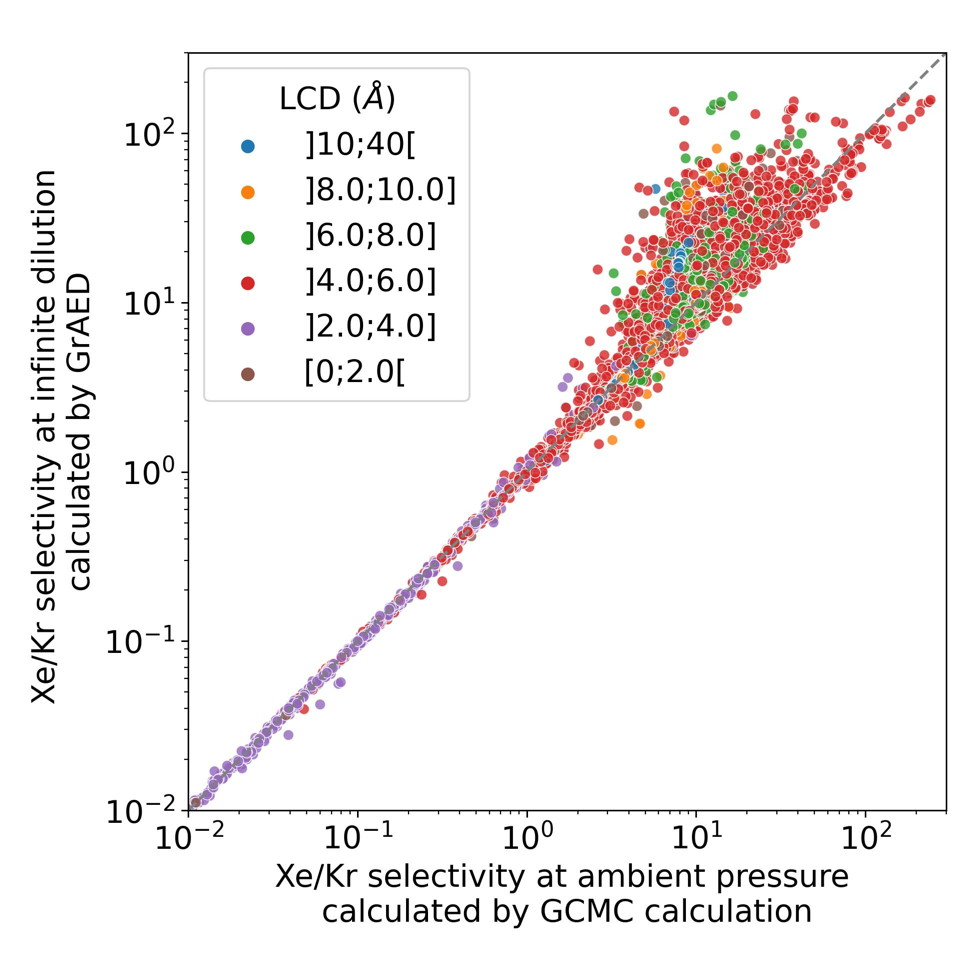
\includegraphics[width=0.45\textwidth]{figures/3-fastsim/s_2080_vs_s_0_grid_overview_log.jpg}
    \caption{Comparison of the low-pressure Xe/Kr selectivity calculated by the GrAED algorithm (same parameters) and the ambient-pressure selectivity calculated by GCMC simulations of RASPA2 with 100,000 cycles. On the left, the axes are in linear scale, whereas the log scale has been used on the right. }\label{fgr:grid_ambient_selectivity}
\end{figure}

The aim is to design descriptors that can help distinguish materials exhibiting a drop in selectivity at higher pressure from those maintaining high selectivity at higher pressure. Three concepts are proposed to gain a better understanding of the origin of this selectivity drop: (1) other adsorption thermodynamic quantities, (2) higher temperature averaging can also be a good proxy to understand higher pressure adsorption, and (3) statistical quantities derived from the energy distributions. All of these descriptors can be obtained through a grid sampling; however, it is important to note that this method cannot capture guest-guest interactions occurring at higher pressures.


\subsubsection{Thermodynamic quantities}

In the previous chapter, various thermodynamic quantities were calculated at infinite dilution, including adsorption and exchange Gibbs free energies, enthalpies, and entropies. For the separation of xenon and krypton, a total of nine different descriptors can be generated. The relationship between these quantities and the selectivity values at high pressure will be examined. In the introduction, the relationship between the exchange Gibbs free energy and the selectivity at infinite dilution was already discussed, as shown in Figure~\ref{fgr:grid_ambient_selectivity} that plotted the logarithmic transform of the infinite dilution selectivity. This descriptor holds significant importance as it establishes an initial reference value for understanding the problem. The selectivity at high pressure can be viewed as the selectivity at infinite dilution with an additional shift, accounting for the specific adsorption behavior at higher pressures in a given material.


\begin{figure}[ht]
  \centering
    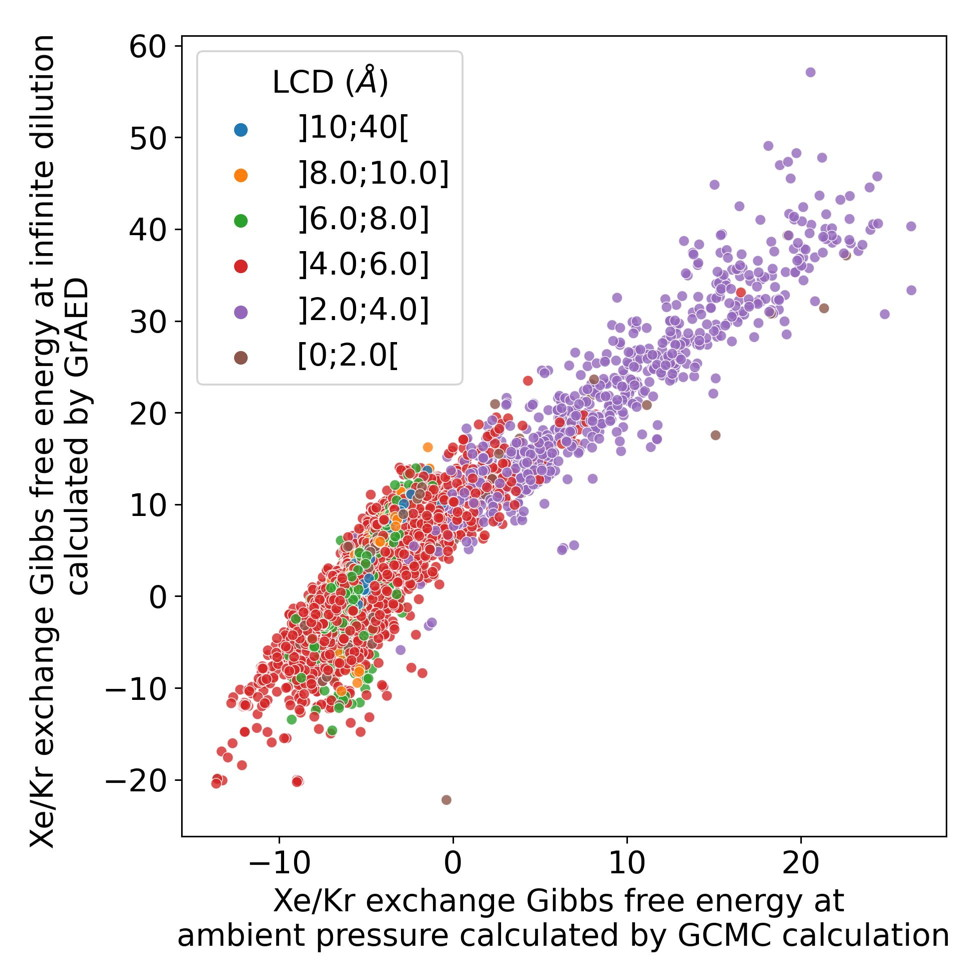
\includegraphics[width=0.45\textwidth]{figures/3-fastsim/G_2080_vs_G_Xe_grid_overview.jpg}
    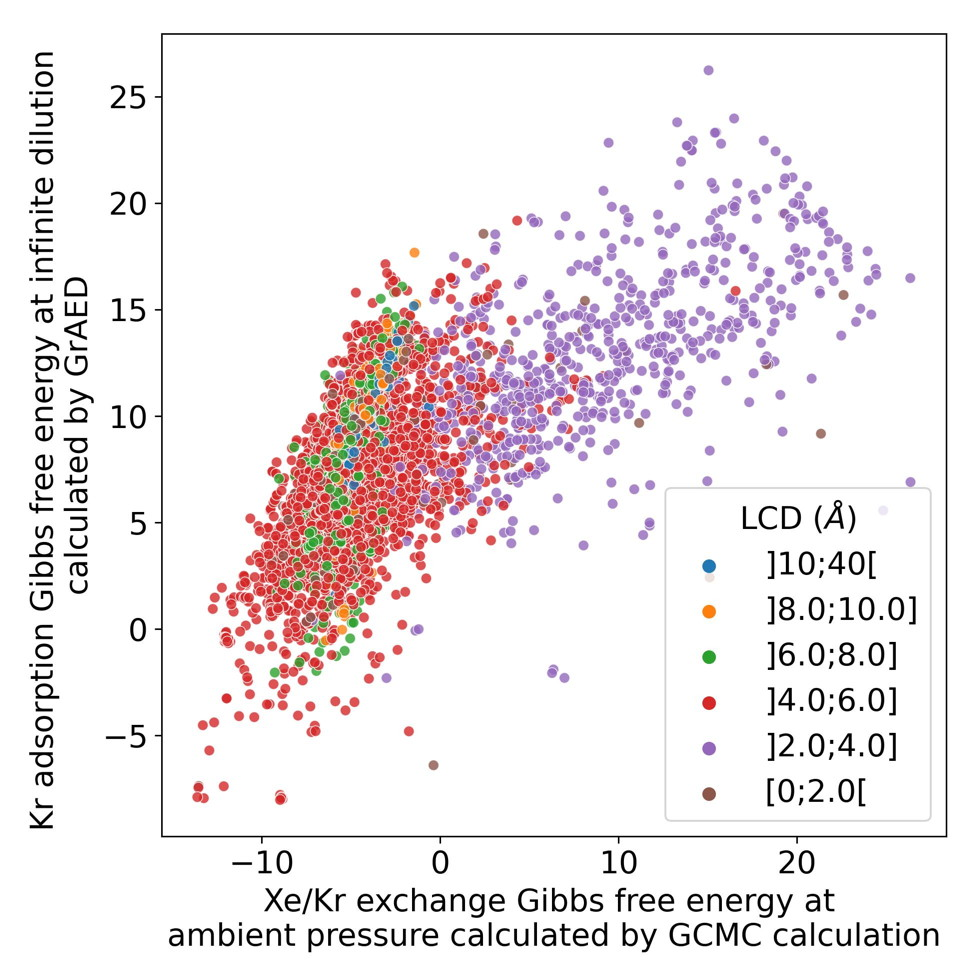
\includegraphics[width=0.45\textwidth]{figures/3-fastsim/G_2080_vs_G_Kr_grid_overview.jpg}
    \caption{Comparison of the ambient-pressure Xe/Kr exchange Gibbs free energy calculated by GCMC simulations of RASPA2 with 100,000 cycles and the low-pressure adsorption free energies of xenon (left) and krypton (right) in \si{\kilo\joule\per\mole} calculated by the GrAED algorithm (same parameters).}\label{fgr:grid_comp_gibbs}
\end{figure}

It comes as no surprise that a good adsorption of xenon is a good indication for the efficiency of the separation from krypton, as shown in Figure\ref{fgr:grid_comp_gibbs}, since there is a very strong correlation between the Xe/Kr exchange Gibbs free energy and the xenon adsorption Gibbs free energy. A very weak but positive correlation with the xenon adsorption Gibbs free energy is observed, indicating that a material suitable for efficient Xe/Kr separation would not exhibit very poor krypton adsorption, but rather an average performance. In other words, it is not possible to find a material that is highly effective for xenon adsorption and highly ineffective for krypton adsorption, which explains the theoretical limitation on selectivity, capped under $200$ (in our level of theory for CoRE MOF 2019 materials, see Figure~\ref{fgr:grid_widom_selectivity} and~\ref{fgr:grid_ambient_selectivity}) Experimentally, no material has achieved a selectivity value exceeding $100$.

\begin{figure}[ht]
  \centering
    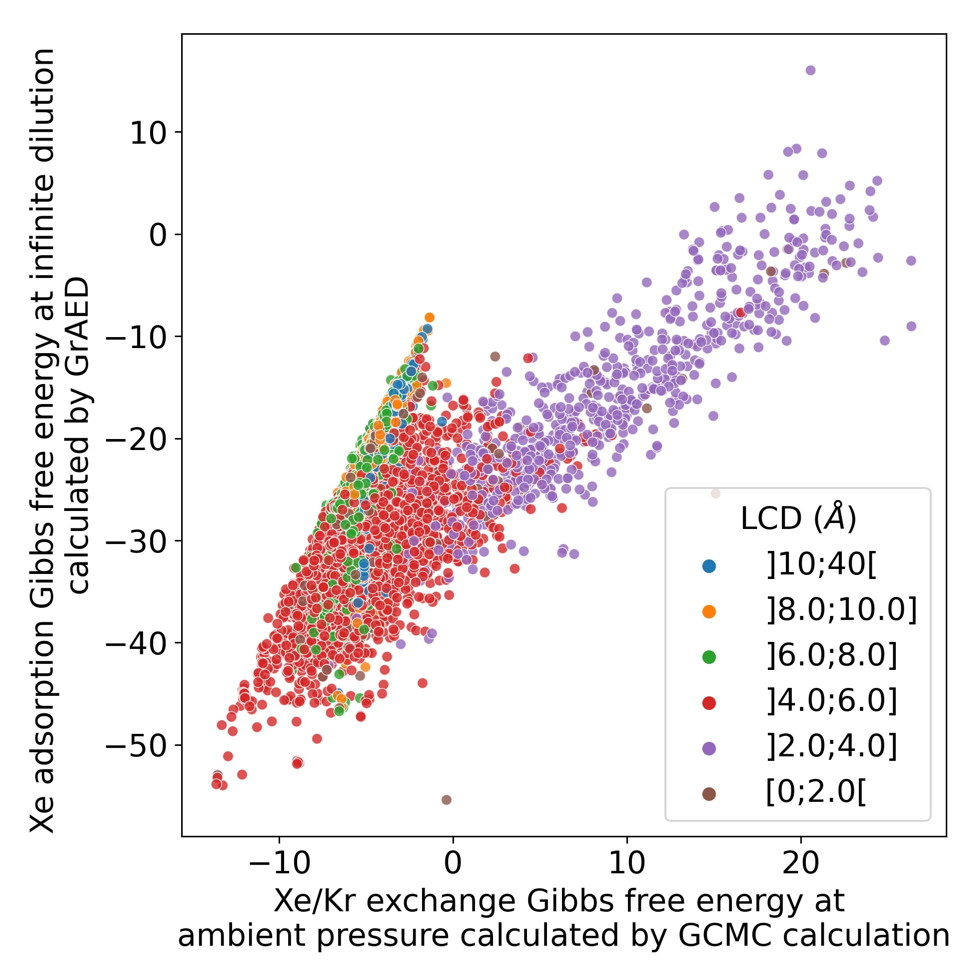
\includegraphics[width=0.45\textwidth]{figures/3-fastsim/G_2080_vs_H_Xe_grid_overview.jpg}
    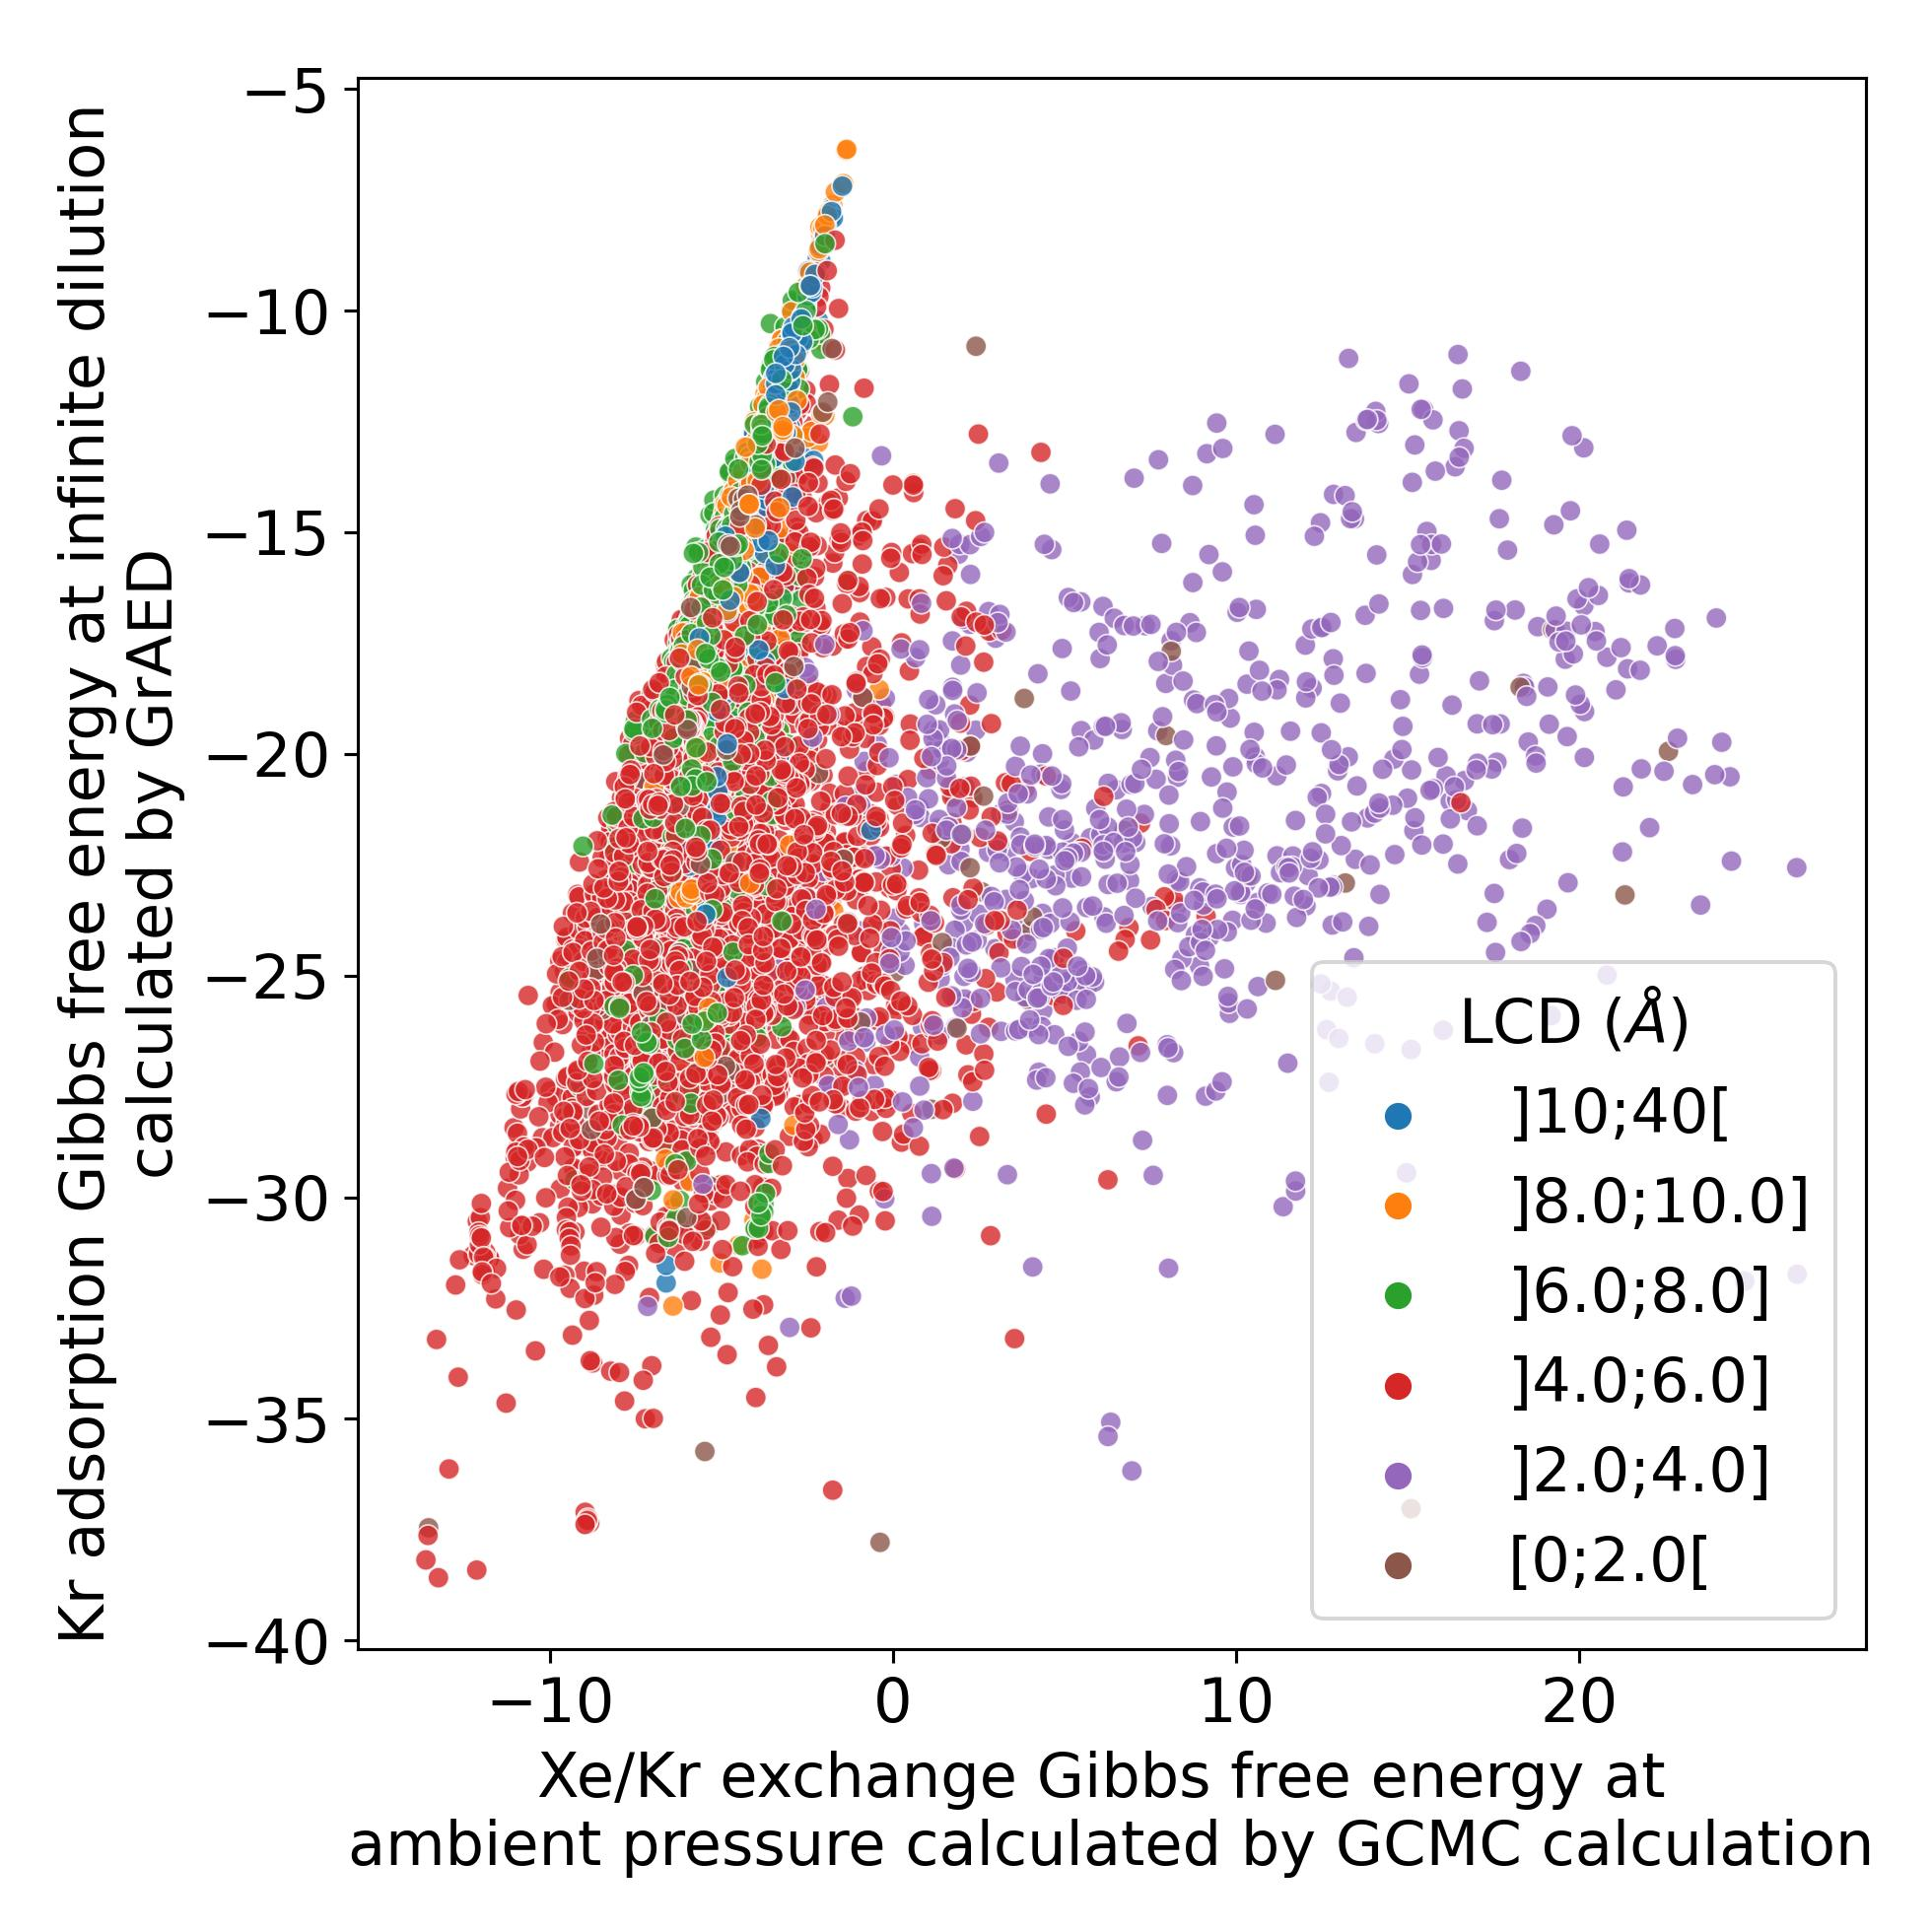
\includegraphics[width=0.45\textwidth]{figures/3-fastsim/G_2080_vs_H_Kr_grid_overview.jpg}
    \caption{Comparison of the ambient-pressure Xe/Kr exchange Gibbs free energy calculated by GCMC simulations of RASPA2 with 100,000 cycles and the low-pressure adsorption enthalpies of xenon (left) and krypton (right) in \si{\kilo\joule\per\mole} calculated by the GrAED algorithm (same parameters).}\label{fgr:grid_comp_enthalpy}
\end{figure}

The statement on the importance of xenon's adsorption attractiveness holds true when examining the adsorption enthalpies, as depicted in Figure~\ref{fgr:grid_comp_enthalpy}. A strong correlation is observed for the most selective materials. However, for less selective materials, xenon's adsorption enthalpy is insufficient for predicting the exchange Gibbs free energy at ambient pressure. A natural solution would be to include the performance of krypton adsorption. The difference between the two adsorption enthalpies yields the xenon/krypton exchange enthalpy, which serves as a metric for evaluating the separation process. Comparing it solely to krypton's adsorption enthalpy is also inadequate, as the very weak correlation suggests that it is not the main explanatory factor in the separation process.

\begin{figure}[ht]
  \centering
    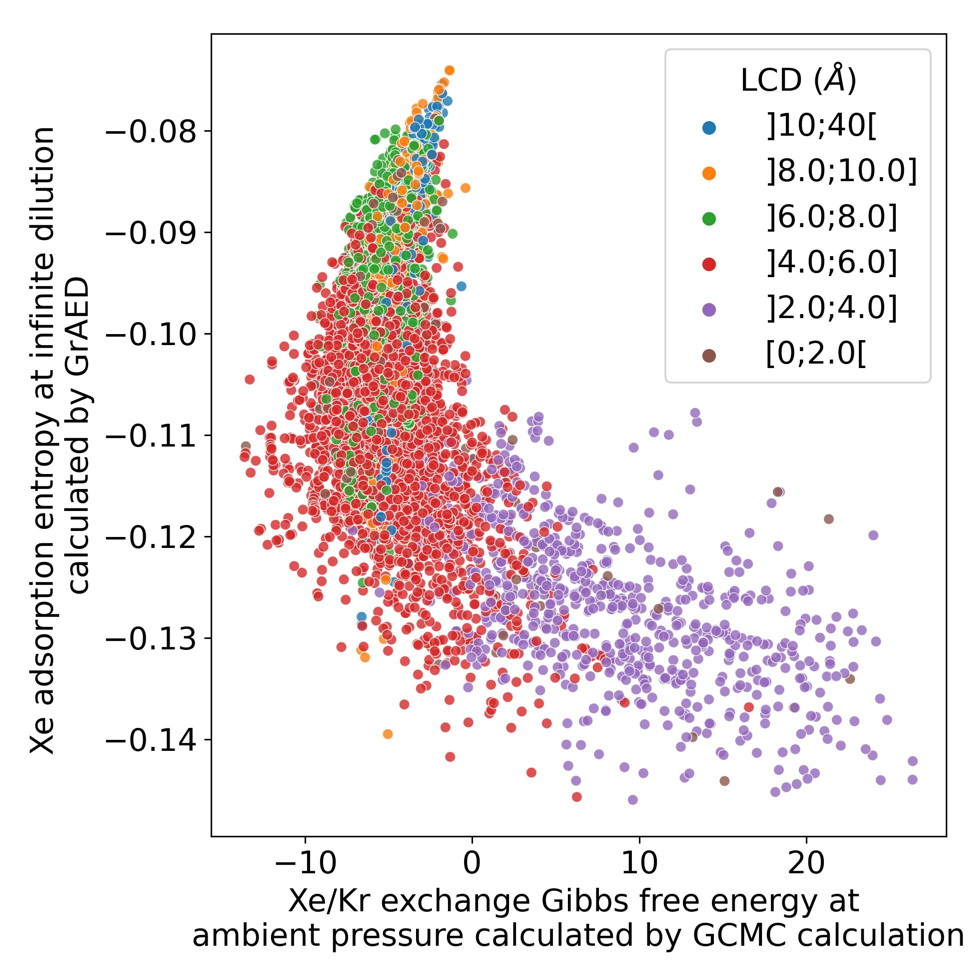
\includegraphics[width=0.45\textwidth]{figures/3-fastsim/G_2080_vs_S_Xe_grid_overview.jpg}
    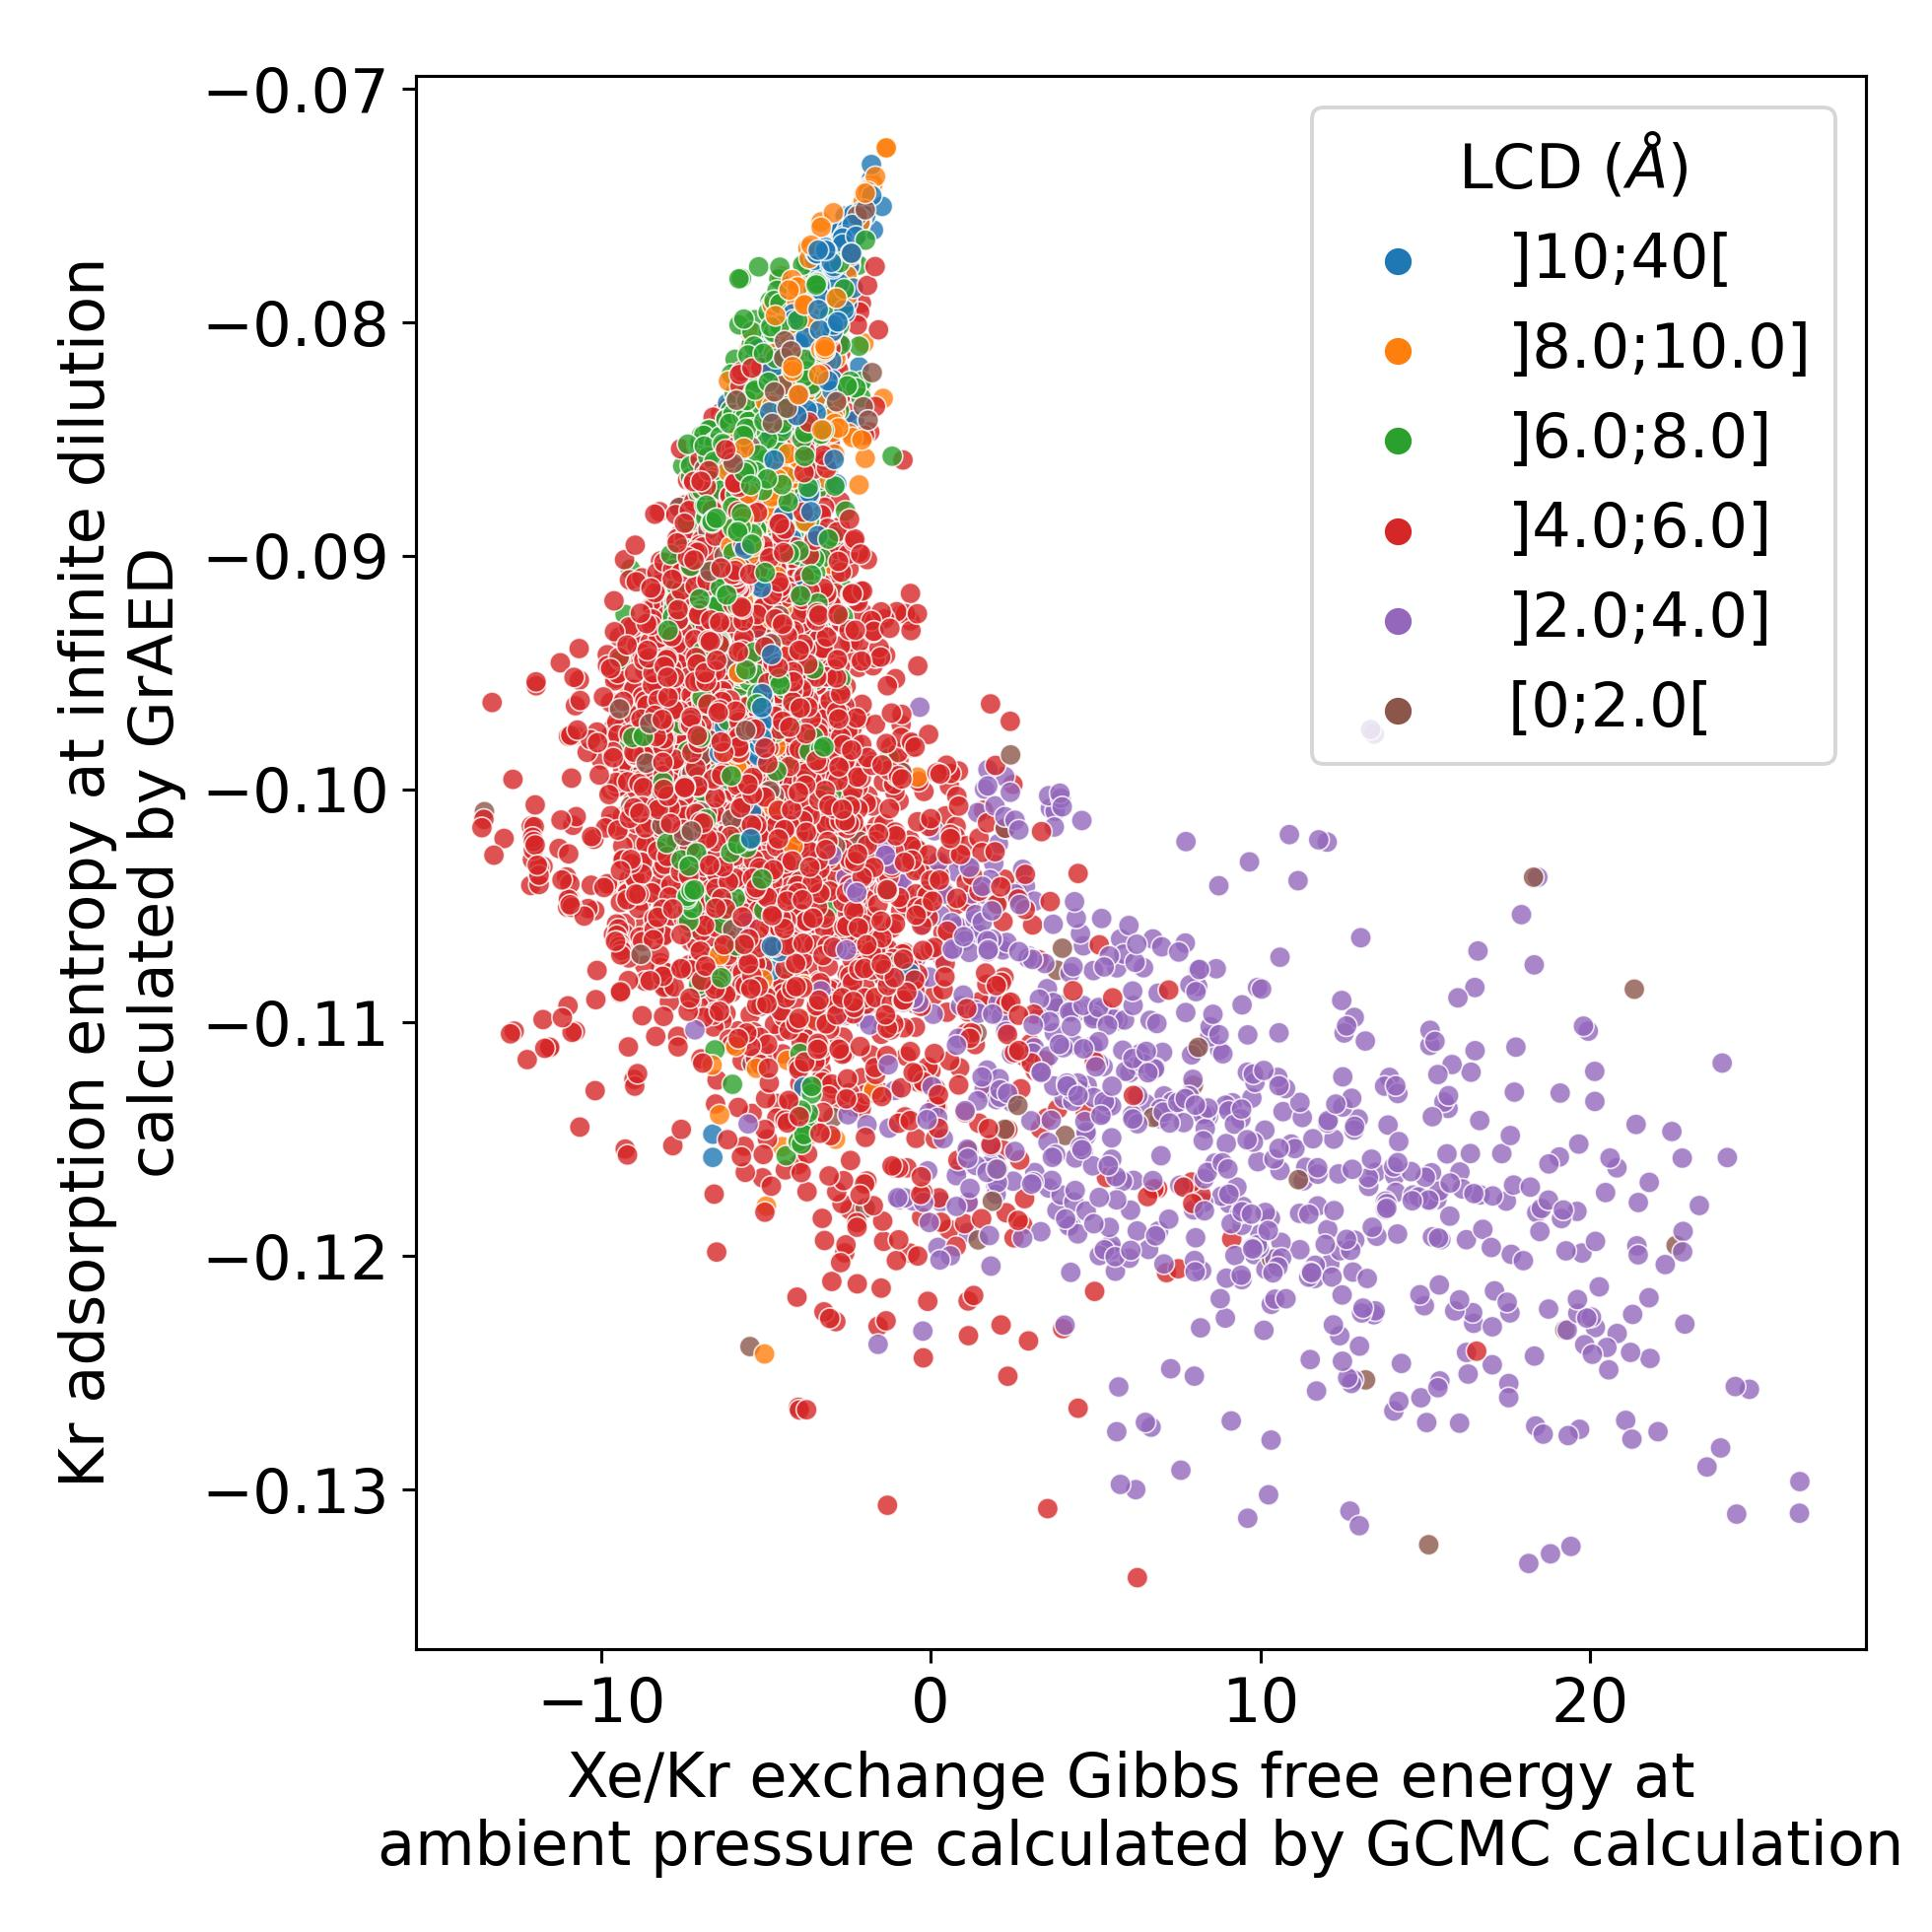
\includegraphics[width=0.45\textwidth]{figures/3-fastsim/G_2080_vs_S_Kr_grid_overview.jpg}
    \caption{Comparison of the ambient-pressure Xe/Kr exchange Gibbs free energy calculated by GCMC simulations of RASPA2 with 100,000 cycles and the low-pressure adsorption entropies of xenon (left) and krypton (right) in \si{\kilo\joule\per\mole\per\kelvin} calculated by the GrAED algorithm (same parameters).}\label{fgr:grid_comp_entropy}
\end{figure}

The correlation between the adsorption free energy of xenon and the Xe/Kr exchange free energy at ambient pressure, as well as the weak correlation with xenon's adsorption enthalpy, can be explained by the entropy values. The entropic term ($G=H-TS$), which represents the difference between enthalpy and free energy, has a minor influence on the correlation, as shown in Figure~\ref{fgr:grid_comp_entropy}. The values of the entropy are relatively stable (ranging from $-0.15$ to $-0.11$~\si{\kilo\joule\per\mole\per\kelvin}). However, for some structures with ambient-pressure exchange free energy between $-10$ and $0$~\si{\kilo\joule\per\mole}, there is a variation in entropy values ranging from $-0.11$ to $-0.07$~\si{\kilo\joule\per\mole\per\kelvin} despite having very similar enthalpy values. This discrepancy results in a difference between Gibbs free energy and enthalpy, with a potential span of $12$~\si{\kilo\joule\per\mole}, which explains the points deviating from the diagonal in the left plot of Figure~\ref{fgr:grid_comp_enthalpy}.

\begin{figure}[ht]
  \centering
    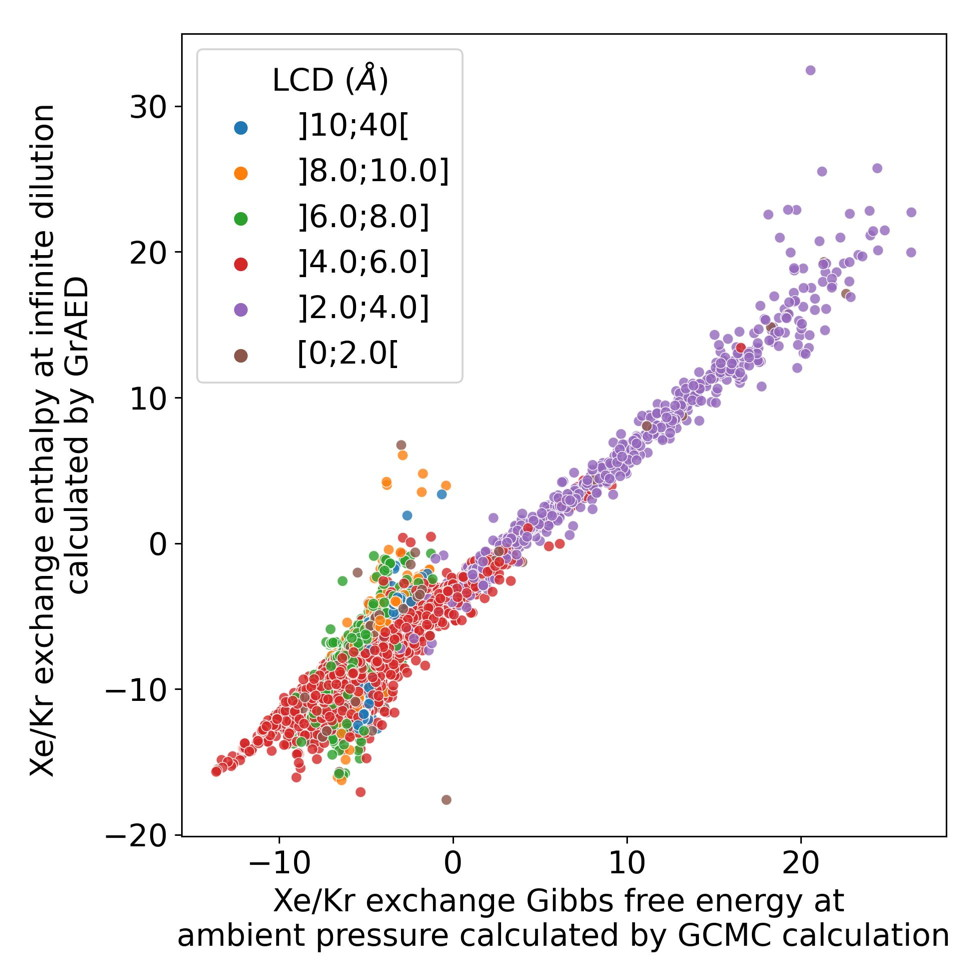
\includegraphics[width=0.45\textwidth]{figures/3-fastsim/G_2080_vs_H_grid_overview.jpg}
    \includegraphics[width=0.45\textwidth]{figures/3-fastsim/G_2080_vs_S_grid_overview.jpg}
    \caption{Comparison of the ambient-pressure Xe/Kr exchange Gibbs free energy calculated by GCMC simulations of RASPA2 with 100,000 cycles and the low-pressure exchange enthalpy (left, in \si{\kilo\joule\per\mole}) and entropy (right, in \si{\kilo\joule\per\mole\per\kelvin}) calculated by the GrAED algorithm (same parameters).}\label{fgr:grid_comp_exc}
\end{figure}

Upon revisiting the exchange thermodynamic quantities that hold greater relevance to the specific context of this thesis, a notable correlation is observed between the exchange enthalpy at low pressure, calculated using GrAED, and the exchange Gibbs free energy at ambient pressure, calculated by GCMC, as illustrated in Figure~\ref{fgr:grid_comp_exc}. However, some discrepancies can be detected around the range of $-10$ and $0$~\si{\kilo\joule\per\mole} for the ambient-pressure exchange free energy. These discrepancies can be attributed to the exchange entropy, which remains relatively stable at around $-0.01$~\si{\kilo\joule\per\mole\per\kelvin}, but exhibits a peak for structures within the aforementioned range of ambient-pressure exchange Gibbs free energy. The strong overall correlation can be explained by the enthalpic nature of the separation process of xenon from krypton (see chapter 2). Furthermore, the problematic range, where the correlation weakens, corresponds to the range associated with a drop in selectivity, as illustrated in Figure~\ref{fgr:G_900K}. These exchange thermodynamic quantities provide valuable insights for distinguishing materials and improving the modeling of the selectivity drop phenomenon. A more quantitative approach will be developed in the subsequent chapter.


\subsubsection{High-temperature quantities}

Although the previous quantities provide valuable insights into modeling the adsorption at ambient pressure, they are still insufficient as they pertain to a state where the atoms are adsorbed only on the most attractive sites. The ambient-pressure state, however, is characterized by adsorption on a more diverse set of sites and the increasing significance of the guest-host interaction, which are the main factors contributing to the selectivity difference between the two pressure conditions identified in the previous chapter.

In this section, a descriptor is introduced that provides a better representation of the energy distribution in the ambient-pressure case by assigning greater weight to the more energetic adsorption sites. The simplest approach was to increase the temperature in the Boltzmann averaging for both the Gibbs free energy and the enthalpy, as defined in equations~\ref{eq:ads_gibbs} and~\ref{eq:ads_enthalpy}. Multiple temperatures were tested, and the temperature yielding the higher correlation coefficient between the adsorption enthalpies (at infinite dilution and ambient pressure) was selected.

A temperature of \SI{900}{\kelvin} was found to be the optimal temperature or describing the ambient-pressure adsorption enthalpy of xenon across the structures of CoRE MOF 2019. This choice resulted in a reduced error (RMSE) of \SI{1.76}{\kilo\joule\per\mole} compared to \SI{2.87}{\kilo\joule\per\mole} for the \SI{298}{\kelvin} case. This improvement has implications for the metrics of exchange free energy and adsorption enthalpy associated with the separation of xenon from krypton. The exchange Gibbs free energy and xenon adsorption enthalpy at ambient pressure exhibit a stronger correlation with their counterparts at lower pressure and higher temperature (\SI{900}{\kelvin}) rather than at \SI{298}{\kelvin}. These observations support the use of higher temperature averaging for describing ambient-pressure selectivity.

This new type of descriptor is particularly promising as it performs better in the high selectivity region, where the standard Boltzmann average at very interesting since it performs better around the high selectivity region, where the standard Boltzmann average at \SI{298}{\kelvin} loses its accuracy (see Figure~\ref{fgr:grid_ambient_selectivity}). As shown in Figures~\ref{fgr:H_900K} and~\ref{fgr:G_900K}, using averaging at higher temperature yields improved performance in describing the behavior of the most selective materials, while compromising the accuracy of descriptions for less selective materials.

In Figure~\ref{fgr:H_900K}, the high-temperature averaging provides a more accurate description of the xenon adsorption enthalpy, with the data points being more centered around the $y=x$ axis, although the correlation is not perfect. Notably, there is greater uncertainty for materials that were initially well predicted as poorly performing materials. The high dispersion around the correlation is likely due to the guest--guest interactions, which are not described in the high temperature averaging but play a non-negligible role in the ambient pressure case.

\begin{figure}[ht]
\centering
  \includegraphics[width=0.45\linewidth]{figures/4-ml/SI_figure/Scatterplot_H1_H0.pdf}
  \includegraphics[width=0.45\linewidth]{figures/4-ml/SI_figure/Scatterplot_H1_H900K.pdf}
  \caption{Scatterplots of the low-pressure xenon adsorption enthalpy at \SI{298}{\kelvin} (left) and at \SI{900}{\kelvin} (right) calculated by the GrAED algorithm against the ambient-pressure xenon adsorption enthalpy at \SI{298}{\kelvin}. Using a higher temperature Boltzmann averaging, the correlation with the ambient-pressure case of interest sigificantly improves. For instance, the R2 coefficient improves from $0.80$ to $0.92$. The RMSE also decreases from \SI{2.87}{\kilo\joule\per\mole} to \SI{1.76}{\kilo\joule\per\mole}. }\label{fgr:H_900K}
\end{figure}

Figure~\ref{fgr:G_900K} shows that the improvement in xenon adsorption enthalpy does not directly translate into improved performance in the exchange Gibbs free energy. The overall correlation is better between the exchange free energy at \SI{298}{\kelvin} and infinite dilution, and the one at ambient pressure (\SI{298}{\kelvin}). However, it can be argued that the exchange free energy at \SI{900}{\kelvin} slightly better describes the materials that experience a selectivity drop, as depicted in Figure~\ref{fgr:grid_ambient_selectivity}. 

\begin{figure}[ht]
\centering
  \includegraphics[width=0.38\linewidth]{figures/3-fastsim/Scatterplot_G1_G0.pdf}
  \includegraphics[width=0.27\linewidth]{figures/3-fastsim/Scatterplot_G1_G900K.pdf}
  \includegraphics[width=0.23\linewidth]{figures/3-fastsim/Scatterplot_G1_G_Xe_900K.pdf}
  \caption{Comparison plot between the low-pressure exchange free energy at \SI{298}{\kelvin} (left) and \SI{900}{\kelvin} (right) calculated by the GrAED algorithm and the ambient-pressure exchange free energy at \SI{298}{\kelvin} calculated by Widom insertion. }\label{fgr:G_900K}
\end{figure}

The utilization of high-temperature averaging enables improved modeling of selectivity in the selective materials that experience a loss of selectivity between low and ambient pressure. These descriptors can quantitatively predict the selectivity at ambient pressure, as demonstrated in the subsequent chapter. Furthermore, these descriptors can provide a qualitative description of the structures that present challenges. It is expected that by leveraging the values obtained through high-temperature averaging, the identification of these problematic structures can be achieved.

\subsubsection{Statistical characterization of the energy distributions}

To quantify the change of selectivity more accurately, it could be interesting to provide statistical information on the distribution of interaction energies for xenon and krypton, calculated using the grid algorithm. By conducting a statistical analysis, the complexity of the pore adsorption process at higher pressure can be explored through the diversity and distribution of energy values (the quantity of the higher energies in comparison to the lower ones, for example). The grid sampling method presented here utilizes all energy values from the sampled points to construct a histogram reprensenting the energy distribution that can be studied to extract meaningful statistical insights.

These statistical measures encompass moments of different orders (up to 4) of the energy distribution, which provide information on the adsorbate--adsorbent interaction energies in the nanopores at higher loading. The shape of the energy distribution enables quantitative assessment of the changes in selectivity. This approach can be considered a means of summarizing the entire energy distribution in a few statistical values, which is a conventional method employed in the field of data science for analyzing distribution data. Two methods are explored in this context: uniform weighting and Boltzmann weighting of the energy distribution. It is worth noting that this subsection does not delve into the average of the Boltzmann-weighted distribution, which typically represents the adsorption enthalpy.

\textbf{Boltzmann weighted distribution}

The Boltzmann weighted distribution consists in assigning a weight $\exp(-\beta E)$ to each sampled point according to the corresponding energy $E$ calculated by the GrAED algorithm. This weighting scheme puts a significantly higher weight on the most negative energy values (corresponding to the most favorable adsorption sites) compared to other points. The unfavorable adsorption sites can be considered negligible due to the exponential scaling, which diminishes the importance of these points in the Boltzmann weighted distribution. This distribution has previously been employed to compute the adsorption enthalpy (the first-order moment or average) and indirectly the Henry constant (sum of the weights used for normalization of the distribution). However, this section will focus on other statistical quantities derived from the distribution, which are not commonly used in describing the thermodynamics of the system.

\begin{figure}[ht]
  \centering
    \includegraphics[width=0.45\textwidth]{figures/3-fastsim/G_2080_vs_enthalpy_std_x_overview.jpg}
    \includegraphics[width=0.45\textwidth]{figures/3-fastsim/G_2080_vs_enthalpy_std_y_overview.jpg}
        \caption{Comparison of the ambient-pressure Xe/Kr exchange Gibbs free energy calculated by GCMC simulations of RASPA2 with 100,000 cycles and the standard deviations of the Boltzmann weighted energy distribution of xenon (left) and krypton (right) calculated by the GrAED algorithm at \SI{298}{\kelvin}.}\label{fgr:enthalpy_std}
\end{figure}

For instance, the standard deviation of the Boltzmann weighted energy distribution is a relevant statistical quantity for evaluating the decline in selectivity. In the previous chapter, the diversity of site attractiveness was identified as a key factors that could explain the drop in selectivity. Therefore, the standard deviation of the energies serves as a useful characterization of the diversity of nature among different adsorption sites. Figure~\ref{fgr:enthalpy_std} presents the calculation of this standard deviation for both xenon and krypton. The values exhibit a higher variation concentrated within a specific range, which aligns with the range of entropy change identified and, more importantly, corresponds to the range where the selectivity drop is observed in Figure~\ref{fgr:G_900K} (between $-10$ and $0$~\si{\kilo\joule\per\mole}). Qualitatively, the standard deviation provides insights into the diversity of pores, which can aid in characterizing the underlying causes of selectivity drop. A higher diversity generally implies a greater probability of experiencing a selectivity drop. However, quantifying the probability of selectivity drop poses a challenge that cannot be adequately addressed by a simple theoretical model alone. Therefore, the next chapter will focus on exploring machine learning models as a means to overcome this limitation.

\begin{figure}[ht]
  \centering
    \includegraphics[width=0.45\textwidth]{figures/3-fastsim/G_2080_vs_enthalpy_skew_overview.jpg}
    \includegraphics[width=0.45\textwidth]{figures/3-fastsim/G_2080_vs_enthalpy_kurt_overview.jpg}
    \caption{Comparison of the ambient-pressure Xe/Kr exchange Gibbs free energy calculated by GCMC simulations of RASPA2 with 100,000 cycles and the skewness (left) and the kurtosis (right) of the Boltzmann weighted energy distribution of xenon calculated by the GrAED algorithm at \SI{298}{\kelvin}.}\label{fgr:enthalpy_skew_kurt}
\end{figure}

Two additional statistical quantities, namely skewness and kurtosis, have been introduced to describe the distribution of energy values. Skewness measures the asymmetry of the distribution, while kurtosis quantifies the ``tailedness'' (the number of values in the tail of the distribution). Skewness is the standardized third moment, and kurtosis is the standardized fourth moment of the distribution. For a random variable $X$ with a mean value of $m$ and a standard deviation $\sigma$, the n-th order moment $\text{M}_{n}(X)$ is defined as:
\begin{equation}
  \text{M}_n(X) = \mathbb{E}\left[{\left(\dfrac{X-m}{\sigma}\right)}^n\right]
\end{equation}
These statistical quantities provide additional insights on the distribution. For instance, if the distribution is skewed towards the most negative pore energies, it indicates a preference for adsorption at higher pressure. Conversely, the opposite skewness would explain a larger drop in selectivity. The overall shape of the distribution requires more than just the standard deviation and mean value to capture the reasons behind the selectivity drop. While having the complete information on the distribution would be ideal, visually comparing structures based on this multidimensional descriptor would be overly complex. The statistical quantities effectively compress the complex energy distribution data.

Figure~\ref{fgr:enthalpy_skew_kurt} further illustrate the range of selectivity values discussed throughout this section. The different statistical quantities introduced in this discussion can be used to sort materials within this range. The skewness and kurtosis values can potentially establish a theoretical link with the previously identified selectivity drop. However, without a model or framework, it is impossible to find the accurate relationship solely by visual observation.

\textbf{Uniformely weighted distribution}

To conclude this overview of the thermodynamic/energetic descriptors derived from the newly developed grid sampling, a more uniformly weighted energy distribution will be examined. The significantly higher energy values corresponding to the overlap with a framework atom are naturally excluded by the sampling process. In this case, a threshold value of $100$~\si{\kilo\joule\per\mole} has been used for the grid sampling, defining a very large overlap range. Energy points below this threshold are considered in the distribution, representing the adsorbable sites (no overlap) that are weighted based on their occupancy of the void volume.

The mean value and standard deviation of this distribution have been analyzed. The mean value shows a weak correlation with the exchange Gibbs energy at ambient pressure. However, the correlation disappears for materials with larger pores, where a more diverse range of energy values is present. The lower mean value in these cases can be attributed to the larger void fraction, resulting in increased weight on the more negative values, but this does not indicate the presence of highly attractive sites, as no Boltzmann weight is applied  --- the exchange free energy does not follow the same trend and returns to more positive values. It is worth mentioning that the values are generally very high due to the use of an energy threshold value of $100$~\si{\kilo\joule\per\mole}, resulting in many points falling within zero to this threshold range, thereby shifting the mean towards these values. Consequently, the statistical analysis of this distribution was not extended beyond the standard deviation. A more refined distribution design should be considered to focus on the negative values, such as lowering the threshold or using a less skewed Boltzmann averaging method (e.g., averaging at higher temperature).

\begin{figure}[ht]
  \centering
    \includegraphics[width=0.45\textwidth]{figures/3-fastsim/G_2080_vs_mean_grid_x_overview.jpg}
    \includegraphics[width=0.45\textwidth]{figures/3-fastsim/G_2080_vs_std_grid_x_overview.jpg}
    \caption{Comparison of the ambient-pressure Xe/Kr exchange Gibbs free energy calculated by GCMC simulations of RASPA2 with 100,000 cycles and the mean values (left) and the standard deviation (right) of the uniformly weighted energy distribution of xenon calculated by the GrAED algorithm at \SI{298}{\kelvin}.}\label{fgr:energy_dist_mean_std}
\end{figure}

The standard deviation of this distribution has a lower value for materials with larger pores, as depicted in Figure~\ref{fgr:energy_dist_mean_std}. This observation can be attributed to a higher concentration of points near the average value of the energy (around $0$ and $10$~\si{\kilo\joule\per\mole}), as depicted by the left plot in the figure. For materials with a standard deviation between $20$ and $40$~\si{\kilo\joule\per\mole}, it seems clear that their exchange free energy does not exceed $-8$~\si{\kilo\joule\per\mole}, indicating that they are not among the top selective materials. Therefore, the presented standard deviation aids in identifying materials that could be promising at low pressure but do not exhibit promising behavior in practice.

To improve this approach, the utilization of a higher temperature Boltzmann average for the distribution weights was explored, without necessarily employing a temperature of \SI{900}{\kelvin}. Additionally, a uniformly weighted average was tested on an energy distribution using different energy thresholds (zero or the mean kinetic energy of a gas $1.5k\e{B}T$). The underlying concept behind these explorations is to characterize a higher energy state close to the state at ambient pressure. Furthermore, higher-order moments can be tested to provide a more picture of the distribution. 

\vspace{2cm}

This GrAED algorithm proves to be particularly efficient in sampling energies for structures characterized by high symmetry and a large occupied volume. The highly accurate description provided by the grid enables the calculation of additional descriptive metrics, which can be valuable not only for describing adsorption at infinite dilution but also for investigating correlations with selectivity values at higher pressures. Finally, detailed computations on the GrAED sampling technique can be accessed online at \url{github.com/coudertlab/GrAED}.


\section{From description to prediction}

In this chapter, a comprehensive overview of fast sampling techniques for evaluating adsorption performance at infinite dilution was provided, excluding the standard Widom insertion method discussed in the previous chapter. The effectiveness of these quantities in describing the thermodynamics of adsorption in nanoporous materials was demonstrated by comparing them to conventional methods. The next step is to examine their predictive value in determining Xe/Kr selectivity under physical conditions closer to industrial settings.

For instance, in the previous section, each thermodynamic descriptor derived from grid sampling was individually examined and compared to ambient-pressure conditions. However, this approach has limitations, as it only offers a descriptive understanding and cannot provide predictions. Moreover, the limited dimensions in visualization restrict the breadth of correlations. While certain key features of the most selective materials (pores adapted to the kinetic diameter, pore shape that maximizes the interactions, etc.) were identified, the correlation-based approach also revealed inherent weaknesses. Understanding high-pressure selectivity using quantities solely based on a host--guest interaction energy grid proves challenging. To overcome these challenges, modern approaches employ statistical learning to capture this relationship using a sufficiently large set of structures with some computed properties. In the upcoming chapter, the potential of these novel descriptors for predicting selectivity values beyond the infinitely diluted case will be explored, all while significantly reducing computational costs.


\OnlyInSubfile{\printglobalbibliography}

\end{document}